
\documentclass[
  fontsize=10pt, % Base font size
  twoside=true, % Use different layouts for even and odd pages (in particular, if twoside=true, the margin column will be always on the outside)
  % open=any, % If twoside=true, uncomment this to force new chapters to start on any page, not only on right (odd) pages
  secnumdepth=1, % How deep to number headings. Defaults to 1 (sections)
  %chapterprefix=true, % Uncomment to use the word "Chapter" before chapter numbers everywhere they appear
  %chapterentrydots=true, % Uncomment to output dots from the chapter name to the page number in the table of contents
  numbers=noenddot, % Comment to output dots after chapter numbers; the most common values for this option are: enddot, noenddot and auto (see the KOMAScript documentation for an in-depth explanation)
  % draft=true, % If uncommented, rulers will be added in the header and footer
  % overfullrule=true, % If uncommented, overly long lines will be marked by a black box; useful for correcting spacing problems
]{kaobook}

% Choose the language
\usepackage[english]{babel} % Load characters and hyphenation
\usepackage[english=british]{csquotes}  % English quotes

% Load packages for testing
\usepackage{blindtext}
%\usepackage{showframe} % Uncomment to show boxes around the text area, margin, header and footer
%\usepackage{showlabels} % Uncomment to output the content of \label commands to the document where they are used

% Load the bibliography package
% \usepackage{styles/kaobiblio}
% \addbibresource{book-template.bib} % Bibliography file

% Load the package for hyperreferences
\usepackage{kaorefs}

% Load mathematical packages for theorems and related environments. NOTE: choose only one between 'mdftheorems' and 'plaintheorems'.
% \usepackage{styles/mdftheorems}
%\usepackage{styles/plaintheorems}
\usepackage[framed=true]{kaotheorems}

\usepackage{float}
\newfloat{floatbox}{tb}{ext2}

\usepackage{pdfpages}

% \graphicspath{{images/}{./}} % Paths in which to look for images

\makeindex[columns=3, title=Index, intoc] % Make LaTeX produce the files required to compile the index

\makeglossaries % Make LaTeX produce the files required to compile the glossary

\makenomenclature % Make LaTeX produce the files required to compile the nomenclature

%-- new box environments
\definecolor{redish}{HTML}{F7E0E0}
\definecolor{blueish}{HTML}{DDECF1}
\definecolor{greenish}{HTML}{E6E6E6}
\newmdenv[
  style=kaoboxstyle,
  backgroundcolor=redish,
  frametitlebackgroundcolor=redish,
]{kaobox-practice}
\newmdenv[
  style=kaoboxstyle,
  backgroundcolor=blueish,
  frametitlebackgroundcolor=blueish,
]{kaobox-toread}
\newmdenv[
  style=kaoboxstyle,
  backgroundcolor=greenish,
  frametitlebackgroundcolor=greenish,
]{kaobox-info}
\newcommand{\youtube}[2][0pt]{%
  \marginnote[#1]{
    \begin{kaobox}[
      backgroundcolor=blueish,
      frametitlebackgroundcolor=blueish
    ]
    \center{\faYoutube\ \href{https://#2}{#2}}
    \end{kaobox}
  }
  \vspace{1cm}
}

%----------------------------------------
% HL
%----------------------------------------

% \usepackage[backend=biber,natbib=true,maxcitenames=2,maxbibnames=10,giveninits=true,isbn=false,doi=false,url=false,defernumbers=true,style=numeric,sorting=ydnt]{biblatex} 
\usepackage[backend=bibtex,natbib=true,style=authoryear,citestyle=authoryear,maxcitenames=2,maxbibnames=10,giveninits=true,isbn=false,doi=false,dashed=false]{biblatex}
\bibliography{refs/tb} % Bibliography file
%-- remove the In:
\renewbibmacro{in:}{}
%-- remove the "" before/after the title of the paper
\DeclareFieldFormat[article, inbook, incollection, inproceedings, misc, thesis, unpublished]{title}{#1}



% Command to print a citation in the margins
\newcommand{\sidecitet}[1]{% The optional parameter is the 
%vertical shift; 
%the mandatory one is the citation key
  \citet{#1}% With this we print the marker in the text and add the item to the 
  %bibliography at the end \margincitation
  \marginnote{\citeauthor*{#1} (\citeyear{#1}), \citetitle{#1}\\}% 
  %Create a marginnote for each item
}

\newcommand{\sidecitep}[1]{% The optional parameter is the 
%vertical shift; 
%the mandatory one is the citation key
  \citep{#1}% With this we print the marker in the text and add the item to the 
  %bibliography at the end \margincitation
  \marginnote{\citeauthor*{#1} (\citeyear{#1}), \citetitle{#1}\\}% 
  %Create a marginnote for each item
}

\renewcommand{\ie}{ie}
\renewcommand{\eg}{eg}



\setcounter{margintocdepth}{1}
\setcounter{tocdepth}{1}
\setcounter{secnumdepth}{3}

\usepackage{subcaption}
\usepackage{fontawesome}
\usepackage{gensymb}
\usepackage{xurl}
\usepackage{hyperref}
\hypersetup{breaklinks=true}
\usepackage{siunitx}



%----------------------------------------------------------------------------------------

\begin{document}

%----------------------------------------------------------------------------------------
% BOOK INFORMATION
%----------------------------------------------------------------------------------------


\title{Computational modelling of terrains}
\author{Hugo Ledoux \hspace{10mm} Ken Arroyo Ohori\\ Ravi Peters \hspace{17mm} Maarten Pronk}
\date{\texttt{v2024.0}}

% \publishers{\includegraphics[width=\linewidth]{front-back/imhof.png}}

%----------------------------------------------------------------------------------------

\frontmatter % Denotes the start of the pre-document content, uses roman numerals

%----------------------------------------------------------------------------------------
% OPENING PAGE
%----------------------------------------------------------------------------------------

%\makeatletter
%\extratitle{
% % In the title page, the title is vspaced by 9.5\baselineskip
% \vspace*{9\baselineskip}
% \vspace*{\parskip}
% \begin{center}
%   % In the title page, \huge is set after the komafont for title
%   \usekomafont{title}\huge\@title
% \end{center}
%}
%\makeatother

%----------------------------------------------------------------------------------------
% COPYRIGHT PAGE
%----------------------------------------------------------------------------------------

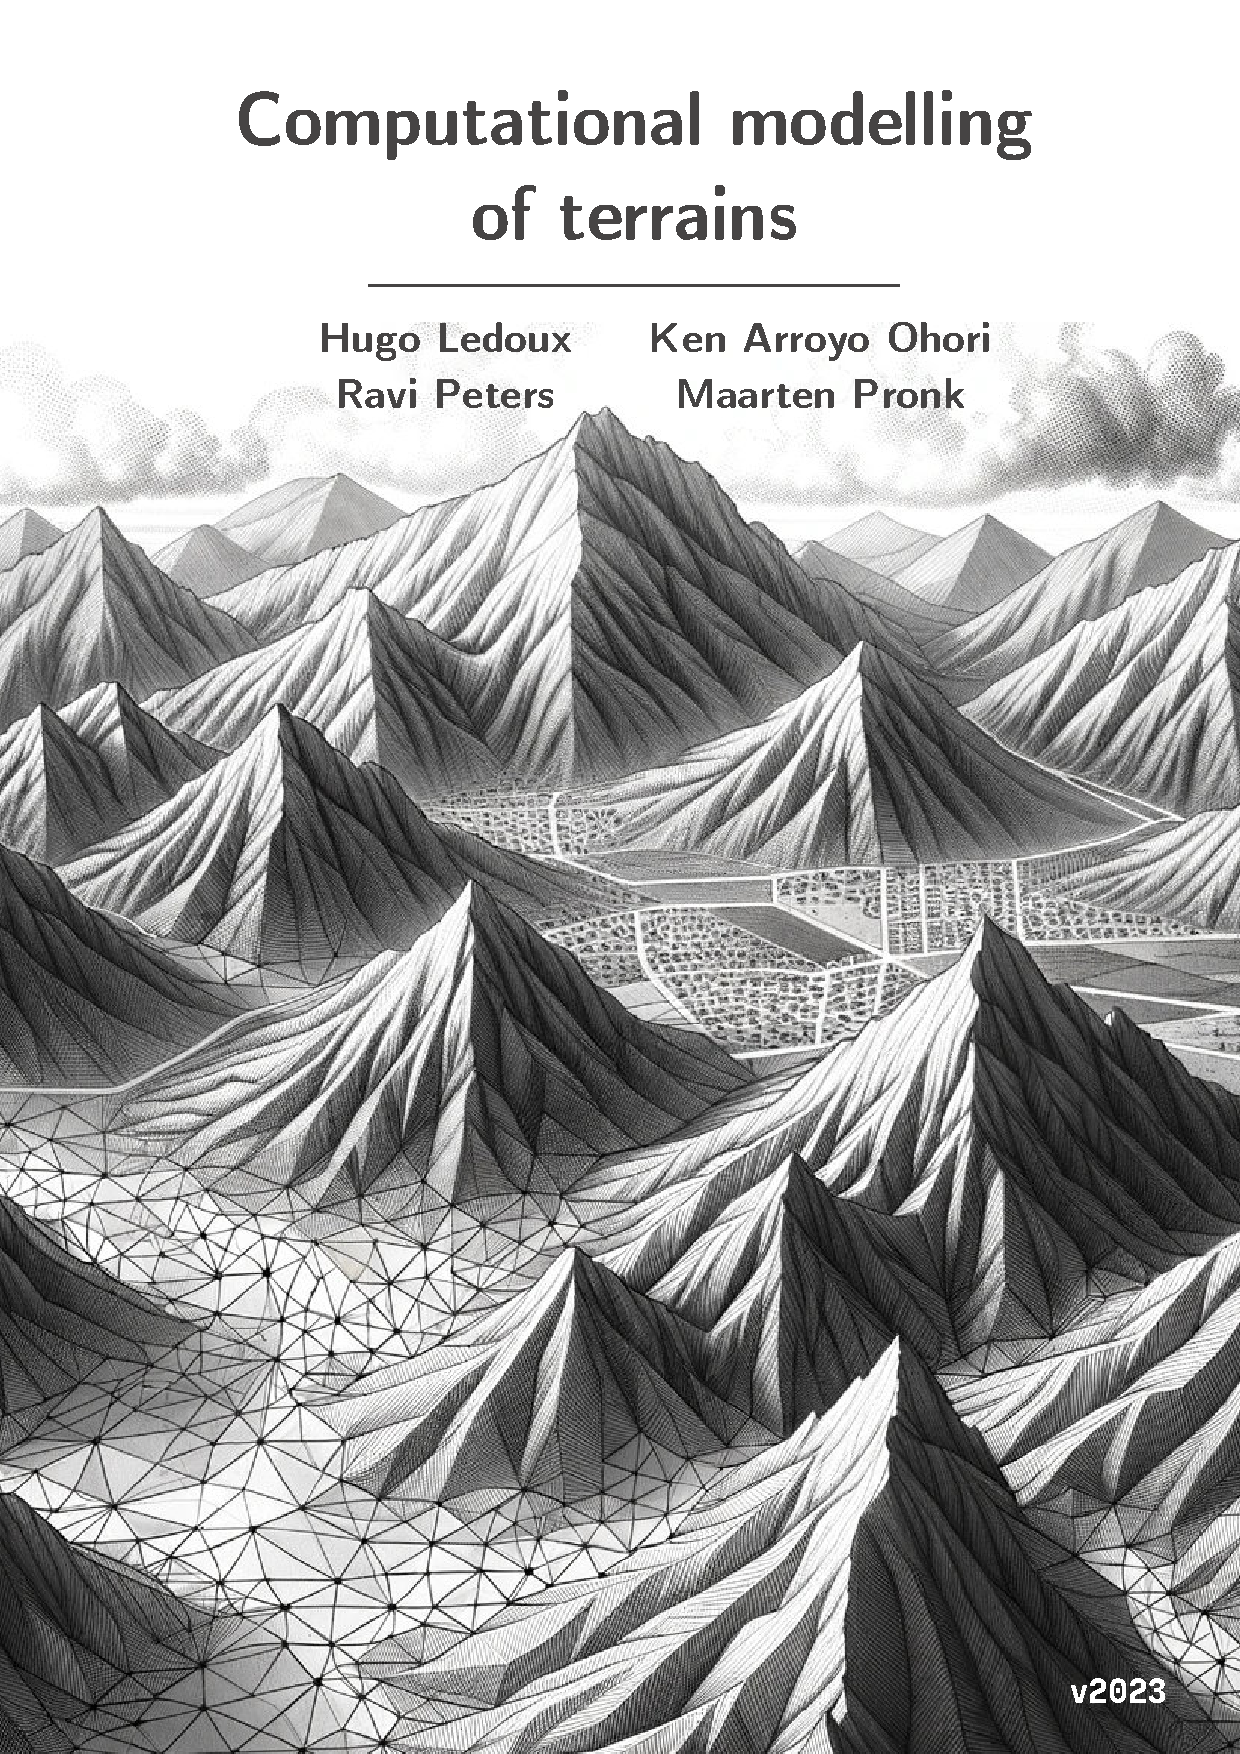
\includepdf{cover/cover_front.pdf}
\cleardoublepage


%!TEX root = ../terrainbook.tex


\makeatletter
% \uppertitleback{\@titlehead} % Header

\lowertitleback{
  
\textcopyright\ 2023 \, Hugo Ledoux, Ken Arroyo Ohori, Ravi Peters, and Maarten Pronk

\medskip

\ccLogo\ \ccAttribution\ This work is available under a Creative Commons Attribution 4.0 International License.
For license details, see \url{http://creativecommons.org/licenses/by/4.0/}

\medskip

\texttt{v0.9 [2022--11--14]}
\\
\texttt{v0.8 [2021--11--08]}
\\
\texttt{v0.7 [2020--11--09]}
\\
\texttt{v0.6 [2019--11--11]}

\medskip
\medskip

\textbf{Download latest version} \\
The latest version of this book can be downloaded in PDF at\\ 
\url{https://github.com/tudelft3d/terrainbook/releases}

\medskip

\textbf{Extra material} \\
Most chapters have a short YouTube video explaining the key concepts, and some chapters have extra material. Available at\\
\url{https://tudelft3d.github.io/terrainbook/videos}

\medskip

\textbf{Source code} \\
The source code of the book, in \LaTeX, is available at\\
\url{https://github.com/tudelft3d/terrainbook}

\medskip

\textbf{Errors? Feedback?} \\
Please report errors or potential improvements at\\
\url{https://github.com/tudelft3d/terrainbook/issues}

\medskip

\textbf{Colophon} \\
This book was typeset with \LaTeX\ using the \texttt{kaobook} class.
% \mbox{{\fanciestfont{}Feijoa}}, \texttt{GT Pressura} and $\mathrm{Asana\ Math}$ typefaces.
The figures were created using Ipe, OmniGraffle, Affinity Designer, or Blender.
The cover image is generated by DALL·E 3.
 

}
\makeatother







%----------------------------------------------------------------------------------------
% OUTPUT TITLE PAGE AND PREVIOUS
%----------------------------------------------------------------------------------------

\maketitle

%----------------------------------------------------------------------------------------
% PREFACE
%----------------------------------------------------------------------------------------

%!TEX root = ../terrainbook.tex

% About this book
% from a course, bundle of lecture notes
% link to videos
% acknowledgements


\chapter*{Preface}

This book presents an overview of algorithms and methodologies to reconstruct, manipulate, and extract information from terrains.

It covers different representations of terrains (\eg\ TINs, rasters, point clouds, contour lines) and presents techniques to handle large datasets.

% DTM are often only grid and TINS
% Modelling of terrains is one aspect of GIS that significantly changed with the arrival of new acquisition technologies such as airborne laser scanners and radar (SRTM), and yet books are often written years ago.


\paragraph*{Open material.}
This book is the bundle of the lecture notes that we wrote for the course \emph{Digitial terrain modelling} (GEO1015) in the MSc Geomatics at the Delft University of Technology in the Netherlands.
The course is tailored for MSc students who have already followed an introductory course in GIS and in programming.

Each chapter is a lesson in the course, and each lesson is accompanied by a video introducing the key ideas and/or explaining some parts of the lessons.
All the videos are freely available online on the website of the course: \url{https://3d.bk.tudelft.nl/courses/geo1015/}


\paragraph*{Who is this book for?}
The book is written for students in Geomatics at the MSc level, but we believe it can be also used at the BSc level.

Prerequisites are: GIS, background in linear algebra, programming course at the introductory level.


\paragraph*{Acknowledgements.}
We thank Balázs Dukai for help in proof-reading, and all the students of the first year of the course (2018--2019) who helped by pointing out errors and typos.
Also, the following students of the course all made pull requests to fix errors/typos: Chen Zhaiyu, Ardavan Vameghi, Li Xiaoai, Ivan Pađen, Anna Lisa Labaar.








%----------------------------------------------------------------------------------------
% TABLE OF CONTENTS & LIST OF FIGURES/TABLES
%----------------------------------------------------------------------------------------

\begingroup % Local scope for the following commands

% Define the style for the TOC, LOF, and LOT
%\setstretch{1} % Uncomment to modify line spacing in the ToC
%\hypersetup{linkcolor=blue} % Uncomment to set the colour of links in the ToC
\setlength{\textheight}{23cm} % Manually adjust the height of the ToC pages

% Turn on compatibility mode for the etoc package
\etocstandarddisplaystyle % "toc display" as if etoc was not loaded
\etocstandardlines % "toc lines as if etoc was not loaded

\tableofcontents % Output the table of contents

% \listoffigures % Output the list of figures

% Comment both of the following lines to have the LOF and the LOT on different pages
% \let\cleardoublepage\bigskip
% \let\clearpage\bigskip

% \listoftables % Output the list of tables

\endgroup

%----------------------------------------------------------------------------------------
% MAIN BODY
%----------------------------------------------------------------------------------------

\mainmatter 
\setchapterstyle{kao} % Choose the default chapter heading style

%!TEX root = ../terrainbook.tex

\setchapterpreamble[u]{\margintoc}
\chapter{What is a terrain?}%
\label{chap:whatisterrain}
\labch{whatisterrain}

\graphicspath{{whatisterrain/}}

%%%%%%%%%%%%%%%%%%%%%%%%%%%%%%%%%%%%%%%%%%%%%%%%%%%
% DTM == representation of the Earth's surface
% Dimensionality of DTM (2D, 2.5D, 2.75D, 3D)
% DTM, DSM, DEM
% nDSM: https://www.stadtentwicklung.berlin.de/umwelt/umweltatlas/ed610_03.htm
% Representation of DTMs in computers
%   - a DTM is a 2D field (object vs field discussion from GEO1002)
%   - 6 common representations: regularly spaced sample points; irregularly spaced sample points; contour lines; rectangular cells (raster); triangulated irregular networks (TIN); planar partition with arbitrary polygons.
%   - some are incomplete
%   - discussion data model vs data structure?




% \begin{center}
%   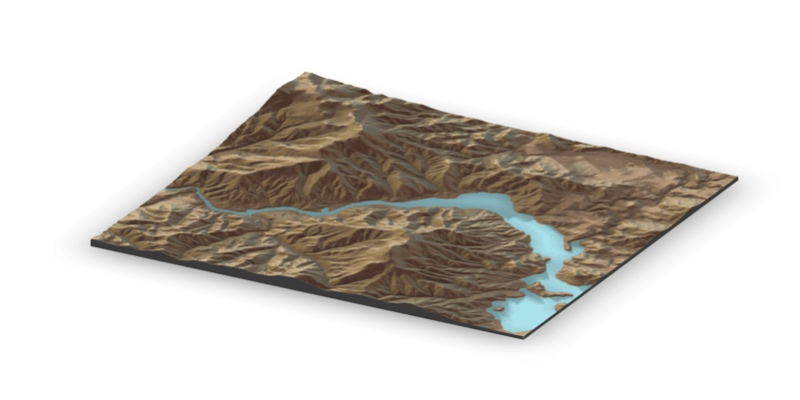
\includegraphics[width=0.95\linewidth]{figs/header.jpg}
% \end{center}


Defining what a terrain, also called a \emph{digital terrain model} (DTM), is not simple because there is no universal agreement, neither among practitioners nor in the scientific literature.
Different terms are used, often interchangeably.

In most cases, we can state that:

\begin{quote}
A terrain is a representation of the Earth's surface. 
It gives us the \emph{elevation}, which is the height above/below a certain reference point (a vertical datum)
\end{quote}

However, the ``Earth's surface'' is also not a clear concept, since several objects on it can be present, \eg\ man-made structures like buildings, roads, power lines, and bridges, and other objects like trees.

\begin{marginfigure}
  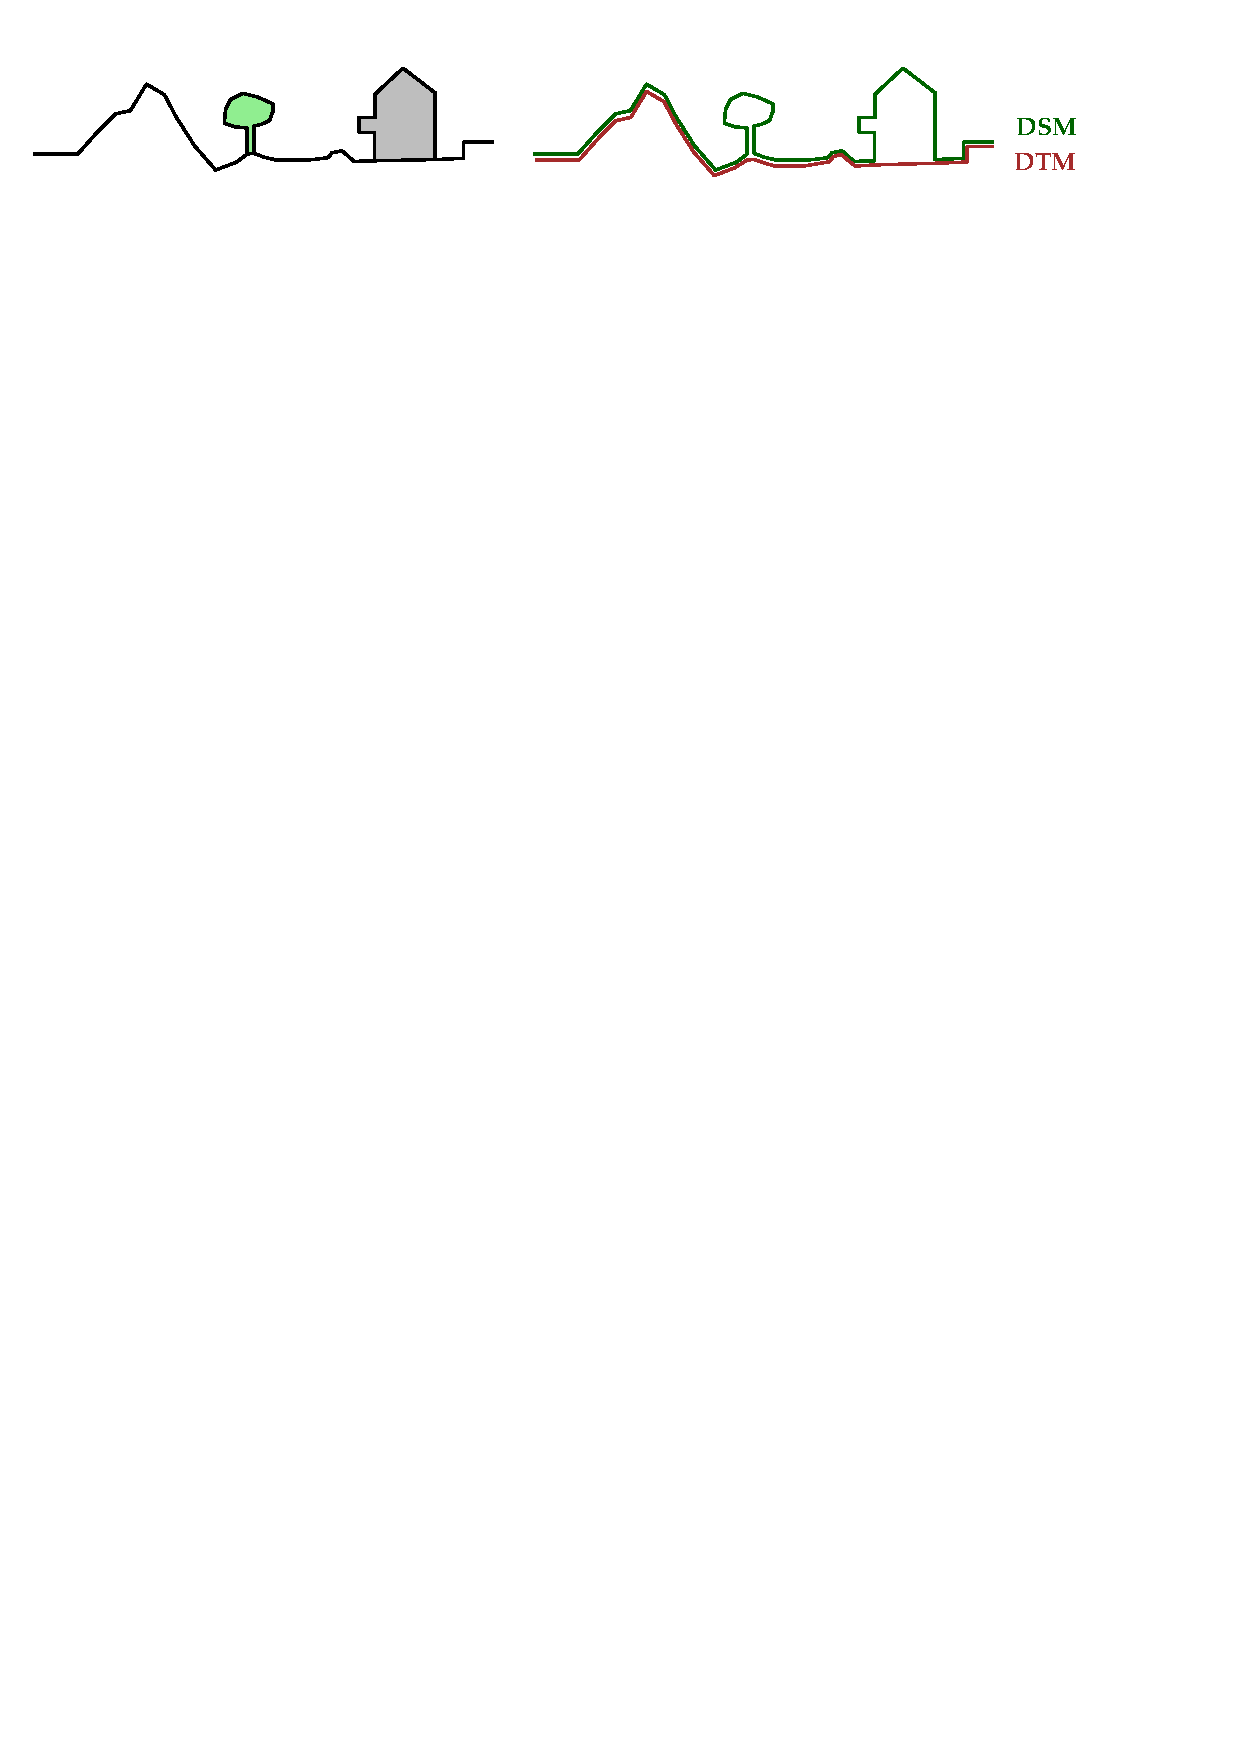
\includegraphics{figs/dtmdsm}
  \caption{\textbf{Top}: a terrain with a mountain, a tree, and a building. \textbf{Bottom}: its DSM and DTM.}%
\labfig{fig:dtmdsm}
\end{marginfigure}
We use the following definitions in this course (see \reffig{fig:dtmdsm}):
\begin{description}
  \item[DEM] (\textbf{D}igital \textbf{E}levation \textbf{M}odel). In the literal meaning of the term, it is simply a model of the elevation. A DEM is either a DSM or a DTM\@. 
  \item[DTM] (\textbf{D}igital \textbf{T}errain \textbf{M}odel). The surface of the Earth is the \emph{bare-earth}, that is no man-made objects or vegetation is present. 
  \item[DSM] (\textbf{D}igital \textbf{S}urface \textbf{M}odel). The surface includes all objects and structures on the terrain.
\end{description}

It should be noticed that in some countries a DEM is often synonymous with a grid of elevation (see below).


%%%
%
\section{Dimensionality of DTMs}

The term ``3D'' is misleading in a DTM context, as it is in a GIS context, because it might refer to three different concepts: 2.5D, 2.75D, and 3D (see \reffig{fig:dimgis}).
\begin{figure}[b]
  \centering
  \begin{subfigure}[b]{0.45\linewidth}
    \centering
    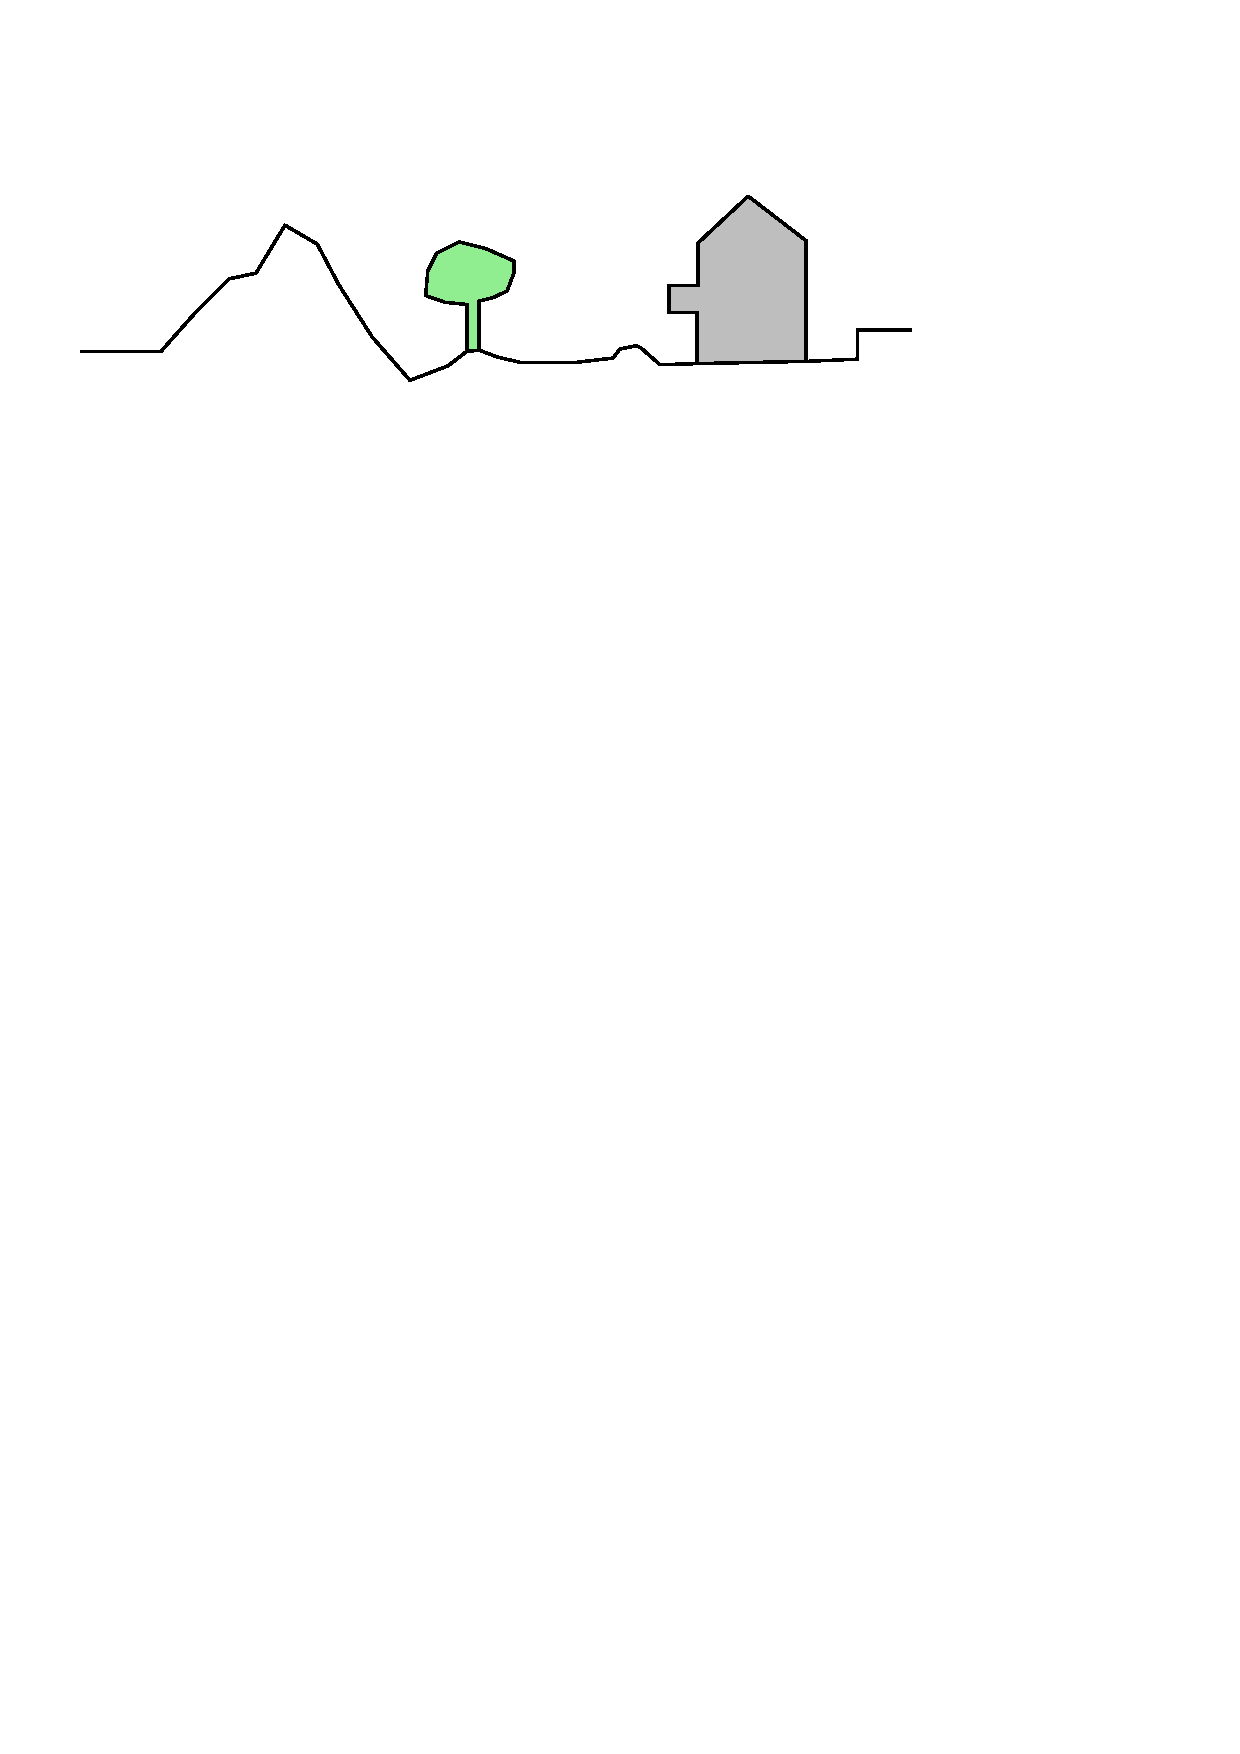
\includegraphics[page=1,width=\linewidth]{figs/dimgis}
    \caption{A terrain}\labfig{fig:dimgis:1}
  \end{subfigure}%
  \qquad %-- that adds some space between th 2 figures
  \begin{subfigure}[b]{0.45\linewidth}
    \centering
    \includegraphics[page=6,width=\linewidth]{figs/dimgis}
    \caption{2.5D modelling}\labfig{fig:dimgis:25}
  \end{subfigure}%
  \qquad %-- that adds some space between th 2 figures
  \begin{subfigure}[b]{0.45\linewidth}
    \centering
    \includegraphics[page=5,width=\linewidth]{figs/dimgis}
    \caption{2.75D modelling}\labfig{fig:dimgis:275}
  \end{subfigure}%
  \qquad %-- that adds some space between th 2 figures
  \begin{subfigure}[b]{0.45\linewidth}
    \centering
    \includegraphics[page=4,width=\linewidth]{figs/dimgis}
    \caption{Volumetric modelling, or full 3D}\labfig{fig:dimgis:3}
  \end{subfigure}%
  \caption{Different meanings for `3D GIS' in the context of terrains.}
\labfig{fig:dimgis}
\end{figure}


\subsection{2.5D} 
\labsec{ddd}
What is usually used for modelling terrains: a surface (which is a topologically a 2D object; also called a 2-manifold) is embedded in 3D space, and each location ($x,y$) is assigned to one and only one height $z$.
% \marginnote{Text of the note}
In other words, the surface can be projected to the $xy$-plane and maintain its topology.
When we refer to terrains in this course, this is what is usually mean, unlike explicitly stated otherwise.
This is often what is used in GIS software, and both the well-known raster/grid  is such a case.
Observe that this restricts the real-world cases that can be modelled because, as shown in \reffig{fig:dimgis}b, vertical surfaces (\eg\ walls of a building if we model all man-made objects with the terrain to construct a digital surface model), overfolds (\eg\ the balcony of a house) and caves are impossible to represent.
As shown in the figure, these are modelled as nearly vertical surfaces; in practice the wall of building could deviate by for instance 1 degree from the vertical. 

\subsection{2.75D} 
This also refers to a surface (a 2-manifold) but unlike for the 2.5D case, the surface is not restricted to be projectable to the 2D plane (see \reffig{fig:dimgis}c).
Thus, more than one $z$ value is allowed for a given location ($x,y$).
The term '2.75D' was coined because: it is more than 2.5D, but less than 3D.
The surface represents the exterior of all objects/features together, and vertical walls are allowed.
Surface modelling is popular in CAD, but in the GIS it is rather rare.
We are not aware of any popular GIS software that allows us to model a terrain as a 2.75D and perform operations on it.

\subsection{Full 3D, or volumetric modelling} 
This refers to the modelling of not only the boundaries of objects, but also of the interior of these.
Notice for instance in \reffig{fig:dimgis}d that each building is represented with a solid.
The volume of buildings can therefore be calculated (since the ground floor of buildings would be modelled for instance), while with the other variations it is not possible. 
Such a representation is usually done with a 2.5D terrain (although a 2.75D could also be used) and a set of buildings/objects that are connected to the terrain.



%%%
%
\section{2.5D terrain == field}
\index{field}

In the context of this course, we assume that a terrain is a 2.5D object, and therefore a terrain can be considered as a \emph{field}.
A field is a model of the spatial variation of an attribute $a$ over a spatial domain, which in our case is $\mathbb{R}^2$, the two-dimensional Euclidean space.
It is modelled by a function mapping one point $p$ in $\mathbb{R}^2$ to the value of $a$, thus 
\[
  a = f(p)
\]
The function can theoretically have any number of independent variables, but in the context of a terrain the function is usually bivariate ($x,y$).

%

The representation of a field in a computer faces many problems. 
First, fields are continuous functions, and, by contrast, computers are discrete machines. 
Fields must therefore be \emph{discretised}, \ie\ broken into finite parts.
\index{discretisation}
Second, in practice it is usually impossible to measure continuous phenomena everywhere, and we have to resort to collecting samples at some finite locations and reconstructing fields from these samples.
The discretisation task therefore begins at the acquisition phase, and is affected by the acquisition tools and techniques (more about this in \refchap{chap:acquisition}).
This fact is aggravated for fields as found in GIS-related disciplines because, unlike disciplines like medicine or engineering, we seldom have direct and easy access to the whole object of interest.


%%%
\subsection{What is needed to represent a field/terrain?}

To represent a terrain in a computer, and be able to manipulate it (\ie\ edit the terrain and extract information such as slope), two things are needed:
\begin{enumerate}
  \item a set of samples that were collected to study the terrain, for instance a point cloud obtained from airbone laserscanning or photogrammetry (see \refchap{chap:acquisition} for details).
  \item a set of rules to obtain one and only one elevation value at any location ($x,y$); in other words, to reconstruct the continuity of the surface from the discrete samples.
  This operation is referred to as spatial interpolation (Chapters~\ref{chap:interpol} and~\ref{chap:kriging}). 
\end{enumerate}


%%%
\subsection{Strategy \#1: points + global interpolation function.}
This means storing the original sample points with the parameters of the \emph{global} spatial interpolation method that is best suited to the distribution of the samples and their accuracy.
Global methods are for instance inverse-distance to a power, natural neighbours, or Kriging.
This strategy is used because one can compactly represent a field (only the samples and a few parameters need to be stored).

Notice that this strategy permits us to reconstruct the continuity of a terrain from the samples by calculating the value of the elevation, but that this value is \emph{not} persistently stored in memory.
It is therefore less used in practice than the next strategy, which allows us to permanently store the terrain in a file and avoids us recomputing every time al the needed elevation values.


%%%
\subsection{Strategy \#2: piecewise spatial models}
This means that the spatial interpolation function used is \emph{piecewise} (instead of being global).
\marginnote{piecewise function}
\index{piecewise function}
That is, the two-dimensional domain of the terrain (the $xy$-plane) is tessellated, or partitioned, into several pieces, and for each of these we assign an interpolation function describing the spatial variation in its interior.
This function is usually a simple mathematical function:
\begin{itemize}
  \item constant function: the value of the modelled attribute is constant within one cell;
  \item linear function;
  \item higher-order function.
\end{itemize}

%

In general, we  classify the tessellations of space into three categories (as shown in \reffig{fig:tesstypes}): \emph{regular}, \emph{irregular}, and \emph{hierarchical}.
\begin{marginfigure}
  \centering
  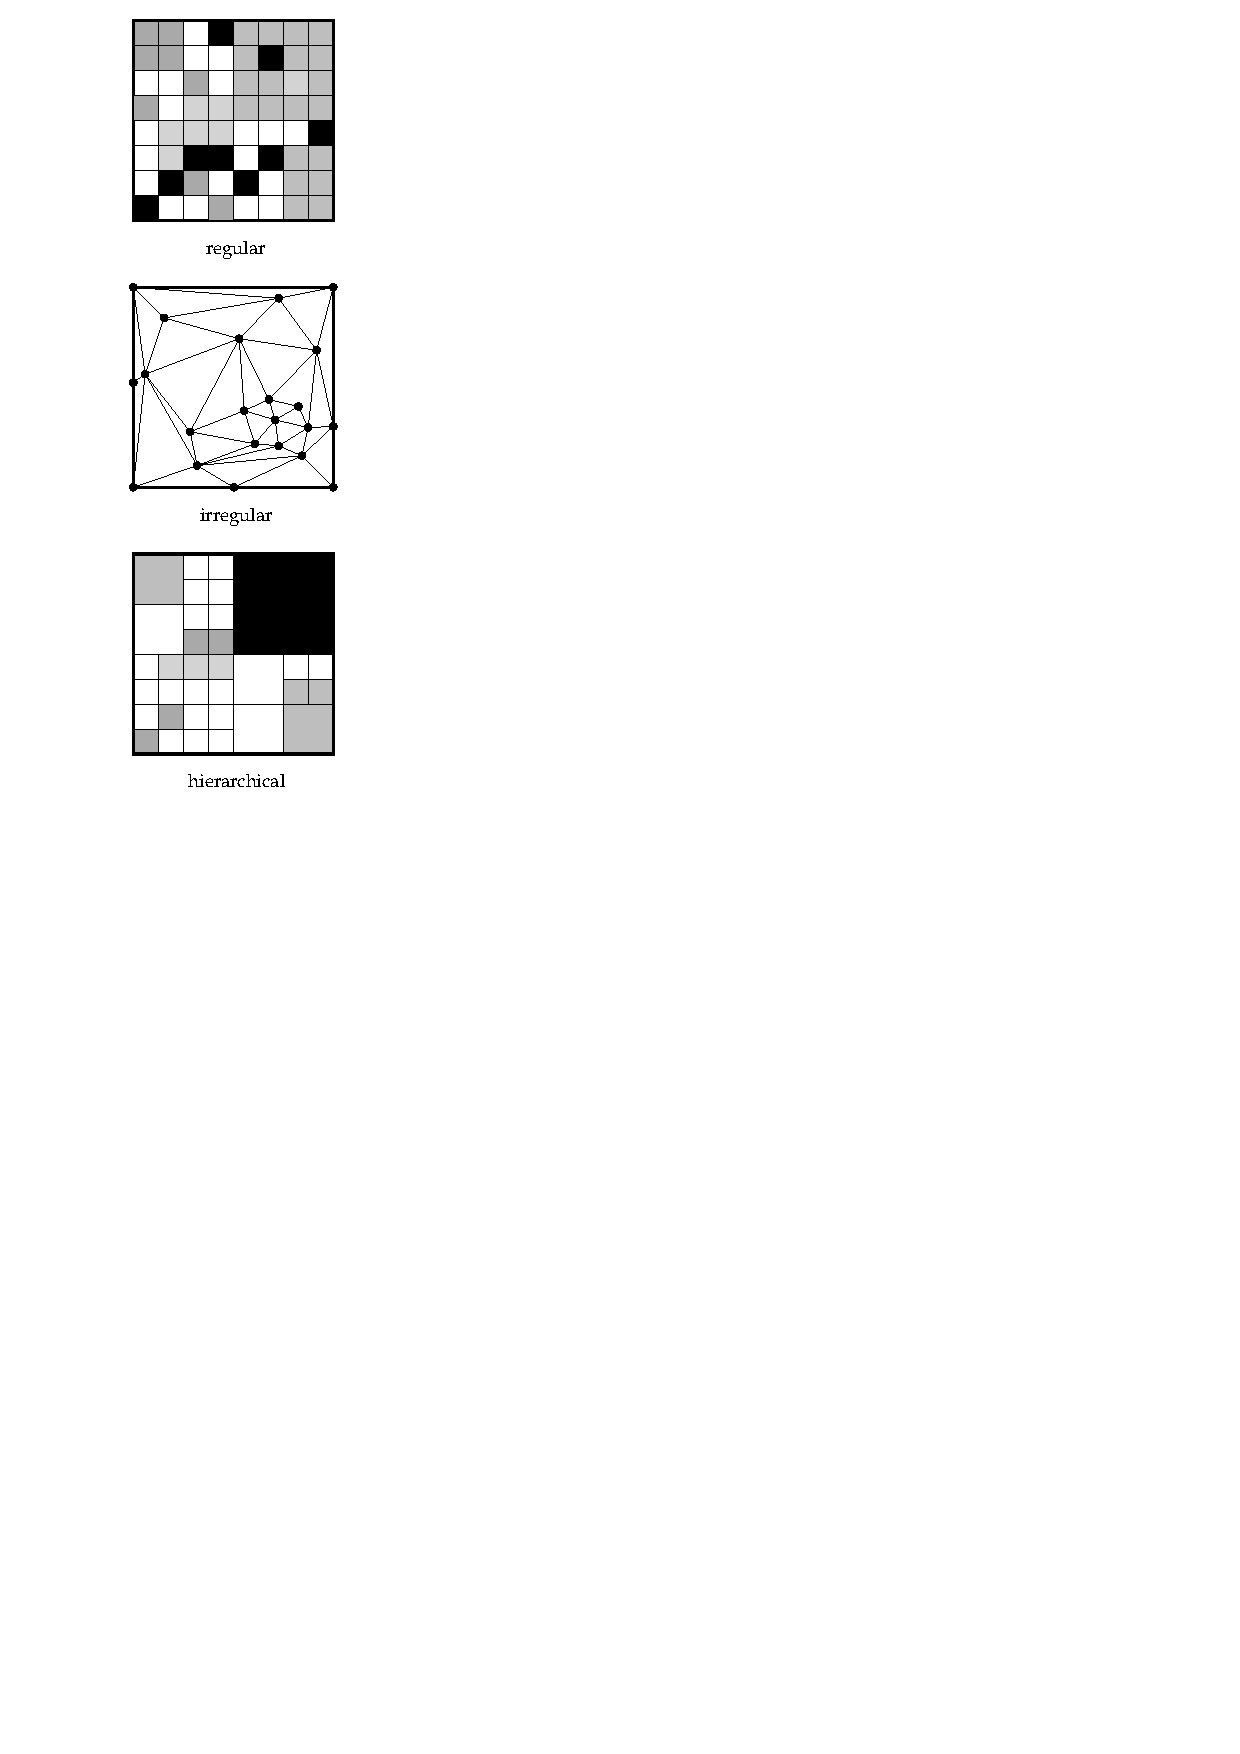
\includegraphics[width=0.7\textwidth]{figs/tesstype}
  \caption{Type of tessellations.}% 
\labfig{fig:tesstypes}
\end{marginfigure}

%

Piecewise models typically imply that a supporting data structure is constructed, and stored, to represent the tessellation.
% (it is however possible to construct on-the-fly some well-known structures only when they are needed since they have formal rules).
Some of these tessellations partition arbitrarily the space, while some are based on the spatial distribution of the sample points.


%%%
%
\section[Data models for terrains]{Data models for representing terrains in a computer}

\subsection{Spatial data models $\neq$ data structures}

In the GIS literature, there exists a confusion between the terms ``spatial model'' and ``data structure''. 
The confusion originates from the fact that object and field views of space are usually implemented in a GIS with respectively vector and raster models. 
However, this is not always the case as TINs can be used for fields for instance.
A ``spatial data model'' offers an \emph{abstract} view of a data structure, it is an abstraction of the reality.
A data structure is the specific implementation of a spatial data model, and deals with storage, which topological relationships are explicitly stored, performance, etc.
The same spatial data model can therefore be implemented with different data structures.



%%%
\subsection{Regular Tessellations} 

As shown in \reffig{fig:tesstypes}a, all the cells have the same shape and size.
The most common regular tessellation in GIS and in terrain modelling is by far the grid (or raster representation), in which the cells are squares in 2D (usually called \emph{pixels}, a portmanteau of `picture' and `element', as an analogy to digital images).
However, while they are not common in practice, other regular shapes are possible, such as hexagons or triangles.

%

Observe that a regular tessellation often arbitrarily tessellates the space covered by the field without taking into consideration the objects embedded in it (the samples). 
This is in contrast with irregular tessellations in which, most of the time, the shape of the cells constructed depends on the samples.

In practice this means that, if we have a terrain stored as a regular tessellation we can assume that it was constructed from a set of samples by using spatial interpolation.
Converting sample points to cells is not optimal because the original samples, which could be meaningful points such as the summits, valleys or ridges of a terrain, are not necessarily present in the resulting tessellation. 
There is a loss of information, since the exact location of the meaningful points are lost.
% Also, when a practitioner has access to a grid, she often does not know how it was constructed and what interpolation method was used, unless meta-data are available.

%

\paragraph{Concrete example: a 2D grid.}
A 2D grid, stored for instance with the GeoTIFF format, is thus a piecewise representation of a 2D field: a regular tessellation where each cell has a constant function.
The value assigned to each cell is an estimation previously obtained by spatial interpolation.
However, for a given grid, it is usually unclear if the value of a cell is for its centre, or for one of its vertices (and if it is the case, for which one?).
Different formats have different rules, and converting a field represented with one format to another one (while retaining the same cell resolution and spatial extent) can shift the value from the centre to the top-left corner for instance.

%

The wide popularity of regular tessellations in terrain modelling is probably due to simplicity and to the fact that they permit us to easily integrate 2D remote sensing images and terrains.
Indeed, a grid is naturally stored in a computer as an array (each cell is addressed by its position in the array, and only the value of the cell is stored), and thus the spatial relationships between cells are implicit. 
This is true for any dimensions, thus, contrary to other tessellations, grids are very easy to generalise to higher dimensions.
The algorithms to analyse and manipulate (Boolean operations such as intersection or union) are also straightforwardly implemented in a computer. 

On the other hand, grids also suffer problems.
First, the size of a grid can become massive for data at a fine resolution; this problem gets worse in higher dimensions.
Second, grids scale badly and are not rotationally invariant, \ie\ if the coordinate reference system used is changed, then the grid needs to be reconstructed to obtain regular cells whose boundaries are parallel to the axes of the reference system.
To assign a new value to the transformed cells, spatial interpolation is needed, which is often performed not by re-using the original samples, but by using the values of the neighbouring cells.
Unfortunately, each time a grid is transformed its information is degraded because not the original samples are used, but interpolated values.



%%%
\subsection{Irregular Tessellations} 

The cells of an irregular tessellation can be of any shape and size, and they usually `follow'---or are constrained by---the samples points that were collected, albeit this is not a requirement. 
Subdividing the space based on the samples has the main advantage of producing a tessellation that is \emph{adaptive} to the distribution of the samples. 
The subdivision is potentially better than that obtained with regular tessellations (which subdivide arbitrarily the space without any considerations for the samples).

%

The most known examples of the use of irregular tessellations in terrain modelling is the \emph{triangulated irregular network}, or TIN\@.
\index{TIN}

As shown in \reffig{fig:tin}, a TIN refers to an irregular tessellation of the $xy$-plane into non-overlapping triangles (whose vertices are formed by three sample points), and to the use of a linear interpolation function for each triangle. 
\begin{marginfigure}
  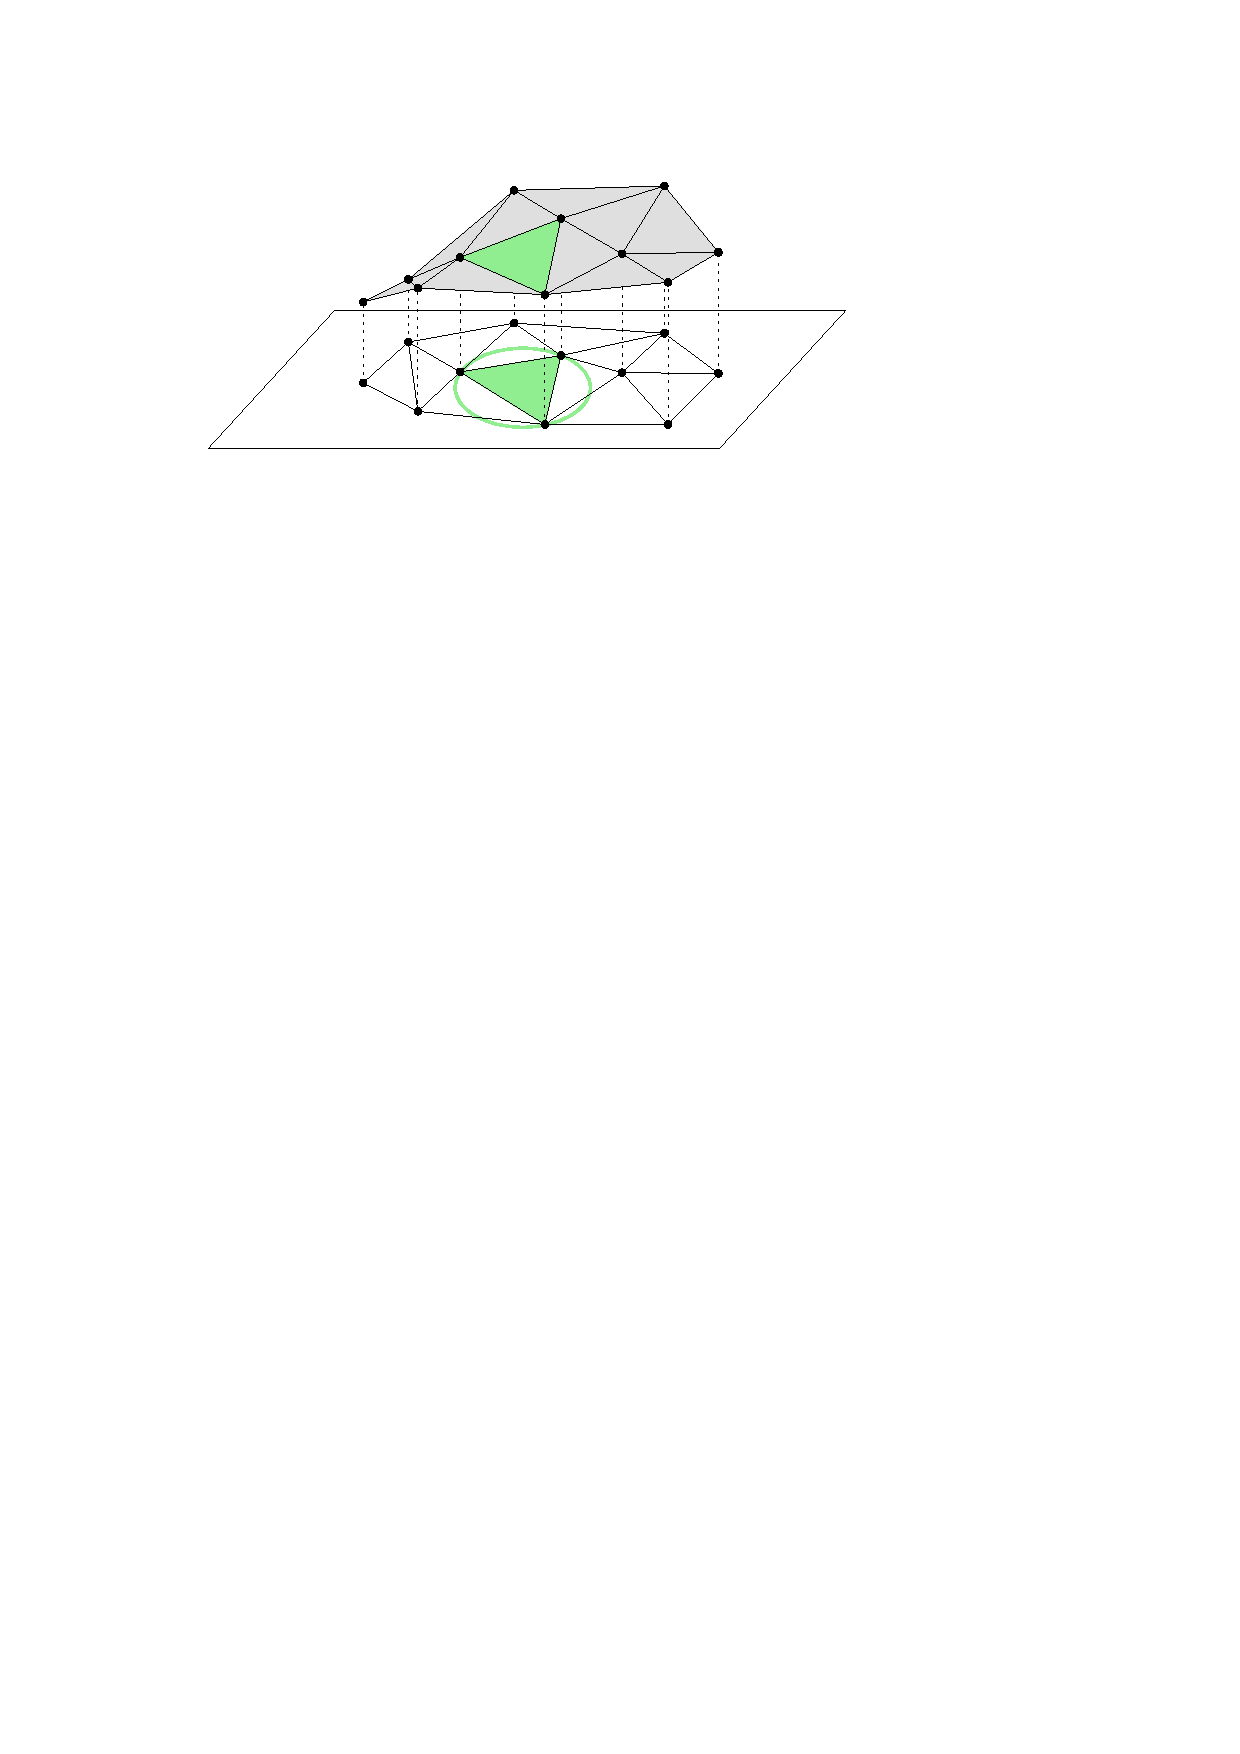
\includegraphics{figs/tin}
  \caption{A TIN is obtained by lifting the vertices to their elevation. All the triangles are usually Delaunay, \ie\ their circumcircle (green) is empty of any other points in the plane.}%
\labfig{fig:tin}
\end{marginfigure}
One way to explain the 2.5D properties of a TIN is as follows: if we project vertically to the $xy$-plane the triangles in 3D space forming the TIN, then no two triangles will intersect.

While not a requirement, the triangulation is usually a Delaunay triangulation (more about this in Chapter~\ref{chap:dtvd}).
The main reason is that Delaunay triangles are as ``fat'' as possible (long and skinny triangles are avoided), and thus they behave better for interpolation.
As can be seen in~\reffig{fig:whydt},
\begin{figure}
  \centering
  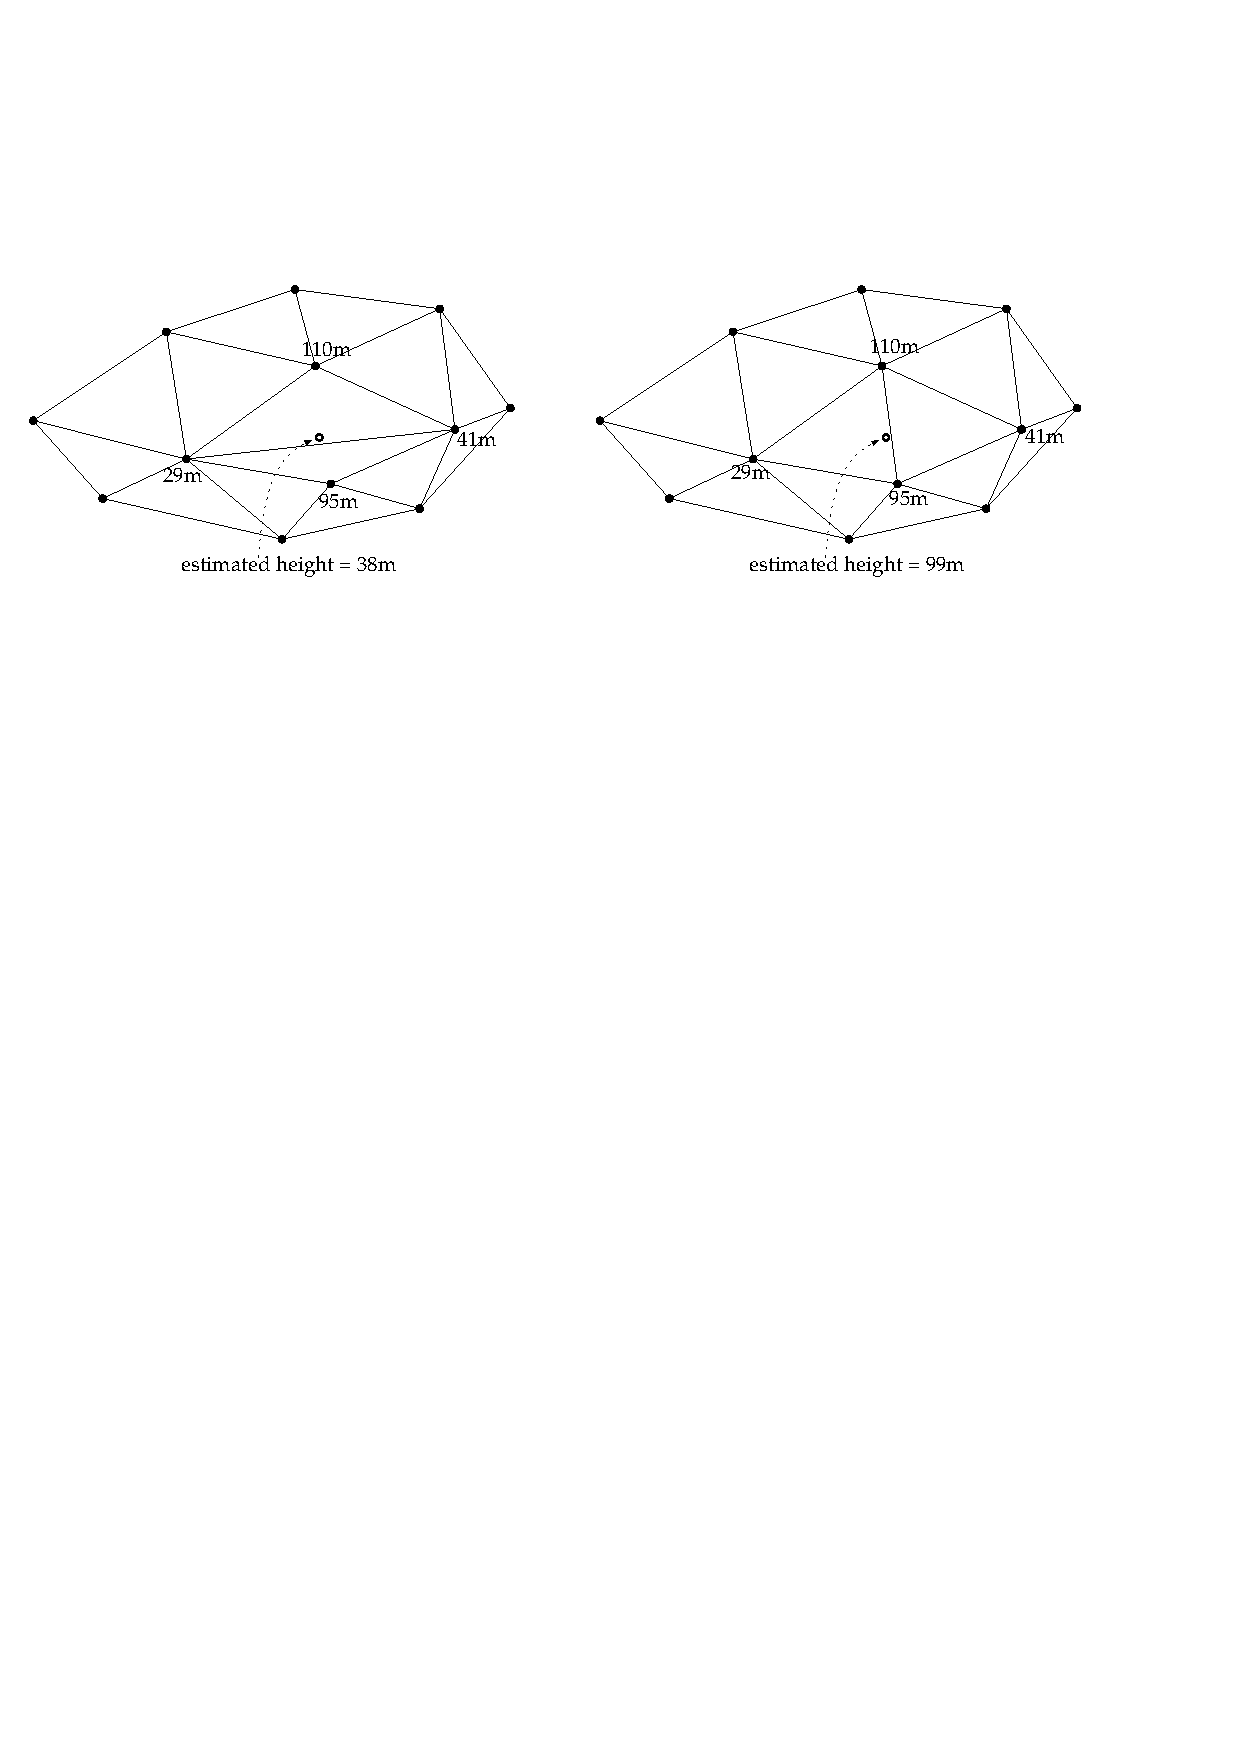
\includegraphics[width=\linewidth]{figs/whydt}
  \caption{Two TINs (left is a DT, right has one non-Delaunay edge) and the result of estimating with linear interpolation in the TIN\@.}%
\labfig{fig:whydt}
\end{figure}
the estimated value can be significantly different, and in this case the right one would make more sense since sample points that are closer to the interpolation location are used (in the TIN on the left, the value of 95m is not used).

%

Each of the points (which becomes vertices in the triangulation) are lifted to its elevation to create a surface, embedded in three dimensions, approximating the morphology of the terrain.
The value of elevation at an unsampled location $p$ is obtained by linearly interpolating on the plane passing through the three vertices of the triangle containing $p$. 
TINs are the most popular alternatives to 2D grids for modelling elevation; both representations have advantages and disadvantages.

%
 
A TIN in which a linear interpolation function is used yields a $C^0$ piecewise representation, \ie\ it is a continuous function but at the edges of the triangles the first derivative is not possible.
It is possible to use higher-order functions in each triangle of a TIN, to construct a $C^1$ or $C^2$ field, \ie\ where the first and second derivative of the surface can be obtained. 



%%%
\subsection{Hierarchical tessellations}

Hierarchical tessellations attempt to reduce the number of cells in a tessellation by merging the neighbouring cells having the same value (thus yielding cells of different sizes).
While both regular and irregular tessellations can be hierarchical, in the context of the representation of terrains, the former is more relevant and is sometimes used in practice.

% Irregular hierarchical tessellations, usually triangulations, are used for obtaining multi-resolution models, or act as a spatial index for efficiently accessing triangles.
% Their use as a support to construct a piecewise function is not necessary because irregular tessellations have cells of different sizes and shapes.
% Consequently, only hierarchical regular tessellations are discussed in the following.

%

A commonly used hierarchical structure in two dimensions is the \emph{quadtree}, which is a generic term for a family of tessellations that recursively subdivide the plane into four quadrants.
As is the case for grids, quadtrees are relatively easily implemented in a computer because they are trees in which each node has exactly four children, if any.

%

The shortcomings of regular hierarchical tessellations are similar to those of regular tessellations: the rotation and scaling operations are difficult to handle.
The main advantage of using them---saving memory space---is present only when there is spatial coherence between cells having the same attribute value, \ie\ when they are clustered together.
Indeed, the size of a quadtree is not dependent on the number of cells, but on their distribution.
The quadtree of a 2D grid having no two adjacent cells with the same value (\eg\ a checkers board) contains the same number of cells as the grid, and its size would most likely be worse because of the overhead to manage the tree.
Another disadvantage is that the notion of neighbours, which is straightforward in regular tessellations, is less trivial.


%%%
\subsection{Other common terrain representations used in GIS}

\begin{marginfigure}
  \centering
  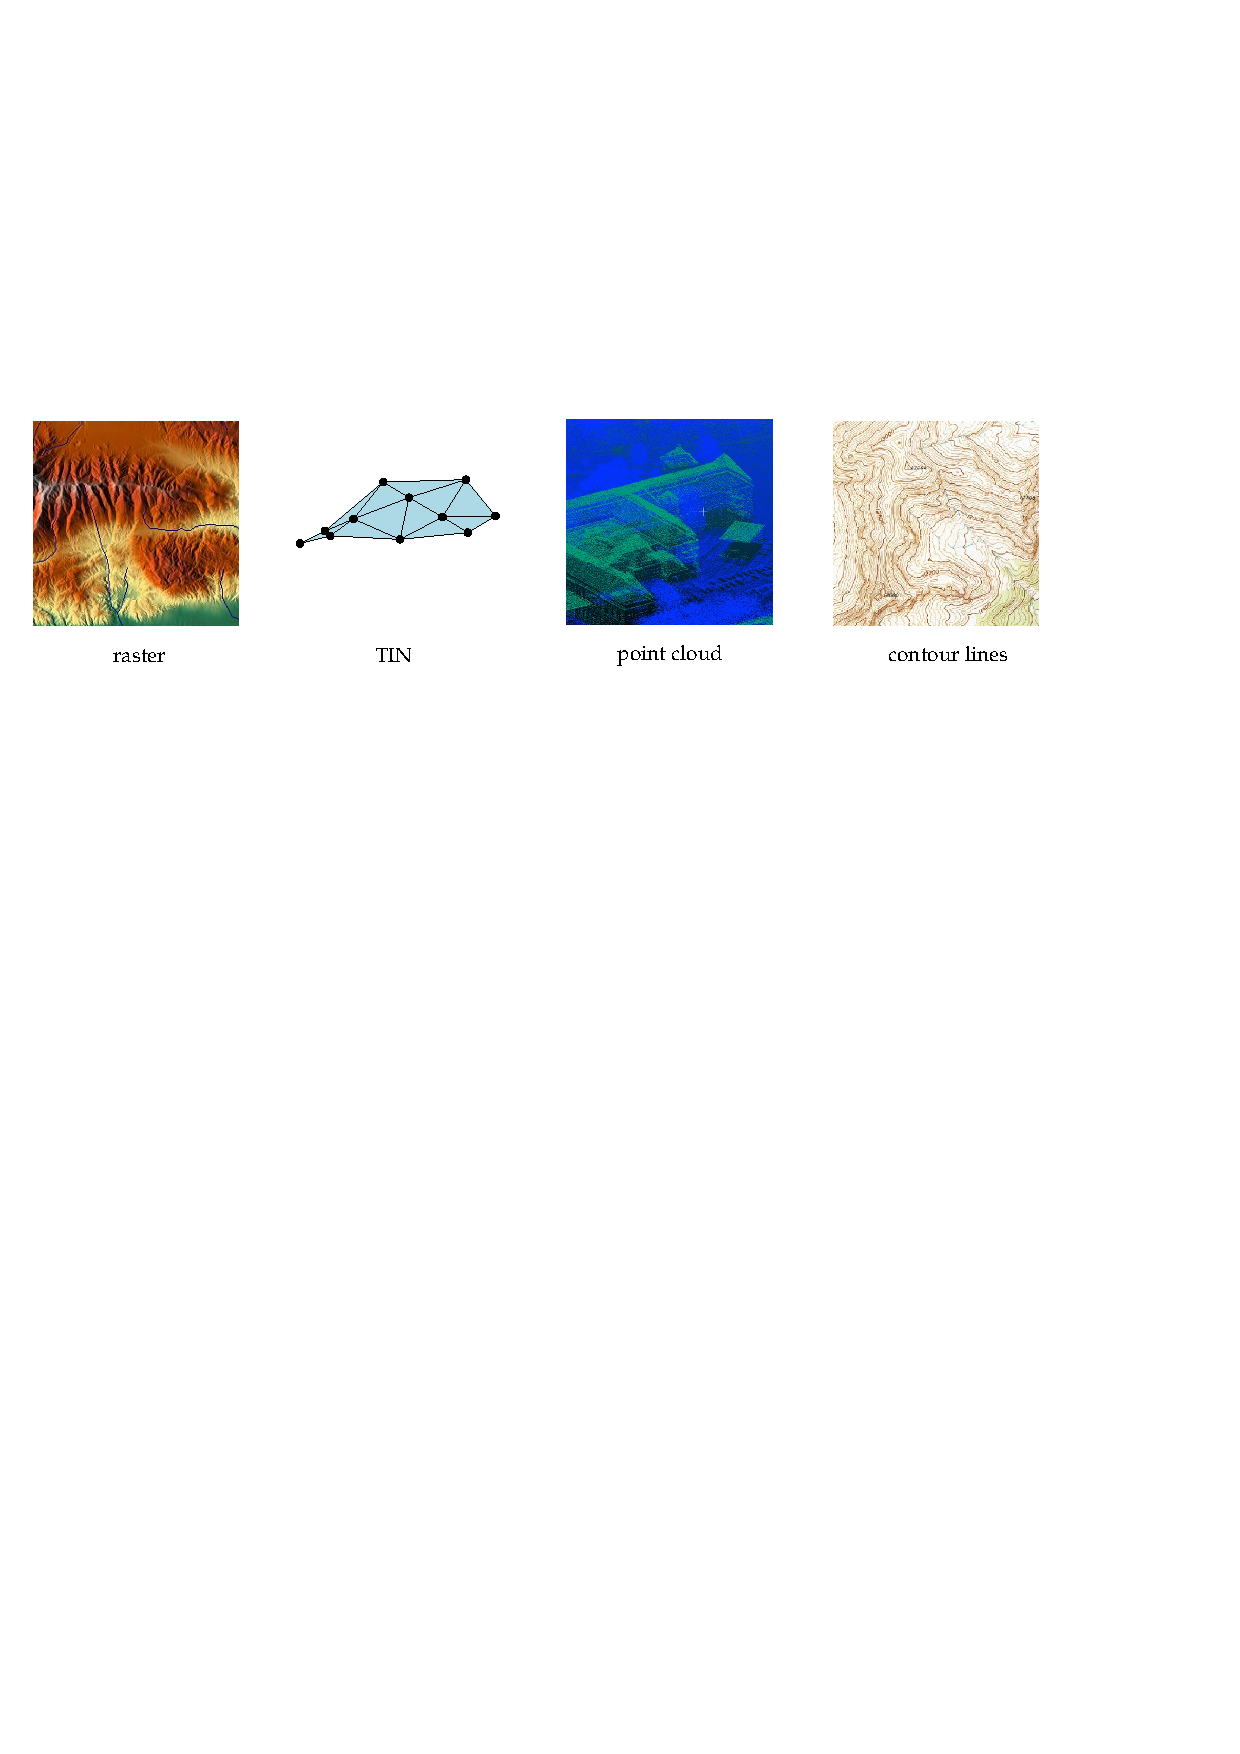
\includegraphics[width=0.75\linewidth]{figs/reps}
  \caption{Four most common data models for terrains.}%
\labfig{fig:reps}
\end{marginfigure}

In the GIS literature, besides the ones above, different representations for terrains are often listed, the two most relevant being:
\begin{enumerate}
  \item irregularly spaced sample points, such a point cloud; 
  \item contour lines.
\end{enumerate}
It should be noticed that these two are however \emph{incomplete}: the set of rules to reconstruct the surface at unsampled locations is not explicitly given, they are not continuous surfaces.
Conceptually speaking, these should therefore not be considered valid representations of a terrain.
While this might seems odd, this is in line with the consensus among practitioners today, where a point cloud or contour lines would typically be used as an input to a process to generate a terrain.

We will nevertheless consider these in the course; the four representations we will use are shown in \reffig{fig:reps}.

%

\paragraph{Contour lines.}

Given a bivariate field $f(x,y) = z$, an \emph{isoline} (commonly named contour line) is the set of points in space where $f(x,y) = z_0$, where $z_0$ is a constant. 
Isolines have been traditionally used to represent the elevation in topographic maps and the depth in bathymetric maps for navigation at sea. 

%

% TODO : change the nicked contour example jpg?
\begin{marginfigure}
  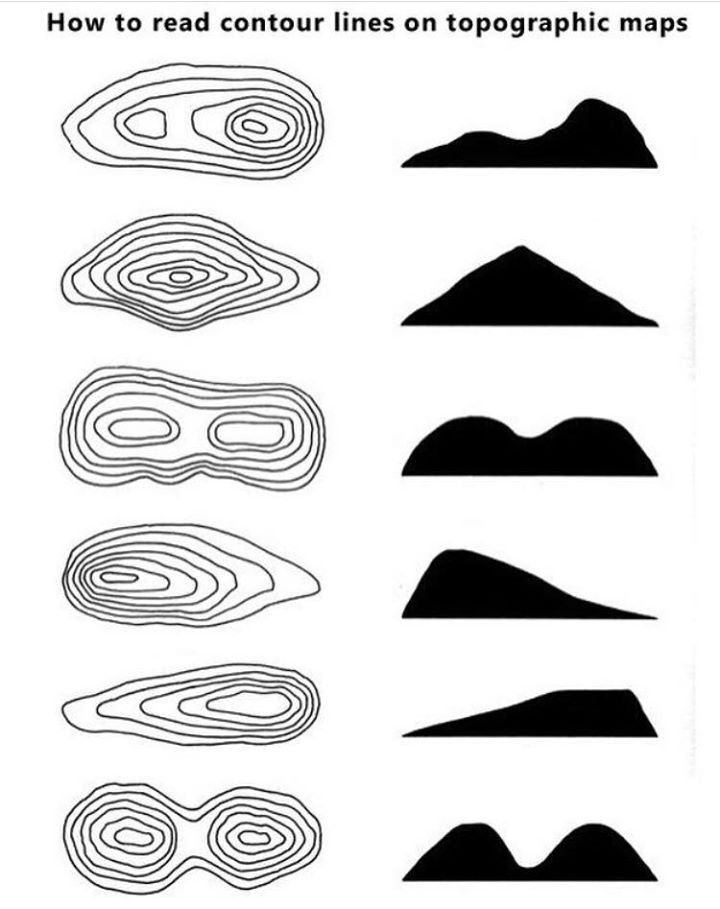
\includegraphics{figs/contours.jpg}
  \caption{A few examples of terrain features and their contour lines. (Figure from \url{https://linguagemgeografica.blogspot.com/})}%
\labfig{fig:contours}
\end{marginfigure}

One particular property of an isoline is that its direction is always perpendicular to the direction of the steepest slope of the terrain. 
Another property that follows from the $2.5D$ property of the field is that contours neither intersect themselves nor each other.

%

The purpose of isolines on a map is to reveal the shape of the underlying terrain. 
By observing the shape and interrelation of neighbouring contours, the presence and significance of surface features becomes apparent; see~\reffig{fig:contours} for a few examples.
It should be noticed that data between contours is absent in the contour map. 
Yet, in case of good contours the reader will still be able to deduct the general morphology of the field. 
It is even so that the use of contours will speed up the map reading process, as it conveys just that relevant bit of data to the map reader rather than `flooding' the reader with information which essentially makes the user do his own cartographic selection. 
Contouring is a form of discretizing the field that makes it easier to use a map. 
Naturally, this comes at a price. 
The level of approximation of the field can (dramatically) differ between contours, the biggest error would be midway in between contour lines. 
But, depending on the relation between the spacing between contours (the \emph{contour interval}) and the map scale, which in turn is dependent on the map application, this effect may be neglected.


%

In practice, isolines are only approximated from the computer representation of a field.
They are usually extracted directly from a TIN or a regular grid. 
As shown in~\reffig{fig:isoline},
\begin{figure}
  \centering
  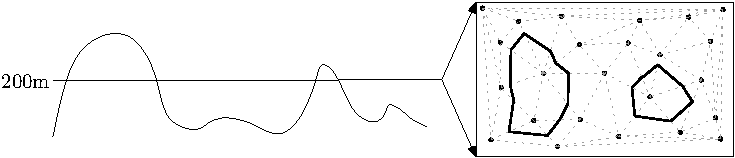
\includegraphics[width=0.95\textwidth]{figs/isoline}
  \caption{Cross-section of a terrain (left), and the 200m isoline extracted from a TIN (right).} 
\labfig{fig:isoline}
\end{figure}
the idea is to compute the intersection between the level value (\eg\ 200m) and the terrain, represented for instance with a TIN\@. 
Each triangle is scanned and segment lines are extracted to form an approximation of an isoline.


%%%
%
\section[TIN versus raster]{TIN versus raster for modelling terrains}

There is an ongoing debate about whether TINs or rasters are the better data model to model terrains.
Practitioners and scientists are probably split 50/50 on the issue.

A data model will be judged more \emph{efficient} than another if it represents a surface more accurately within the same amount of storage space, measured in bytes.
This of course depends on the data structure used to store that data model.

It should be said that both TIN and raster have advantages and disadvantages (as we will see during this course), and in practice one should choose the most appropriate model for the task at hand.
This means converting between the two data models when it is necessary (topic of \refchap{chap:conversion}).


%%%
%
\section{Notes and comments}

\citet{Kumler94} carried out a 4-year comparison between TINs and rasters.
He states that the common belief that a TIN is more space-efficient than raster is handicapped by the fact that a TIN must have \emph{at least} 3 times less points to be of equal space.
His conclusions are also that rasters can estimate elevation more accurately than comparably-sized TINs.
However, he still finishes with by stating: ``Yeah, well\ldots\ TINs still \emph{look} better.'' 

\citet{Fisher97} discusses the disadvantages of rasters, in a GIS and remote sensing context.

\citet{Frank92,Goodchild92a} discuss at lenght the issue of data model, data structure and representation of reality. 

\citet{Tse04} coined the term `2.75D GIS' and show an example of a where a triangulation is used to represent the surface of the Earth, with holes (for tunnels), cliffs and caves. 
The same idea is also referred to as a `2.8D GIS' by \citet{Groger05}.

While more an academic exercise then something used in practice, multi-resolution triangulation have been described and used for some application by \citet{DeFloriani02}.

\citet{Akima78} shows the advantages of using higher-order functions in each region of a TIN, to construct a $C^1$ or $C^2$ field. 

\citet{Dakowicz03} demonstrate that using simple rules (nearest-neighbour for instance) yields fields that are not realistic and have bad slope, which is in practice problematic for several applications.
Obtaining good slope from contour lines is possible, but is in practice a complex process.
% In other words, if elevation is the attribute modelled, the slope of the terrain will be `good', which is important for several applications, for example flood modelling.


%%%
%
\section{Exercises}

\begin{enumerate}
  \item Explain in our own words why a point cloud (\eg\ collected with airborne lidar) is not considered a complete representation of a terrain.
  \item What is a bivariate function? 
  \item Assume you have 2.75D terrain of an area. Is it possible to extract the isolines from it? What properties will these have? Will they intersect?
\end{enumerate}
 %- 01
%!TEX root = ../terrainbook.tex
% chktex-file 46


\setchapterpreamble[u]{\margintoc}

\graphicspath{{acquisition/}}


\chapter{Acquisition of elevation measurements}%
\label{chap:acquisition}

The very first step in the process of terrain modelling is the acquisition of elevation measurements. 
Nowadays, these measurements are usually collected in large quantities using some form of remote sensing, \ie\ sensors that measure---in our case---the distance to the Earth's surface from an airborne or even a spaceborne platform. 
In raw form, elevation measurements are typically stored as a point cloud, \ie\ a collection of georeferenced 3D points with each point representing one elevation measurement on the Earth's surface.

There are a number of remote sensing techniques that are used to measure elevation on Earth or other planets. 
Typically, these techniques measure
\begin{enumerate}
	\item the distance to the target surface; 
	\item their own position and orientation with respect to some global reference system. 
\end{enumerate}
By combining these, we can compute the 3D coordinates of the measured location on the target surface. 

In this chapter we will focus primarily on lidar, the most common acquisition technique for large scale terrain models with centimetre level accuracy. 
But we also give an overview of other acquisition techniques, for example photogrammetry, InSAR, and sonar. 
And to conclude we will look at typical artefacts that you might encounter while working with elevation data. 
This is because, as with any kind of real-world measurements, there are various uncertainties and restrictions in the acquisition process that lead to distortions---the \emph{artefacts}---in the acquired data. These artefacts need to be taken into account when further processing and using the elevation data. 
%This often makes further processing of the data more difficult, because these artefacts often violate assumption that are made in the DTM algorithms used to further process and analyse the point cloud, leading to erroneous results. 
% It is important that you are aware of these artefacts while working with elevation data, because only then you will be able to make the right modelling decisions. 
%Section~\ref{sec:artefacts} gives an overview of common problems in elevation data.

\section{Principles of lidar}%
\label{sec:lidar-principles}\index{lidar}

A lidar system\sidenote{While `lidar' is often treated as the acronym of \textbf{li}ght \textbf{d}etection \textbf{a}nd \textbf{r}anging, it actually originated as a portmanteau of `light' and `radar'. (from \href{https://en.wikipedia.org/wiki/Lidar\#History\_and\_etymology}{Wikipedia})} measures the distance to a target by illuminating it with pulsed laser light and measuring the reflected or \emph{backscattered}\sidenote{Backscattering is the natural phenomenon of  the reflection of (electromagnetic) waves or signals back to the direction they came from.} signal with a sensor (see Figure~\ref{fig:acqLidar}). 
\begin{marginfigure}
	\centering
	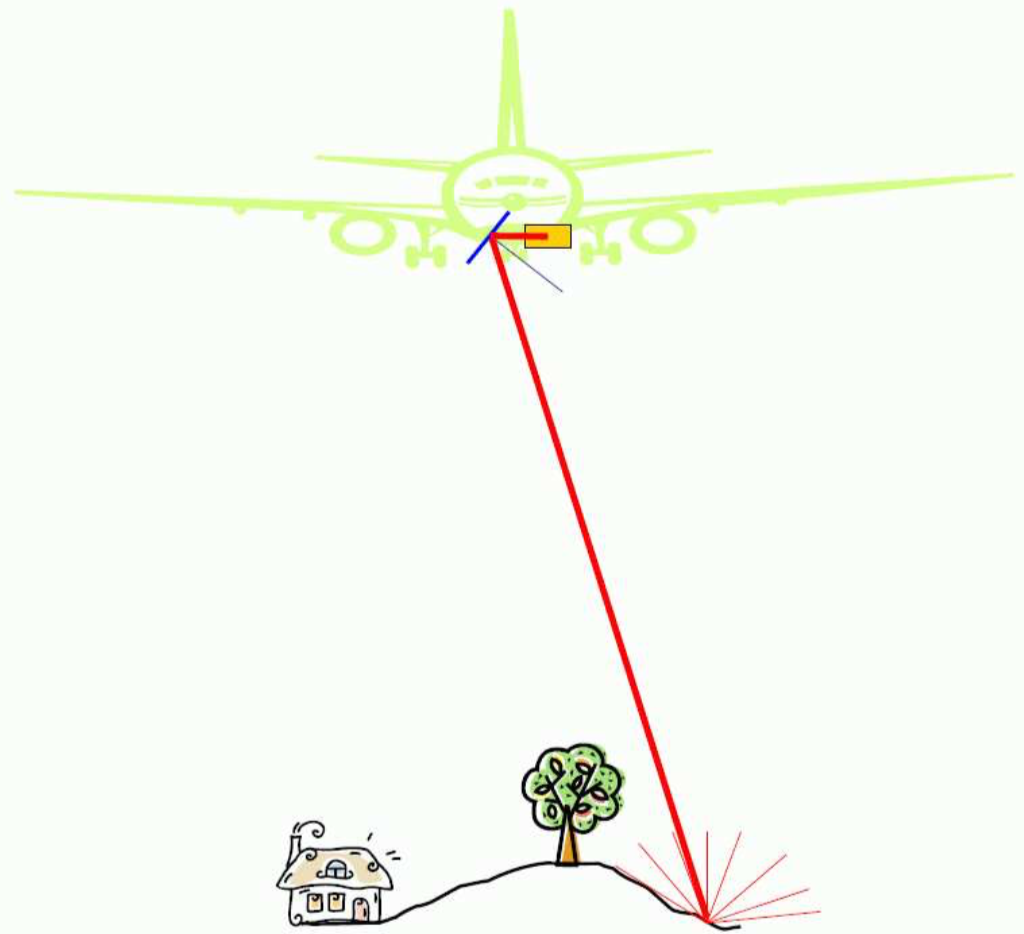
\includegraphics[width=\textwidth]{figs/lidar.png}
	\caption{Lidar range measurement}%
	\label{fig:acqLidar}
\end{marginfigure}
By measuring the time-of-flight, \ie\ the difference in time between emitting a pulse and detecting its return or \emph{echo}, the distance to the target that reflected the pulse can be found using a simple formula. To be exact, the time-of-flight $T$ is equal to
\begin{equation}
	\label{eq:tof}
	T= 2 \frac{R}{c}
\end{equation}
where $c$ is the speed of  light (approximately 300,000 km/s), and $R$ is the distance or \emph{range} between the lidar scanner and the target object that reflects the laser pulse. Therefore the range $R$ can be found from the measured time-of-flight $T$ using
\begin{equation*}
	R = \frac{1}{2} Tc.
\end{equation*}
A typical lidar systems performs hundreds of thousands of such range measurements per second. 

Lidar scanners exist in various forms. 
They can be mounted on a static tripod (terrestrial lidar) for detailed local scans, or on a moving platform such as a car (mobile lidar) or an aircraft (airborne lidar) for rapid scanning of larger areas. Nowadays, also hand-held lidar systems exist, and even some of the latest smartphones  have a lidar sensor. 
Furthermore, lidar can also be used from a satellite in space\sidenote{NASA has used space lidar \href{https://en.wikipedia.org/wiki/ICESat-2}{on Earth}, \href{https://lola.gsfc.nasa.gov}{on the Moon}, and \href{https://en.wikipedia.org/wiki/Mars_Orbiter_Laser_Altimeter}{on Mars}.}. 

However, in the remainder of this text we will focus on airborne lidar.


%%%
%
\subsection{Georeferencing the range measurements}

\begin{figure}
	\centering
	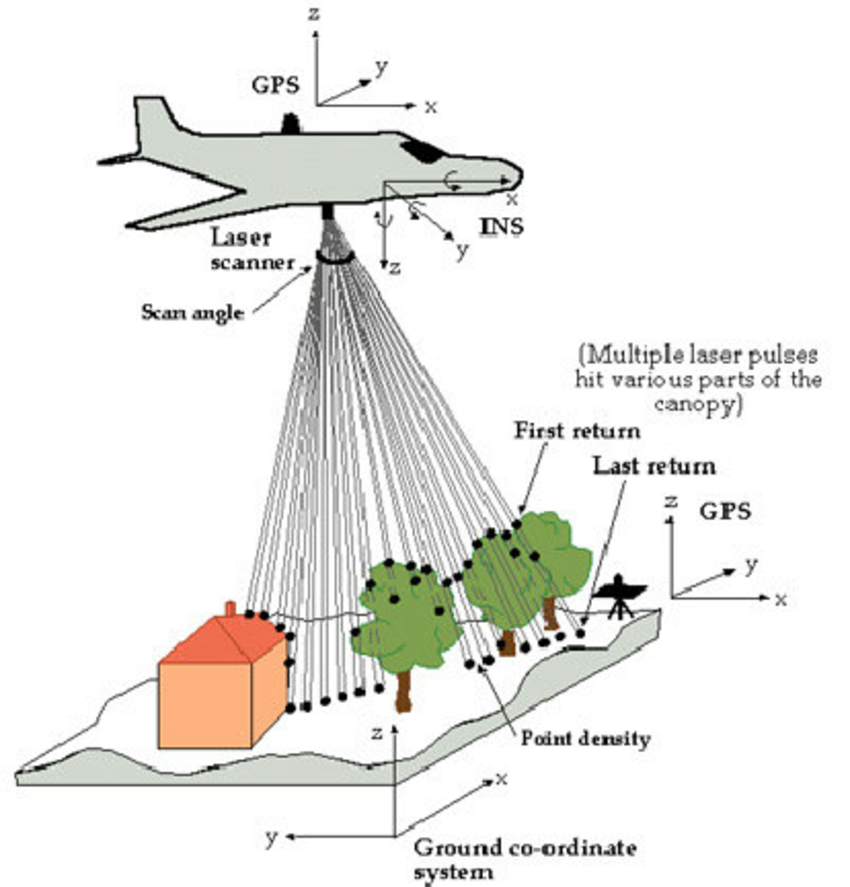
\includegraphics[width=0.7\textwidth]{figs/lidar-gnss-imu.png}
	\caption{An airborne lidar system. Figure from \citet{Dowman04}.}%
\label{fig:airborne-lidar}
\end{figure}
Apart from the  laser scanner itself, a lidar  system uses a GPS receiver and an inertial navigation system (INS), see Figure~\ref{fig:airborne-lidar}. 
\marginnote{inertial navigation system (INS)}\index{inertial navigation system (INS)}
These devices, which respectively provide the global position and orientation of the laser scanner, are needed for georeferencing, \ie\ to convert the range measurements of the laser scanner to 3D point measurements in a global coordinate system such as WGS84. 

To  obtain an accurate global position, \emph{differential GPS} (DGPS) is employed. 
\marginnote{differential GPS}\index{differential GPS}
DGPS is a technique to enhance the accuracy of GPS  by using GPS stations on the ground (one is visible in Figure~\ref{fig:airborne-lidar}). 
These DGPS stations have a known position and they broadcast the difference between that  known position and the position at the station as indicated by GPS\@. 
This difference is essentially a correction for errors in the GPS signal. The aircraft receives these differences from nearby DGPS stations and uses them to correct the GPS position of the aircraft. Using DGPS the accuracy of the GPS position on the aircraft can be improved from around 15 meters to several centimetres.

To obtain the accurate orientation of the laser scanner, the INS of the aircraft is used. 
The INS accurately measures the orientation, \ie\ the yaw, pitch  and roll angles of the aircraft, by means of an inertial measurement unit (IMU)\sidenote{\url{https://en.wikipedia.org/wiki/Inertial_measurement_unit}}. 
\marginnote{inertial measurement unit (IMU)}\index{inertial measurement unit (IMU)}
Only when we accurately know the orientation of the laser scanner, can we know the direction (in a global coordinate system) in which a laser pulse is emitted from the aircraft.

By combining the global position and the global orientation of the laser scanner with the range measurement from the laser scanner, the georeferenced 3D position of  the point  on the target object that reflected the lase pulse can be computed.


%%%
\subsection{Echo detection}

A lidar system performs ranging measurements using the time-of-flight principle that allows us to compute range from a time measurement using the known speed of light in the air. 
The time measurement starts when the laser pulse is emitted and is completed when a backscattered echo of that signal is detected. 
In practice one emitted pulse can even lead to multiple echoes  in the case when an object reflects part of the laser pulse, but also allows part of the pulse to continue past the object. 
Notice that lidar pulses are typically emitted in a slightly divergent manner. As a result the footprint of the pules at ground level is several centimetres in diameter, which increases the likelihood of multiple echoes.

\begin{figure}
	\centering
	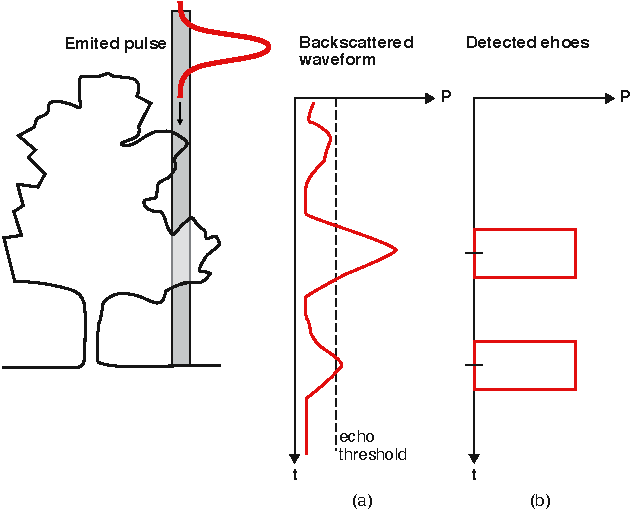
\includegraphics[width=0.8\textwidth]{figs/lidar-multipulse.pdf}
	\caption{The emitted laser pulse, \textbf{(a)} the returned signal, and \textbf{(b)} the recorded echoes. Figure adapted from \citet{Bailly12}.}%
\label{fig:lidar-multipulse}
\end{figure}
Figure~\ref{fig:lidar-multipulse} illustrates what the backscattered signal looks like when it hits a target object in the shape of a tree. 
A tree is particularly interesting because it often causes multiple echoes (one or more on its branches and one on the ground below).  The lidar sensor observes a waveform that represents the received signal power ($P$) as a function of time ($t$). 
With the direct detection lidar systems that we focus on in this book, the echoes are derived from the backscattered waveform by using a thresholding technique. This essentially means that an echo is recorded whenever the power of the waveform exceeds a fixed threshold (see Figure~\ref{fig:lidar-multipulse}b). 

An echo can  also  be referred to as a \emph{return}. 
\marginnote{return}\index{return}
For each return the return count is recorded, \eg\ the first return is the first echo received from an emitted laser pules and the last return is the last received echo (see Figure~\ref{fig:lidar-multipulse}). The return count can in some cases be used to determine if an echo was reflected on vegetation or ground (ground should then be the last return).


%%%
\subsection{Anatomy of a lidar system}%
\label{lidar:anatomy}


A lidar system consists of an optical and an electronic part. 
As shown in Figure~\ref{fig:lidar-components}, each part consists of several components.
\begin{figure}
	\centering
	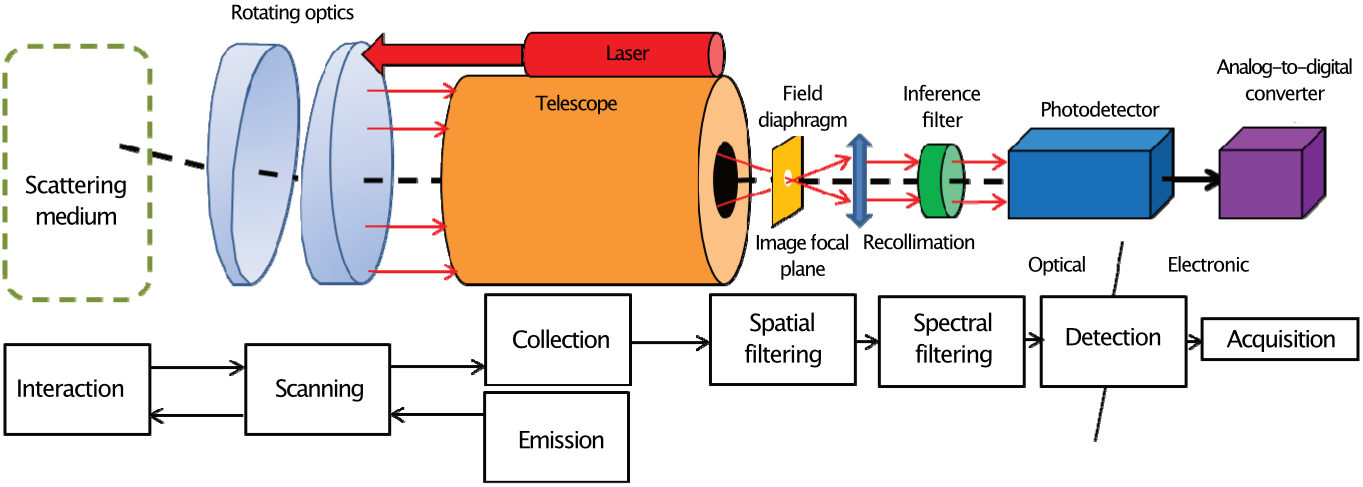
\includegraphics[width=\textwidth]{figs/lidar-components.png}
	\caption{Conventional architecture of a direct detection lidar system. Figure from \citet{Chazette16}.}%
\label{fig:lidar-components}
\end{figure}

In the optical part, a pulse of a particular wavelength (typically near-infrared) is generated by the laser source for each lidar measurement. 
It then passes through a set of  optics (lenses and mirrors) so that it leaves the scanner in an appropriate direction. 
After the pulse interacts with the scattering medium, it is reflected back into the scanning optics which then directs the signal into a telescope. 
The telescope converges the signal through a field diaphragm (essentially a tiny hole around the point of convergence). 
The field diaphragm blocks stray light rays (\eg\ sunlight reflected into the optics from any angle) from proceeding in the optical pipeline. 
Next, the light signal is recollimated so that it again consists only of parallel light rays. 
The final step of the optical part is the inference filter which blocks all wavelengths except for the wavelength of the laser source. 
This is again needed to block stray light rays from distorting the measurement.

The electronic part consists of a photodetector, which first transforms the light signal into an electrical current, which is then converted to a digital signal using the analogue-to-digital converter. 
Once the digital signal is available, further electronics can be used to interpret and record the signal.


%%%
\subsection{Laser wavelength}

Choosing the optimal laser wavelength is a compromise of several different factors. 
One needs to consider atmospheric scattering, 
\marginnote{atmospheric scattering}\index{atmospheric scattering}
\ie\ how much of the signal is lost simply by travelling through the atmosphere, and the absorption capacity of vegetation, \ie\ how much of  the signal is lost because it is absorbed by vegetation. In addition, there is the stray signal due to direct and scattered contributions of sunlight. While it is possible to filter such stray signals in the lidar system to some degree, it remains wise to choose a wavelength that is only minimally affected by it. Finally there are regulations that limit the laser radiance values permissible to the eye. This means that the power of emitted signal needs to be carefully controlled, and/or a wavelength must be chosen that  is not absorbed by the eye so much.

As a result, most lidar systems use a wavelength in the near-infrared spectrum, usually between 600 and 1000 nm. A notable exception is made for bathymetric purposes, in which case a green (532 nm) laser is used because that has a greater penetration ability in water.

\subsection{Scanning patterns}
In order to improve the capacity to quickly scan large areas, a number of rotating optical elements are typically present in a lidar system. Using these optical elements, \ie\  mirrors or prisms, the emitted laser pulse is guided in a cross-track direction (\ie\ perpendicular to the along-track direction in which  the aircraft moves, see Figure~\ref{fig:acqLidar}),  thereby greatly increasing the scanned ground area  per travelled meter of the aircraft.
Figure~\ref{fig:lidar-patterns} depicts a number of possible configurations of rotating optics and shows the resulting scanning patterns. It is clear that density of points on the ground is affected by the scanning pattern. The top example for example, yields much higher densities on edges of the scanned area. In practice more uniform patterns, such  as the bottom two examples are often preferred.

\begin{figure}
	\centering
	\includegraphics[width=0.7\textwidth]{figs/lidar-patterns.pdf}
	\caption{Different configurations of rotating mirrors and the associated scanning patterns from a moving platform. Arrows indicate the direction of the emitted laser signal. Figure from \citet{Chazette16}.}%
\label{fig:lidar-patterns}
\end{figure}



\begin{kaobox-toread}[frametitle=\faExternalLink\ To read or to watch]
	This YouTube video explains the principles of an aerial LiDAR system:
	\\
	\url{https://youtu.be/EYbhNSUnIdU}
\end{kaobox-toread}


% TODO : put a side-by-side with vegetation and without lidar to show DTM and DSM


\section{Other acquisition techniques}%
\label{sec:acquisistion-techniques}

Apart from lidar there are also other sensor techniques that can be used to acquire elevation data. Some of these are  active sensors just like lidar (a signal is generated and emitted from the sensor), whereas others are passive (using the sun as light source). And like lidar, these sensors themselves only do range measurements, and need additional hardware such as a GPS receiver and an IMU to georeference the measurements. What follows is a brief description of the three other important acquisition techniques used in practice. 

% FIXME image with flight parameters and strips

\subsection{Photogrammetry}%
\label{sec:photogrammetry}\index{photogrammetry}
\begin{marginfigure}
	\centering
	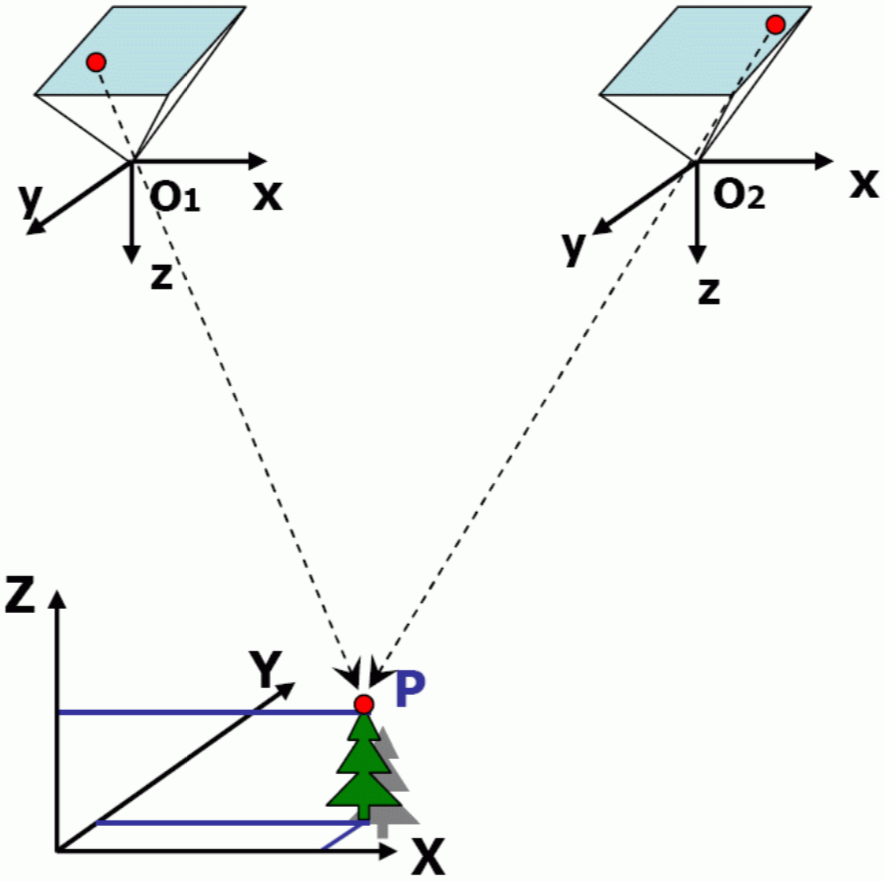
\includegraphics[width=\textwidth]{figs/photogrammetry.png}
	\caption{Photogrammetry}%
	\label{fig:acqPhoto}
\end{marginfigure}
Photogrammetry allows us to measure the distance from overlapping photographs taken from different positions. 
If a ground point, called a \emph{feature}, is identifiable in two or more images, its 3D coordinates can be computed in two steps. 
First, a viewing ray for that feature must be reconstructed for each image. 
A viewing ray can be defined as the line from the feature, passing through the projective centre of the camera, to the corresponding pixel in the image sensor (see Figure~\ref{fig:acqPhoto}). 
Second, considering that we know the orientation and position of the camera, the distance to the feature (and its coordinates) can be computed by calculating the spatial intersection of several viewing rays.

% interior orientation (camera parameters such as focal length) and the exterior orientation (camera position and orientation)

The number of 3D point measurements resulting from photogrammetry thus depends on the number of features that are visible in multiple images, \ie\ the so-called matches.
With \emph{dense image matching} 
\marginnote{dense image matching}\index{dense image matching}
it is attempted to find a match for every pixel in an image. 
If the ground sampling distance, \ie\ the pixel size on ground level, is small (around \SI{5}{\cm} for state-of-the-art systems), point densities of hundreds of points per square meter can be achieved, which is much higher than the typical lidar point cloud (typically up to dozens of points per square meter). 

In photogrammetry we distinguish between \emph{nadir} images, 
\marginnote{nadir images}\index{nadir images}
that are taken in a direction straight down from the camera, and \emph{oblique}
\marginnote{oblique images}\index{oblique images}
images that are taken at an angle with respect to the nadir direction.
Vertical features such as building façades are only visible on oblique images.
Therefore, oblique images are needed if one wants to see building façades in a dense image matching point cloud.

Because photography is used, photogrammetry gives us also the colour of the target surface, in addition to the elevation.
This could be considered an advantage over lidar which captures several attributes for each point (\eg\ the intensity of measured laser pulse and the exact GPS time of measurement), but colour is not among them.

Both airborne and spaceborne photogrammetry are possible.

%%%
\subsection{InSAR}%
\label{sec:insar}%
\index{InSar}

Interferometric synthetic aperture radar (InSAR) is a radar-based technique that is used from space in the context of terrain generation. 
It is quite different from airborne lidar or photo\-gramme\-try-based acquisition because of the extremely high altitude of the satellite carrying the sensor. 
Signals have to travel very long distances through several layers of unpredictable atmospheric conditions. 
As a result the speed of the radar signal is not known and the time-of-flight principle can not be used to get detailed measurements. 
However, by using a comprehensive chain of processing operations based on the measured phase shifts and the combination of multiple InSAR images, accurate elevation can still be measured. 
With InSAR it is possible to cover very large regions in a short amount of time, \eg\ the global SRTM\sidenote{\url{https://en.wikipedia.org/wiki/Shuttle_Radar_Topography_Mission}} dataset was generated with InSAR\@. 
Compared to dense image matching and lidar, InSAR-derived DTMs usually have a much lower resolution, \eg\ SRTM has a pixel size of 30 meters.

%%
\begin{kaobox-toread}[frametitle=\faExternalLink\ To read or to watch]
	\href{https://en.wikipedia.org/wiki/Interferometric_synthetic-aperture_radar}{Wikipedia page about \emph{Interferometric synthetic-aperture radar}}.
\end{kaobox-toread}


%%%
\subsection{Echo sounding}%
\label{sec:mbes}
Echo sounding is a form of sonar that can be used for bathymetry, \ie\ mapping underwater terrains from a boat. 
Similar to lidar, it uses the time-of-flight principle to compute distance, but sound is used instead of light. 

Single-beam and multi-beam echo sounders exist. Multi-beam systems are capable of receiving many narrow sound beams from one emitted pulse. As a result it measures the target surface much more accurately. 
For bathymetry usually a multi-beam echo sounder is used.

Chapter~\ref{chap:bathymetry} describes techniques to process bathymetric datasets and create terrain of the seabed.

%%
\begin{kaobox-toread}[frametitle=\faExternalLink\ To read or to watch]
  The principles of echo sounding.
  \\
  \url{https://en.wikipedia.org/wiki/Echo_sounding}
\end{kaobox-toread}




\section{Artefacts}%
\label{sec:artefacts}

In the acquisition process, there are many aspects---both under our control and not under our control--- that affect the quality and usability of the resulting elevation data for a given application. 
Some examples are
\begin{itemize}
	\item the choice of the sensor technique, 
	\item the sensor specifications, \eg\ the resolution and focal length of a camera, or the scanning speed, the width of the swath, and scanning pattern of a lidar system,
	\item the flight parameters, \eg\ the flying altitude and the distance and overlap between adjacent flights,
	\item atmospheric conditions, 
	\item the physical properties of the target surface.
\end{itemize}

An artefact is any error in the perception or representation of information that is introduced by the involved equipment or techniques. 
Artefacts can result in areas without any measurements (\eg\ the \emph{no-data} values in a raster), or in so-called \emph{outliers}, \ie\ sample points with large errors in their coordinates. 
\marginnote{outliers}\index{outliers}

We distinguish three types of artefacts, 
\begin{enumerate}
	\item those that occur due to problems in the sensor, 
	\item those that occur due to the geometry and material properties of the target surface, 
	\item those that occur due to post-processing steps.
\end{enumerate}

% Active/passive sensors
% different platforms ground/airborne/space
% different physical principles
% pulse footprint, wavelength
% different sensor specs (resolution, speed) and operation specs (flight height etc)
% different cost, update cycles

\subsection{Sensor orientation}
The sensor position and orientation are continuously monitored during acquisition, \eg\  by means of GNSS and an IMU for airborne and seaborne systems, and used to determine the 3D coordinates of the measured points. 
Consequently, any errors in the position and orientation of the sensor platform affect the elevation measurements. 
For this reason adjacent flight strips (see Figure~\ref{fig:lidarStrips}) often need to be adjusted to match with each other using ground control points. 
\begin{figure}
	\centering
	\begin{subfigure}{0.4\linewidth}
		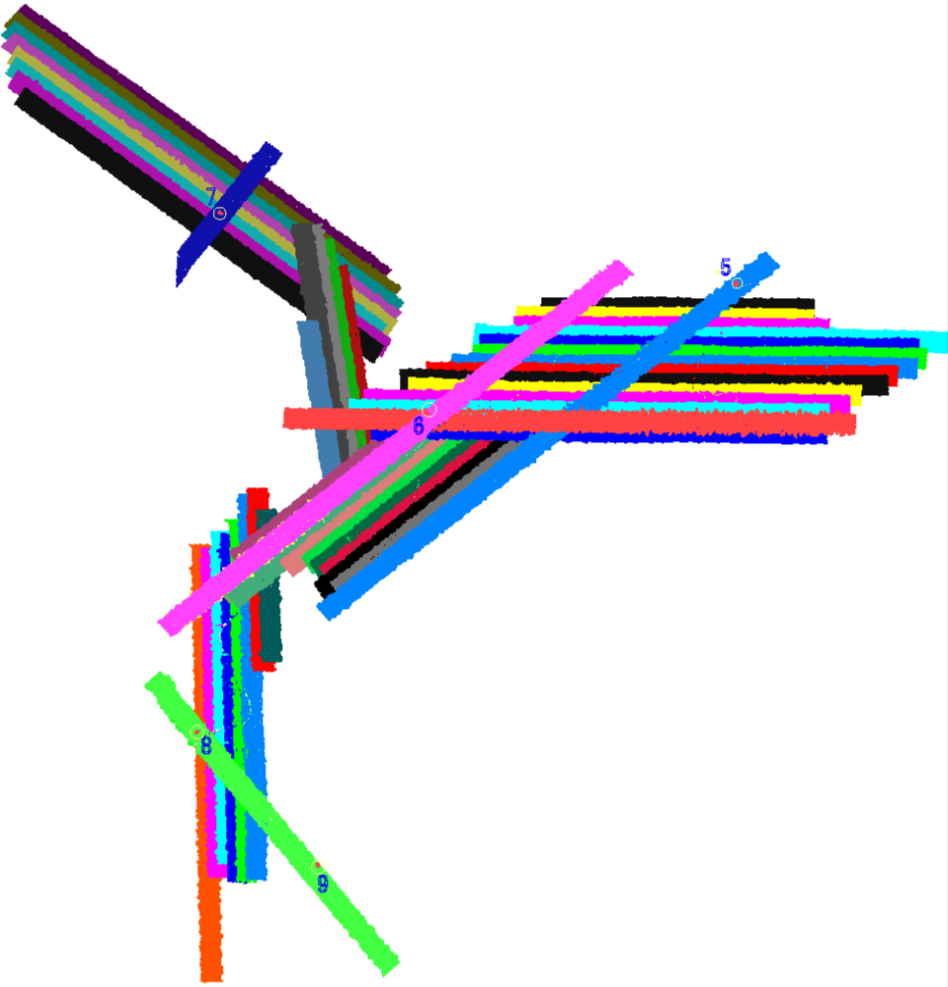
\includegraphics[width=\textwidth]{figs/lidar_strips.png}
		\subcaption{Plan view of the different strips of a lidar survey \citep{Kornus03}}\label{fig:lidarStrips}
	\end{subfigure}
	\quad
	\begin{subfigure}{0.4\linewidth}
		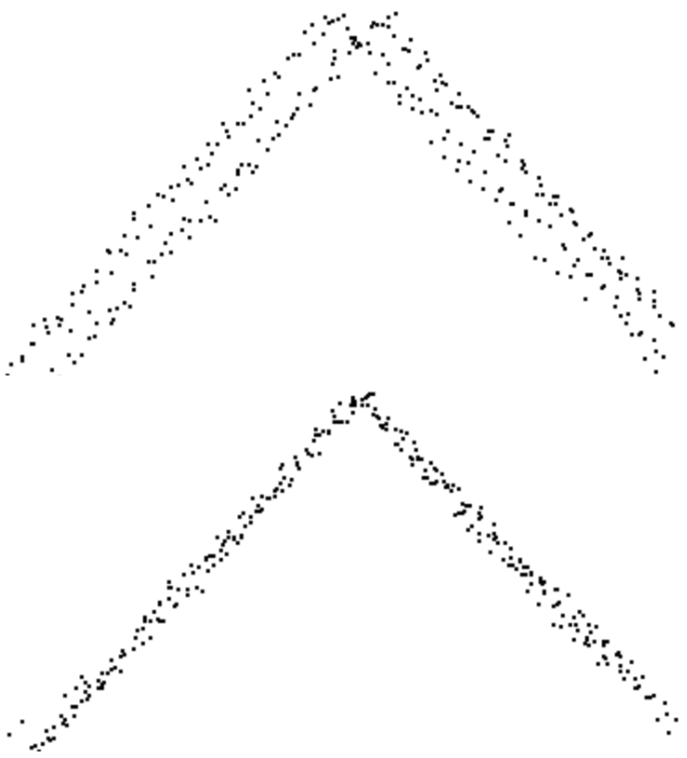
\includegraphics[width=\textwidth]{figs/strip_adjustment.png}
		\subcaption{Cross-section of gable roof before (top) and after (bottom) strip adjustment \citep{Vosselman02}}\label{fig:lidarGableRoof}
	\end{subfigure}
	\caption{Strip adjustment for lidar point clouds}%
\label{fig:lidarStripAdj}
\end{figure}
If the strip adjustments process fails or is omitted, a `ghosting' effect can occur as illustrated in Figure~\ref{fig:lidarGableRoof} (top). 
Photogrammetry knows a similar process called aerial triangulation, in which camera positions and orientation parameters (one set for each image) are adjusted to fit with each other. Errors in the aerial triangulation can lead to a noisy result for the dense matching as seen in Figure~\ref{fig:dim}.
\begin{figure*}
	\centering
	\begin{subfigure}{0.45\linewidth}
		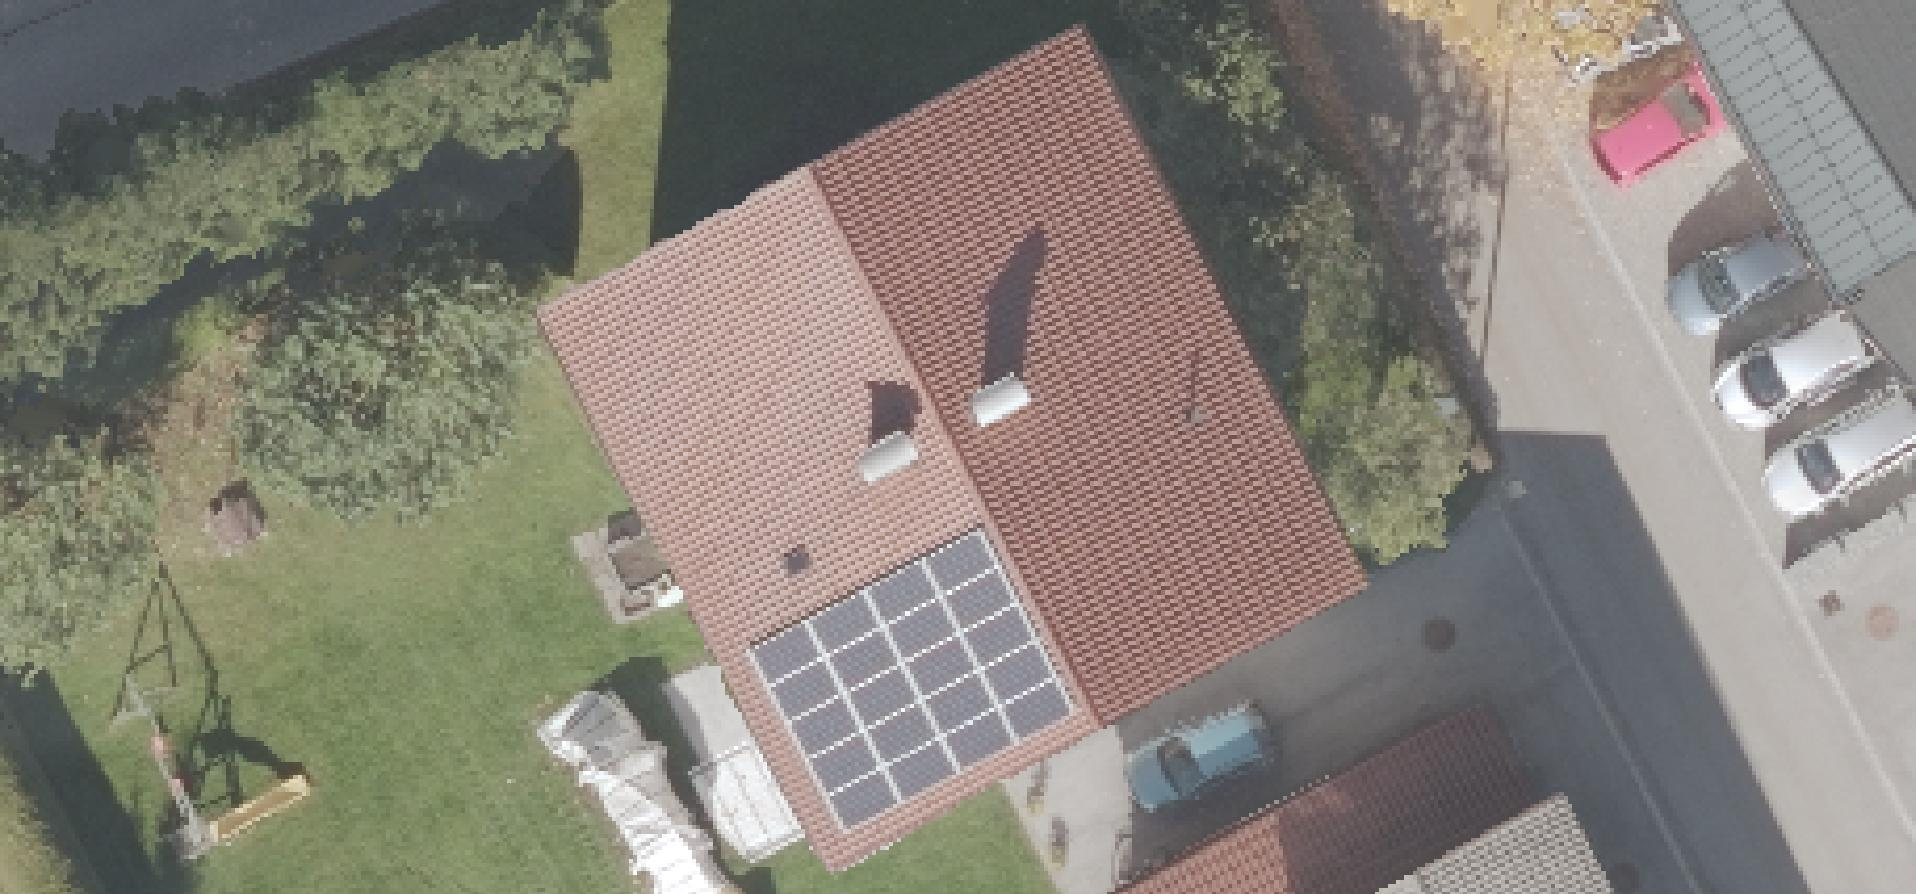
\includegraphics[width=\textwidth]{figs/Roof_OP_NA_10cm.jpg}
		\subcaption{Nadir image}\label{fig:dim:a}
	\end{subfigure}
	
	\begin{subfigure}{0.45\linewidth}
		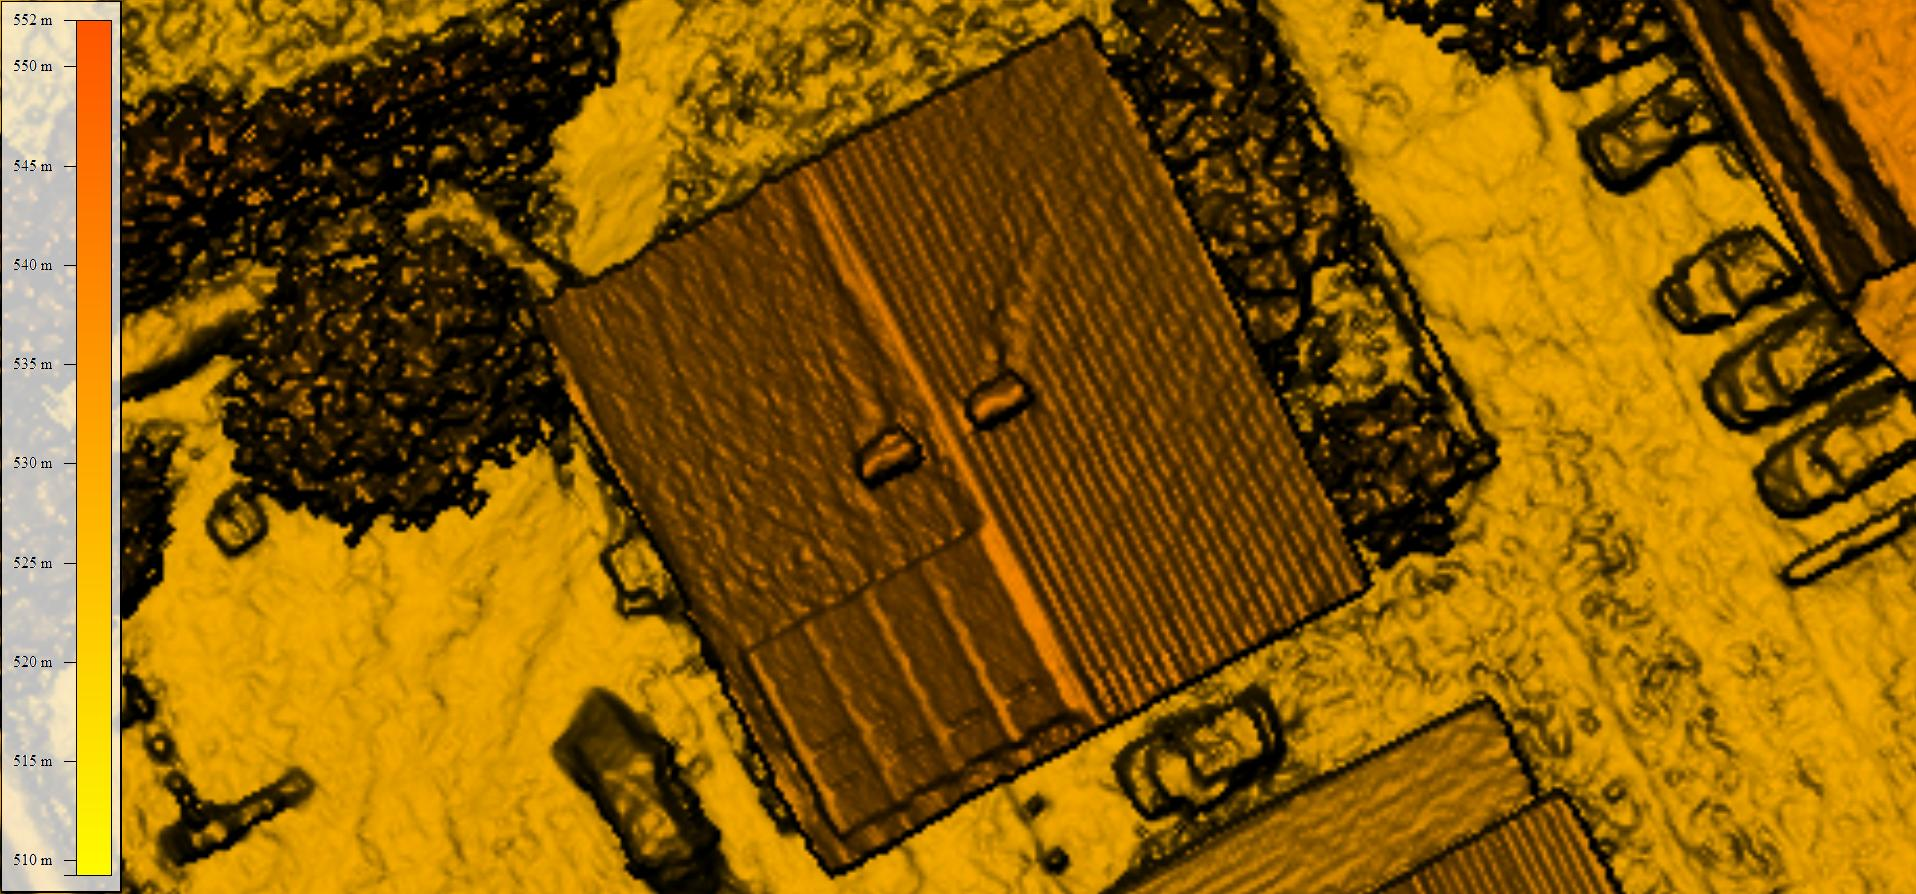
\includegraphics[width=\textwidth]{figs/Roof_DSM_NA_10cm.jpg}
		\subcaption{DSM with good aerial triangulation}\label{fig:dim:b}
	\end{subfigure}
	\quad
	\begin{subfigure}{0.45\linewidth}
		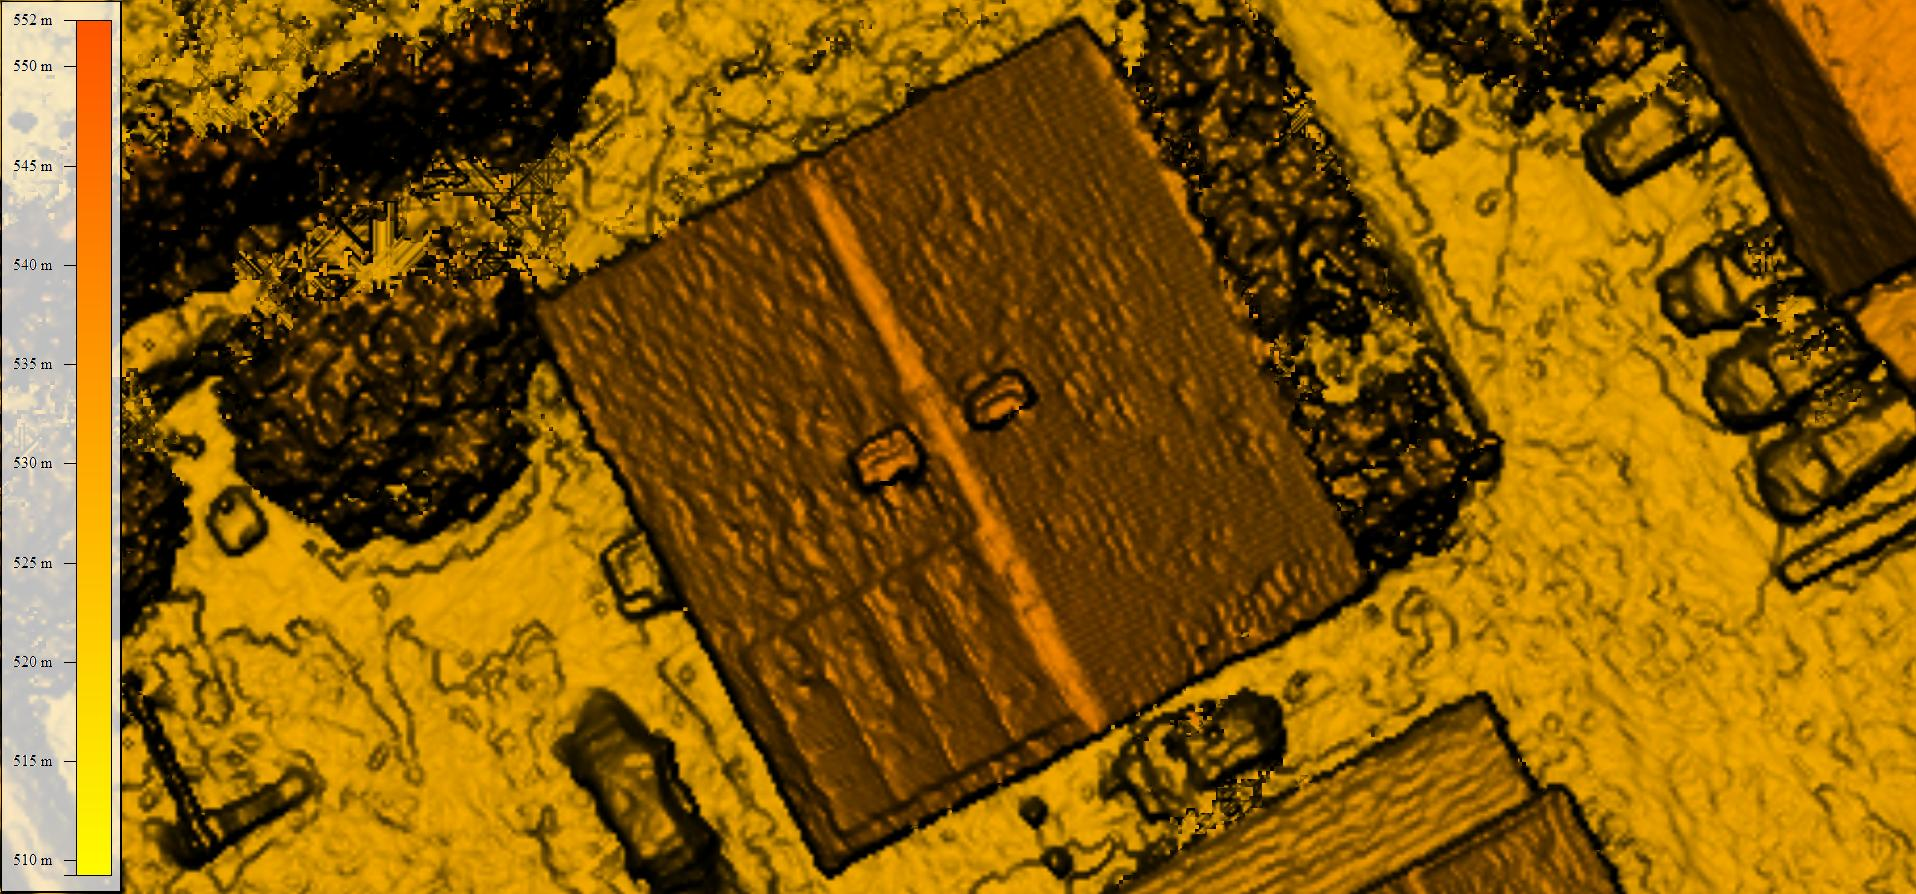
\includegraphics[width=\textwidth]{figs/Roof_DSM_NA+OBL_10cm.jpg}
		\subcaption{DSM with poor aerial triangulation}\label{fig:dim:c}
	\end{subfigure}
	\caption{Errors in aerial triangulation can lead to distortions in the DSM (derived from dense image matching). Images courtesy of Vermessung AVT.}%
\label{fig:dim}
\end{figure*}


\subsection{Target surface}
Many commonly occurring  artefacts  happen due to properties of the target surface. We distinguish three classes.

\subsubsection{Geometry} 
The shape of the target surfaces in relation to the sensor position has a great effect on 1) local point densities and 2) occlusion. As you can see from Figure~\ref{fig:lidarAcquisitionConditions:a},
\begin{marginfigure}
	\centering
	\includegraphics[width=\textwidth,page=2]{figs/lidarAcq.pdf}
	\caption{Point distribution and occlusion}%
	\label{fig:lidarAcquisitionConditions:a}
\end{marginfigure}
which illustrates this for lidar, surfaces that are closest to the scanner and orthogonal to the laser beams will yield the highest point densities (see the rooftop of the middle house). Very steep surfaces on the other hand, yield relatively low point densities (see the façades of the buildings). 

\emph{Occlusion} happens when a surface is not visible from the scanner position.% 
\index{occlusion}
As a result there will be gaps in the point coverage, also visible in Figure~\ref{fig:lidarAcquisitionConditions:a}. 
Notice how some steep surfaces and some of the adjacent ground are not registered at all by the scanner because it simply could not `see' these parts.

The severity of both effects mostly depends on the geometry of the target objects and flight parameters such as the flying altitude and the amount of overlap between flight strips.
However, regardless of what flight parameters are chosen for a survey both effects are almost always visible somewhere in the resulting dataset, see for example Figure~\ref{fig:pcd} for different lidar datasets for the same area.

% oblique vs nadir for occlusion
%Especially occlusion can be a problem for (2.5D) DTM generation because it causes no-data areas that may be problematic.

\begin{figure*}
	\centering
	\begin{subfigure}{0.45\linewidth}
		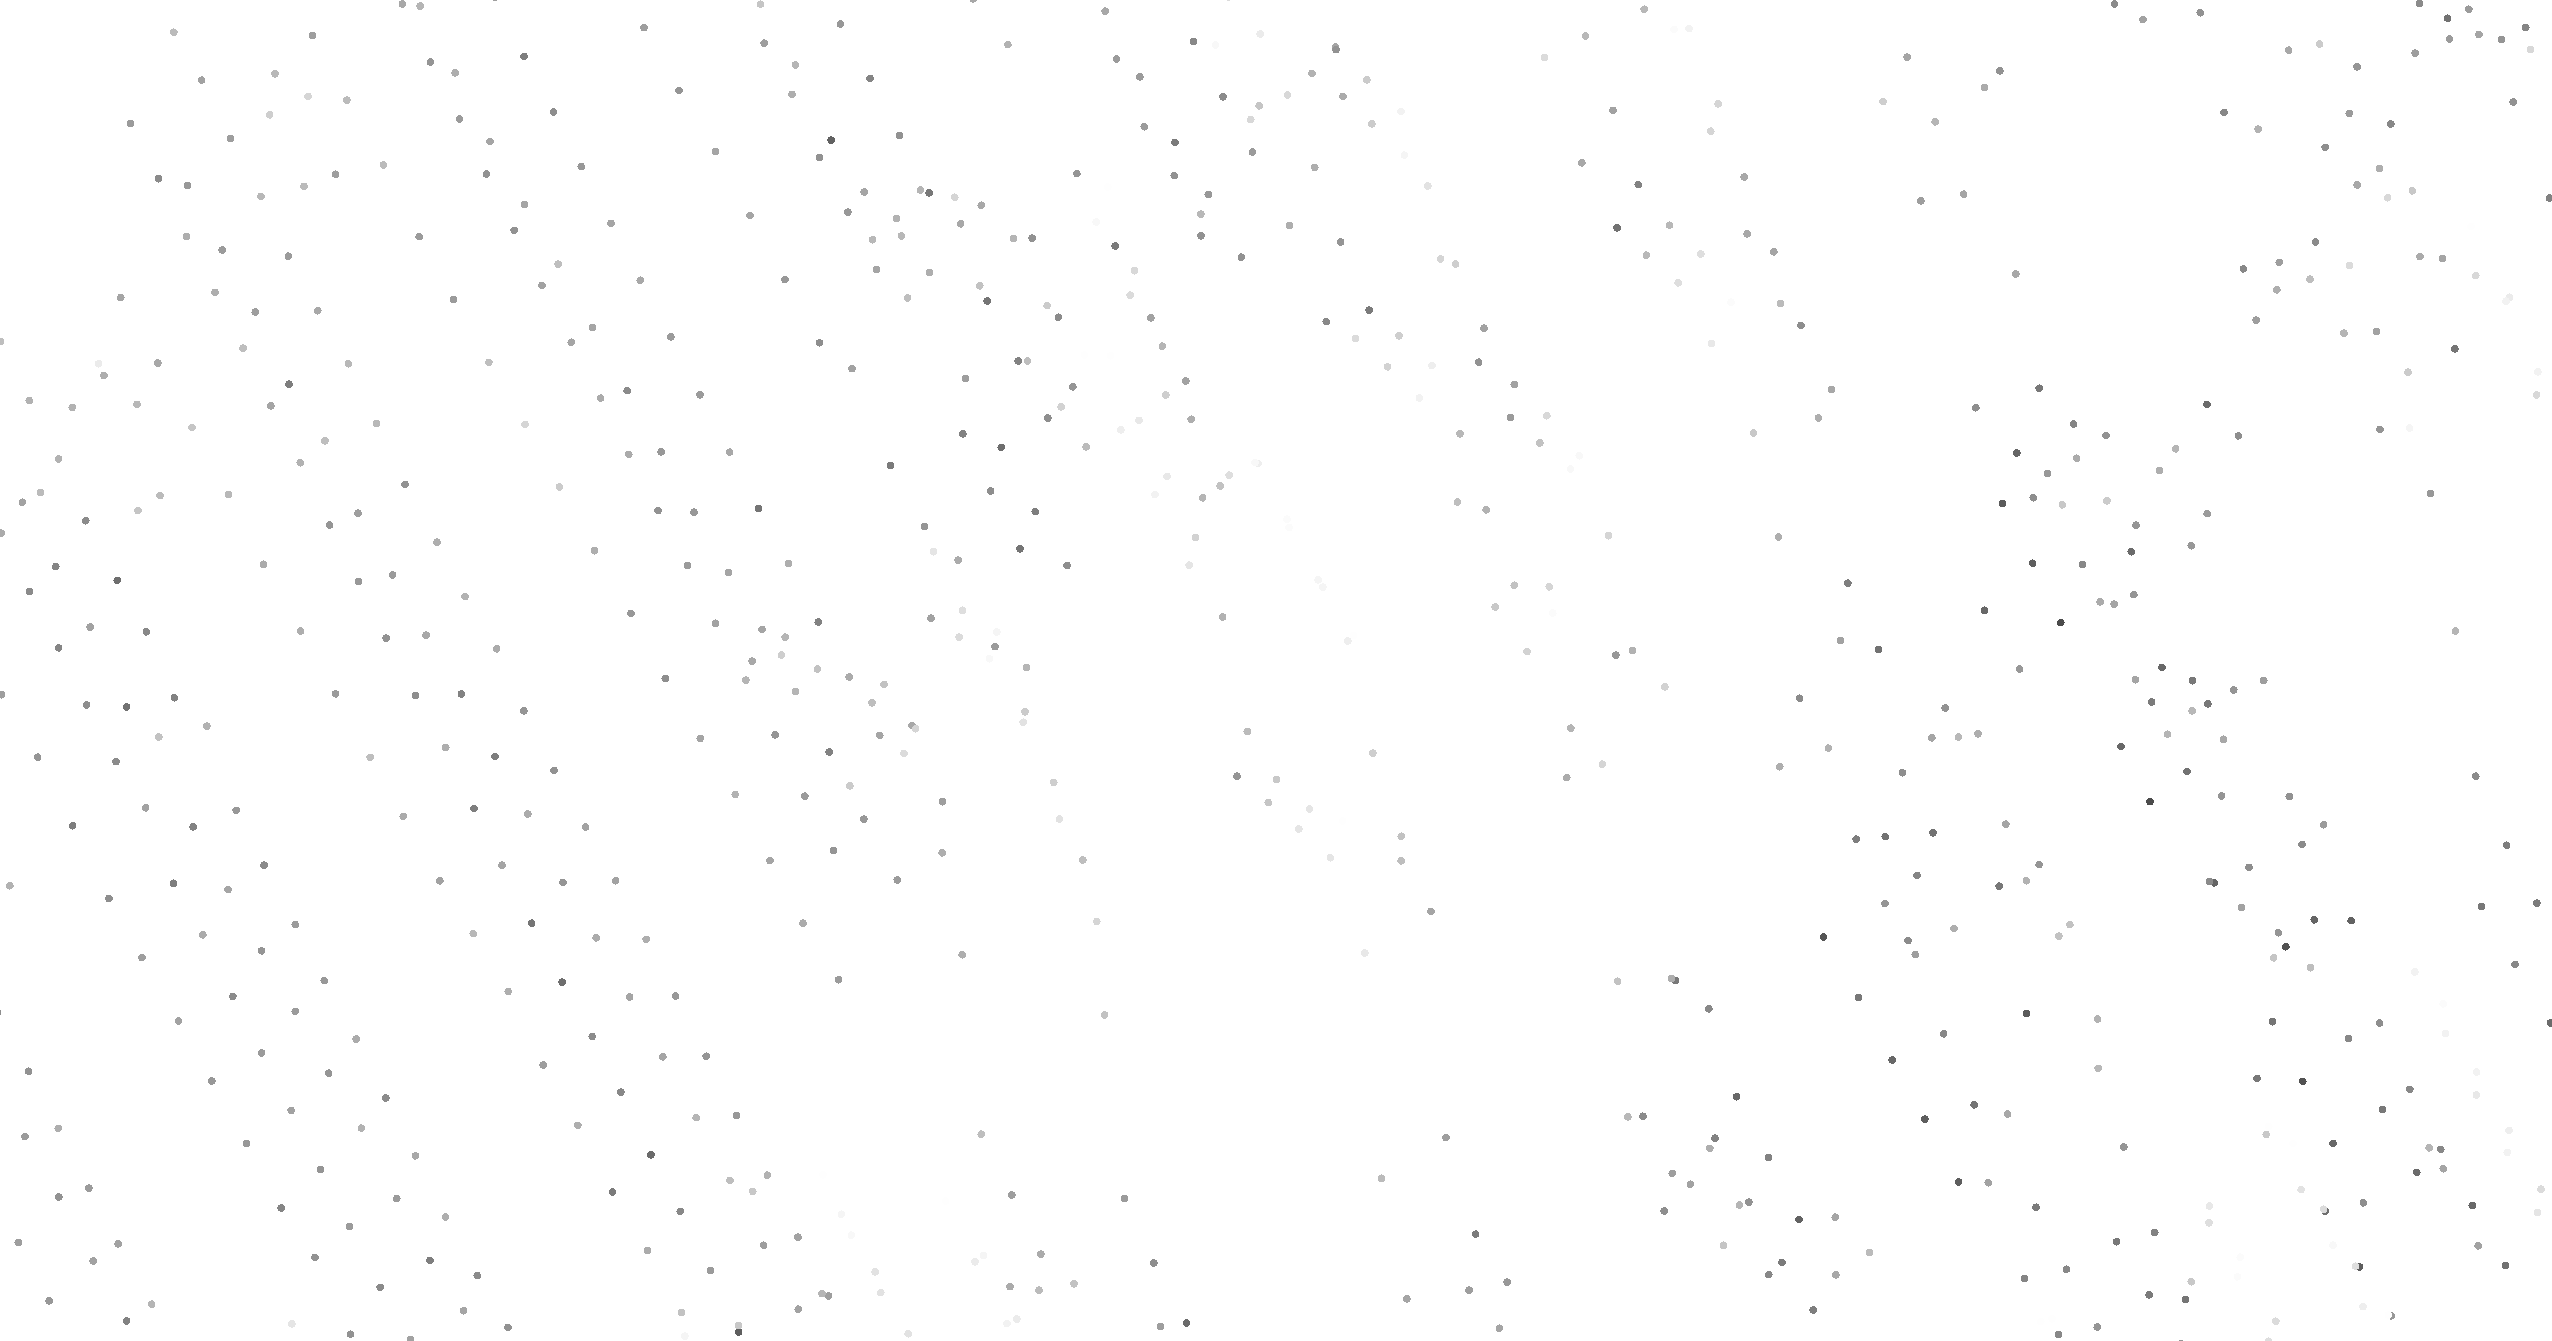
\includegraphics[width=\textwidth]{figs/ahn1_d.png}
		\subcaption{AHN1 (1996--2003)}\label{fig:pcd:ahn1}
	\end{subfigure}
	\quad
	\begin{subfigure}{0.45\linewidth}
		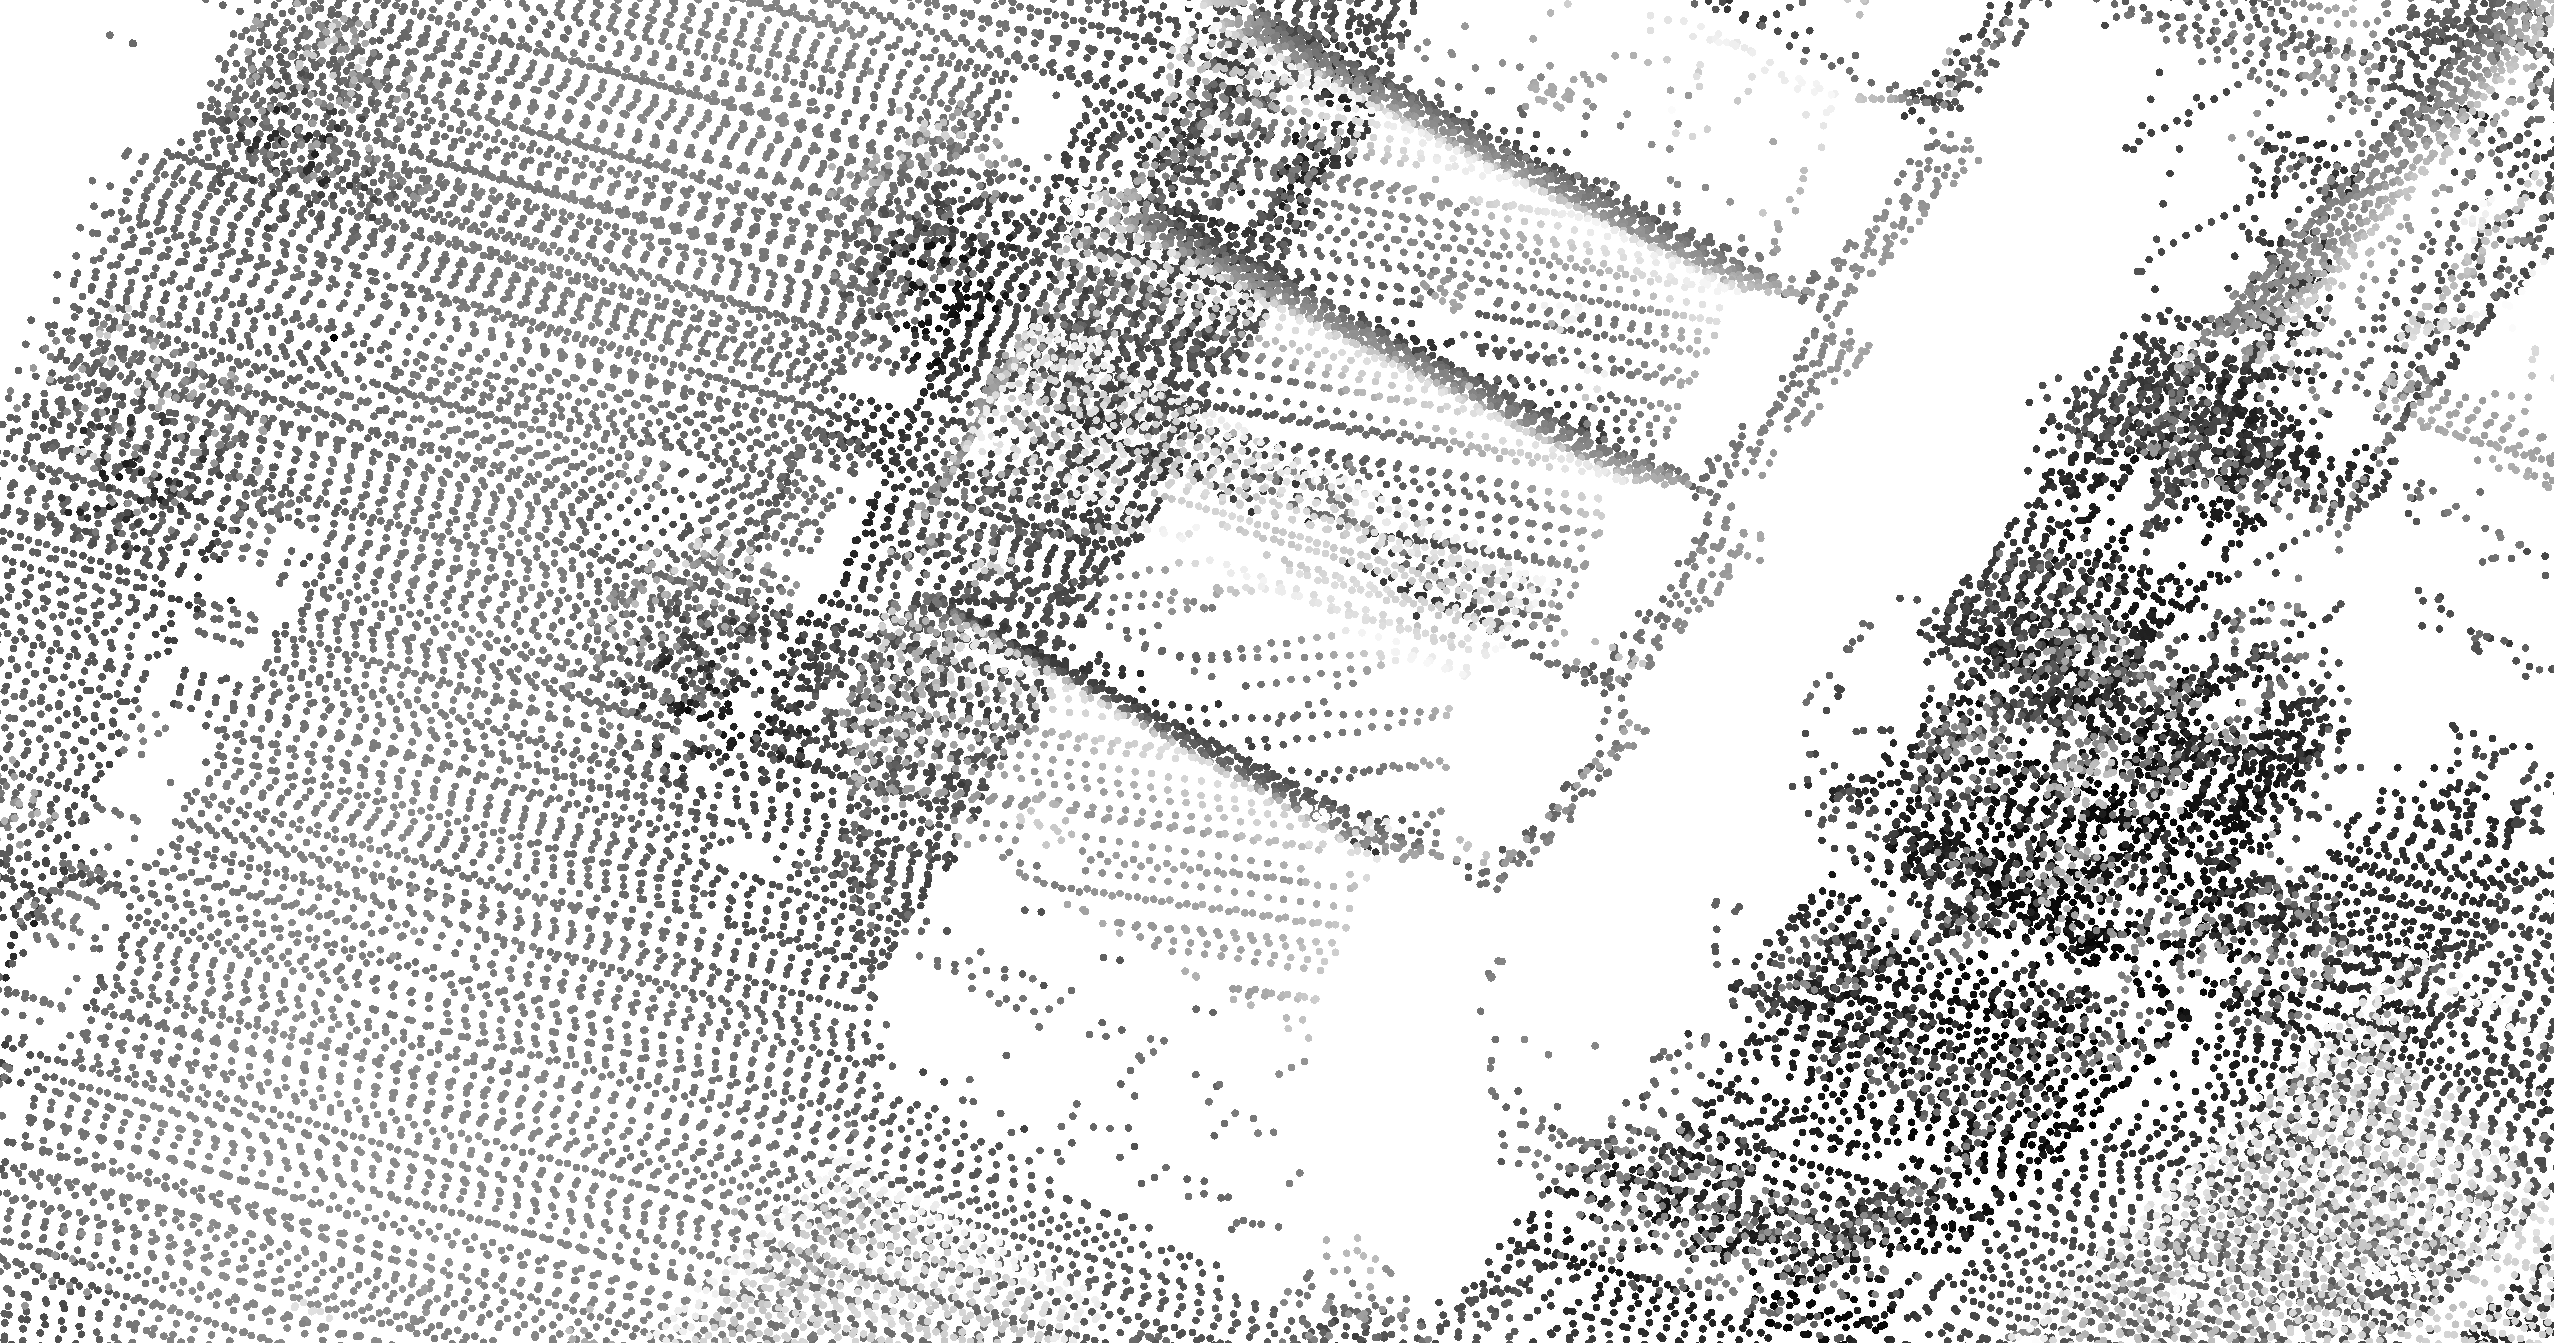
\includegraphics[width=\textwidth]{figs/ahn2_d.png}
		\subcaption{AHN2 (2008)}\label{fig:pcd:ahn2}
	\end{subfigure}
	
	\begin{subfigure}{0.45\linewidth}
		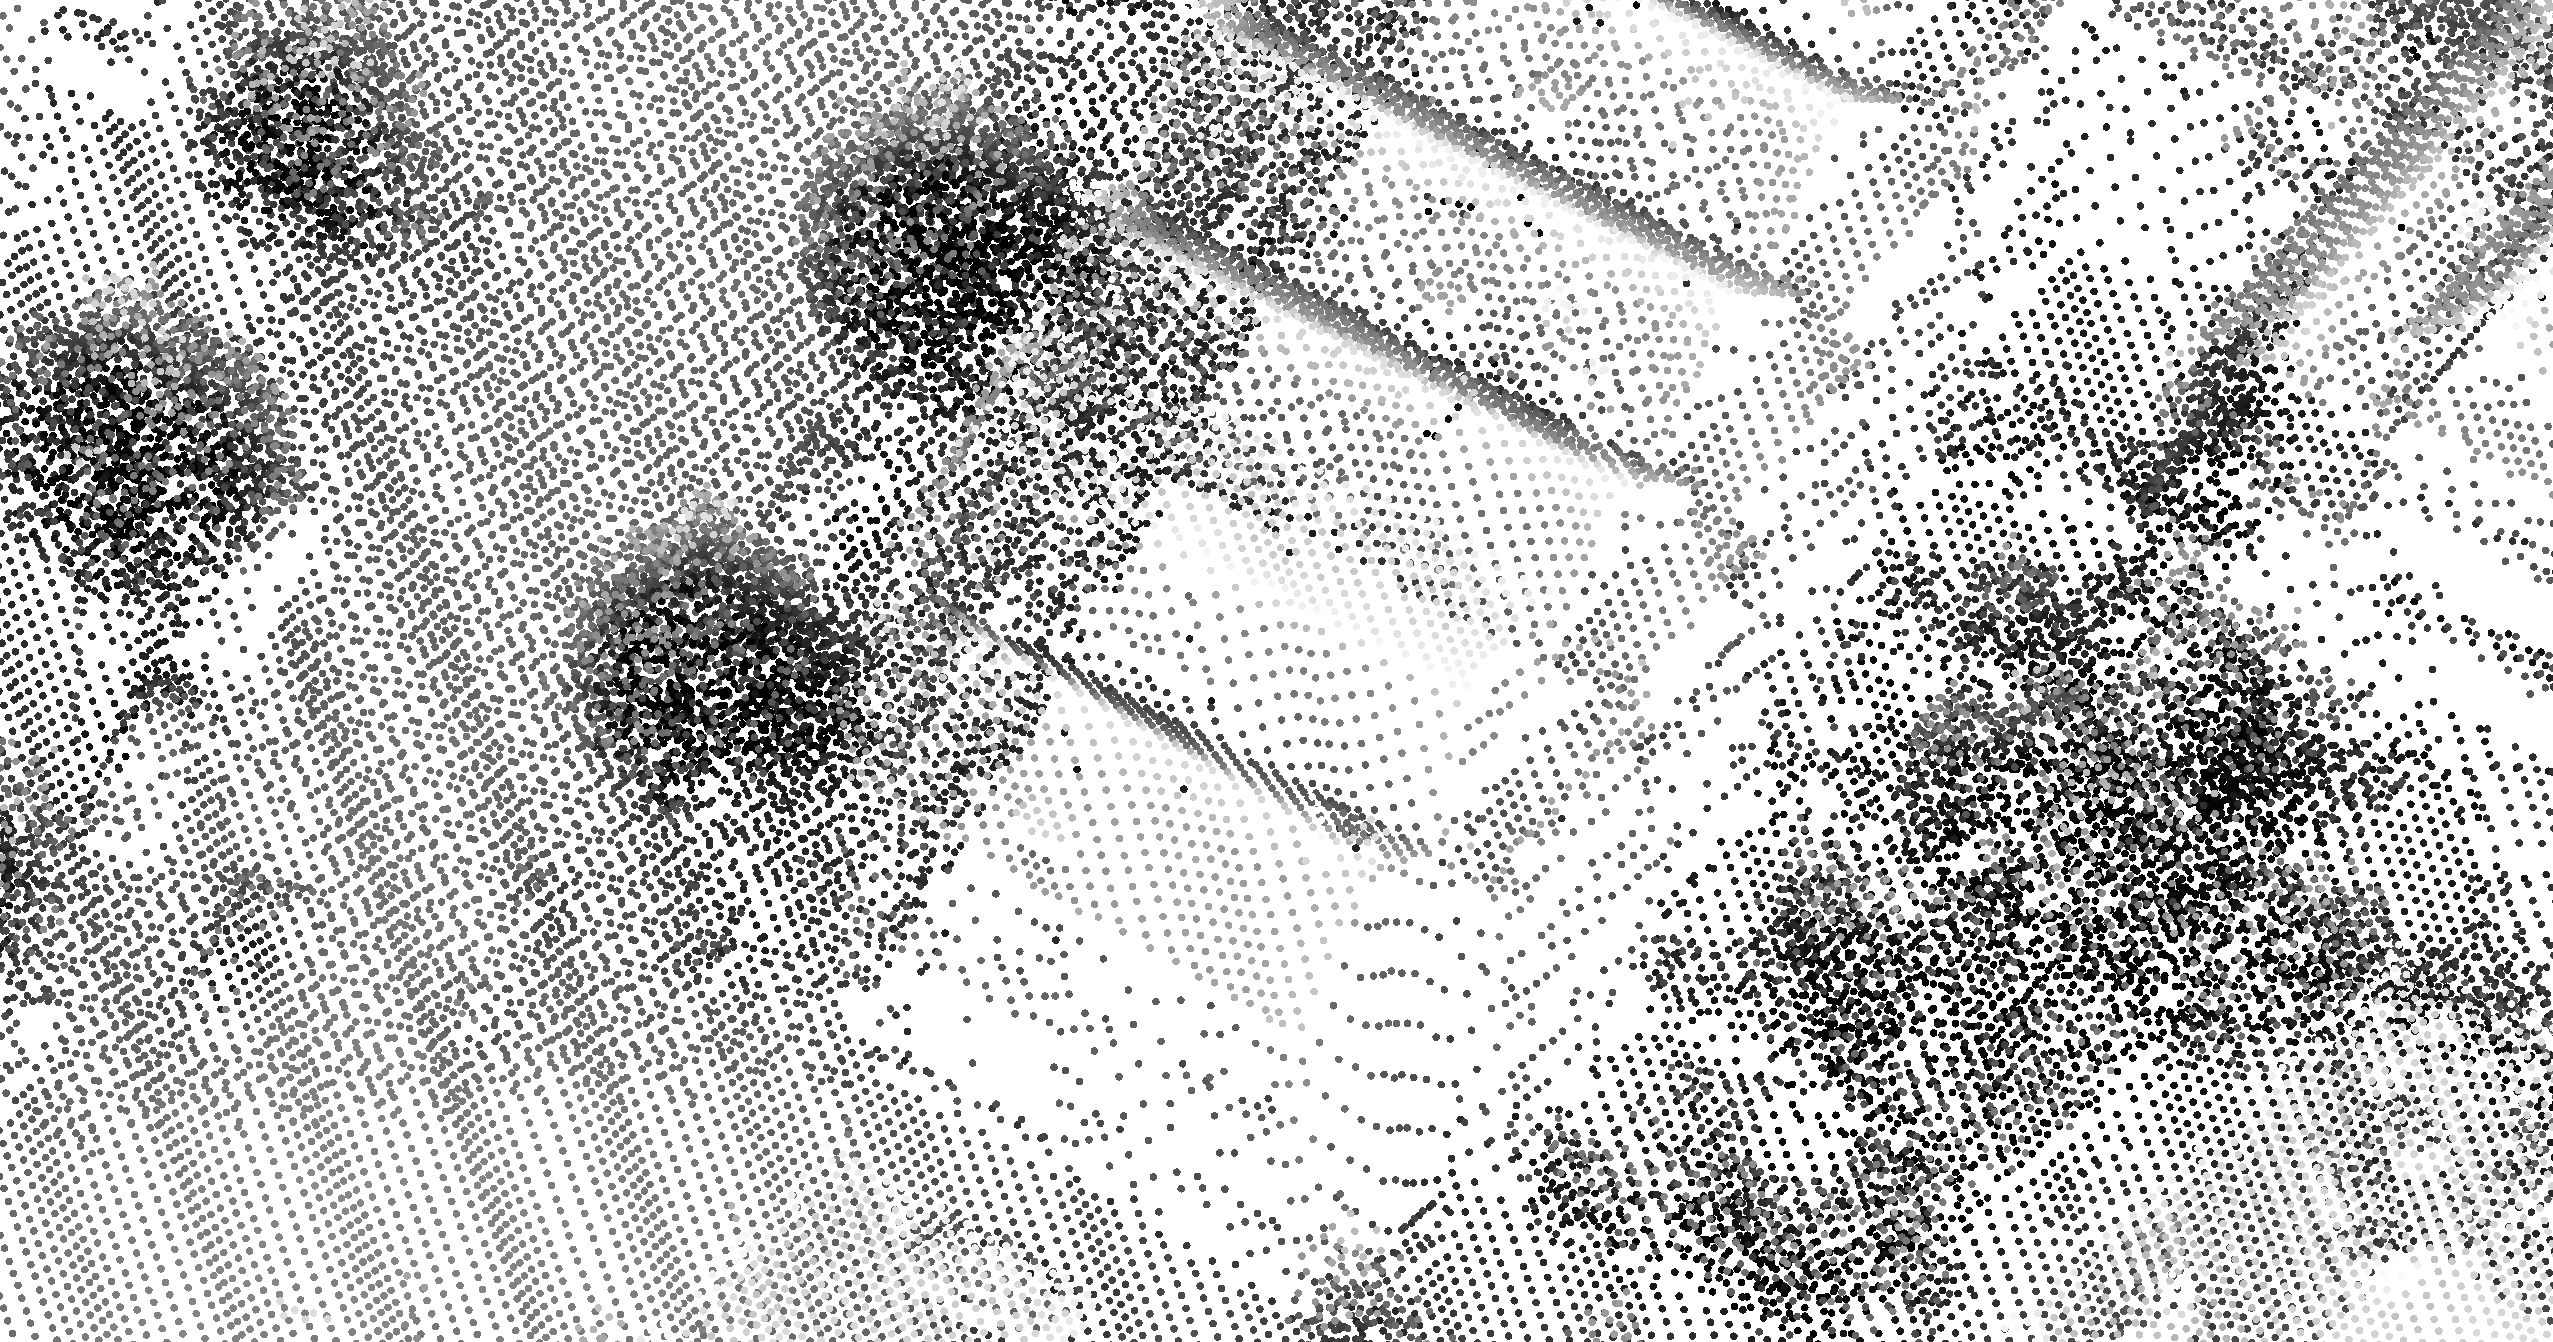
\includegraphics[width=\textwidth]{figs/ahn3_d.png}
		\subcaption{AHN3 (2014)}\label{fig:pcd:ahn3}
	\end{subfigure}
	\quad
	\begin{subfigure}{0.45\linewidth}
		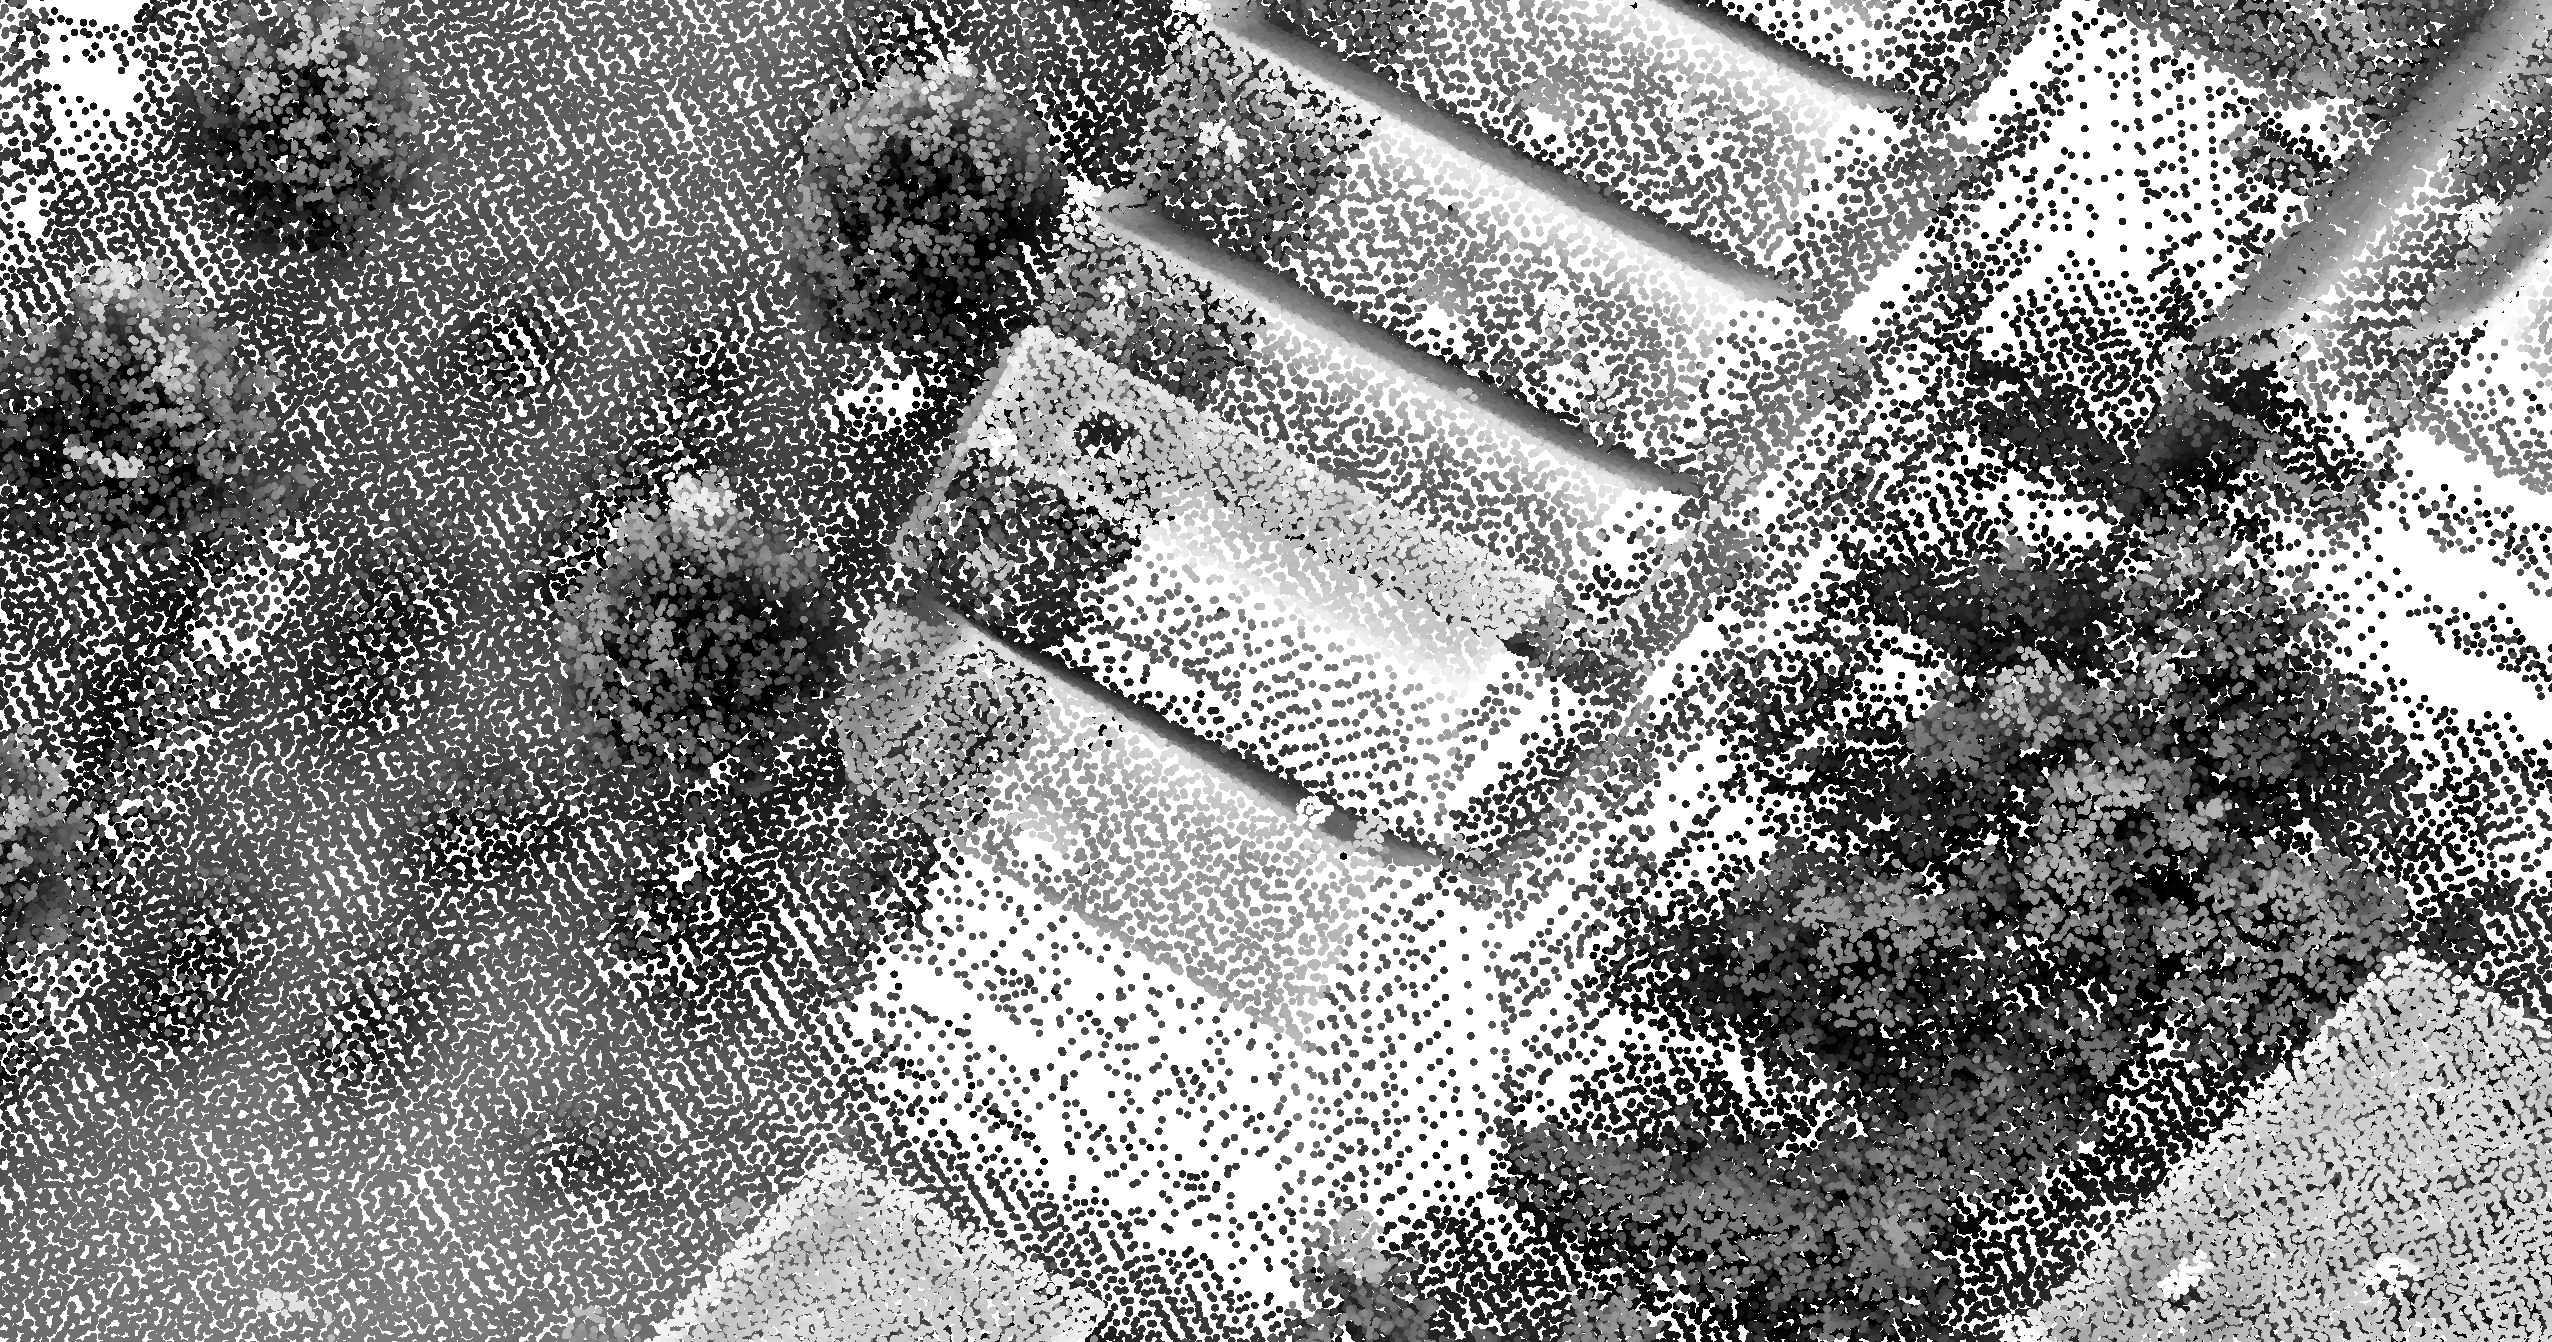
\includegraphics[width=\textwidth]{figs/rdam16_d.png}
		\subcaption{City of Rotterdam (2016)}\label{fig:pcd:rdam16}
	\end{subfigure}
	\caption{Several lidar point clouds for the same area in the city of Rotterdam. Point distribution and occlusion effects vary.}%
\label{fig:pcd}
\end{figure*}

\subsubsection{Material properties}
Depending on material properties of a target surface, signals may be reflected in a way that makes it impossible to compute the correct distance. 
Surfaces that act like a mirror are especially problematic, Figure~\ref{fig:lidarAcquisitionConditions:b} illustrates this. 
\begin{marginfigure}
	\centering
	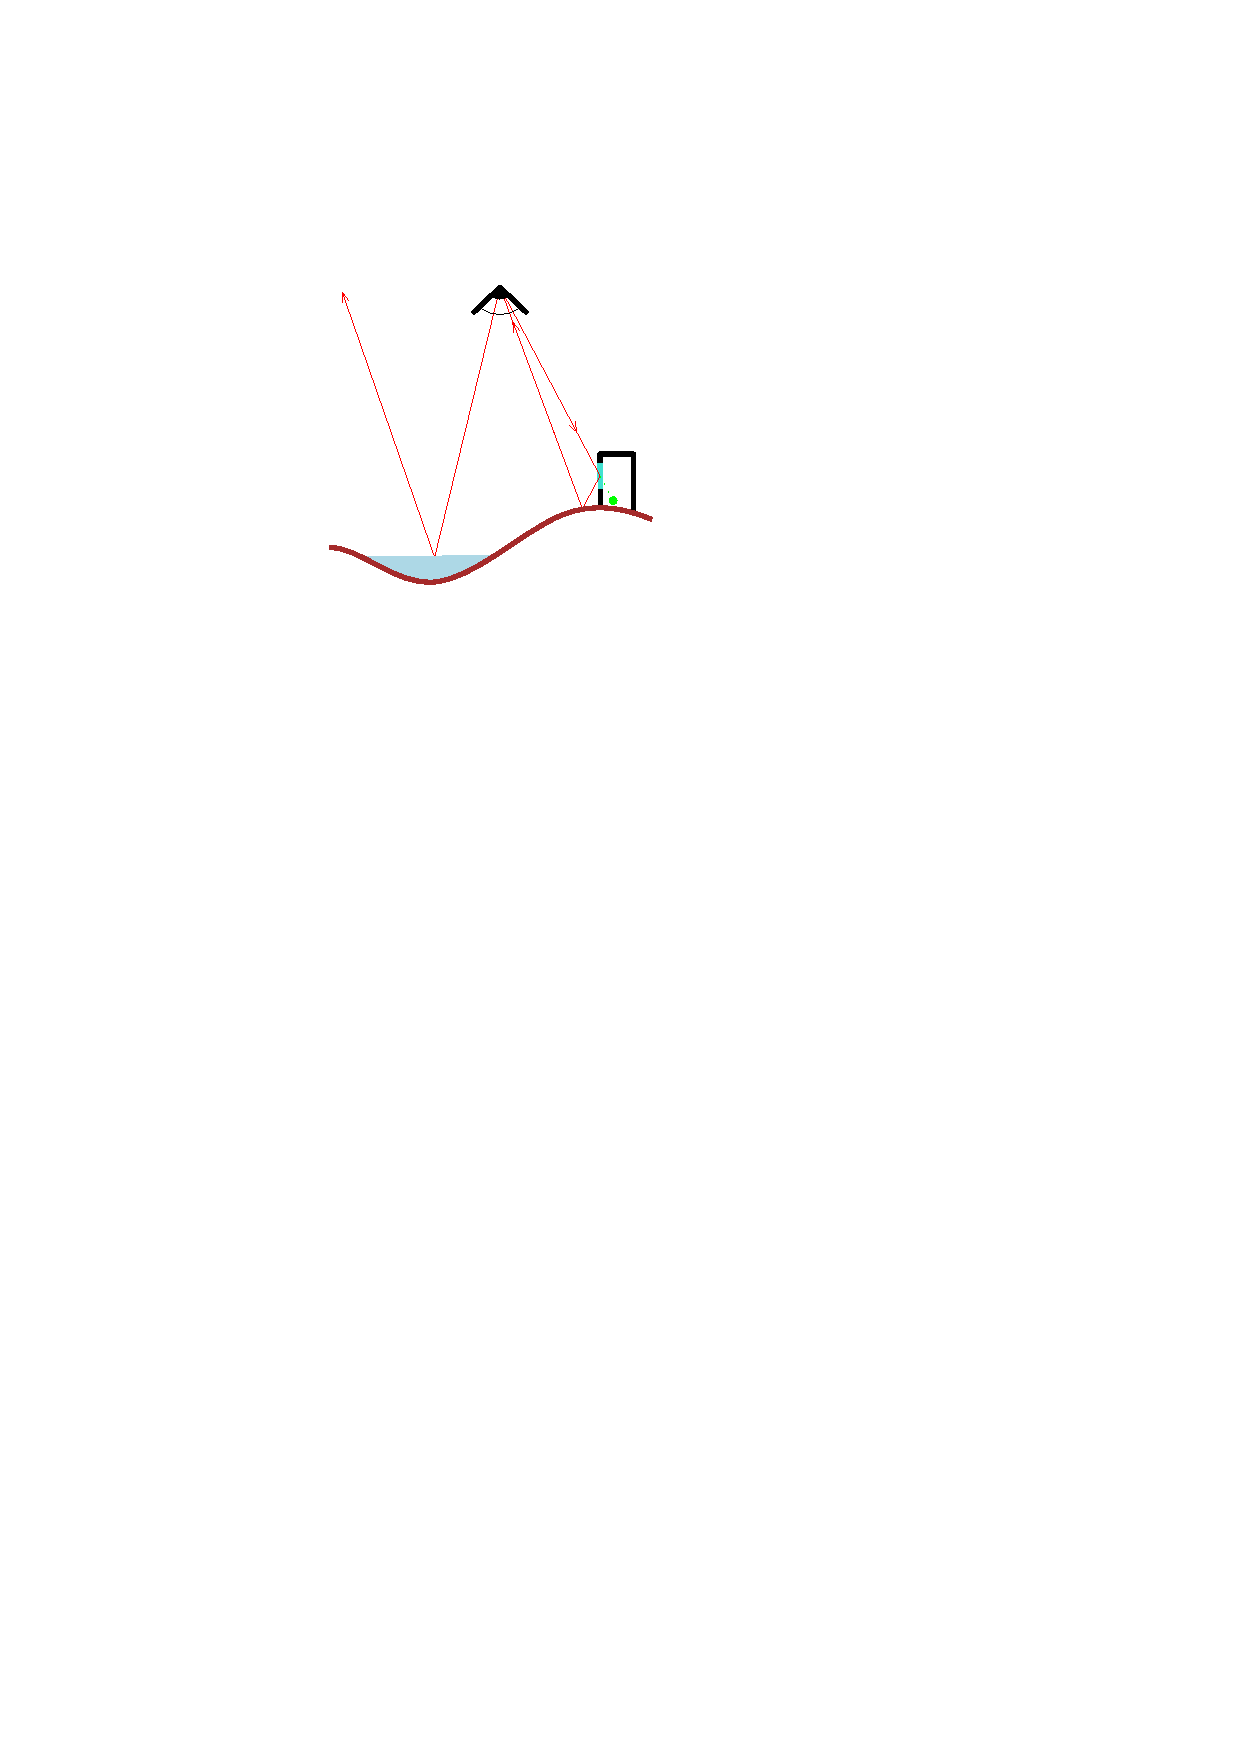
\includegraphics[width=\textwidth,page=1]{figs/lidarAcq.pdf}
	\caption{Reflection and multi-path}%
	\label{fig:lidarAcquisitionConditions:b}
\end{marginfigure}
First, it may happen that a pulse is reflected away from the sensor, \eg\ from a water surface, resulting in no distance measurement for that pulse. 
Or, in the case of photogrammetry, we will observe a different reflection in each image which heavily distorts the matching process, sometimes resulting in extreme outliers for water surfaces.  
In some cases, and only for active sensors, the reflected pulse does make its way back to the sensor, see for example the right half of Figure~\ref{fig:lidarAcquisitionConditions:b}. 
However, it will have travelled a longer distance than it should have and the scanner only knows in which direction it emitted the pulse. 
This effect is called \emph{multi-path} and the result is that points are measured at a distance that is too long and therefore they show up below the ground surface in the point cloud (see Figure~\ref{fig:outliers}).  
\begin{figure}
	\centering
	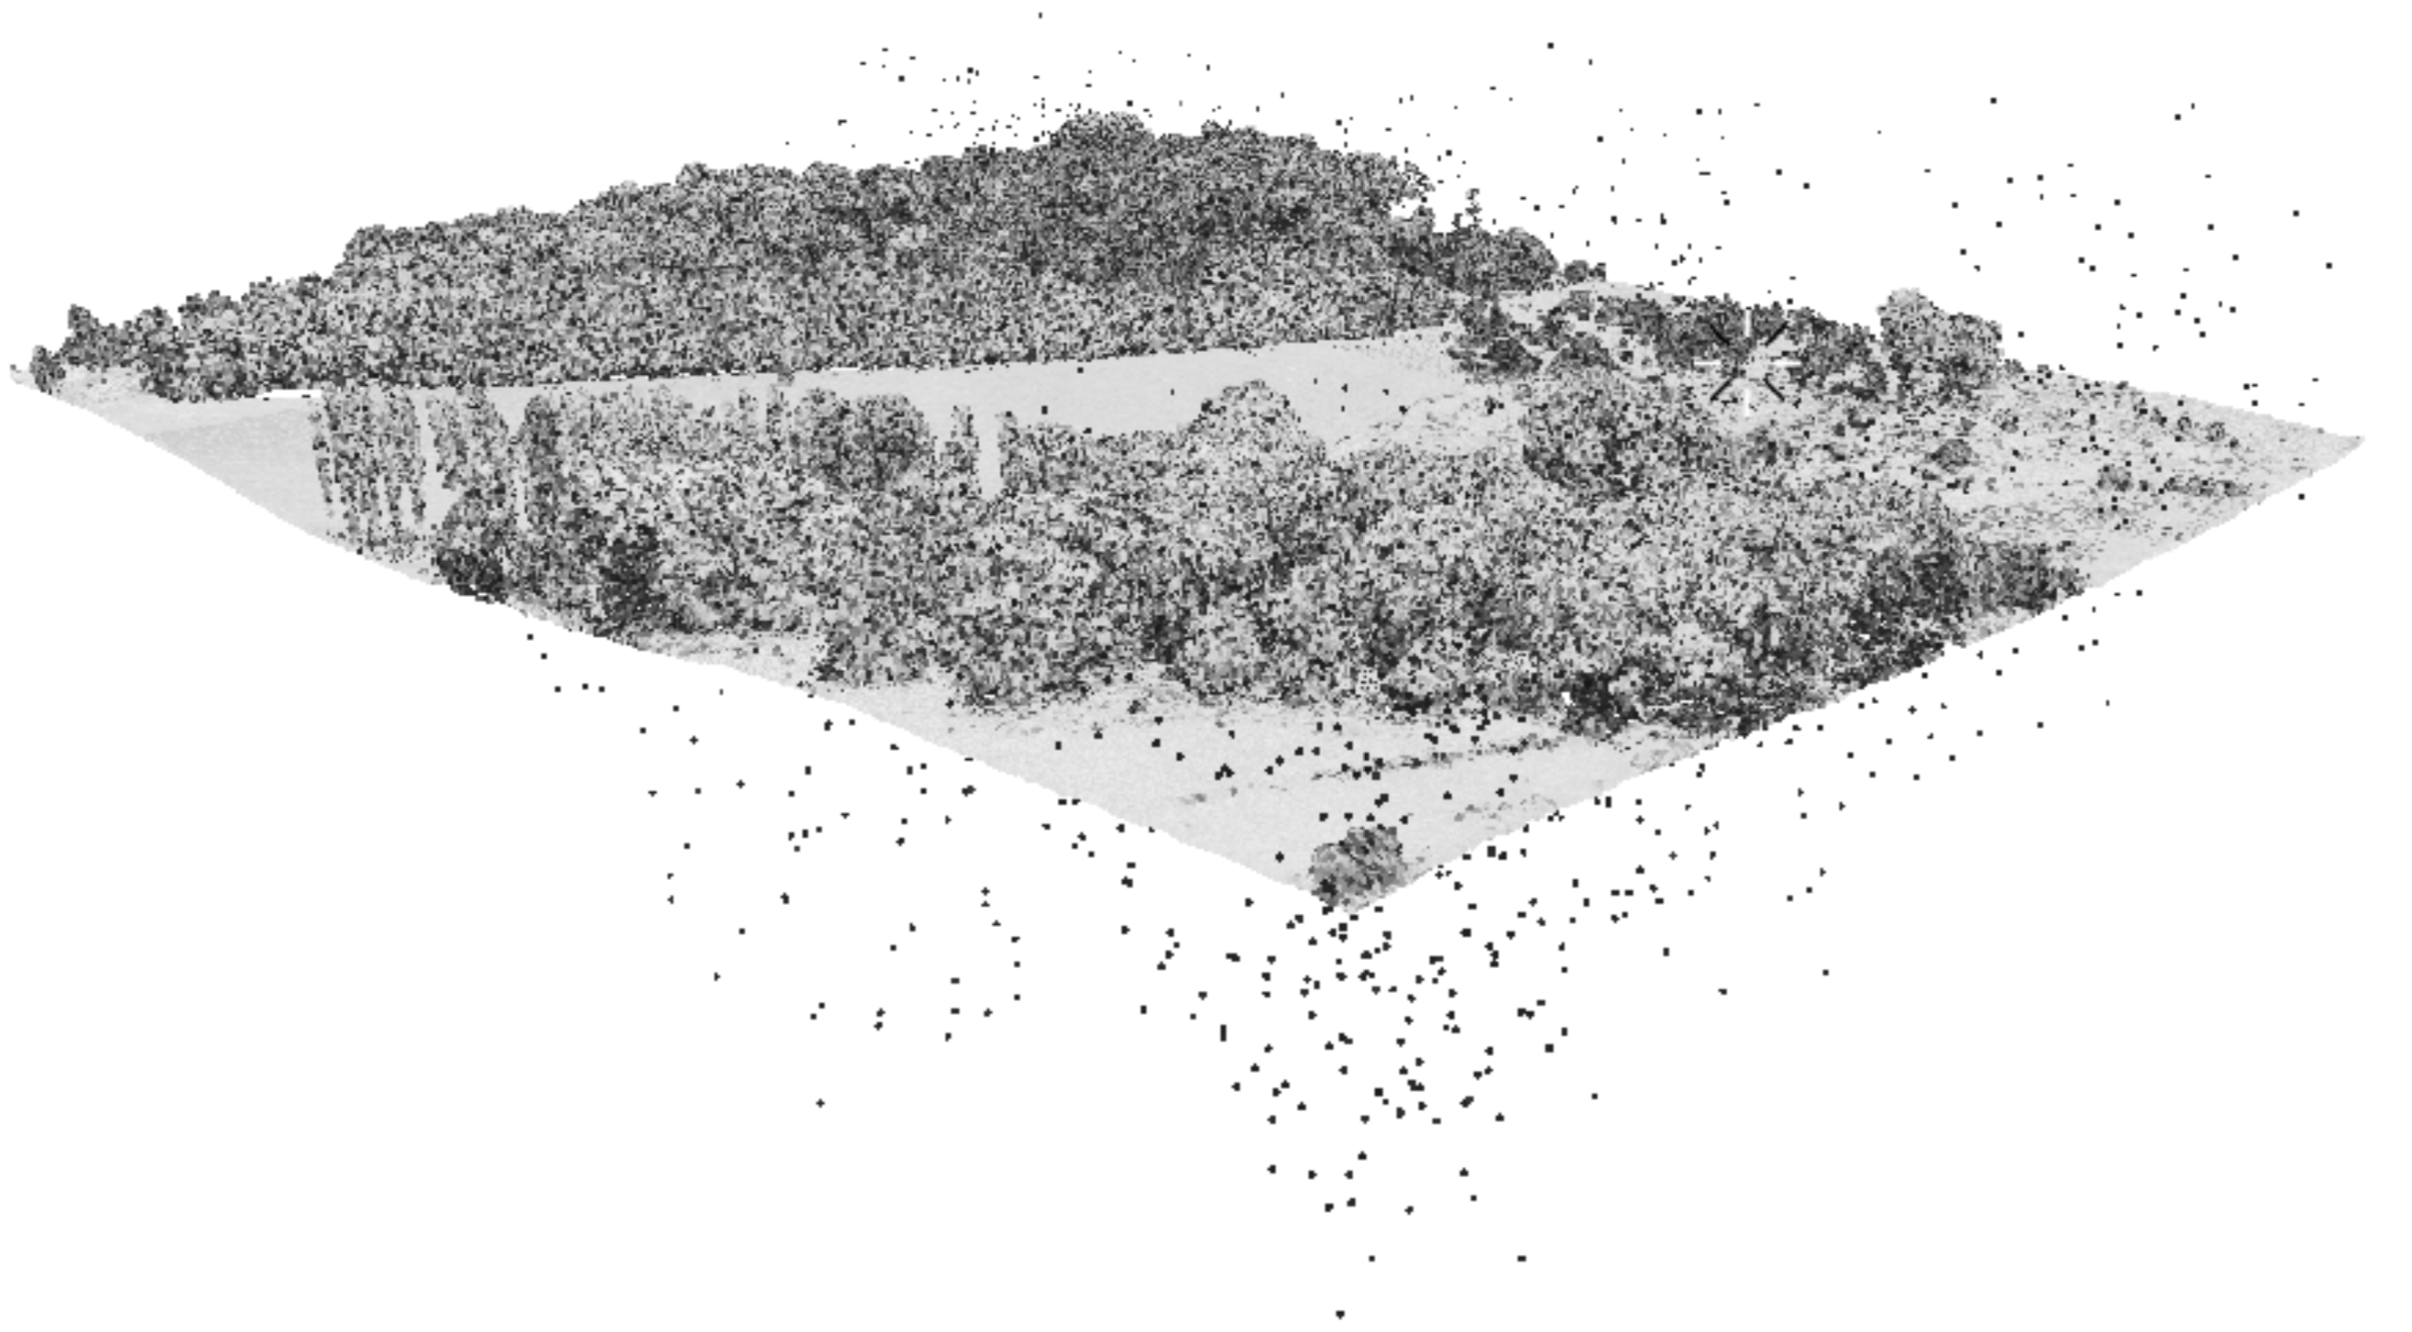
\includegraphics[width=\textwidth]{figs/outliers.png}
	\caption{Outliers, below and above the ground, in a lidar point cloud dataset.}%
\label{fig:outliers}
\end{figure}

Photogrammetry suffers from a few other problems as well, such as surfaces that have a homogeneous texture that make it impossible to find distinguishing features that can be used for matching. 
This may also happen in poor lightning conditions, for example in the shadow parts of an image.
%no texture (shadow), multi-path, complete absorption lightning conditions: shadow poor matching

\subsubsection{Moving objects}
An example of moving objects are flocks of birds flying in front of the scanner. These can cause outliers high above the ground, as illustrated in Figure~\ref{fig:outliers}.


\subsection{Processing}
It is common to perform some kind of process after acquisition in order to fix errors caused by the reasons mentioned above. 
In most cases such processes are largely successful. 
For instance, one can attempt to fill the void regions, sometimes referred to as \emph{no-data} regions, that are for instance due to pools of rainwater or occlusion, using an interpolation method (Figure~\ref{fig:voidfill}).
\begin{figure*}
	\centering
	\begin{subfigure}{0.45\linewidth}
		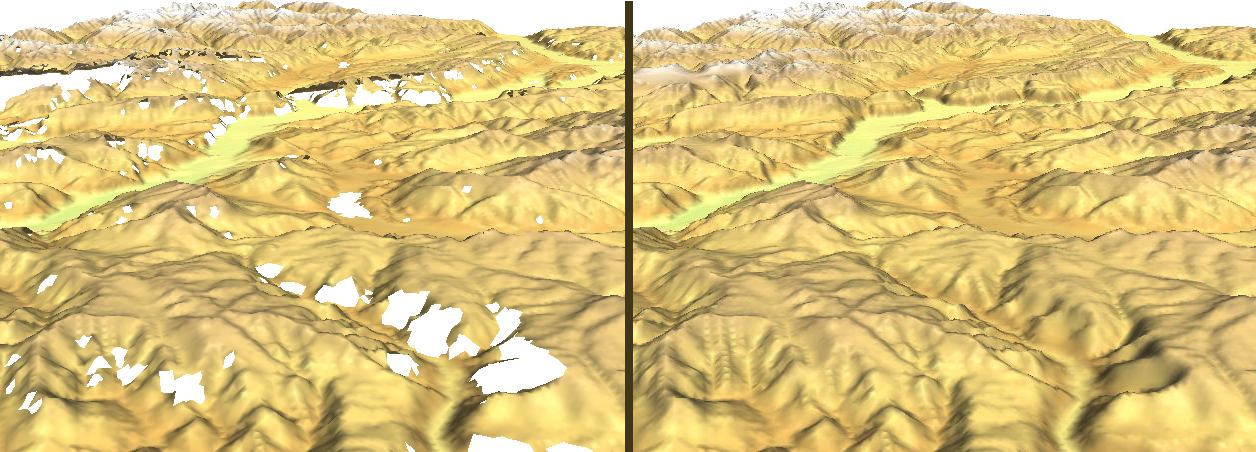
\includegraphics[width=\textwidth]{figs/srtm_trento_voidfill.png}
		\subcaption{Void-filling through interpolation in SRTM data}\label{fig:voidfill}
	\end{subfigure}
	\quad
	\begin{subfigure}{0.45\linewidth}
		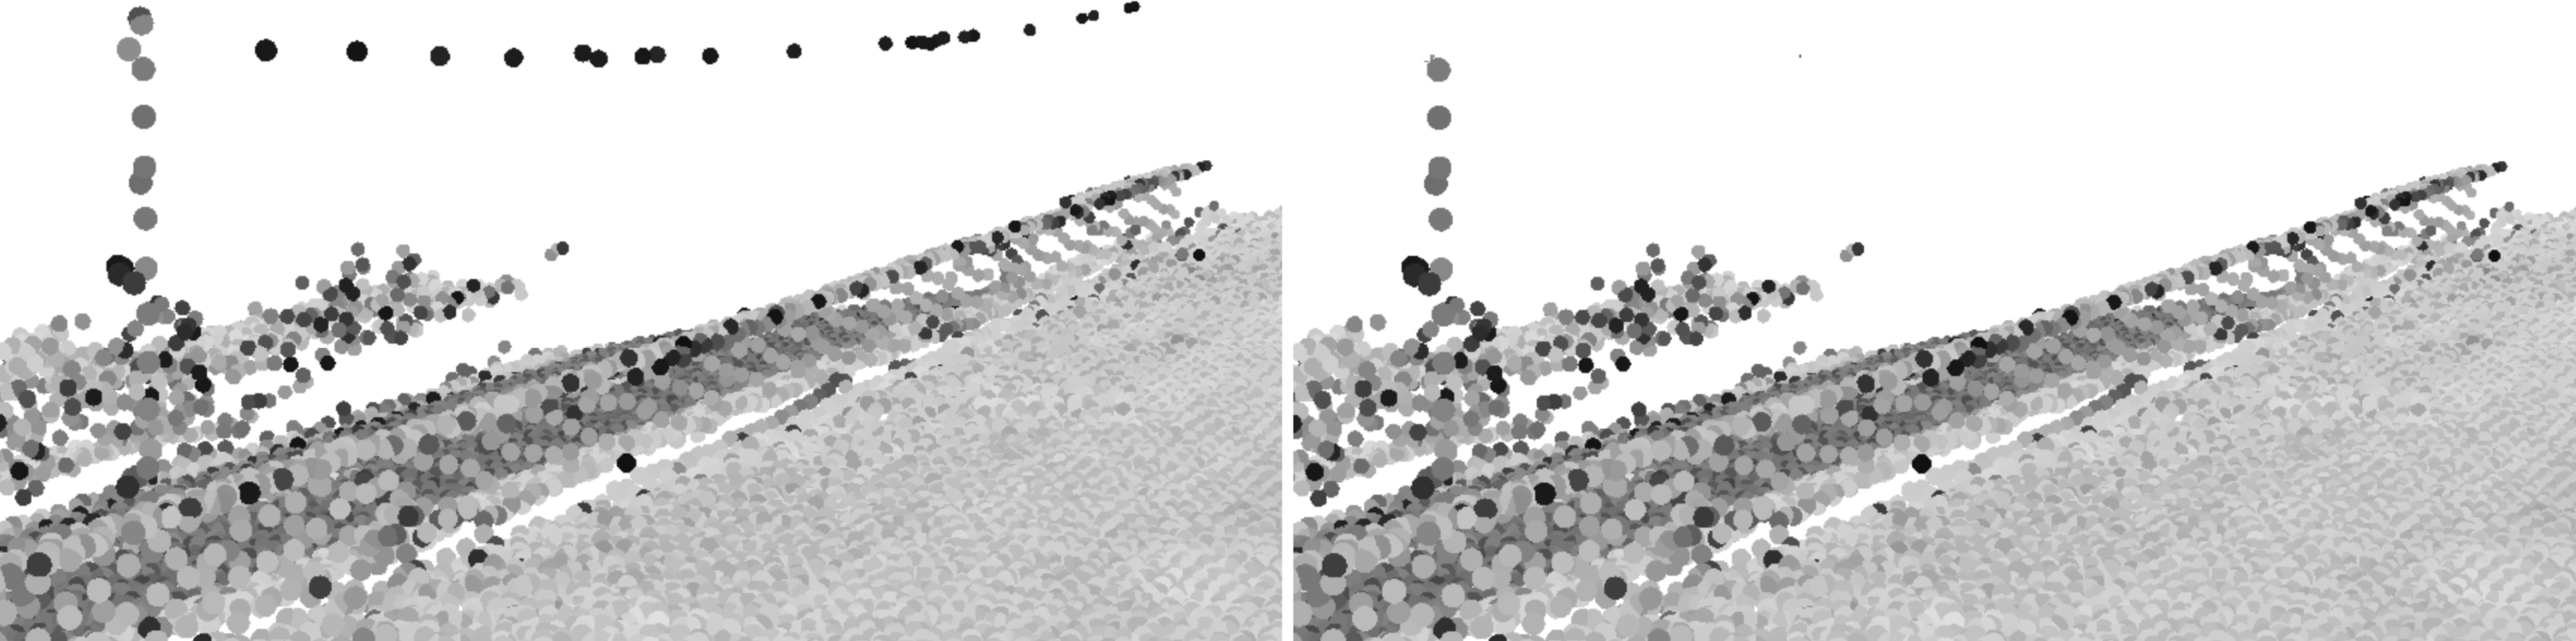
\includegraphics[width=\textwidth]{figs/ourlier-detection-wrong.png}
		\subcaption{Good points, \ie\ those on the power line, may be removed during outlier detection}\label{fig:outlier-wrong}
	\end{subfigure}
	\caption{Post-processing aimed at correcting artefacts. Before processing (left) and after processing (right).}%
	\label{fig:processing}
\end{figure*}
Or, one can attempt to detect and remove outliers caused \eg\ by multi-path effects or flocks of birds\sidenote{This is a topic of Chapter~\ref{chap:pcprocessing}}. 
However, while the intention is always to reduce the number and severity of artefacts, these processes sometimes introduce distortions of their own.
For example, an outlier detection algorithm may remove `good' points if they look the same as outliers to the outlier detection algorithm (see \eg\ Figure~\ref{fig:outlier-wrong}).
And void-filling is only effective if the void area is not too large, since interpolation methods always assume there is sufficient neighbourhood information to work with\sidenote{Chapters~\ref{chap:interpol} and~\ref{chap:kriging} explore the topic of spatial interpolation in detail.}.


%%
\begin{kaobox-toread}[frametitle=\faExternalLink\ To read or to watch]
This is a paper that compares lidar and photogrammetry derived point clouds for the generation of a DEM\@. It shows that even when artefacts seem to be under control, both techniques may measure different elevations 

\fullcite{Ressl16}
\textbf{PDF:} \url{https://3d.bk.tudelft.nl/courses/geo1015/data/others/Ressl16.pdf}
\end{kaobox-toread}

%For instance, an outlier filter 
%misclassified points, smoothing effects in DIM

% Difficulties in automated DTM generation
% - Homogeneous areas and repeating structures;
% - No distinct peak or multiple peaks of the similarity measures
% - Areas occluded in one image
% - No correspondence exists;
% - Steep sloped surfaces
% - Geometric difference between template and match window;
% - Discontinuities and break-lines
% - No correspondence or geometric difference;
% - Non-lambertian surfaces
% - Radiometric difference between template and match window;
% - Moving objects
% - correct correspondence, incorrect elevation

% strip misalignment
% occlusion/geometry of target surface vs scanning position, density of points
% season- leaves on trees
% lightning conditions/shadow for photogrammetry
% surface material - reflactance, absorbance, multi echo, multiple returns


%few words about sensor fusion?


%%%
%
\section{Notes and comments}
If you would like to learn more about how a lidar scanner works, the chapter from \citet{Chazette16} is recommended.
More details on InSAR can be found in the manual from \citet{ESA07}.

\citet{Reuter09} give an elaborate overview of the processing that needs to be done to derive a high quality (raster) DTM from raw elevation measurements.

% fixing dem artefacts: https://www.sciencedirect.com/science/article/pii/S0166248108000044

%%%%%%%%%%%%%%%%%%%%
%
\section{Exercises}

\begin{enumerate}
	\item Name three differences between point cloud acquisition with lidar and with photogrammetry.
	\item Explain what the time-of-flight principle entails.
	\item How can you minimise occlusion effects in a point cloud during acquisition?
	\item Why does positioning, using for instance GPS, play such an important role in acquisition?
\end{enumerate}
     %- 02
%!TEX root = ../terrainbook.tex
% chktex-file 46

\setchapterpreamble[u]{\margintoc}
\graphicspath{{gdem/figs/}}


\chapter{Global digital elevation models}% or global terrains
\label{chap:gdem}

We define as ``global digital elevation models'' (or global terrains; we refer to them as ``gDEMs'' in this book) the datasets that cover (most of) the Earth.%
\index{global DEM}
Those datasets require different acquisition methods from local datasets, since flying an airplane or performing local surveys at the scale of the Earth has not been done yet, and it would be prohibitively expensive.
The acquisition instruments for a global coverage must be \emph{space-borne}, \ie\ mounted on a satellite for instance.
Notice that the orbit of some satellites makes them technically non-global, but that we still refer to their datasets as global since they have a wide coverage, just restricted to certain latitudes.

%

It cannot be understated that before the introduction of gDEMs (with SRTM v1 in 2000, see below for more information), we had no way of knowing the elevation for a given location on the Earth.
Indeed, looking at the datasets listed and/or hosted at
\marginnote{\url{https://opentopography.org}}
OpenTopography (Figure~\ref{fig:dem_coverage}), we can observe that, even in 2022, local elevation datasets are mostly limited to developed countries.
\begin{figure}
  \centering
  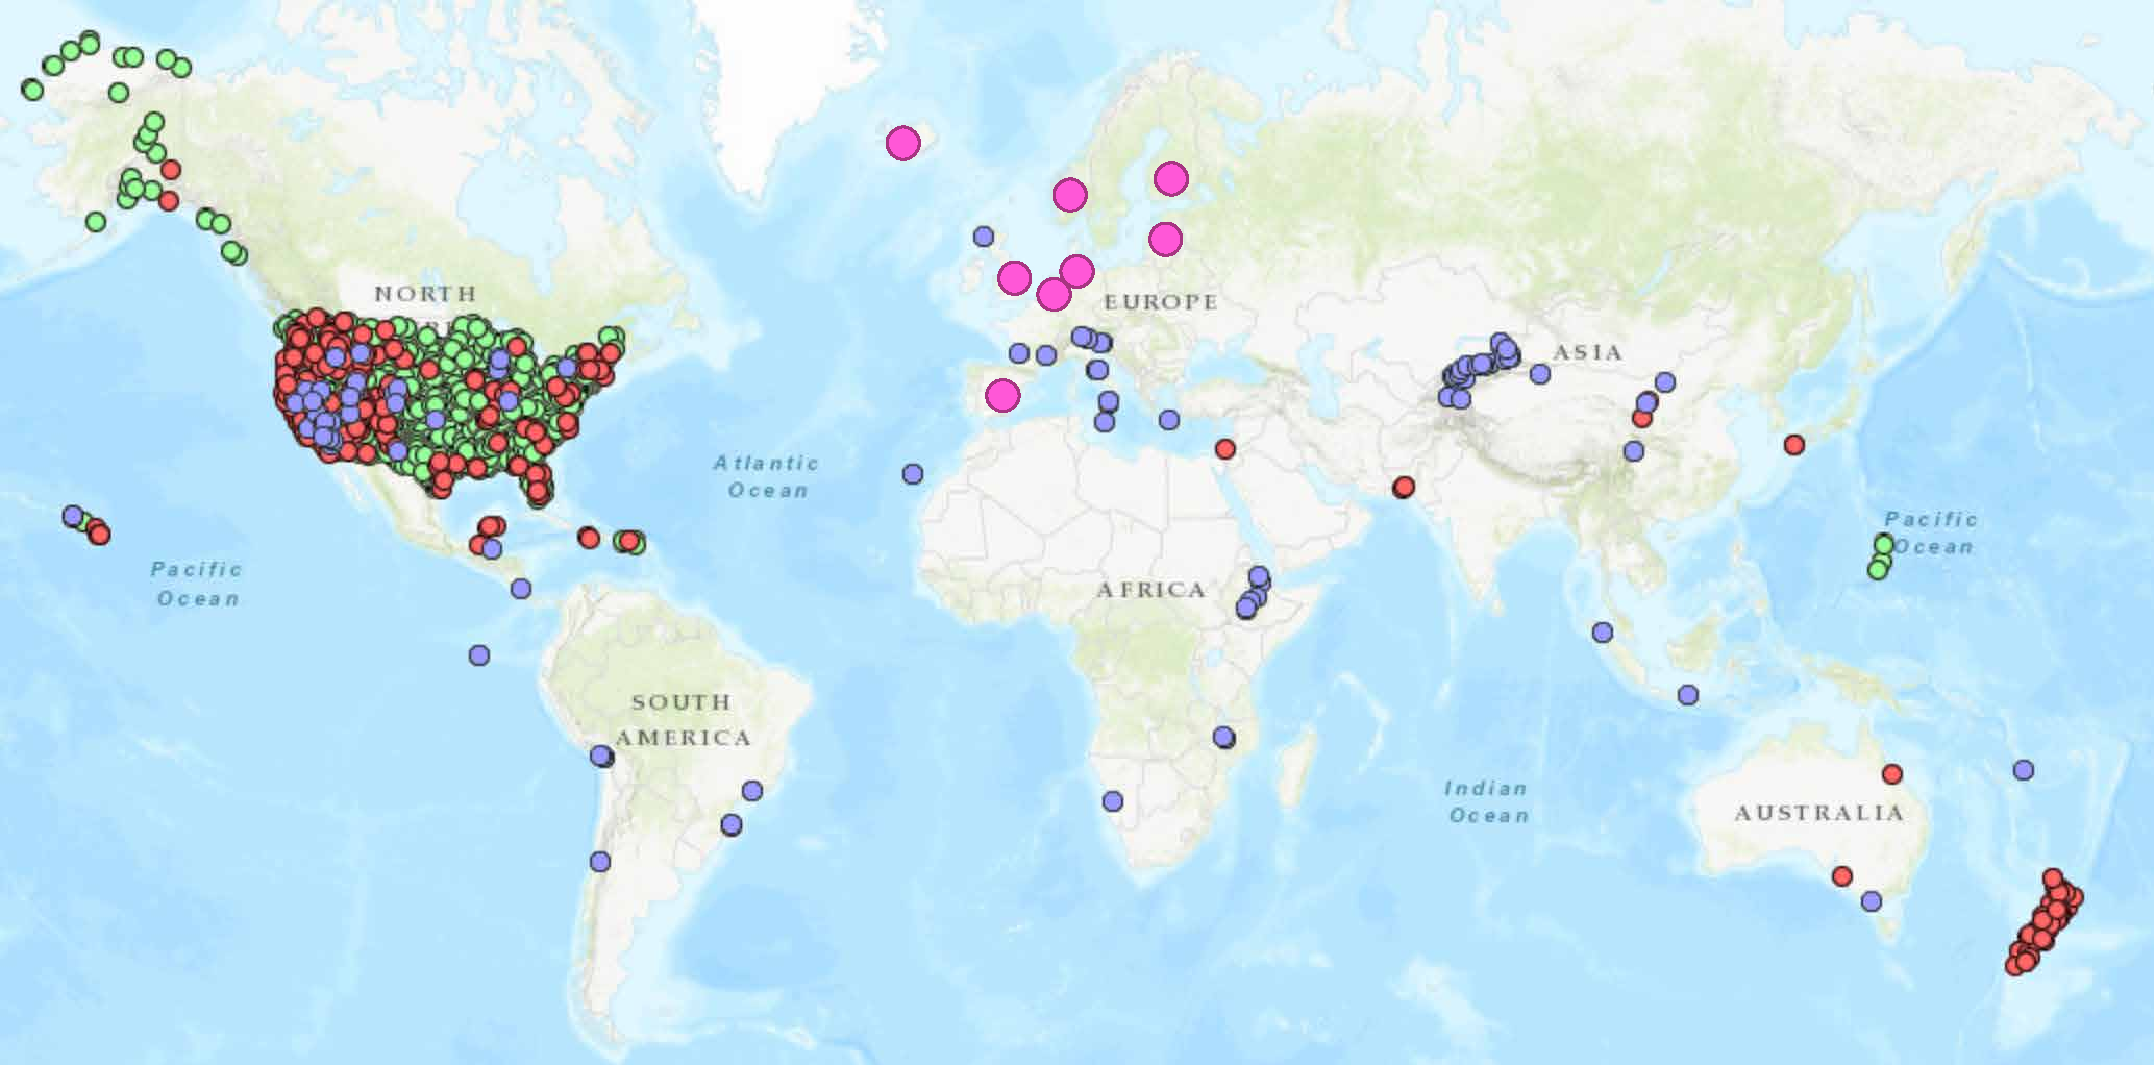
\includegraphics[width=\linewidth]{opentopography.pdf}
  \caption{OpenTopography coverage with some European datasets added in pink; there are in fact more European datasets but there is no global registry for them.}%
  \label{fig:dem_coverage}
\end{figure}

%

Global DEMs enable us to perform \emph{global} environmental studies, such as geological studies, hydrological modelling, ecosystems dynamics, the understanding of volcanic processes, and flow simulations (see Chapter~\ref{chap:runoff}).

%

While gDEMs are elevation models like local ones (and can be modelled with essentially the same formats and tools as local ones), they have several properties and characteristics that apply only to them, and we report in this chapter on the main ones.

% We first describe global acquisition techniques, then we discuss the properties (and errors and biases, etc.) that the datasets collected will have,


%%%%%%%%%%%%%%%%%%%%
%
\section{Acquisition of global elevation data}[Acquisition of global data]

The acquisition of gDEMs requires the use of a sensor mounted on a satellite.
The three most used instruments to collect elevation information are:
\begin{enumerate}
  \item Photogrammetry from optical satellite images
  \item Interferometric synthetic-aperture radar (InSAR)
  \item Lidar
\end{enumerate}


%%%
\subsection{Photogrammetry from high-resolution satellite images}

See Section~\ref{sec:photogrammetry}.


%%%
\subsection{InSAR}%
\index{InSAR}

The first gDEM (SRTM v1) was collected with InSAR in 2000, aboard the Space Shuttle Endeavour.
As InSAR requires two images of the same area for stereoscopy to derive a DEM, the Shuttle was equipped with two antennas, one in the payload bay, and one on a mast protruding \qty{60}{m} from the Shuttle.

Similarly, the TerraSAR-X satellite was joined by TanDEM-X in 2010, a twin satellite orbiting only a few hundred meters (!) away, to generate InSAR data in a single pass.

See Section~\ref{sec:insar} for more information.


%%%
\subsection{Spaceborne lidar (ICESat-2 + GEDI)}%
\index{spaceborne lidar}\index{lidar}

Spaceborne lidar is a relatively new technique, and has not yet been used to produce a gDEM\@.
We still include it here because it enables \emph{terrain} elevation measurements globally (vegetation can be filtered out), and we believe it will help us create gDEMs in the near future.

%

Lidar was first used in space on the Apollo missions, and with further technological developments, it has been used extensively from the 1990s onwards.
For example, Mercury, Mars, near-Earth asteroids, and lately again the Moon have been scanned using lidar.
Earth surface elevation lidar measurements have also been developed, often flown on the Space Shuttles.
ICESat was the first Earth-based lidar satellite, launched in 2003, with the primary goal of ice sheet monitoring.
It had an elevation accuracy of several cm and was operational for five years.
Most recently, NASA launched in 2018 two missions measure the elevation of the Earth globally with lidar instruments:

\begin{itemize}
  \item \textbf{ICESat-2}
        \marginnote{\url{https://icesat-2.gsfc.nasa.gov/}}\index{ICESat-2}
        (Ice, Cloud, and Land Elevation Satellite-2) is in a low Earth and polar orbit to investigate ice sheets, it covers the Earth between \ang{-88} and \ang{88} latitude.
        Its instrument to measure altimetry is called \emph{Advanced Topographic Laser Altimeter System} (ATLAS).
        Apart from terrain retrieval, ICESat-2 also measures the surface, such as canopy height, and has many other applications such as measuring bathymetry and estimating biomass.
  \item \textbf{GEDI}
        \marginnote{\url{https://gedi.umd.edu/}}\index{GEDI}
        (Global Ecosystem Dynamics Investigation) is attached to the international space station (ISS) and its primary goal is to investigate global ecosystems.
        It does not have global coverage since it collects measurements only between \ang{51.6} N and \ang{51.6} S.
        GEDI has been combined with TanDEM-X data to produce biomass estimates and with Landsat imagery to produce a global canopy height map.
\end{itemize}
\begin{figure}
  \centering
  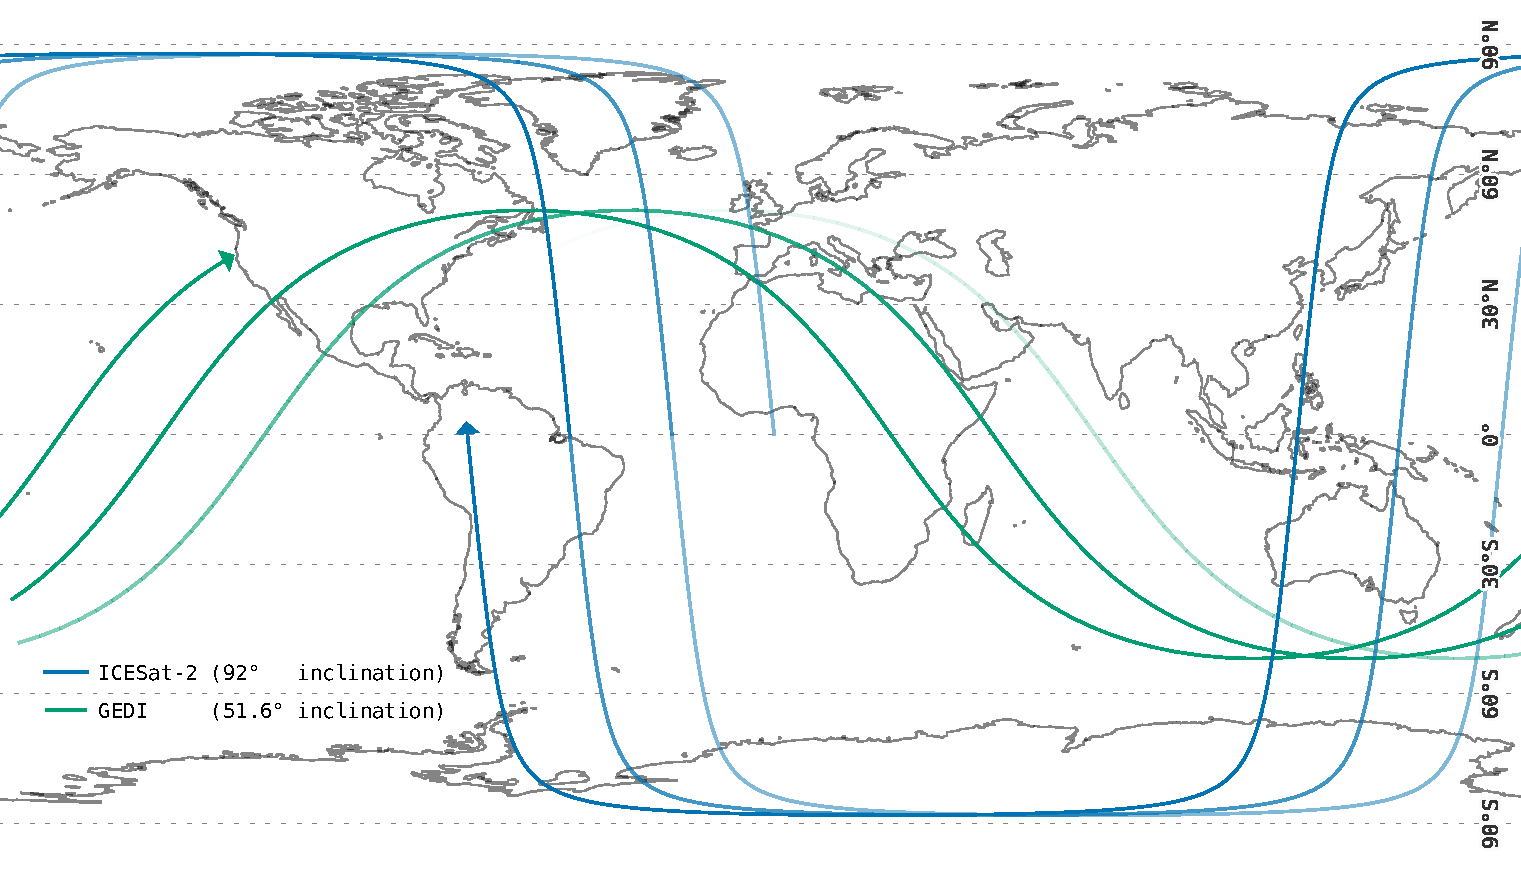
\includegraphics[width=\linewidth]{orbit}
  \caption{Ground tracks for three successive orbits of ICESat-2 and GEDI\@. The satellite is a represented by a triangle and past orbits fade out. Note the increased density of ground tracks at the latitude of inclination, as well as the lack of coverage beyond \ang{51.6}~latitude for GEDI.}%
  \label{fig:orbit}
\end{figure}

%

The characteristics of both missions are summarised in Table~\ref{tab:lidarcomparison}
\begin{table*}
  \sisetup{detect-weight=true,detect-inline-weight=math}
  \caption{Key characteristics of GEDI and ICESat-2 missions in comparison with a typical airborne lidar mission.}
  \centering
  \begin{tabular}{l|lll}
    \toprule
                           & ICESat-2                             & GEDI                                   & airborne lidar   \\
    \midrule
    \ type                 & discrete photon                      & full waveform                          & either           \\
    \ main objective       & cryosphere monitoring                & ecosystems                             & ---              \\
    \ duration             & 2018--2024(ongoing)   & 2019--2023, 2024-(ongoing)                             & single flight(s) \\
    \ orbit inclination    & \ang{92}                             & \ang{51.6}                             & NA               \\
    \ laser pulse power    & \qty{120}{{\mu}J}/\qty{30}{{\mu}J}   & \qty{15000}{{\mu}J}/\qty{4500}{{\mu}J} & NA               \\
    \ altitude             & \qty{\sim480}{km}                    & \qty{\sim420}{km}                      & \qty{0.5}{km}    \\
    \ beam footprint       & \qty{11}{m}                          & \qty{23}{m}                            & \qty{0.05}{m}    \\
    \ along track spacing  & \qty{0.7}{m}                         & \qty{70}{m}                            & \qty{0.1}{m}     \\
    \ across track spacing & \qty{3}{km}/\qty{90}{m} between pair & \qty{0.6}{km}                          & \qty{0.1}{m}     \\
    \ swath width          & \qty{6.6}{km}                        & \qty{4.2}{km}                          & \qty{1}{km}      \\
    \ beam frequency       & \qty{532}{nm} (green)                & \qty{1064}{nm} (near-infrared)         & either           \\
    \ \# laser(s)          & 1                                    & 3                                      & 1                \\
    \ \# beams             & 6                                    & 4                                      & 1                \\
    \ \# ground tracks     & 6 (in 3 strong/weak pairs)                       & 8 (4 strong, 4 weak)                                    & 1                \\
    \bottomrule
  \end{tabular}%
  \label{tab:lidarcomparison}
\end{table*}

%

ICESat-2 laser split into six beams, divided into three pairs, each pair \qty{90}{m} apart and the pairs \qty{3.3}{km} apart, for a total swath width of \qty{6.6}{km}.
Along-track, it can measure each \qty{0.7}{m}, while its beam footprint is \qty{\sim11}{m}, so each measurement overlaps.
GEDI instrument has three lasers, forming 4 beams and eight tracks, each \qty{600}{m} apart, for a total swath width of \qty{4.2}{km}.
GEDI measures a point every \qty{70}{m} along-track, with a beam footprint of \qty{23}{m}.
Furthermore, whereas GEDI employs a full-waveform laser at a typical near-infrared wavelength of \qty{1064}{nm}, ICESat-2 employs a single-photon LiDAR at a bathymetric ``green'' wavelength of \qty{532}{nm}.


%%%
\paragraph{Product levels.}
The data from the ICESat-2 and GEDI missions is made publicly available in several data products, categorised in 3 levels (Level 1, 2, and 3 data products), where a higher-level is derived from a lower-level product.
\begin{enumerate}
  \item \textbf{Level 1} products contains the raw telemetry;
  \item \textbf{Level 2} products contain directly usable geolocated data to which several corrections---such as accounting for atmospheric effects---are applied.
  \item \textbf{Level 3} data are aggregated versions of Level 2 products, which are smaller in filesize and easier to process.
        ICESat-2 differentiates between a Level 3A, which are aggregated Level 2 data products per \emph{granule}, and a Level 3B, which are gridded versions of the aggregated Level 3A data products.
        GEDI's Level 3 data product are gridded versions of Level 2 data products, like ICESat-2's Level 3B.
        GEDI also has Level 4 data products, which are model outputs---like carbon estimates---based on Level 2 data.
\end{enumerate}


%%%
\paragraph{Comparison to typical airbone lidar.}

These space borne lasers also differ considerably from airborne lasers, most notably so in their platform, resulting in significant differences in beam footprint and ground coverage.
The altitude increase results in a wider beam footprint, from \qty{\sim0.5}{m} (at \qty{500}{m}) for airborne platforms to \qty{\sim15}{m} for space platforms.
Although much wider, it is a small increase compared to the increase in altitude, going from \qty{0.5}{km} to \qty{500}{km}.
A comparison is given in Table~\ref{tab:lidarcomparison}.
Airborne LiDAR often focuses on maximizing coverage (\unit{points/m^2}) of smaller areas, whereas the coverage for space lasers is the ground track of the satellite.
While both ICESat-2 and GEDI employ instruments with multiple (split) laser beams, including the ability to point the laser away from the ground track, all to maximize coverage, this still results in very sparse and uneven coverage as shown in Figure~\ref{fig:beams}.
\begin{figure}
  \centering
  \includegraphics[width=0.8\linewidth]{tracks}
  \caption{Filtered ICESat-2 and GEDI points from a single granule each at the 47th latitude, demonstrating the beam patterns.
    Note that ICESat-2 has a smaller beam footprint and a much higher pulse repetition, but a more uneven spatial coverage than GEDI\@.
    The gaps between data here will decrease by using multiple granules, but will never disappear completely.}%
  \label{fig:beams}
\end{figure}


%%%%%%%%%%%%%%%%%%%%
%
\section{Most common products available}[Most common products]

An overview of the most common gDEMS are given in Figure~\ref{fig:gdem_inheritance}.
\begin{figure*}
  \centering
  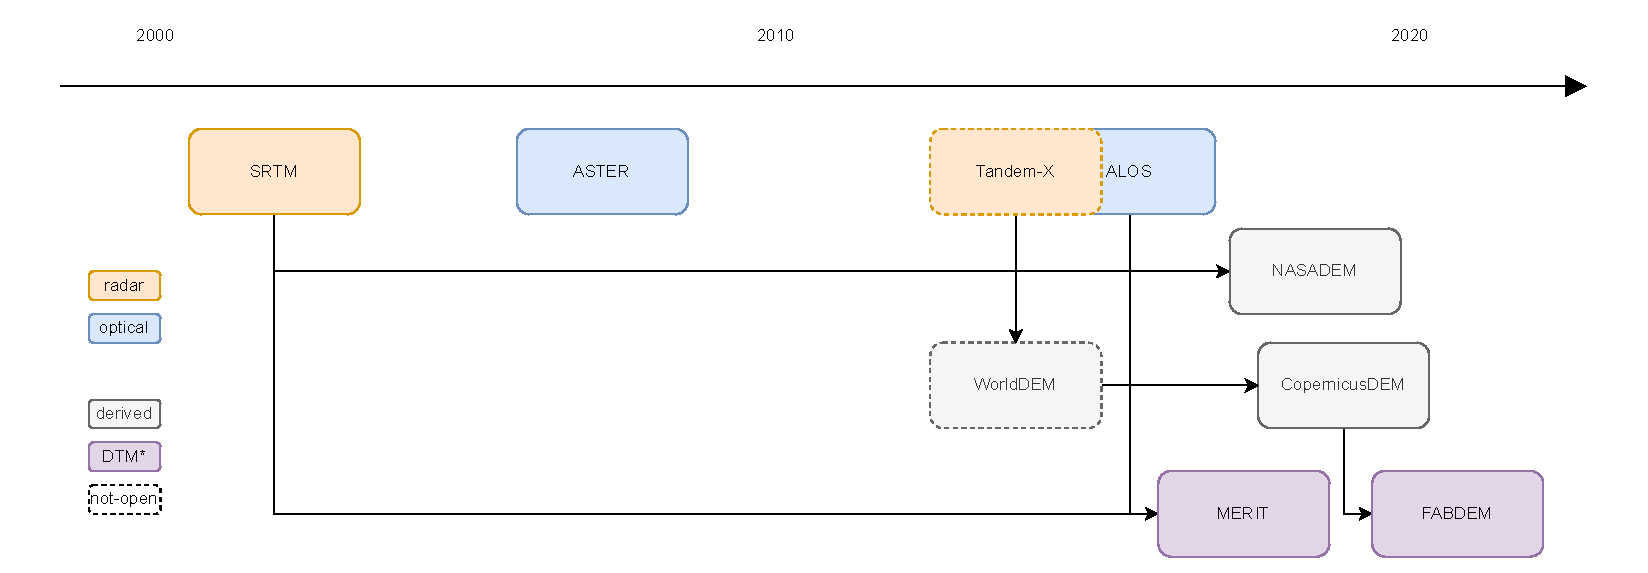
\includegraphics[width=\linewidth]{dems_overview}
  \caption{An overview of current gDEMs}%
  \label{fig:gdem_inheritance}
\end{figure*}
Note that all these products differ considerably in terms of coverage, resolution, accuracy and licensing.
Even the same product can have different versions, with different resolutions and licenses.

%

For example, SRTM is freely available, 
\marginnote{SRTM}\index{SRTM}
including its derived NASADEM, and was first introduced at \qty{90}{m}, with subsequent versions at \qty{30}{m}.
Tandem-X, and its derived WorldDEM, is a commercial product, with a resolution of \qty{\pm12}{m}.
WorldDEM-NEO, a newer version of WorldDEM with more Tandem-X data, even has a resolution of \qty{\pm5}{m}.
CopernicusDEM is a resampled WorldDEM---bought with your taxpayer money by ESA and freely distributed---at \qty{30}{m} resolution.
The pseudo DTM FABDEM (\textbf{F}orest \textbf{A}nd \textbf{B}uilding removed), while derived from the freely available CopernicusDEM, is only free for research purposes.

Similarly, while ALOS World3D is freely available at \qty{30}{m}, it also comes in a commercial version at \qty{5}{m} resolution.
There is even a \qty{0.5}{m} commercial version, based on multiple optical satellites, available on request.

% We list only the ones available as open-access?
% For instance AW3D is also available as 5m-grid, but €€€.

% Maybe we should make our own table with paid products too? Like that table: \url{https://github.com/DahnJ/Awesome-DEM#summary}
% I find it interesting to know that some products are not free, and way better


% \usepackage{booktabs}
\begin{table*}[]
  \begin{tabular}{@{}lclllll@{}}
    \toprule
                  & Year released & By                 & Sensor  & Type               & License & Resolution \\
    \midrule
    SRTM          & 2001          & NASA               & InSAR   & DSM                & Open    & 30--90m    \\
    ASTER         & 2009          & NASA               & optical & DSM                & Open    & 30m        \\
    Tandem-X      & 2014          & DLR                & InSAR   & DSM                & Closed  & 12m        \\
    WorldDEM      & 2014          & Airbus             & InSAR   & DSM/DTM$^{\prime}$ & Closed  & 5--12m     \\
    ALOS          & 2016          & JAXA               & optical & DSM                & Open    & 30m        \\
    MERIT         & 2017          & \citet{Yamazaki17} & InSAR   & DTM$^{\prime}$     & Open    & 90m        \\
    NASADEM       & 2019          & NASA               & InSAR   & DSM                & Open    & 30m        \\
    CopernicusDEM & 2020          & ESA                & InSAR   & DSM                & Open    & 30--90m    \\
    FABDEM        & 2022          & \citet{Hawker22}   & InSAR   & DTM$^{\prime}$     & Closed  & 30m        \\
    \bottomrule
  \end{tabular}
  \caption{Overview of global DEMS, see Figure~\ref{fig:dem_comparison} for their lineage.}%
  \label{tab:gdem_overview}
\end{table*}

% TODO: A few words about fusion? [Okolie22] has very long review.

\begin{figure*}
  \centering
  \begin{subfigure}[t]
    {0.45\linewidth}
    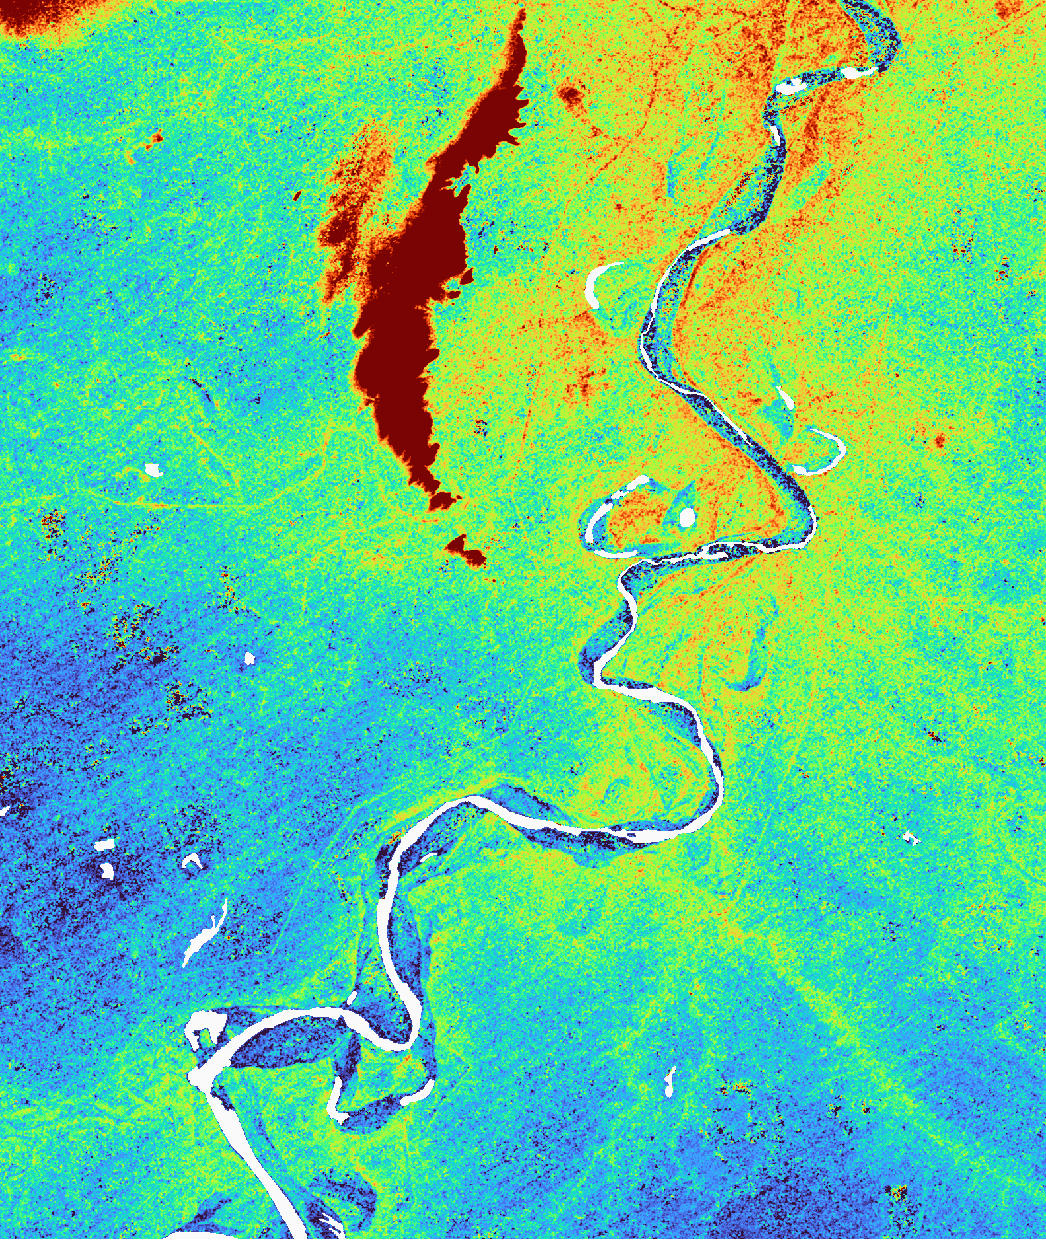
\includegraphics[width=\linewidth]{nasadem.png}
    \caption{NASADEM}\label{fig:nasadem}
  \end{subfigure}
  \qquad
  \begin{subfigure}[t]
    {0.45\linewidth}
    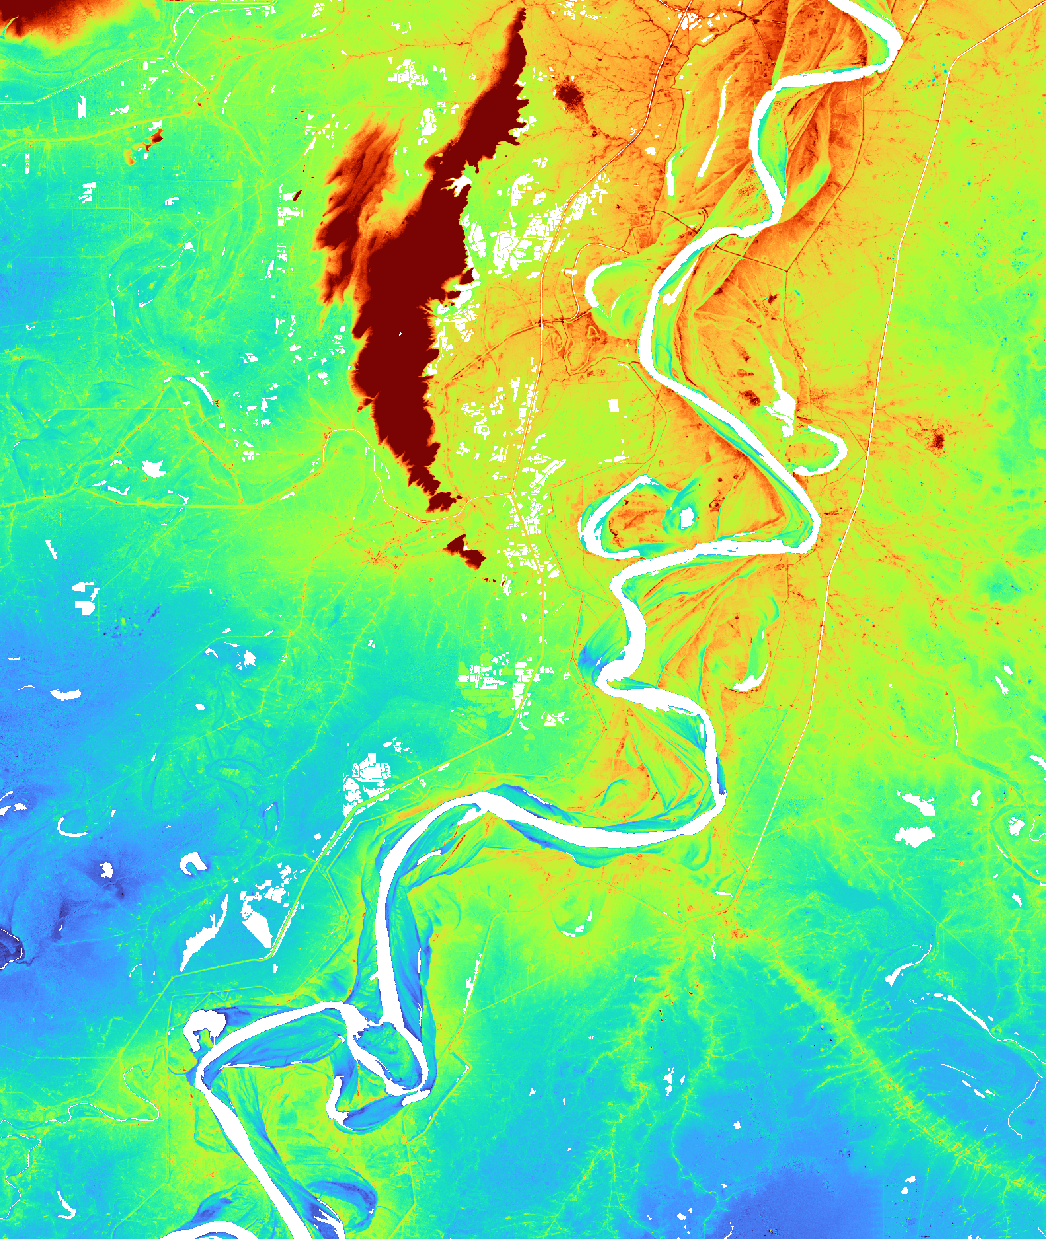
\includegraphics[width=\linewidth]{copernicusdem.png}
    \caption{CopernicusDEM}\label{fig:copernicusdem}
  \end{subfigure}
  \caption{NASADEM and CopernicusDEM for the Indus delta in Pakistan. Note the striped noise in NASADEM, and how CopernicusDEM has more detail. There is $\sim$twelve years between these images.}%
  \label{fig:dem_comparison}
\end{figure*}





%%%%%%%%%%%%%%%%%%%%
%
\section{Specific characteristics of gDEMs}[Specific characteristics]

%%
\subsection{Global often means near-global}

The data collected depend on the orbit of the satellite.
Some satellites have a polar orbit and can therefore completely measure the Earth (ICESat-2 is one example, see~\ref{fig:orbit}), while some will cover only certain latitudes (\eg\ GEDI, see~\ref{fig:orbit}).

Similarly, while the Tandem-X mission produced a DEM with a global coverage, the SRTM DEM was measured from the Space Shuttle and only covers up to \qty{60}{\degree} latitude.

%%
\subsection{Format}

The formats used to store and exchange DEMs have historically been defined by the military, which are still used by many government agencies.
One example is the \emph{Digital Terrain Elevation Data} (DTED) format, developed in the 1970s, which stores elevation in integers (which tells us a lot about the accuracy and precision possible 50 years ago).
It specifies several possible \emph{levels} in terms of resolution (in arcseconds), from level 0 at \qty{\pm1}{km} to level 2 at \qty{30}{m}.
More recently, in 2016, the Defence Gridded Elevation Data (DGED) has been defined, specifying more levels to higher resolutions and allowing GeoTIFFs to used (which removes the integer constraint).
\marginnote{GeoTIFF}
DGED also defines the structure and the specific tiling of the data at higher latitudes, as resolutions in arcseconds become smaller near the poles.

%
Most of the gDEMS are tiled in a similar way.
CopernicusDEM---adhering to the DGED level 3 standard---has tiles of 3601$\times$3601 pixels on the equator, but 3600$\times$2400 (height, width) pixels at \qty{50}{\degree} latitude, 3600$\times$1800 at \qty{60}{\degree} latitude, 3600$\times$1200 at \qty{70}{\degree} latitude, becoming as small as 3600$\times$360 for the last 5 degrees of latitude.
This tiling scheme results in pixels being as square as possible, but makes it hard to work with tiles from different latitudes.

In this context it becomes clear that the resolution should not be discussed in terms of meters, but terms of degrees (or divisions of a degree).
As the Earth has a circumference of \qty{\pm40000}{km} (measured around the Equator), \ang{1} of latitude is \qty{\pm111}{km} and \ang{1} of longitude is $111\cos\phi$ \unit{km} at latitude $\phi$.
Degrees are further divided into 60 arcminutes (\lq), which themselves are divided into 60 arcseconds (\lq\lq).
In practice, the highest resolution for SRTM (\qty{30}{m}) is actually \ang{;;1}, and its \qty{90}{m} product has a resolution of \ang{;;3}.
DTED level 0 thus has a resolution of \ang{;;30}, while level 2 has a resolution of \ang{;;1}.
%

Datasets such as SRTM and NASADEM can be provided as \texttt{.hgt} (height) files, which are not even a format, but are simply a binary file with the elevation values listed in a given order, with the geographic extent to be derived from the filename.
% GDAL can however read these files.


\begin{floatbox}
\begin{kaobox-practice}[frametitle=\faCog\ Downloading gDEMs]
Most of the gDEMS are available in a standard and easily accessible format, such as GeoTIFF\@.
However, for broad compatibility, recent advances such as new compression techniques and tiling strategies are not yet widely used.
\\ \\
One such advance is Cloud Optimized GeoTIFF (COG: \url{https://www.cogeo.org}), which is a normal GeoTIFF with a specific structure that allows it to be read piecewise from the cloud.
Without such a structure, a GeoTIFF has to be downloaded in its entirety---even if one is only interested in a small part of it---before it can be read.
\end{kaobox-practice}
\end{floatbox}

%%%
\subsection{Accuracy}

The accuracy of gDEMs is often broken down into several components and related metrics, which are not always well-defined.
The DTED and DGED specifications differentiate between horizontal and vertical accuracy, and within each defines both relative and absolute accuracy.
Relative accuracy describes the consistency of the measurements, specified as the random error component of the uncertainty between two DEM pixels. % this is related to precision
Absolute accuracy describes the total error of a measurement compared to a reference.

%

The DGED standard specifies a relative vertical accuracy of less than \qty{12}{m} for level 2 (resolution of \ang{;;1}, or \qty{\pm30}{m}) and an absolute accuracy (goal) of \qty{18}{m}.
CopernicusDEM reports a mean error of less than \qty{2}{m} for 65\% of its tiles, and another 19\% with an error of less than \qty{5}{m} in terms of absolute accuracy.


%%%
\subsection{Errors}

As with any measurements taken, gDEMs contain errors and outliers.
For example, SRTM contains a lot of noise, and has (diagonal) striping artefacts, visible in Figure~\ref{fig:nasadem} for the derived NASADEM\@.

%

Another example is CopernicusDEM that suffers from multipath errors in urban areas, which lead to small pits in the DEM, see Figure~\ref{fig:copernicus_error}.
\begin{figure*}
  \centering
  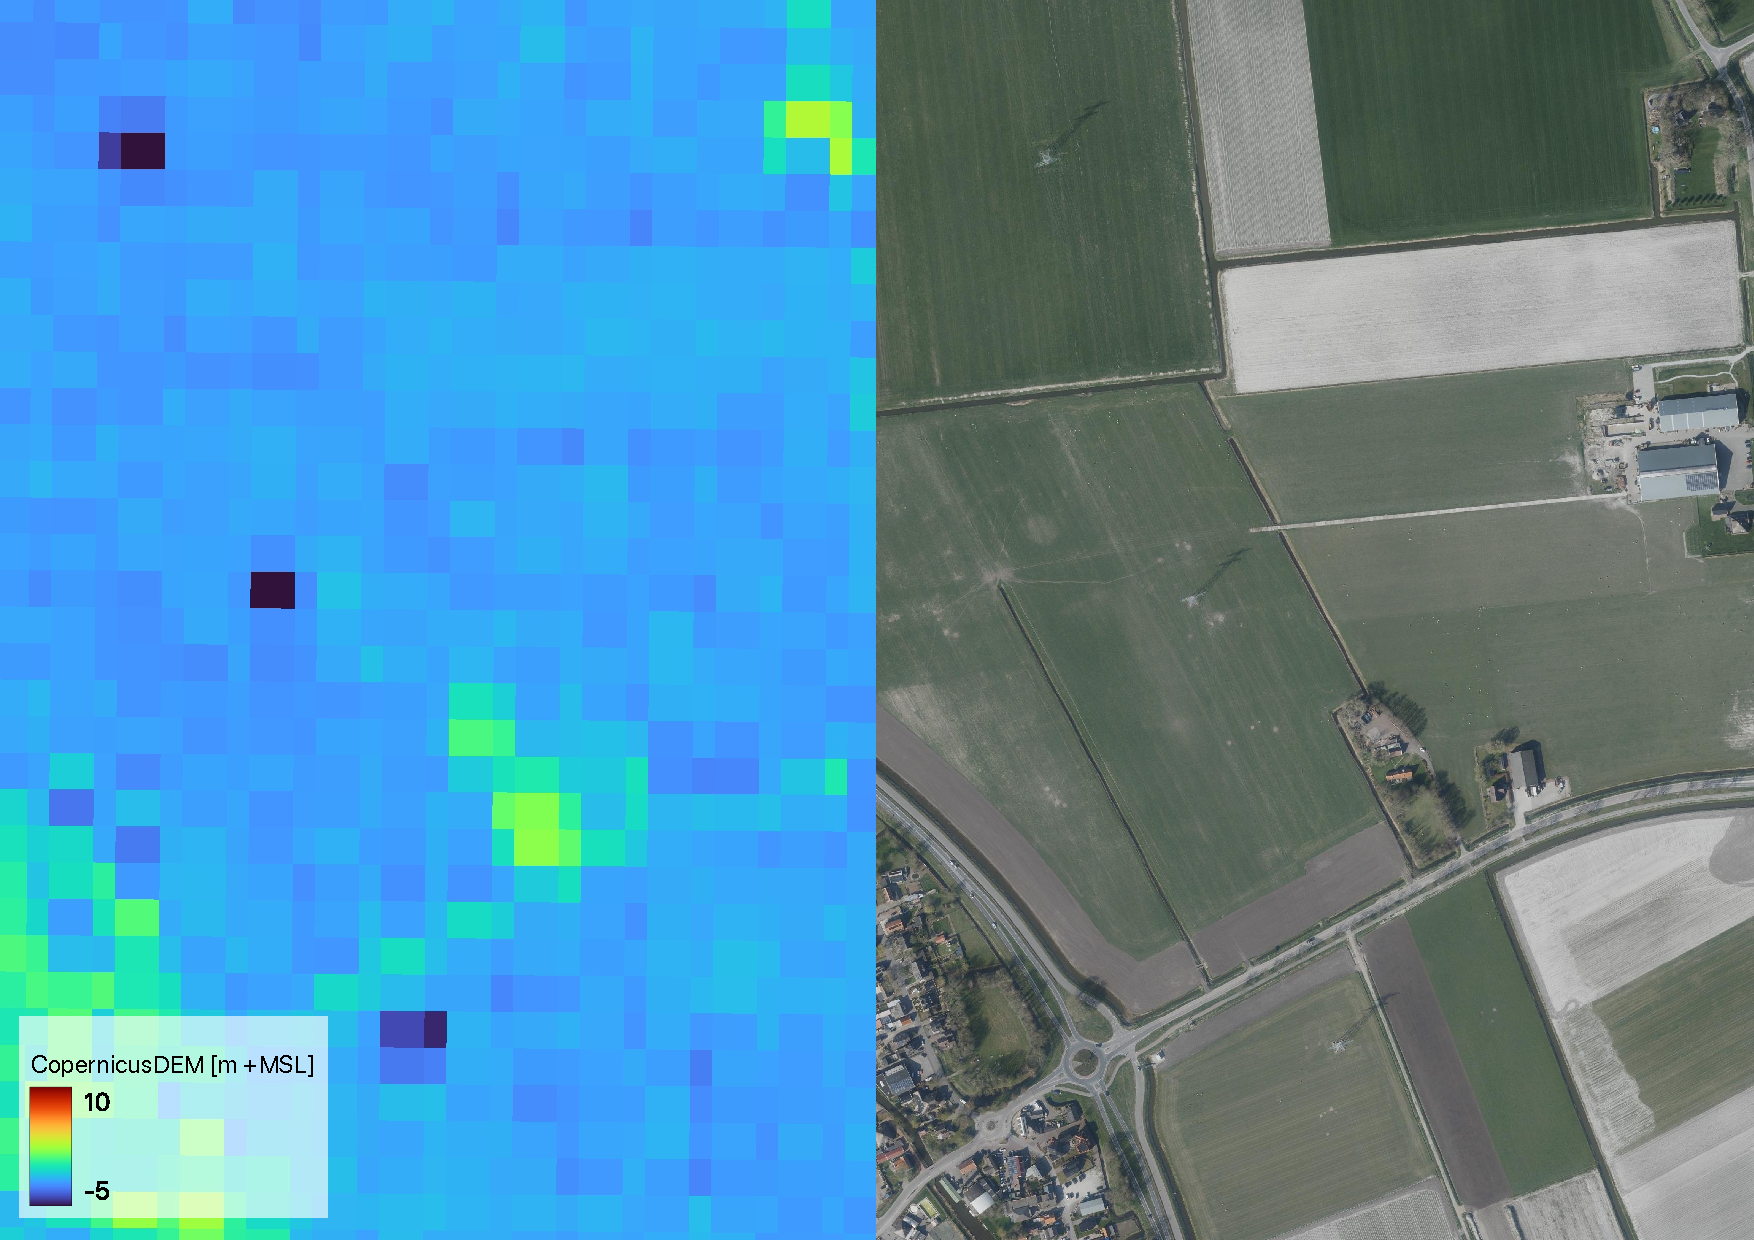
\includegraphics[width=\linewidth]{low_outliers.pdf}
  \caption{Low outliers in CopernicusDEM, with orthophoto on the right for context. Electricity poles, visible by their shadows, are the cause for these errors here.}%
  \label{fig:copernicus_error}
\end{figure*}

%

Most gDEMS suffer from voids in steep terrain, as peaks can occlude valleys below (called the shadow effect).
%%\paragraph{void filling: \url{https://en.wikipedia.org/wiki/Shuttle_Radar_Topography_Mission#Void-filled_SRTM_datasets}
\marginnote{voids in DEMs}
These voids are often filled not only by interpolation, but with the help of other gDEMS, as they measured the same area from a different angle.

%

Furthermore, gDEM products are often accompanied by a quality layer, which indicates where data has been void-filled.
Similarly, error masks with the calculated instrument error and water masks are often provided alongside the elevation data.



%%
% \paragraph{integration with sea-level datasets}
%%
% \paragraph{accuracy affected by slope (most image-based products)}


%%
\subsection{Vertical datums}

Global DEMs are vertically referenced to a specific geoid, specifically EGM96 (EPSG:5171) for SRTM and EGM2008 (EPSG:3855) for CopernicusDEM\@.%
\marginnote{Earth Gravitational Model (EGM)}
Be aware that there is a small difference---generally less than \qty{0.5}{m}---between these versions of the EGM geoid.

% MSS = Geoid + MDT
Note that the geoid is not the same as the mean sea level (MSL),%
\index{mean sea level (MSL)}\marginnote{mean sea level (MSL)}
as it does not take into account the dynamic effects of temperature and currents.
Depending on the location, the difference between the geoid and MSL can be up to \qty{1.5}{m}.


%%
\subsection{gDEMs are DSM (more than DTM)}

In contrast to local DEMs, which are often provided as either a classified point cloud, or as separate raster DSMs and DTMs, gDEMs should be classified as DSMs.
The current measurement techniques will measure the top of canopy and buildings, and not the ground below.
This is the largest source of error in gDEMS, and can considerably limit the applicability of the data.

%

Several attempts have been made to correct gDEMS for vegetation and buildings, leading to what we denote as a \emph{pseudo DTM} (DTM$^{\prime}$).
\marginnote{DTM$^{\prime} =$ pseudo DTM}
While these methods improve the accuracy of gDEMs considerably, they are not perfect, and resulting terrain still contain vegetation and/or buildings.
Recent work has also suggested that while these datasets have improved vertical accuracy, the accuracy of derived geomorphometric parameters such as slope and curvature suffers.
% are still far removed from a local DTM\@.

%
Space lidar is promising as a source to reconstruct gDEMs because lidar penetrates vegetation, and thus obtaining a DTM is an easier process.
Recently, several global \emph{coastal} pseudo DTMs---covering only areas near or below sealevel---have been produced using space lidar (to some extent): CoastalDEM~\citep{kulpCoastalDEMV30Improving}, DiluviumDEM~\citep{dusseauDiluviumDEMEnhancedAccuracy2023} and DeltaDTM~\citep{pronkDeltaDTMGlobalCoastal2024}.


%%%%%%%%%%%%%%%%%%%%
%
\section{Notes and comments}

% TODO: add some papers to read here

\citet{Yang11} provide a detailed list of applications where gDEMs (SRTM, but when the paper was written (2011) SRTM was still the main product available globally) are necessary as input.

\citet{Schumann2018} make a case for the need for high-accuracy open-access DEMs, demonstrating SRTM is not good enough for many applications.

\citet{Hancock2021} investigates the requirements for a global lidar DEM\@.

Further reading about DEM terminology can be found in \citet{Guth2021}, which is one of the products of the \emph{Digital Elevation Model Intercomparison eXperiment} (DEMIX) group.
They also published a paper comparing the vertical accuracy and derived parameters of several gDEMs~\citep{guthRanking10Global2024}.

Arguably the best place to download DEMs (gDEMS, local ones, lidar datasets, etc.) is OpenTopography (\url{https://opentopography.org}).
Otherwise each gDEM has its own download portal, with its own registration systems and its specific ways of searching and downloading the data.
In case of the most recent gDEMS, such as CopernicusDEM, the data must be downloaded as \texttt{.tar} (archives) for \ang{1}$\times$\ang{1} tiles via FTP, in folders for each continent and then country.
Data is duplicated for the border areas, totalling \qty{2}{TB}.

To learn more about the DGED format, read \url{https://dgiwg.org/documents/dgiwg-standards}.
Similarly, reading a user guide on any of the gDEMS is a good idea, such as the one for \href{https://spacedata.copernicus.eu/documents/20126/0/GEO1988-CopernicusDEM-SPE-002_ProductHandbook_I3.0+%281%29.pdf}{CopernicusDEM Product Handbook}.

\citet{Hawker22} give the details how the vegetation and buildings are removed from CopernicusDEM to create FABDEM\@.

%%%%%%%%%%%%%%%%%%%%
%
\section{Exercises}

% TODO: think of some exam questions to put here
\begin{enumerate}
  \item How wide is 1 degree longitude at the latitude where the city of Delft is? And at the North Pole?
  \item How old is the oldest gDEM, and what latitudes did it cover?
  \item Assume you want to compare the elevations from AHN5 to those of CopernicusDEM\@. Which steps/conversions are needed?
\end{enumerate}
                   %- 03
%!TEX root = ../terrainbook.tex

\graphicspath{{dtvd/}}


\newcommand{\Orient}{O\textsc{rientation}\xspace}
\newcommand{\walk}{W\textsc{alk}\xspace}
\newcommand{\Incircle}{I\textsc{n}C\textsc{ircle}\xspace}

\chapter{Triangulations \& Voronoi diagrams}%
\label{chap:dtvd}

% TODO : introduction to the chapter: DT and VD are fundamental structures in terrains, both for representation but also for processing (interpolation and many other operations with terrains and point clouds)


\section{The Voronoi Diagram}

Let $S$ be a set of points in $\mathbb{R}^2$ (the two-dimensional Euclidean space). 
The Voronoi cell of a point $p \in S$, defined $\mathcal{V}_{p}$, is the set of points $x \in \mathbb{R}^2$ that are closer to $p$ than to any other point in $S$; that is:
\begin{equation}
\mathcal{V}_p = \{x \in \mathbb{R}^{2} \ | \ \|x-p\| \, \leq \, \|x-q\|, \ \forall \, q \in S \}. 
\end{equation}
The union of the Voronoi cells of all generating points $p \in S$ form the Voronoi diagram of $S$, defined VD($S$). 
If $S$ contains only two points $p$ and $q$, then VD($S$) is formed by a single line defined by all the points $x \in \mathbb{R}^2$ that are equidistant from $p$ and $q$. 
This line is the perpendicular bisector of the line segment from $p$ to $q$, and splits the plane into two half-planes. 
$\mathcal{V}_p$ is formed by the half-plane containing $p$, and $\mathcal{V}_q$ by the one containing $q$. 
As shown in Figure~\ref{fig:halfspaces}a,
\begin{figure}
  \centering
  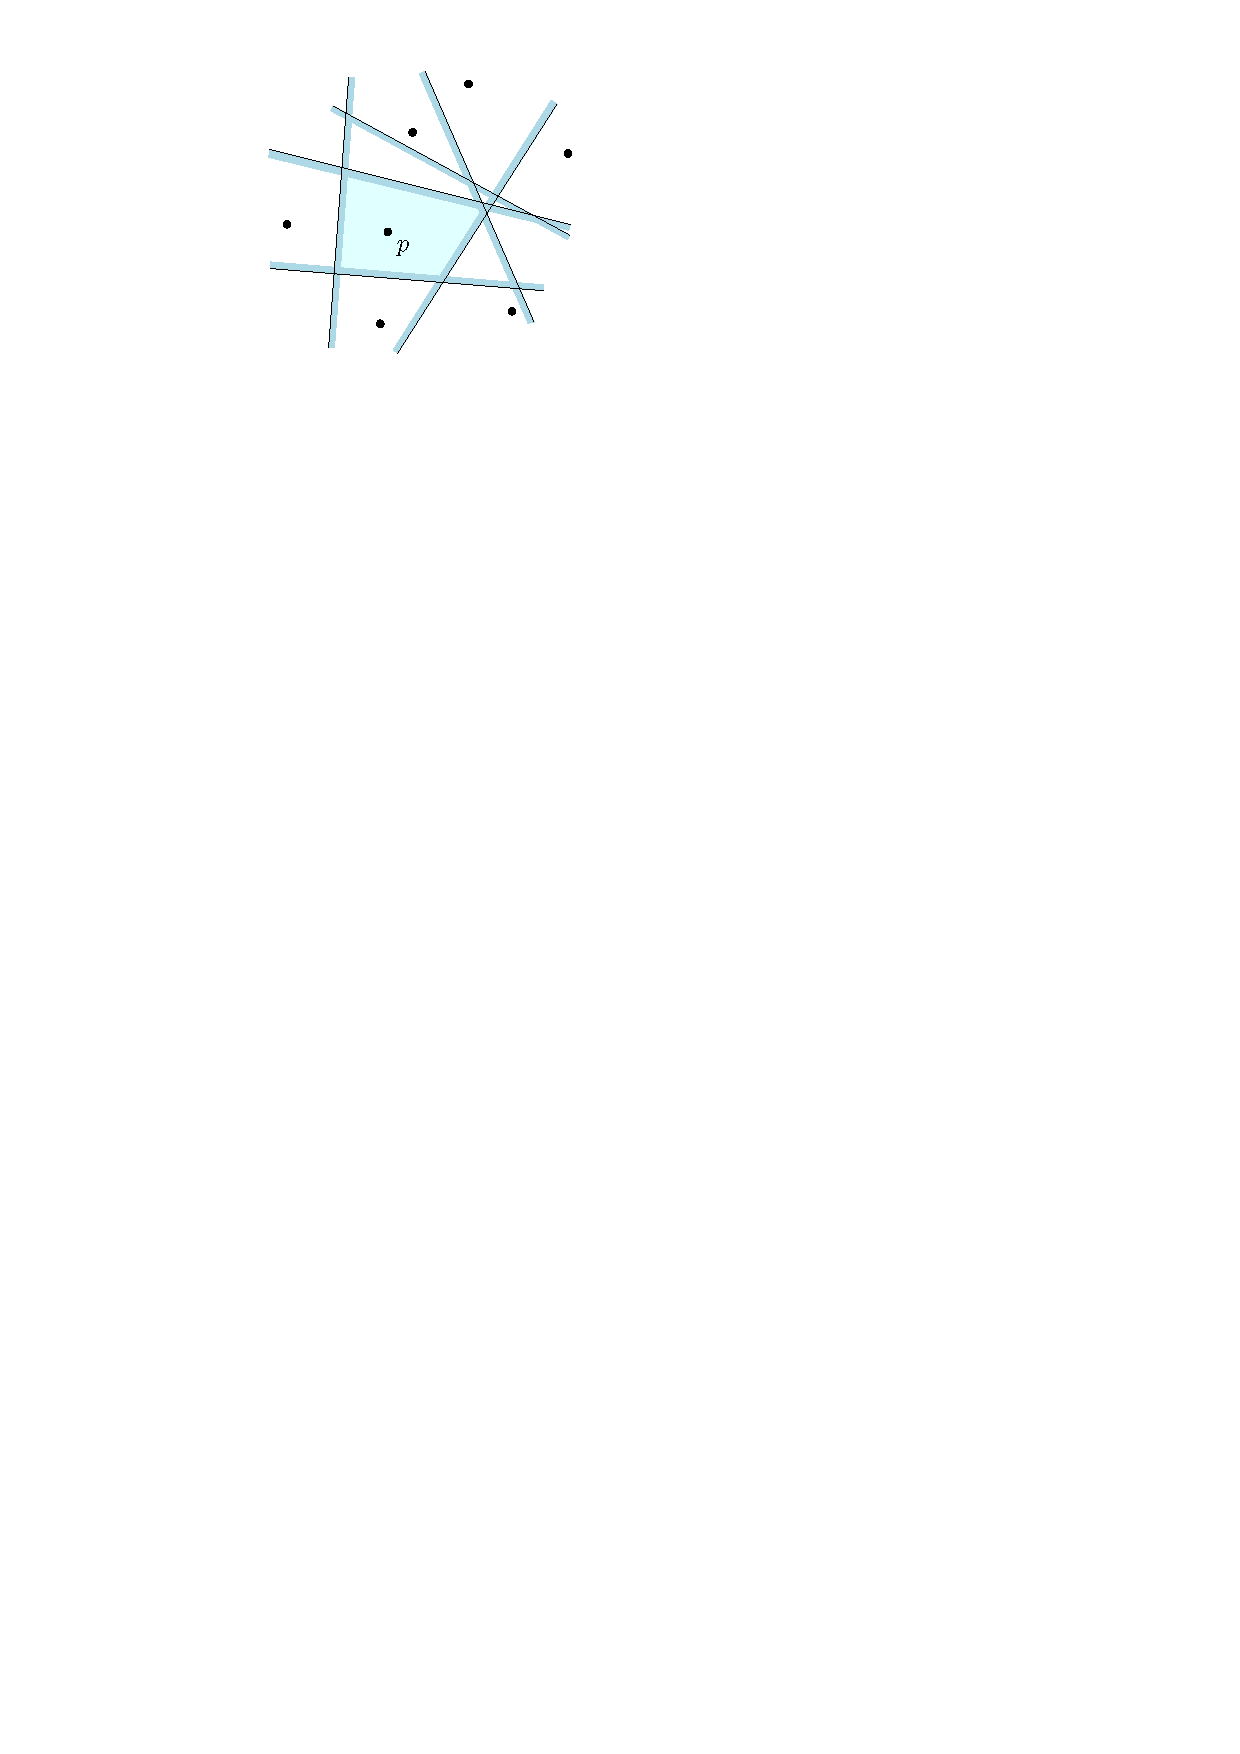
\includegraphics[width=0.6\textwidth]{figs/halfspaces}
  \caption{\textbf{(a)} The Voronoi cell $\mathcal{V}_p$ is formed by the intersection of all the half-planes between $p$ and the other points. \textbf{(b)} The VD for a set $S$ of points in the plane (the black points). The Voronoi vertices (white points) are located at the centre of the circle passing through three points in $S$, provided that this circle contains no other points in $S$ in its interior.} 
\label{fig:halfspaces}
\end{figure}
when $S$ contains more than two points (let us say it contains $n$ points), the Voronoi cell of a given point $p \in S$ is obtained by the intersection of $n-1$ half-planes defined by $p$ and the other points $q \in S$. 
That means that $\mathcal{V}_{p}$ is always convex. 
Notice also that every point $x \in \mathbb{R}^2$ has at least one nearest point in $S$, which means that VD($S$) covers the entire space.

%

As shown in Figure~\ref{fig:halfspaces}b, the VD of a set $S$ of points in $\mathbb{R}^2$ is a planar graph. 
Its edges are the perpendicular bisectors of the line segments of pairs of points in $S$, and its vertices are located at the centres of the circles passing through three points in $S$. 
The VD in $\mathbb{R}^2$ can also be seen as a two-dimensional cell complex where each 2-cell is a (convex) polygon (see Figure~\ref{fig:vd2d}). 
\begin{figure}
  \centering
  \includegraphics[page=3,width=0.6\textwidth]{figs/vd2d}
  \caption{VD of a set of points in the plane (clipped by a box). The point $p$ (whose Voronoi cell is dark grey) has seven neighbouring cells (light grey).} 
\label{fig:vd2d}
\end{figure}
Two Voronoi cells, $\mathcal{V}_{p}$ and $\mathcal{V}_{q}$, lie on the opposite sides of the perpendicular bisector separating the points $p$ and $q$. 

%

The VD has many interesting properties, what follows is a list of the most relevant properties in the context of this course.
\begin{description}
  \item[Size:] if $S$ has $n$ points, then VD($S$) has exactly $n$ Voronoi cells since there is a one-to-one mapping between the points and the cells.
  \item[Voronoi vertices:] a Voronoi vertex is equidistant from 3 data points. Observe for instance in Figure~\ref{fig:halfspaces}b that the Voronoi vertices are at the centre of circles.
  \item[Voronoi edges:] a Voronoi edge is equidistant from 2 points.
  \item[Convex hull:] let $S$ be a set of points in $\mathbb{R}^2$, and $p$ one of its points. $\mathcal{V}_{p}$ is unbounded if $p$ bounds conv($S$). Otherwise, $\mathcal{V}_{p}$ is the convex hull of its Voronoi vertices. Observe that in Figure~\ref{fig:halfspaces}b, only the point in the middle has a bounded Voronoi cell.
\end{description}
  

%%%
%
\section{The Delaunay Triangulation}
\label{sec:dt_definition}

Let $\mathcal{D}$ be the VD of a set $S$ of points in $\mathbb{R}^2$. 
Since VD($S$) is a planar graph, it has a dual graph, and let $\mathcal{T}$ be this dual graph obtained by drawing straight edges between two points $p,q \in S$ if and only if $\mathcal{V}_{p}$ and $\mathcal{V}_{q}$ are adjacent in $\mathcal{D}$. 
Because the vertices in $\mathcal{D}$ are of degree 3 (3 edges connected to it), the graph $\mathcal{T}$ is a triangulation. 
$\mathcal{T}$ is actually called the Delaunay triangulation (DT) of $S$, and, as shown in Figure~\ref{fig:dt2da}, 
\begin{figure}
  \centering
  \begin{subfigure}[b]{0.45\linewidth}
    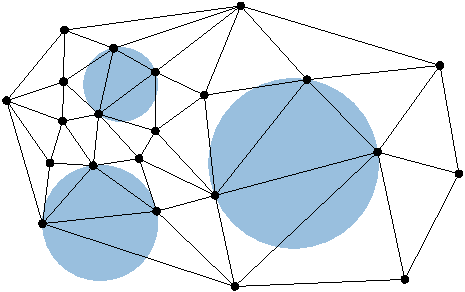
\includegraphics[width=\textwidth]{figs/dt2d_2}
    \caption{}\label{fig:dt2da}
  \end{subfigure}%
  \qquad
  \begin{subfigure}[b]{0.3\linewidth}
    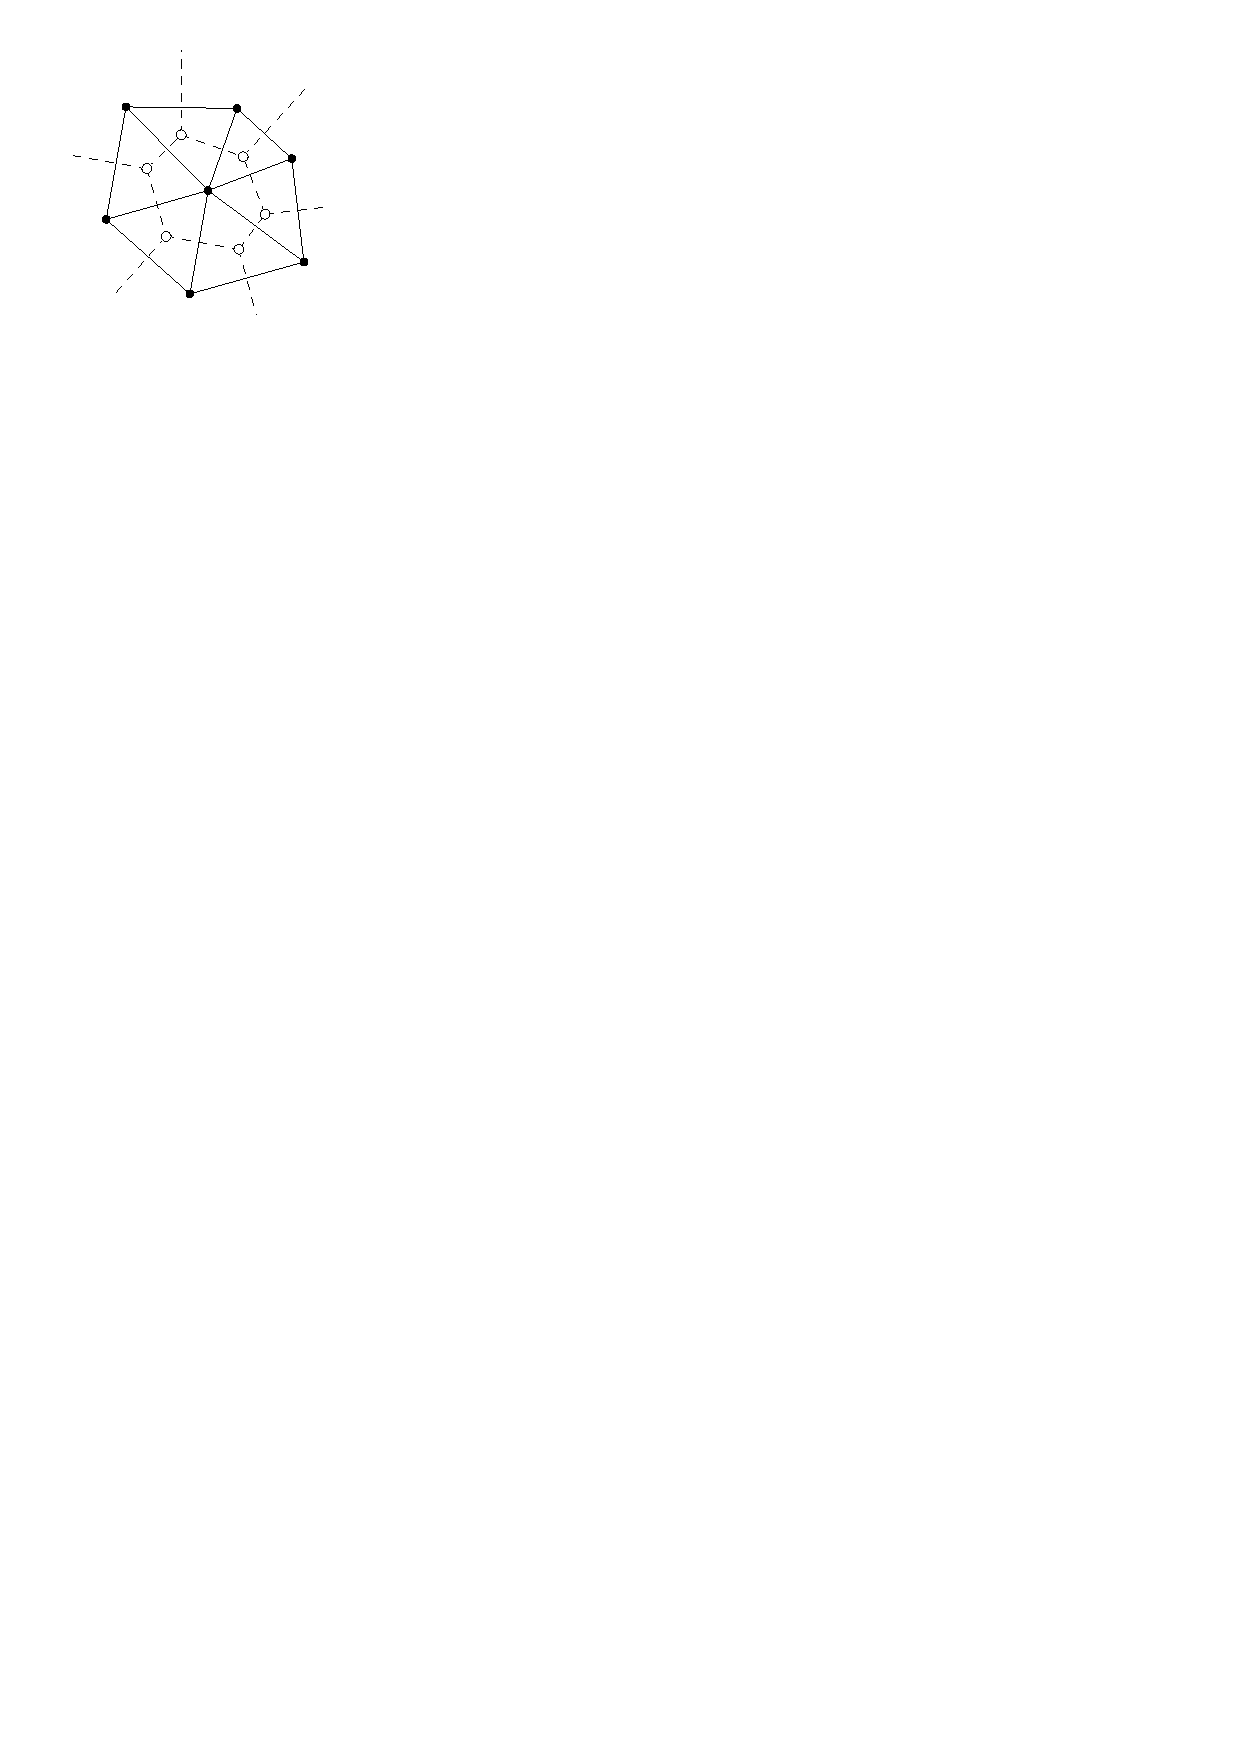
\includegraphics[width=\textwidth]{figs/duality_2d}
    \caption{}\label{fig:dt2db}
  \end{subfigure}%
  \caption{\textbf{(a)} The DT of a set of points in the plane (same point set as Figure~\ref{fig:vd2d}). \textbf{(b)} Both the DT (black lines) and the VD (dashed lines) of a set of points in the plane.}
\label{fig:dt2d}
\end{figure}
partitions the plane into triangles---where the vertices of the triangles are the points in $S$ generating each Voronoi cell---that satisfy the \emph{empty circumcircle} test (a circle is said to be \emph{empty} when no points are in its interior). 
If $S$ is in general position, then DT($S$) is unique.

%
\subsection{Convex Hull}
The DT of a set $S$ of points subdivides completely conv($S$), \ie\ the union of all the triangles in DT($S$) is conv($S$).

Let $S$ be a set of points in $\mathbb{R}^2$, the \emph{convex hull} of $S$, denoted conv($S$), is the minimal convex set containing $S$. 
It is best understood with the elastic band analogy: imagine each point in $\mathbb{R}^2$ being a nail sticking out of the plane, and a rubber band stretched to contain all the nails, as shown in Figure~\ref{fig:convex_hull}. 
\begin{figure}
  \centering
  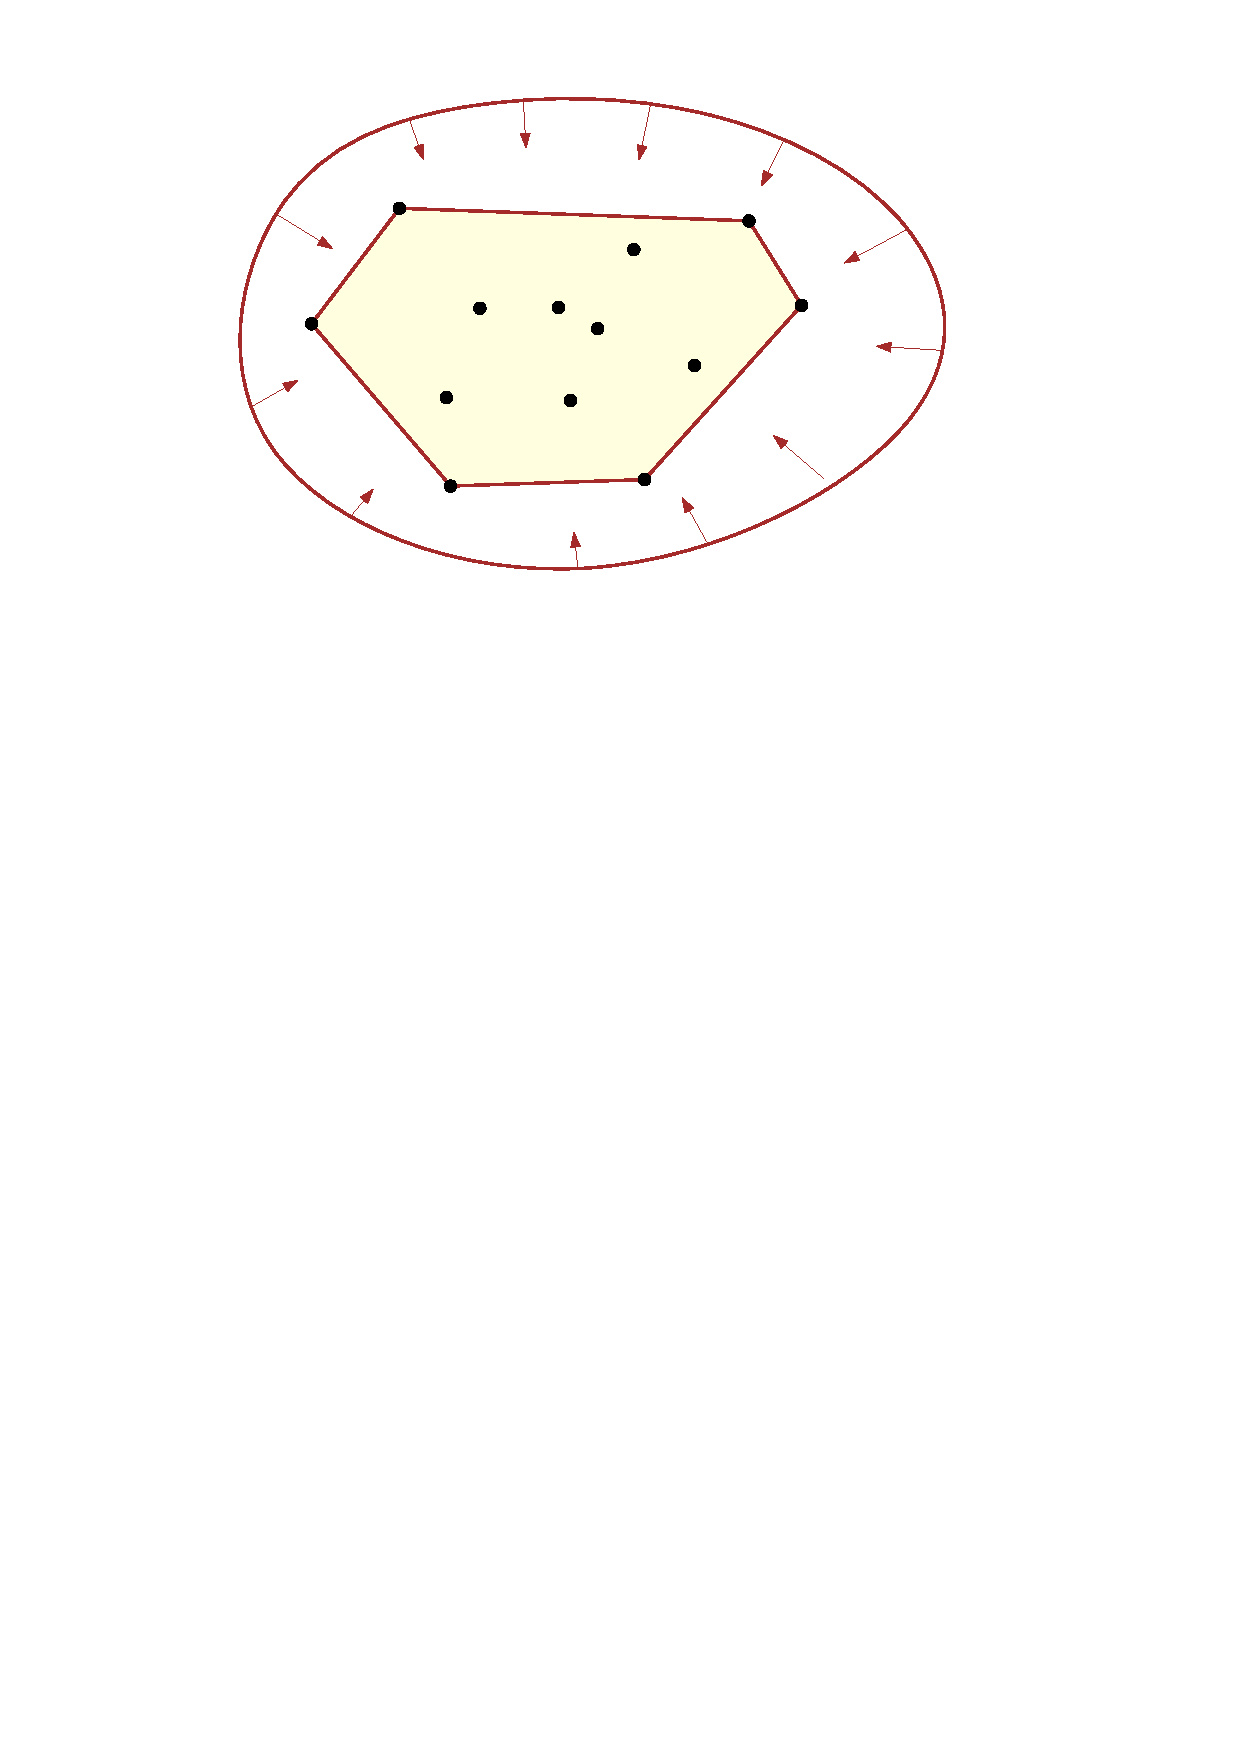
\includegraphics[width=0.35\textwidth]{figs/convex_hull}
  \caption{The convex hull of a set of points in $\mathbb{R}^2$.} 
\label{fig:convex_hull}
\end{figure}
When released, the rubber band will assume the shape of the convex hull of the nails. 
Notice that conv($S$) is not only formed by the edges connecting the points (the rubber band), but all the points of $\mathbb{R}^2$ that are contained within these edges (thus the whole polygon).


%
\subsection{Local Optimality}
Let $\mathcal{T}$ be a triangulation of $S$ in $\mathbb{R}^2$. 
An edge $\sigma$ is said to be \emph{locally} Delaunay if it either:
\begin{description}
  \item[(i)] belongs to only one triangle, and thus bounds conv($S$), or
  \item[(ii)] belongs to two triangles $\tau_a$ and $\tau_b$, formed by the vertices of $\sigma$ and respectively the vertices $p$ and $p$, and $p$ is outside of the circumcircle of $\tau_a$. 
\end{description}
The second case is illustrated in Figure~\ref{fig:local}: the triangles $abd$ and $bcd$ are Delaunay, and thus is the edge $bd$; the edge $ac$ is not Delaunay.
\begin{figure}
  \centering
  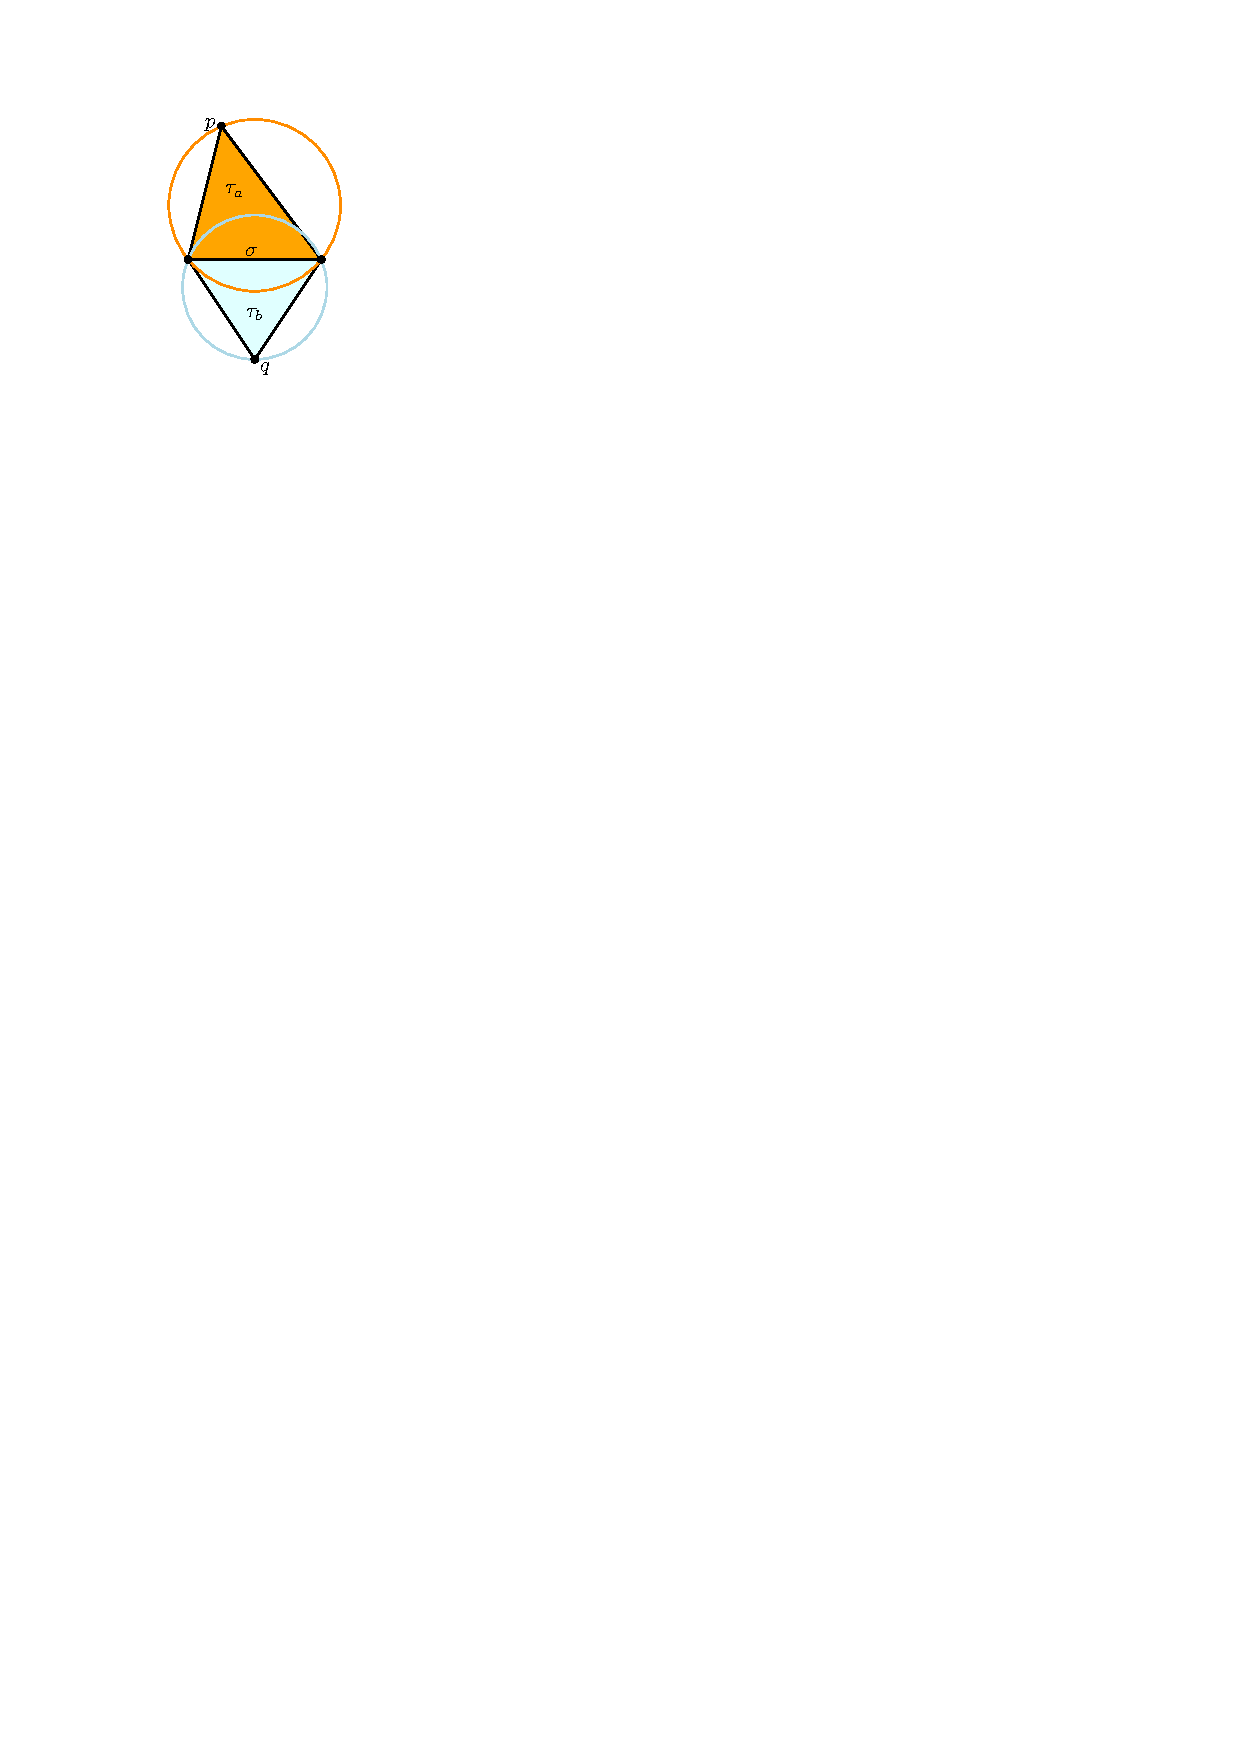
\includegraphics[width=0.7\textwidth]{figs/local}
  \caption{Only one configuration is Delaunay (the left one).} 
\label{fig:local}
\end{figure}
In an arbitrary triangulation, not every edge that is locally Delaunay is necessarily a edge of DT($S$), but local optimality implies globally optimality in the case of the DT:
\begin{quote}
  Let $\mathcal{T}$ be a triangulation of a point set $S$ in $\mathbb{R}^2$. If every edge of $\mathcal{T}$ is locally Delaunay, then $\mathcal{T}$ is the Delaunay triangulation of $S$.
\end{quote}
This has serious implications as the DT---and its dual---are locally modifiable, \ie\ we can theoretically insert, delete or move a points in $S$ without recomputing DT($S$) from scratch.


%%%
%
\subsection{Angle Optimality}
The DT in two dimensions has a very important property that is useful in applications such as finite element meshing or interpolation: the \emph{max-min angle optimality}. Among all the possible triangulations of a set $S$ of points in $\mathbb{R}^2$, DT($S$) maximises the minimum angle (max-min property), and also minimises the maximum circumradii. 
In other words, it creates triangles that are as equilateral as possible. 
Notice here that maximising the minimum angle is not the same as minimising the maximum, and the DT only guarantees the former.


%%%
\subsection{Lifting on the paraboloid}
\label{sec:parabolic_lifting}

There exists a close relationship between DTs in $\mathbb{R}^{d}$ and convex polytopes in $\mathbb{R}^{d+1}$. 

Let $S$ be a set of points in $\mathbb{R}^{d}$, and let $x_{1}, x_{2}, \ldots , x_{d}$ be the coordinates axes. 
The parabolic lifting map projects each vertex $v(v_{x1}, v_{x2}, \ldots , v_{xd})$ to a vertex $v^{+}(v_{x1}, v_{x2}, \ldots , v_{xd}, v_{x1}^{2}+v_{x2}^{2}+\cdots+v_{xd}^{2})$ on the paraboloid of revolution in $\mathbb{R}^{d+1}$. 
The set of points thus obtained is denoted $S^{+}$. 
Observe that, for the two-dimensional case, the paraboloid in three dimensions defines a surface whose vertical cross sections are parabolas, and whose horizontal cross sections are circles; the same ideas are valid in higher dimensions. 

%

The relationship is the following: every facet (a $d$-dimensional simplex) of the lower envelope of conv($S^{+}$) projects to a $d$-simplex of the Delaunay triangulation of $S$. 
This is illustrated in Figure~\ref{fig:paraboloid} for the construction of the DT in $\mathbb{R}^{2}$. 
\begin{figure}
  \centering
  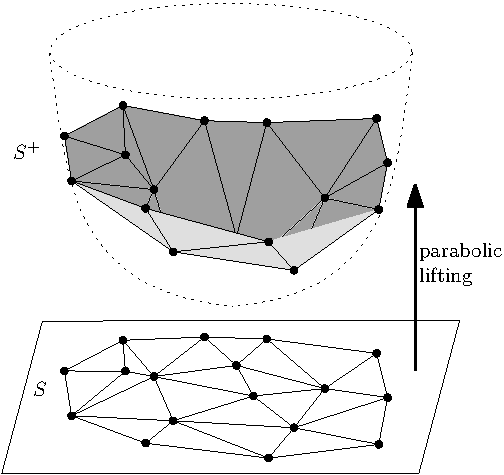
\includegraphics[width=0.4\textwidth]{figs/paraboloid}
  \caption{The parabolic lifting map for a set $S$ of points $\mathbb{R}^2$.}
\label{fig:paraboloid}
\end{figure}

%

In short, the construction of the $d$-dimensional DT can be transformed into the construction of the convex hull of the lifted set of points in ($d+1$) dimensions.
In practice, since it is easier to construct convex hulls (especially in higher dimensions, \ie\ 4+), the DT is often constructed with this method.




%%%
%
\subsection{Degeneracies}
\label{sec:degeneracies}

The previous definitions of the VD and the DT assumed that the set $S$ of points is in general position, \ie\ the distribution of points does not create any ambiguity in the two structures. 
For the VD/DT in $\mathbb{R}^{2}$, the degeneracies, or special cases, occur when 3 points lie on the same line and/or when 4 points are cocircular. 
For example, in two dimensions, when four or more points in $S$ are cocircular there is an ambiguity in the definition of DT($S$). 
As shown in Figure~\ref{fig:degeneracies},
\begin{figure}
  \centering
  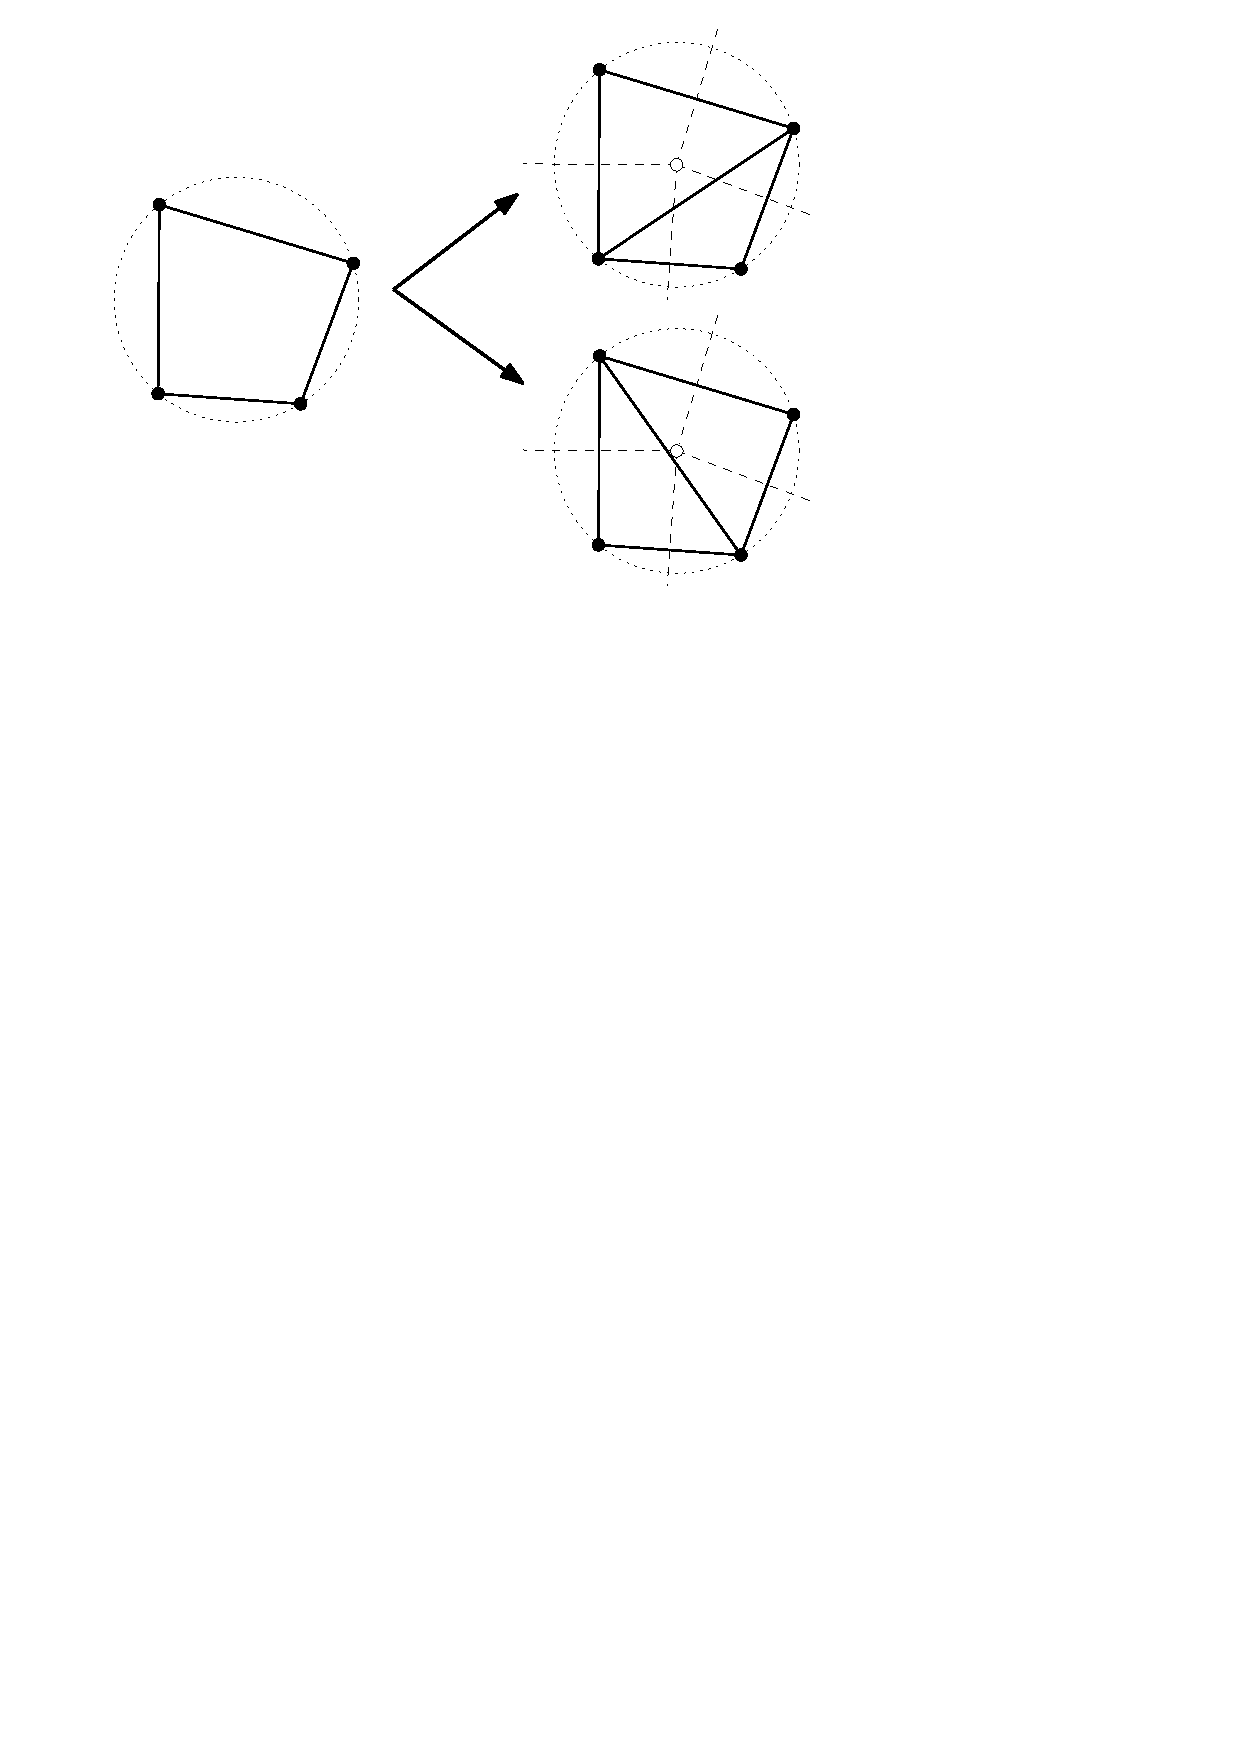
\includegraphics[width=0.4\textwidth]{figs/degeneracies}
  \caption{The DT for four cocircular points in two dimensions is not unique (but the VD is).}
\label{fig:degeneracies}
\end{figure}
the quadrilateral can be triangulated with two different diagonals, and an arbitrary choice must be made since both respect the Delaunay criterion (points should not be on the interior of a circumcircle, but more than three can lie directly on the circumcircle).

This implies that in the presence of four or more cocircular points, DT($S$) is not unique. 
Notice that even in the presence of cocircular points, VD($S$) is still unique, but it has different properties. 
For example, in Figure~\ref{fig:degeneracies}, the Voronoi vertex in the middle has degree 4 (remember that when $S$ is in general position, every vertex in VD($S$) has degree 3). 
When three or more points are collinear, DT($S$) and VD($S$) are unique, but problems with the implementation of the structures can arise.


%%%
%
\section{Duality between the DT and the VD}
\label{sec:duality}

Duality can have many different meanings in mathematics, but it always refers to the translation or mapping in a one-to-one fashion of concepts or structures. 
We use it in this course in the sense of the dual graph of a given graph. 
Let $G$ be a planar graph, as illustrated in Figure~\ref{fig:dual_graph} (black edges).
\begin{figure}
  \centering
  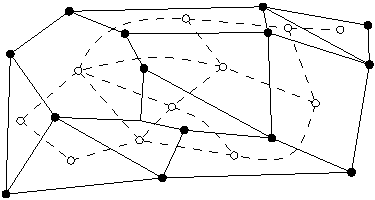
\includegraphics[width=0.45\textwidth]{figs/dual_graph}
  \caption{A graph $G$ (black lines), and its dual graph $G^\star$ (dashed lines).}
\label{fig:dual_graph}
\end{figure}
Observe that $G$ can also be seen as a cell complex in $\mathbb{R}^{2}$. 
The duality mapping is as follows (also shown in details in Figure~\ref{fig:dualdetailtab})
The dual graph $G^{\star}$ has a vertex for each face (polygon) in $G$, and the vertices in $G^{\star}$ are linked by an edge if and only if the two corresponding dual faces in $G$ are adjacent (in Figure~\ref{fig:dual_graph}, $G^{\star}$ is represented with dashed lines). 
Notice also that each polygon in $G^{\star}$ corresponds to a vertex in $G$, and that each edge of $G$ is actually dual to one edge (an arc in Figure~\ref{fig:dual_graph}) of $G^{\star}$ (for the sake of simplicity the dual edges to the edges on the boundary of $G$ are not drawn).

The VD and the DT are the best example of the duality between plane graphs.

\begin{figure}[h]
% \centering
% \setcapindent{1em}
\centering
\begin{minipage}[c]{0.4\textwidth}
  \includegraphics[width=\textwidth]{figs/dualdetail.pdf}
\end{minipage}
\begin{minipage}[c]{0.45\textwidth}
% \hspace{1.1em}
  \centering
  \begin{tabular}{lcl}
  \toprule
  DT & & VD \\
  \midrule
  $\mathbf{\color{YellowGreen}{face}}$ & $\leftrightarrow$ & $\mathbf{\color{ForestGreen}{vertex}}$\\
  $\mathbf{\color{Blue}{vertex}}$ & $\leftrightarrow$ & $\mathbf{\color{SkyBlue}{face}}$\\
  $\mathbf{\color{Orange}{edge}}$ & $\leftrightarrow$ & $\mathbf{\color{Dandelion}{edge}}$\\
  \bottomrule
  \end{tabular}
\end{minipage}
\caption{Duality between the DT (dotted) and the VD (dashed).}
\label{fig:dualdetailtab}
\end{figure}


%%%
%
\section{Incremental construction of the DT}

Since the VD and the DT are dual structures, the knowledge of one implies the knowledge of the other one. 
In other words, if one has only one structure, she can always extract the other one. 
Because it is easier, from an algorithmic and data structure point of view, to manage triangles over arbitrary polygons (they have a constant number of vertices and neighbours), constructing and manipulating a VD by working only on its dual structure is simpler and usually preferred. 
When the VD is needed, it is extracted from the DT\@. 
This has the additional advantage of speeding up algorithms because when the VD is used directly intermediate Voronoi vertices---that will not necessarily exist in the final diagram---need to be computed and stored.

%

While there exists different strategies to construct at DT, we focus here on the \emph{incremental} method (since it is easier to understand and implement).
An incremental algorithm is one where the structure is built incrementally; in our case this means that each point is inserted one at a time in a valid DT and the triangulation is updated, with respect to the Delaunay criterion (empty circumcircle), after each insertion. 
Observe that the insertion of a single point $p$ in a DT modifies only locally the DT, \ie\ only the triangles whose circumcircle contains $p$ need to be deleted and replaced by new ones respecting the Delaunay criterion (see Figure~\ref{fig:insertion_deletion}
\begin{figure}
  \centering
  \includegraphics[width=0.6\textwidth]{figs/insertion_deletion}
  \caption{The DT before and after a point $p$ has been inserted. Notice that the DT is updated only locally (only the shaded part of the triangulation is affected).} 
\label{fig:insertion_deletion}
\end{figure}
for an example). 
In sharp contrast to this, other strategies to construct a DT (\eg\ divide-and-conquer and plane sweep algorithms, see Section~\ref{sec:notes}), build a DT in \emph{one} operation (this is a batch operation), and if another point needs to be inserted after this, the whole construction operation must be done again from scratch. 
That hinders their use for some applications where new data coming from a sensor would have to be added.


\begin{figure}
  \centering
  \includegraphics[width=1.0\textwidth]{figs/insertion_steps}
  \caption{Step-by-step insertion, with flips, of a single point in a DT in two dimensions.}
\label{fig:insertion_steps}
\end{figure}
\begin{algorithm}[tb] 
  \DontPrintSemicolon
  \KwIn{A DT($S$) $\mathcal{T}$ , and a new point $p$ to insert}
  \KwOut{$\mathcal{T}^{p} = \mathcal{T} \cup \{p\}$ // the DT with point $p$}
  find triangle $\tau$ containing $p$\;
  insert $p$ in $\tau$ by splitting it in to 3 new triangles\;
  push 3 new triangles on a stack\;
  \While{stack is non-empty}
  {
    $\tau = \{p,a,b\} \leftarrow$ pop from stack\;
    $\tau_{a} = \{a,b,c\} \leftarrow$ get adjacent triangle of $\tau$ having the edge $ab$\;
    \If{$c$ is inside circumcircle of $\tau$}
    {
      flip the triangles $\tau$ and $\tau_{a}$\;
      push 2 new triangles on stack\;
    }
  }
  \caption{Algorithm to insert one point in a DT}
\label{algo:insert1pt}
\end{algorithm} 

Figure~\ref{fig:insertion_steps} describes the algorithm, and Algorithm~\ref{algo:insert1pt} its pseudo-code. 
In a nutshell, for the insertion of a new point $p$ in a DT($S$), the triangle $\tau$ containing $p$ is identified and then split into three new triangles by joining $p$ to every vertex of $\tau$. 
Second, each new triangle is tested---according to the Delaunay criterion---against its opposite neighbour (with respect to $p$); if it is not a Delaunay triangle then the edge shared by the two triangles is \emph{flipped} (see below) and the two new triangles will also have to be tested later. 
This process stops when every triangle having $p$ as one of its vertices respects the Delaunay criterion.


%%%
\paragraph{Initialisation: the big triangle.}
\label{sec:big_tr}
Most of the incremental DT/VD algorithms assume that the set $S$ of points is entirely contained in a \emph{big triangle} ($\tau_{big}$) several times larger than the spatial extent of $S$; conv($S$) therefore becomes $\tau_{big}$. 
Figure~\ref{fig:big_tr} illustrates this.
\begin{figure}
  \centering
  \includegraphics[width=0.45\textwidth]{figs/big_tr}
  \caption[The big triangle containing all the dataset.]{The set $S$ of points is contained by a \emph{big triangle} formed by the vertices $o_1$, $o_2$ and $o_3$. Many triangles outside conv($S$) are created.} 
\label{fig:big_tr}
\end{figure}
The construction of DT($S$) is for example always initialised by first constructing $\tau_{big}$, and then the points in $S$ are inserted one by one. 

%

Doing this has many advantages. 
First, when a single point $p$ needs to be inserted in DT($S$), this guarantees that $p$ is always inside an existing triangle; we thus do not have to deal explicitly with vertices added outside the convex hull. 
Second, we do not have to deal with the (nasty) case of deleting a vertex that bounds conv($S$). 
Third, since an edge is always guaranteed to be shared by two triangles, point location algorithms never ``fall off'' the convex hull. 
Fourth, identifying the vertices that bounds conv($S$) is easy: they have one incident triangle that has one or more of the big triangle vertices.
Fifth, the Voronoi cells of the points that bounds conv($S$) will be bounded, since the only unbounded cells will be the ones of the four points of $\tau_{big}$. 
This can help for some of the spatial analysis operations, for instance interpolation based on the VD (see Chapter~\ref{sec:interpol}).

%

The main disadvantage is that more triangles than needed are constructed. 
For example in Figure~\ref{fig:big_tr} only the shaded triangles would be part of DT($S$). 
The extra triangles can nevertheless be easily marked as they are the only ones containing at least one of the three points forming $\tau_{big}$. 

\begin{practice-box}
Several implementations/APIs of the DT use a big triangle (or variation of it with a ``point at the infinity'',  CGAL (\url{https://www.cgal.org/}) being one example), and these often label vertices and/or triangles as ``infinite''.
It is therefore essential to understand the mecanism, even if one is not constructing the DT herself.
\end{practice-box}


%%%
\paragraph{Walk/Point location.} To find the triangle containing the newly inserted point $p$, we can use the point-in-polygon test for every triangle (the standard GIS operation), but that would be too slow. 
A better alternative is to use the adjacency relationships between the triangles, and use a series of \Orient\ tests, as described below, to navigate from one triangle to the other. 
The idea, called ``walking'', is shown in Figure~\ref{fig:walk} and details are given in the Algorithm~\ref{algo:walk}.
\begin{figure}
  \centering
  \includegraphics[width=0.5\textwidth]{figs/walk}
  \caption{The Walk algorithm for a DT in two dimensions. The query point is $p$.}
\label{fig:walk}
\end{figure}
\begin{algorithm}[t]
  \DontPrintSemicolon
  \KwIn{A DT($S$) $\mathcal{T}$, a starting triangle $\tau$, and a query point $p$}
  \KwOut{$\tau_r$: the triangle in $\mathcal{T}$ containing $p$}
  \BlankLine  
  \While{$\tau_r$ not found}
  {
    \For{$i \leftarrow 0$ \KwTo 2}
    {
      $\sigma_i \leftarrow$ get edge opposite vertex $i$ in $\tau$\;
      \If{\Orient($\tau_i, p$) $< 0$\nllabel{l:walk}} 
      {
        $\tau \leftarrow$ get neighbouring triangle of $\tau$ incident to $\sigma_i$\;
        break\;
      }
    }  
    \If{$i=2$}
    {
      \tcp{all the edges of $\tau$ have been tested}
      Return ($\tau_r$ = $\tau$)\;
    }
  }
  \caption{W\textsc{alk}($\mathcal{T}$, $\tau$, $p$)}
\label{algo:walk}
\end{algorithm}
The idea is as follows: in a DT($S$), starting from a triangle $\tau$ (it can be any), we move to one of the adjacent triangle of $\tau$ ($\tau$ has three neighbours, we choose one neighbour $\tau_i$ such that the query point $p$ and $\tau$ are on each side of the edge shared by $\tau$ and $\tau_i$) until there is no such neighbour, then the simplex containing $p$ is $\tau$.
Notice that this algorithm is not affected by degenerate cases, and that if an \textrm{O}\textsc{rientation} test returns 0 (collinearity), then it is simply considered a positive result. 
This will ensure that if the query point $p$ is located exactly at the same position as one point in $S$, then one triangle incident to $p$ will be returned.


%%%
\paragraph{Flips.}The \emph{flip} operation we use to modify the triangulation is a simple local topological operation that modifies the configuration of two adjacent triangles. 
Consider the set $S = \{a, b, c, d\}$ of points in the plane forming a quadrilateral, as shown in Figure~\ref{p:flip22}. 
\begin{figure}
  \centering
  \includegraphics[width=0.5\textwidth]{figs/flip22}
  \caption{A flip22}
\label{p:flip22}
\end{figure}
There exist exactly two ways to triangulate $S$: the first one contains the triangles $abc$ and $bcd$; and the second one contains the triangles $abd$ and $acd$. 
Only the first triangulation of $S$ is Delaunay because $d$ is outside the circumcircle of $abc$. 
A \emph{flip} is the operation that transforms the first triangulation into the second, or vice-versa.


%%%
\paragraph{Controlling the flips.}
To control which triangles have to be checked and potentially flipped, we use a stack\footnote{A data structure: \url{https://en.wikipedia.org/wiki/Stack_(abstract_data_type)}}. 
When the stack is empty, then there are no more triangles to be tested, and we are guaranteed that all the triangles in the triangulation have an empty circumcircle.


%%%
\paragraph{Predicates.}
Constructing a DT and manipulating it essentially require two basic geometric tests (called \emph{predicates}): \Orient\ determines if a point $p$ is left, right or lies on the line segment defined by two points $a$ and $b$; and \Insphere\ determines if a point $p$ is inside, outside or lies on a circle defined by three points $a$, $b$ and $c$. 
Both tests can be reduced to the computation of the determinant of a matrix:
\begin{equation}
  \textrm{O}\textsc{rientation}(a, b, p) = 
  \left| 
  \begin{array}{cccc}
    a_{x} & a_{y} & 1 \\
    b_{x} & b_{y} & 1 \\
    p_{x} & p_{y} & 1 
  \end{array} 
  \right| 
\end{equation}
\begin{equation}
  \textrm{I}\textsc{n}\textrm{C}\textsc{ircle}(a, b, c, p) = 
  \left| 
  \begin{array}{ccccc}
    a_{x} & a_{y} & a^{2}_{x} + a^{2}_{y} & 1 \\
    b_{x} & b_{y} & b^{2}_{x} + b^{2}_{y} & 1 \\
    c_{x} & c_{y} & c^{2}_{x} + c^{2}_{y} & 1 \\
    p_{x} & p_{y} & p^{2}_{x} + p^{2}_{y} & 1 
  \end{array} 
  \right|
\label{eq:insphere}
\end{equation}


%%%%%%%%%%%%%%%%%%%%%%%%%%%%
%%%%%%%%%%%%%%%%%%%%%%%%%%%%
\section{Data structures for storing a DT}

A triangulation is simply a subdivision of the plane into polygons, and thus any data structure used in GIS can be used to store a triangulation.

\begin{description}
  \item[Simple Features:] while many use this (PostGIS and any triangulation you see in Shapefiles), this is not very smart: (1) the topological relationships between the triangles are not stored; (2) the vertices are repeated for each triangle (and we know that for a Poisson distribution of points in the plane a given point has exactly 6 incident triangles).
  \item[edge-based structures:] all the edge-based topological data structure discussed in GEO1002 (DCEL, half-edge, winged-edge, etc) can be used. These usually lead to large storage space.
\end{description}

Observe that in practice, if only the DT is wanted (and not the constrained one, see below), practitioners will often simply store the sample points and reconstruct on-the-fly the DT, since it is unique (if we omit points not in general position that is).

However, because it is simpler to manage triangles over arbitrary polygons (they always have exactly 3 vertices and 3 neighbours), data structures specific for triangulations have been developed and are usually used.

The simplest data structure, as shown in Figure~\ref{fig:tr_ds}, 
\begin{figure}
  \centering
  \includegraphics[width=0.95\linewidth]{figs/tr_ds}
  \caption{The triangle-based data structure to store efficiently a triangulation (and the adjacency relationships between the triangles).}
\label{fig:tr_ds}
\end{figure}
considers the triangle as being its atom and stores each triangle with 3 pointers to its vertices and 3 pointers to its adjacent triangles. 




%%%%%%%%%%%%%%%%%%%%%%%%%%%%
\section{Constrained and Conforming Delaunay Triangulations}

Given as input a set $S$ of points and straight-line segments in the plane, different triangulations of $S$ (so that the segments are respected) can be constructed. 
We are mostly interested in the \emph{constrained Delaunay triangulation} (ConsDT) and the \emph{conforming Delaunay triangulation} (ConfDT).
\begin{figure}
  \centering
  \includegraphics[width=\linewidth]{figs/cdt_example}
  \caption{\textbf{(a)} A a set $S$ of points and straight-line segments. \textbf{(b)} Constrained DT of $S$. \textbf{(c)} Conforming DT of $S$; the Steiner points added are in red.}
\label{fig:cdt_example}
\end{figure}

%%%
%
\paragraph*{Constrained DT (ConsDT).}
Given a set $S$ of points and straight-line segments in $\mathbb{R}^2$, the ConsDT permits us to decompose the convex hull of $S$ into non-overlapping triangles, and every segment of $S$ appears as an edge in ConsDT($S$). 
ConsDT is similar to the Delaunay triangulation, but the triangles in ConsDT are not necessarily Delaunay (\ie\ their circumcircle might contain other points from $S$). 
The empty circumcircle for a ConsDT is less strict: a triangle is Delaunay if its circumcircle contains no other points in $S$ that are \emph{visible} from the triangle.
The constrained segments in $S$ act a visibility blockers. 
Figure~\ref{fig:cdt_buildings} shows one example.
\begin{figure}
  \centering
  \includegraphics[width=0.95\textwidth]{figs/cdtbuildings}
  \caption{The ConsDT of a set of segments. On the right, the triangle whose circumcircle is green is a Delaunay (no other points in its interior) and so is the triangle whose circumcircle is in blue (there is one point in its interior, but it cannot be seen because of the constrained segment).}
\label{fig:cdt_buildings}
\end{figure}

%

Without going into details about one potential algorithm, one way to construct a ConsDT($S$) is (see Figure~\ref{fig:cdt_steps}:
\begin{figure}
  \centering
  \includegraphics[width=0.95\linewidth]{figs/cdt_steps}
  \caption{Steps to construct a ConsDT.}
\label{fig:cdt_steps}
\end{figure}
\begin{enumerate}
  \item construct DT($S^p$), where $S^p$ is the set containing all the points in $S$ and the end points of the line segments (Figure~\ref{fig:cdt_steps}b)
  \item insert each line segment, each insertion will remove edges from DT($S^p$). In Figure~\ref{fig:cdt_steps}c 3 edges are removed.
  \item this creates 2 polygons that need to be retriangulated, in Figure~\ref{fig:cdt_steps}d there is a blue and a green one.
  \item retriangulate each separately, the Delaunay criterion needs to be verified only for the vertices incident to the triangles incident to the hole/polygon.
\end{enumerate}

%

Observe that the ConsDT can be used to triangulate polygons with holes(see Figure~\ref{fig:cdt_dog}, it suffices to remove the triangle outside the exterior boundary, but inside the convex hull.
\begin{figure}
  \centering
  \includegraphics[width=0.6\linewidth]{figs/cdt_dog}
  \caption{\textbf{Left}: One polygon with 4 holes (interior rings). \textbf{Right}: its ConsDT.}
\label{fig:cdt_dog}
\end{figure}


%%%
%
\paragraph*{Conforming DT (ConfDT).}
A ConfDT adds new points to the input $S$ (called \emph{Steiner} points) to ensure that the input segments are present in the triangulation. 
As Figures~\ref{fig:ccdt} and ~\ref{fig:cdt_example}c show, the input straight-line segments will be split into several collinear segments. 
The Steiner points have to be carefully chosen (where to put them is beyond the scope of this course).
\begin{figure}
  \centering
  \begin{subfigure}[b]{0.3\linewidth}
    \includegraphics[width=\textwidth]{figs/cdt_input.pdf}
    \caption{}
  \end{subfigure}%
  \qquad
  \begin{subfigure}[b]{0.3\linewidth}
    \includegraphics[width=\textwidth]{figs/cdt.pdf}
    \caption{}
  \end{subfigure}%
  \qquad
  \begin{subfigure}[b]{0.3\linewidth}
    \includegraphics[width=\textwidth]{figs/cdt_conf.pdf}
    \caption{}
  \end{subfigure}%
  \caption{\textbf{(a)} Input polygon (or set of segments). \textbf{(b)} ConsDT of the input. \textbf{(c)} ConfDT of the input.}
\label{fig:ccdt}
\end{figure}
Observe that each triangle in a ConfDT respect the Delaunay criterion, but that more triangles are present. 
If 2 segments are nearly parallel, many points could be necessary (for $m$ segments, up to $m^2$ could be necessary).

%%%%%%%%%%%%%%%%%%%%%%%%%%%%
%%%%%%%%%%%%%%%%%%%%%%%%%%%%
\section{Triangulation of a polygon}

We describe here algorithms to decompose a polygon into non-overlapping triangles (that are not necessarily Delaunay).
While this is not directly related to the modelling of terrains (where we do not have polygons, usually), the topic is relevant in GIS and, as seen below, constrained are often used in terrains.

It is known that any simple polygon (even with holes) can be triangulated without adding new vertices.

%%%
%
\subsection{The trivial case of a convex polygon}

If the polygon to triangulate is convex, then triangulating it is trivial with a \emph{fan-shaped triangulation}.
As shown in Figure~\ref{fig:fanshaped},
\begin{figure}
  \centering
  \begin{subfigure}[b]{0.35\linewidth}
    \centering
    \includegraphics[page=1,width=\textwidth]{figs/fanshaped}
    \caption{}
  \end{subfigure}%
  \qquad
  \begin{subfigure}[b]{0.35\linewidth}
    \centering
    \includegraphics[page=2,width=\textwidth]{figs/fanshaped}
    \caption{}
  \end{subfigure}
\caption{Fan-shaped triangulation of a convex polygon.}
\label{fig:fanshaped}
\end{figure}
the algorithm is simple: starting from an arbitrary vertex $v$ of the polygon $P$, and add edges joining $v$ to all other vertices of $P$, except the previous and next vertices in the ordered boundary of $P$.
A polygon $P$ with $n$ vertices will be triangulated into ($n-2$) triangles.



%%%
%
\subsection{Greedy algorithm for polygons with holes}

A greedy algorithm makes at each step the \emph{locally} optimal choice, and does not look at what has been done before (it never goes back). 
It is very simple to understand and implement, but can yield a very slow implementation.

A greedy algorithm to triangulation a simple polygon $P$ is described in Algorithm~\ref{algo:greedy}.
\begin{algorithm}[tb] 
  \KwIn{Simple polygon $P$ with $n$ vertices}
  \KwOut{Triangulation $\mathcal{T}$ of $P$}
  from the set $D$ of $m=\frac{n(n-3)}{2}$ diagonals of $P$\;
  sort $D$ into ascending order of length $d_1, \ldots, d_m$\;
  triangulation $\mathcal{T} \leftarrow P$\;
  \For{$i \leftarrow 1$ to $m$}
  {
    \If{$d_i$ does not intersect segments in $\mathcal{T}$ AND $d_i$ is an internal diagonal of $P$}
    {
      $\mathcal{T} \leftarrow \mathcal{T} \cup d_i$\;
    }
  }
  \caption{A greedy algorithm to triangulate a simple polygon.}
\label{algo:greedy}
\end{algorithm}
The algorithm basically finds all the potential diagonals for $P$ (all the pairs of vertices), sort them based on their length (ascending length), and at each step of the algorithm the shortest diagonal is inserted if it does not intersect with other already inserted diagonals, and if it is inside $P$. 
Diagonals that have been inserted are never removed. 
When all the possible diagonals have been inserted, each triangle must be constructed by finding 3 segments (boundary of $P$ and diagonals). 
The algorithm is valid for polygon with holes, since all the possible combination of diagonals could be tried.


%%%
%
\subsection{Ear clipping for polygons without holes}

An alternative---and faster---method is by using the ``ear clipping'' algorithm. 
As shown in Figure~\ref{fig:earclipping},
\begin{figure}
  \centering
  \includegraphics[width=\textwidth]{figs/earclipping}
  \caption{Ear clipping algorithm and the various steps to obtain the triangulation; that last steps are missing.}
\label{fig:earclipping}
\end{figure}
an ear is defined as 3 consecutive points of a polygon forming a triangle; $abc$ is a valid ear of the input polygon $P$, but $cde$ is not (because the triangle is outside the polygon) and neither is $fgh$ (because $d$ is inside the ear).. 
The idea of the ear clipping algorithm is to identify a valid ear, remove it from the polygon and repeat this process (with the modified polygon) until only one triangle is left. 
The implementation is simple: simply keep a list of ordered vertices and each removal of an ear simply removes one vertex (in Figure~\ref{fig:earclipping} at the first step the vertex $b$ is removed).

Observe that this algorithm does not work with polygon having holes.

Finding a valid ear of a simple polygon $P$ is relatively easy: if the points are ordered CCW on the boundary of $P$, then 3 consecutive points must have a positive \Orient; and to verify that the ear is completely inside $P$ the other points of $P$ must be outside that triangle (for instance in Figure~\ref{fig:earclipping} the point $d$ would be inside the triangle $fgh$).


%%%
%
\section{Notes and comments}
\label{sec:notes}

For the construction of the DT, the incremental algorithm we use was first described by \citet{Lawson72-1}.
\citet{Guibas85} describe a divide-and-conquer algorithm, and \citet{Fortune87} a sweep-line one.

The local optimality of a DT, which implies globally optimality in the case of the DT, was proven by \citet{Delaunay34} himself.
The \emph{max-min angle optimality} of the DT was firstly observed by \citet{Sibson78}.
This paraboloic lifting was first observed by \citet{Brown79} (who used a spherical transformation), further described by \citet{Seidel82,Edelsbrunner86}. 

Instead of using a \emph{big triangle}, several will use an ``infinite point'' or a ``far-away point'', which is conceptually the same but numerically more stable (since the size of the big triangle does not need to be defined).
\citet{Liu05-1} explains the details.

The walking in the triangulation to location the triangle containing a newly inserted point is not \emph{per se} the fastest solution, \citet{Mucke99} and \citet{Devillers02} discuss alternatives.
They both note that optimal algorithms do not necessarily mean better results in practice because of the amount of preprocessing involved, the extra storage needed, and also because the optimal algorithms do not always consider the dynamic case, where points in the DT could be deleted. 

The fact that the DT is computed only in 2D (without taking into account the elevation of the vertices) has been criticised by several as sub-optimal for the modelling of terrain.
To remedy to this, \citet{Dyn90} develop a \emph{data-dependent algorithm}, and \citet{Gudmundsson02} propose using \emph{higher-order} Delaunay triangulations (a modification where the empty circumcircle is also based on the neighbours of the neighbours).
Nevertheless, there are still results stating that the Delaunay triangulation is still the one that minimises the roughness of a surface~\citep{Wang01,Rippa90}

% TODO : complete this: uniqueness of the DT
% If the input points of the DT are not in general position, it is still possible to obtain a unique DT\@.
% This however means that 

The Algorithm~\ref{algo:greedy}, is taken from \citet[p. 202]{Worboys04}.

\citet{Shewchuk97} shows that while the triangle-based data structure requires twice as much code as with the quad-edge (to store and construct a ConsDT), the result is that the code runs twice as fast and the memory requirement as about 2X less.
CGAL (\url{https://www.cgal.org/}), among many others, uses the triangle-based data structure.

                   %- 04
%!TEX root = ../terrainbook.tex
% chktex-file 46

\setchapterpreamble[u]{\margintoc}
\chapter{Spatial interpolation: deterministic methods}%
\label{chap:interpol}



\graphicspath{{interpol/}}



% \chaptertoc

Given a set $S$ of points $p_i$ in $\mathbb{R}^2$ (also called samples or data points in the following) to which an attribute $a_i$ is attached, spatial interpolation is the procedure used to estimate the value of the attribute at an unsampled location $x$. 
Its goal is to find a function $f(x,y)$ that fits (passes through, or close to, all the points in $S$) as well as possible. 
There is an infinity of such functions, some are global and some are piecewise, the aim is to find one that is best suited for the kind of datasets used as input.
Interpolation is based on \emph{spatial autocorrelation},% 
\index{spatial autocorrelation}
that is the attribute of two points close together in space is more likely to be similar than that of two points far from each other.

%

\begin{marginfigure}
  \centering
  \includegraphics{figs/extrapolation}
  \caption{Spatial interpolation and extrapolation.}%
\labfig{fig:extrapolation}
\end{marginfigure}
It should be noticed that the natural spatial extent of a set of sample is its \emph{convex hull}, and that an estimation outside this convex hull is \emph{extrapolation} (\reffig{fig:extrapolation}).\index{extrapolation}
Extrapolating implies that more uncertainty is attached to the estimated value.

%

Spatial interpolation methods are crucial in the visualisation process (\eg\ generation of contours lines), for the conversion of data from one format to another (\eg\ from scattered points to raster), to have a better understanding of a dataset, or simply to identify `bad' samples. 
The result of interpolation---usually a surface that represents the terrain---must be as accurate as possible because it often forms the basis for spatial analysis, for example runoff modelling or visibility analysis. 
Although interpolation helps in creating three-dimensional surfaces, in the case of terrains it is intrinsically a two-dimensional operation because only the ($x,y$) coordinates of each sample are used, and the elevation is the dependent attribute.
Notice that the attribute used need not be only elevation, for other GIS applications one could use the spatial interpolation methods below for for instance rainfall amounts, percentage of humidity in the soil, maximum temperature, etc. 
Spatial interpolation in 3D is also possible (but out of scope for this book), in that case there are 3 independent variables ($x,y,z$) and one dependent variable, for instance the temperature of the sea at different depth, or the concentration of a certain chemical in the ground.


%


%-------------------------------------------------
%%%
\section{What is a good interpolation method for terrains?}

The essential properties of an `ideal' interpolation method for bivariate\index{bivariate function} geoscientific datasets are as follows:
\begin{enumerate}
  \item \textbf{exact}: the interpolant must `honour' the data points, or `pass through' them.
  \item \textbf{continuous}: a single and unique value must be obtained at each location. This is called a $C^0$ interpolant\index{$C^n$ interpolants} in mathematics (see \reffig{fig:continuity}).
  \item \textbf{smooth}: it is desirable for some applications to have a function for which the first or second derivative is possible everywhere; such functions are respectively referred to as $C^1$ and $C^2$ interpolants.
  \item \textbf{local}: the interpolation function uses only some neighbouring samples to estimate the value at a given location. This ensures that a sample with a gross error will not propagate its error to the whole interpolant.
  \item \textbf{adaptability}: the function should give realistic results for anisotropic data distributions and/or for datasets where the data density varies greatly from one location to another.
  \item \textbf{computationally efficient}: it should be possible to implement the method and get an efficient result. Efficiency is of course subjective. For a student doing this course, efficiency might mean that the method generates a result in matter of minutes or an hour on a laptop, for the homework dataset. For a mapping agency, running a process for a day on a supercomputer for a whole country might be efficient. Observe that the complexity of the algorithm is measured not only on the number $n$ of points in the dataset, but how many neighbours $k$ are used to perform one location estimation.
  \item \textbf{automatic}: the method must require as little input as possible from the user, \ie\ it should not rely on user-defined parameters that require \emph{a priori} knowledge of the dataset.
\end{enumerate}
\begin{figure}
  \centering
  \includegraphics[width=\linewidth]{figs/continuity}
  \caption{$C^0$ interpolant is a function that is continuous but the first derivative is not possible at certain locations; $C^1$ interpolant has its first derivative possible everywhere; $C^2$ interpolant has its second derivative possible everywhere (this one is more difficult to draw).}%
\labfig{fig:continuity}
\end{figure}



%-------------------------------------------
%-
\section{Fitting polynomials}


%%%
%
\subsection{One global function}

We know that if we have $n$ points in $S$ (in $\mathbb{R}^3$ since the samples are lifted to their elevation), there exists at least one polynomial of degree at most $n-1$.

This interpolant will be exact, continuous and smooth (at least $C^2$).
However, it will not be local (which is problematic for terrains), and finding the polynomial of a high degree for large datasets might be impossible (or take a lot of time).

The biggest concern polynomials is probably that while the interpolant is exact (the surface passes through the sample points), higher-degree polynomials can oscillate between the samples and `overshoot', \ie\ be (far) outside the minimum or maximum $z$ values of the the set $S$.
This is known as the Runge's phenomenon in numerical analysis,%
\index{Runge's phenomenon }\marginnote{Runge's phenomenon}
and is shown in \reffig{fig:polynomial}.
\begin{figure*}
  \centering
  \includegraphics[width=\linewidth]{figs/polynomial}
  \caption{A few of the interpolation methods shown for a 1D dataset. \textbf{(a)} Input sample points. \textbf{(b)} Polynomial fitting, and the Runge's effect shown. \textbf{(c)} Natural neighbour. \textbf{(d)} Linear interpolation in TIN.}%
\labfig{fig:polynomial}
\end{figure*}



%%%
%
\subsection{Splines: piecewise polynomials}%
\index{splines}

Splines are piecewise polynomials, each piece is connected to its neighbouring piece in a \emph{smooth} manner: along the edges and at the data points the function is usually still $C^1$ or $C^2$ (in other words, where 2 or more polynomials connect, they have the same values for their tangents).

In practice, for terrain modelling, splines are preferred over one polynomial function because of the reasons mentioned above (mostly Runge's effect) and because computing the polynomial for large datasets is very inefficient.
The polynomials used in each piece of the subdivision is usually of low degree ($\leq 5$)

%

There are several types of splines (and variation of them, such as Bézier), and most of them are not suited for terrains.
The most used spline in practice seems to be the \emph{regularised spline with tension} (RST)\marginnote{regularised spline with tension is available in the open-source GIS GRASS}, where the dataset is decomposed into square pieces of a certain size.
The Runge's effect (also called \emph{overshoots}) are eliminated (since the degree is low), and the tension parameter can be tuned to obtain an interpolant that is smooth.




%-------------------------------------------
%-
\section{Weighted-average methods}

The five interpolation methods discussed in this section are \emph{weighted-average methods}.
These are methods that use a subset of the sample points, to which a weight (importance) are assigned, to estimate the value of the dependent variable. 
The interpolation function $f$ of such methods, with which we obtain an estimation $\hat{a}$ of the dependent variable $a$, have the following form:
\begin{equation}
  f(x) = \hat{a} = \frac{\sum_{i=1}^n w_{i}(x) \, a_{i}}{\sum_{i=1}^{n} w_{i}(x)}
  \label{eq:wai}
\end{equation}
where $a_i$ is the attributes of each data point $p_i$ (with respect to the interpolation location $x$), and $w_{i}(x)$ is the weight of each $p_i$. 

A neighbour $p_i$ here is a sample point that is used to estimate the value of location $x$.
In the context of terrain modelling, the attribute $a$ is the elevation above/under a given vertical datum.


%-------------------------------------------
%-
\subsection{Nearest neighbour interpolation (\textbf{nn})}%
\index{nearest neighbour interpolation}

Nearest neighbour, or closest neighbour, is a simple interpolation method: the value of an attribute at location $x$ is simply assumed to be equal to the attribute of the nearest data point. 
This data point gets a weight of exactly 1.0.
\begin{marginfigure}
  \centering
  \includegraphics[width=0.8\linewidth]{figs/cn}
  \caption{\textbf{(a)} Nearest neighbour: the estimated value at $x$ is that of the closest data point. \textbf{(b)} the Voronoi diagram can be used. \textbf{(c)} Ambiguity because $p_1$, $p_2$, and $p_3$ are equidistant from $x$; this causes discontinuities in the resulting surface.}%
\labfig{fig:nn}
\end{marginfigure}
Given a set $S$ of data points, if interpolation is performed with this method at many locations close to each other, the result is the Voronoi diagram (VD) of $S$ (see Section~\ref{sec:vd}), where all the points inside a Voronoi cell have the same value.

Although the method possesses many of the desirable properties (it is exact, local and can handle anisotropic data distributions), the reconstruction of continuous fields can not realistically be done using it since it fails lamentably properties 2 and 3. 
The interpolation function is indeed discontinuous at the border of cells; if the location $x$ is directly on an edge or vertex of the VD($S$), then which value should be returned?
% It is nevertheless the perfect method for reconstructing discrete fields, and is also often used in remote sensing to avoid averaging or blurring the resulting image.

The implementation of the method sounds easy: simply find the closest data point and assign its value to the interpolation location. 
The difficulty lies in finding an efficient way to get the closest data point. 
The simplest way consists of measuring the distance for each of the $n$ points in the dataset, but this yields a $\mathcal{O}(n)$ behaviour for each interpolation, which is too slow for large datasets. 
To speed up this brute-force algorithm, auxiliary data structures that will spatially index the points must be used, see for instance the $k$d-tree in Section~\ref{sec:kdtree}.
This would speed up each query to $\mathcal{O}(\log n)$.


%-------------------------------------------
%-
\subsection{Inverse distance weighting (\textbf{IDW})}%
\index{IDW interpolation}

Inverse distance weighting (IDW)---also called inverse distance to a power, or distance-based methods---is a family of interpolation methods using distance(s) to identify the neighbours used, and to assign them weights.
IDW is probably the most known interpolation method and it is widely used in many disciplines.
As shown in \reffig{fig:idw}a,
\begin{figure}
  \centering
  \includegraphics[width=\textwidth]{figs/idw}
  \caption{\textbf{(a)} IDW interpolation with a searching circle, and the weight assigned to each neighbour used in the estimation. \textbf{(b)} IDW by choosing the closest neighbour in each quadrant. \textbf{(c)} It has (serious) problems with datasets whose distribution of samples is anisotropic.} %
\labfig{fig:idw}
\end{figure}
in two dimensions it often uses a `searching circle', whose radius is user-defined, to select the data points $p_i$ involved in the interpolation at location $x$. 
It is also possible to select for instance the 10 or 15 closest data points, or do that according to certain directions (\ie\ you can select for example 3 data points in each quadrant; \reffig{fig:idw}b shows the case where the closest in each quadrant is used). 

The weight $w_i(x)$ assigned to each $p_i$ for a location $x$ is:
\begin{equation}
w_i(x) = |xp_i|^{-h}
\end{equation}
where $h$ defines the power to be used, and $|ab|$ is the distance between two points $a$ and $b$.
The power $h$ is typically 2,% 
\marginnote{IDW power is usually set at 2}
but other weights, such as 3, can also be used.
A very high power, say 5, will assign very little importance to points that are far away.

It should be emphasised that the size of the radius of the searching circle influences greatly the result of the interpolation: a very big radius means that the resulting surface will be smooth or `flattened'; on the other hand, a radius that is too small might have dramatic consequences if for example no data points are inside the circle (\reffig{fig:idw}c shows one example).
A good knowledge of the dataset is thus required to select this parameter. 

This method has many flaws when the data distribution varies greatly in one dataset because a fixed-radius circle will not necessarily be appropriate everywhere in the data\-set. 
\reffig{fig:idw}c shows one example where one circle, when used with a dataset extracted from contour lines, clearly gives erroneous results at some locations. 
The major problem with the method comes from the fact that the criterion, for both selecting data points and assigning them a weight, is one-dimensional and therefore does not take into account the spatial distribution of the data points close to the interpolation location.

IDW is exact, local, and can be implemented in an efficient manner.
However, finding all the points inside a given radius requires using an auxiliary data structure (such as a $k$d-tree, see Section~\ref{sec:kdtree}) otherwise each interpolation requires $\mathcal{O}(n)$ operations.
Also, as mentioned above, there are cases where IDW might not yield a continuous surface (nor smooth), it suffers from the distribution of sample points, and we cannot claim that it is automatic since finding the correct parameters for the search radius is usually a trial-and-error task.

If the closest data points in each quadrant are used, then the method can be made automatic and continuous.


%-------------------------------------------
%-
\subsection{Linear interpolation in triangulation (\textbf{TIN})}

This method is popular for terrain modelling applications and is based on a triangulation of the data points. 
As is the case for the VD, a triangulation is a piecewise subdivision (tessellation) of the plane, and in the context of interpolation a linear function is assigned to each piece (each triangle). 
Interpolating at location $x$ means first finding inside which triangle $x$ lies, and then the height is estimated by linear interpolation on the 3D plane defined by the three vertices forming the triangle (the samples are lifted to their elevation value). 
The number of samples used in the interpolation is therefore always 3, and their weight is based on the barycentric value (see below).
To obtain satisfactory results, this method is usually used in 2D with a Delaunay triangulation because, among all the possible triangulations of a set of points in the plane, it maximizes the minimum angle of each triangle. 

The method is exact, continuous, local, adaptative, efficient, and automatic.
Only the property \#3 is not fulfilled (at the edges of the triangles).

If the point location strategy is used to identify the triangle containing $x$ (Section~\ref{sec:dtwalk}), then $\mathcal{O}(n^{1/3}$) on average is used.
The interpolation itself is performed in constant time.


%%%
\paragraph{Data-dependent triangulations.}
It was shown in Chapter~\ref{chap:dtvd} and in \reffig{fig:whydt} that, for terrain modelling, the Delaunay triangulation is preferred over other triangulations because it favours triangles that are as equilateral as possible.
However, it should be noticed that the elevation of the vertices are not taken into account to obtain the DT, \ie\ if we changed the elevation of the samples we would always get the same triangulation.
One might therefore wonder whether the DT best approximates the morphology of a terrain.

A triangulation that considers the elevation (or any $z$ coordinate) is called a \emph{data-dependent triangulation}.
The idea is to define a set of criteria (instead of the empty circumcircle).
One example is trying to minimise the change in normals for the two incident triangles of an edge.
While such methods will yield longer and skinnier triangles, these might better approximate the shape of the terrain for some specific cases.
One drawback of these methods is that different criteria will be required for different cases, and that computing such triangulation can be computationally expensive.
In practice, one would need to first compute the DT, and then take each edge (and the two incident triangles), and perform a local flip based on the elevation values; the final triangulation is obtained by optimisation the wished criterion.



%%%
\paragraph{Barycentric coordinates.}
\begin{marginfigure}
  \centering
  \includegraphics[width=\textwidth]{figs/li}
  \caption{Barycentric coordinates. $A_i$ defines the area of a triangle.} %
\labfig{fig:li}
\end{marginfigure}
The linear interpolation in a triangle can be efficiently implemented by using barycentric coordinates, which are local coordinates defined within a triangle.
Referring to \reffig{fig:li}, any point $x$ inside a triangle $p_1p_2p_3$ can be represented as a linear combination of the 3 vertices:
\[
  x = w_0p_0 + w_1p_1 + w_2p_2
\]
and 
\[
  w_0 + w_1 + w_2 = 1   
\]
The coefficients $w_i$ are the barycentric coordinates of the point $x$ with respect to the triangle $p_1p_2p_3$.
Finding the coefficients $w_0$, $w_1$, and $w_2$ can be done by solving a system of linear equations.
If we subtract $p_2$ from $x$, and we use $w_2 = 1 - w_0 - w_1$, we obtain
\[
  x - p_2 = w_0(p_0-p_2) + w_1(p_1 - p_2)
\]
We obtain 2 vectors ($p_0-p_2$ and $p_1-p_2$), which represent 2 edges of the triangle.
This equation can be solved and we find that the 3 coefficients are equal of the area of the 3 triangle subdividing the original triangle (as shown in \reffig{fig:li}).


%%%
\paragraph{Higher-order function in each triangle (\textbf{TIN-c1}).}
% TODO : Clough-Tocher? Since in QGIS, C^1, easy to implement. But complex to explain... probably out of scope for this course?
% http://lagrange.univ-lyon1.fr/docs/scipy/0.17.1/generated/scipy.interpolate.CloughTocher2DInterpolator.html#id4
% Very good explanation: https://www.youtube.com/watch?v=3jnySeiLkLY
% Sect.5.1 explains the same in written form...
% https://ac.els-cdn.com/0167839686900166/1-s2.0-0167839686900166-main.pdf?_tid=1c5f9067-0645-4c1c-926d-b12eb512332b&acdnat=1541412540_b04a3b4f43f16cea71969311c501e036
It is possible to modify the linear function inside each triangle by a higher-order function.
As is the case for splines, there are \emph{several} ways to achieve this, and the details of these is out of scope for this course.
These methods are usually used more for finite element analysis where the flow of a certain fluid (\eg\ wind) around or through a mechanical piece is studied.

%

Most methods would define a cubic Bézier polynomial inside each triangle (which is $C^1$), and then ensure that the function is $C^1$ along the edges and at the 3 vertices of the triangles.
To achieve this the normals of each vertex is calculated by averaging the normals of the incident triangles, and the normal along an edge is computed similarly with the 2 incident triangles.



%-------------------------------------------
%-
\subsection{Natural Neighbour Interpolation (\textbf{NNI})}

This is a method based on the Voronoi diagram for both selecting the data points involved in the process, and assigning them a weight.  
It uses two VDs: one for the set $S$ of data points (\reffig{fig:nn-a}), and another one where a point $x$ is inserted at the estimation location (\reffig{fig:nn-b}). 
The insertion of $x$ modifies \emph{locally} a VD($S$): the Voronoi cell $\mathcal{V}_{x}$ of $x$ `steals' some parts of some Voronoi cells of VD($S$).

\begin{marginfigure}
  \centering
  \includegraphics[width=\textwidth,page=1]{figs/laplace.pdf}%
  \caption{The VD of a set of points with an interpolation location $x$.}%
\labfig{fig:nn-a}
\end{marginfigure}
\begin{marginfigure}
  \centering
  \includegraphics[width=\textwidth,page=2]{figs/laplace.pdf}%
  \caption{Natural neighbour coordinates in 2D for $x$. The shaded polygon is $\mathcal{V}^{+}_{x}$. }%
\labfig{fig:nn-b}
\end{marginfigure}

This idea forms the basis of natural neighbour coordinates, which define quantitatively the amount $\mathcal{V}_{x}$ steals from each of its natural neighbours (\reffig{fig:nn-b}). 
Let $\mathcal{D}$ be the VD($S$), and $\mathcal{D}^{+} = \mathcal{D} \cup \{x\}$. 
The Voronoi cell of a point $p$ in $\mathcal{D}$ is defined by $\mathcal{V}_{p}$, and $\mathcal{V}^{+}_{p}$ is its cell in $\mathcal{D}^{+}$. 
The natural neighbour coordinate of $x$ with respect to a point $p_{i}$ is
\begin{equation}
  w_{i}(x) = \frac{Area(\mathcal{V}_{p_{i}} \, \cap \, \mathcal{V}^{+}_{x})}{Area(\mathcal{V}^{+}_{x})}
  \label{eq:nnc}
\end{equation}
where $Area(\mathcal{V}_{p_{i}})$ represents the area of $\mathcal{V}_{p_{i}}$. 
For any $x$, the value of $w_{i}(x)$ will always be between 0 and 1: 0 when $p_{i}$ is not a natural neighbour of $x$, and 1 when $x$ is exactly at the same location as $p_{i}$. 
A further important consideration is that the sum of the areas stolen from each of the $k$ natural neighbours is equal to $Area(V^{+}_{x})$, in other words:
\begin{equation}
  \sum_{i=1}^{k} w_{i}(x) = 1.
\end{equation}
Therefore, the higher the value of $w_{i}(x)$ is, the stronger is the `influence' of $p_{i}$ on $x$. 
The natural neighbour coordinates are influenced by both the distance from $x$ to $p_{i}$ and the spatial distribution of the $p_{i}$ around $x$. 

%

Natural neighbour interpolation is based on the natural neighbour coordinates. 
The points used to estimate the value of an attribute at location $x$ are the natural neighbours of $x$, and the weight of each neighbour is equal to the natural neighbour coordinate of $x$ with respect to this neighbour.  

The natural neighbour interpolant possesses all the wished properties from above, except that the first derivative is undefined at the data points. 
Its main disadvantage is that its implementation is rather complex, and obtaining an efficient one is not simple and involves complex manipulation of the VD\@.
From Section~\ref{sec:dtconstruction} we know that one insertion of a single point $p$ in a DT can be done in $\mathcal{O}(\log n)$, but the deletion of a point is a more complex operation (outside the scope of this book).


%%%
\paragraph{Higher-order function  (\textbf{NNI-c1}).}

The NNI method can be thought of performing linear interpolation, in the 1D case (where we have one independent variable) then it is equivalent to a linear interpolant (see \reffig{fig:nni-1d}).
\begin{marginfigure}
  \centering
  \includegraphics[width=\linewidth]{figs/nni-1d}
  \caption{\textbf{Top:} The NNI interpolant in 1D is equivalent to a linear interpolation. \textbf{Bottom:} If the gradient at each sample points are calculated/estimated, then it is possible to modify the weights so that a $C^1$ interpolant is obtained.}%
\labfig{fig:nni-1d}
\end{marginfigure}

%

It has been modified so that the first derivative is possible everywhere, including at the data points.
This was achieved by modifying the weights so that they are not linear anymore.
The gradient of the surface at each sample point is taken into account, \ie\ for each data point we can estimate the slope (with a linear function, a plane) and modify the weights; how this is done is out of scope for this course.
The resulting interpolant is $C^1$, and \reffig{fig:comp_nni}
\begin{figure}
  \centering
  \begin{subfigure}[b]{0.5\linewidth}
    \centering
    \includegraphics[width=\textwidth]{figs/nni.png}
    \caption{NNI}
  \end{subfigure}%
  \begin{subfigure}[b]{0.5\linewidth}
    \centering
    \includegraphics[width=\textwidth]{figs/nni_c1.png}
    \caption{NNI ($C^1$)}
  \end{subfigure}
\caption{Notice how the \textbf{NNI} interpolant creates ``inverted cups'' around each sample point, and how \textbf{NNI-c1} results in a more rounded surface.}%
\labfig{fig:comp_nni}
\end{figure}



%-------------------------------------------
%-
\subsection{Laplace interpolant}
\label{sec:laplace}

The Laplace interpolant, or non-Sibsonian interpolation, is a computationally faster variant of the natural neighbour interpolation method.
It is faster because no (stolen) areas need to be computed, instead the lengths of the Delaunay and the Voronoi edges are used.

%
\begin{marginfigure}
  \centering
  \includegraphics[width=\textwidth,page=3]{figs/laplace.pdf}%
  \caption{The weight for the Laplace interpolant for one neighbour.}%
\labfig{fig:laplace}
\end{marginfigure}
For a given interpolation location $x$, the natural neighbours $p_i$ of $x$ are used for the Laplace interpolant.
The weight $w_i$ of a $p_i$ is obtained, as shown in the \reffig{fig:laplace}, by:
\begin{equation}
  w_{i}(x) = \frac{|edge_i(\mathcal{V}^{+}_{x})|}{|xp_i|}
  \label{eq:laplace}
\end{equation}
where $|edge_i(\mathcal{V}^{+}_{x})|$ represents the length of the Voronoi edge between $x$ and $p_i$ (the orange edge in \reffig{fig:laplace} for one neighbour); 
and $|xp_i|$ the Euclidean distance (in 2D) between $x$ and $p_i$ (which is the Delaunay edge).

%

If we consider that each data point in $S$ has an attribute $a_{i}$ (its elevation), the interpolation function value at $x$ is:
\begin{equation}
  f(x) = \frac{\sum_{i=1}^{k} w_{i}(x) \, a_{i}}{\sum_{i=1}^{k} w_{i}(x)}
  \label{eq:laplace2}
\end{equation}

Note that the fraction becomes indeterminate when $x$ equals one of the sample points $p_i$. 
In this case the Laplace interpolant therefore simply defines that $f(x) = a_i$.

%

Firstly the Laplace interpolant is exact: the interpolation method returns the exact value, rather than some estimate, of a sample point when it is queried at that precise location. 
Secondly, it is continuous and continuously differentiable ($C^1$) everywhere except at sites where finitely many Voronoi circles intersect. 
% We found that this is not a problem in practice.
Thirdly, it is local, \ie\ it uses only a local subset of data for the interpolation of a point. 
This limits the computational cost and supports efficient addition or removal of new data points. 
Finally, like the VD itself, it is adaptive to the spatial configuration of sample points. 
Unlike other methods such as IDW interpolation, the Laplace interpolant requires no user-defined parameters.



%-------------------------------------------
%-
\subsection{Bilinear Interpolation}

When one wants to know the value of the elevation at a location $p$, she can simply look at the value of the pixel (which is equivalent to using nearest neighbour interpolation), but this method has many drawbacks, for example when one needs to \emph{resample} a grid. 
Resampling means transforming an input grid so that the resolution and/or the orientation are different, see \reffig{fig:resampling}.
\begin{marginfigure}
  \centering
  \includegraphics[width=\textwidth]{figs/resampling}
  \caption{Resampling of an input grid, the output grid has different orientation.} %
\labfig{fig:resampling}
\end{marginfigure}

Bilinear interpolation has been shown to give better results. 
The method, which can be seen as an ``extension' of linear interpolation for raster data, performs linear interpolation in one dimension (say along the $x$ axis), and then in the other dimension ($y$). 
Here one has to be careful about the meaning of a grid: does the value of a pixel represent the value of the whole pixel? or was the grid constructed by sampling the values at the middle of each pixel? 
In most cases, unless metadata are available, it is not known. 
But in the context of terrain modelling, we can assume that the value of a pixel represents the value at the centre of the pixel.

Suppose we have 4 adjacent pixels, each having an elevation, as in \reffig{fig:bilinear}.
\begin{figure}
  \centering
  \includegraphics[width=0.9\textwidth]{figs/bilinear}
  \caption{Bilinear interpolation.} %
\labfig{fig:bilinear}
\end{figure}
Bilinear interpolation uses the 4 centres to perform the interpolation at location $p = (p_x, p_y)$; it is thus a weighted-average method because the 4 samples are used, and their weight is based on the linear interpolation, as explained below.
We need to linearly interpolation the values at locations $q$ and $r$ with linear interpolation, and then linearly interpolate along the $y$ axis with these values. 
% Observe that while we perform three linear interpolations, the resulting interpolant is not linear but quadratic.
Also, notice that the result is independent of the order of interpolation: we could start with interpolating along the $y$ axis and then the $x$ axis and we would get the same result. 
For the case in \reffig{fig:bilinear}, the calculation would go as follows:
\[
  \begin{array}{l}
    q_z = \frac{p_x - n4_x}{n3_x - n4_x} \times (n3_z - n4_z) + n4_z \\
   \\
    r_z = \frac{p_x - n1_x}{n2_x - n1_x} \times (n2_z - n1_z) + n1_z \\
    \\
    p_z = \frac{p_y - r_y}{q_y - r_y} * (q_z - r_z) + r_z \\
  \end{array}
\]


%%%
%
\section[Assessing the results]{Assessing the results of an interpolation method and/or fine-tuning the parameters}

Finding the ``best'' interpolation method for a given dataset, and the most suitable parameters (if any are needed), can be a rather tricky task in practice because we most often do not have extra control points.

One simple technique, which is also very easy to implement, is called \emph{jackknife}, or  cross-validation.
It is a simple statistics resampling technique to estimate the bias and the variance of an estimation.

Imagine you have a dataset $S$ consisting of $n$ sample points.
The main idea is to remove/omit from $S$ one sample point $p$ and calculate the estimation $\hat{a}_p$  obtained for the elevation at the location ($x,y$) of $p$, and to compare this value with the real value of $p$ ($a_p$).
And then to repeat this for each of the $n$ points in $S$; each estimation is thus obtained with $n-1$ points.

One method (with given parameters) for a given dataset can be characterised by computing the root-mean-square error:
\begin{equation}
  RMSE = \sqrt{\frac{\sum_{i=1}^{n}(\hat{z}_i - z_i)^2}{n}}
\end{equation}

And it is a good idea to plot the results to observe where the largest differences between the estimation and the real values are obtained, this can help in idenfiying which parameters should be fine-tuned.
See for instance one example in \reffig{fig:jackknife}.
\begin{figure*}
  \centering
  \begin{subfigure}[b]{0.40\linewidth}
    \centering
    \includegraphics[width=\textwidth]{figs/jackknife/jk1.pdf}
    \caption{}
  \end{subfigure}
  \quad
  \begin{subfigure}[b]{0.475\linewidth}
    \centering
    \includegraphics[width=\textwidth]{figs/jackknife/jk2.pdf}
    \caption{}
  \end{subfigure}
  \begin{subfigure}[b]{0.45\linewidth}
    \centering
    \includegraphics[width=\textwidth]{figs/jackknife/jk3.pdf}
    \caption{}
  \end{subfigure}
  \quad
  \begin{subfigure}[b]{0.45\linewidth}
    \centering
    \includegraphics[width=\textwidth]{figs/jackknife/jk4.pdf}
    \caption{}
  \end{subfigure}
\caption{\textbf{(a)} A terrain of a given area containing 2 hills. \textbf{(b)} A sample of 1000 points of this terrain. \textbf{(c)} A plot of the errors (absolute values) obtained from the jackkknife (with IDW and a given search radius and power). \textbf{(d)} A plot of the absolute elevation versus the estimated ones .}%
\labfig{fig:jackknife}
\end{figure*}
It can be seen in \reffig{fig:jackknife}c that the largest differences between the observed and estimated values are (mostly) concentrated around the two peaks of the terrain, which is not surprising.
The differences in the lower areas (which is water) are smaller since these areas have a flatter morphology.
\reffig{fig:jackknife}d shows the same absolute differences but in a scattered plot of the observed values versus the estimated one.



%%%
%
\section{Overview of all methods}

\reffig{fig:results_interpol} shows the result of 8 different interpolants for the same (real-world) sample points.
You can better visualise these datasets, and download them, at \url{https://3d.bk.tudelft.nl/courses/geo1015/extra/interpol/}.


\begin{tabular}{@{}lccccccl@{}}
\toprule
                         & exact         & continuous & local        & adaptable & efficient & automatic \\ \midrule
\textbf{global function} & $\times$      & $C^{2+}$   & $\times$     & --        & --        & $\times$     \\
\textbf{splines}         & $\times$      & $C^{2+}$   & depends      & 0         & -         & $\times$     \\ 
\textbf{nearest neigh.}  & $\checkmark$  & $\times$   & $\checkmark$ & +         & ++        & $\checkmark$ \\ 
\textbf{IDW}             & $\checkmark$  & $\times$   & $\checkmark$ & -         & 0         & $\times$     \\ 
\textbf{TIN}             & $\checkmark$  & $C^0$      & $\checkmark$ & +         & ++        & $\checkmark$ \\ 
\textbf{NNI}             & $\checkmark$  & $C^0$      & $\checkmark$ & ++        & 0         & $\checkmark$ \\ 
\textbf{NNI-c1}          & $\checkmark$  & $C^1$      & $\checkmark$ & ++        & -         & $\checkmark$ \\ 
\textbf{Laplace}         & $\checkmark$  & $C^0$      & $\checkmark$ & ++        & +         & $\checkmark$ \\ 
\textbf{bilinear}        & $\checkmark$  & $C^0$      & $\checkmark$ & ++        & ++        & $\checkmark$ \\ \bottomrule
\end{tabular}


\begin{figure*}
  \centering
  \begin{subfigure}[b]{0.41\linewidth}
    \centering
    \includegraphics{figs/results/nn.png}
    \caption{Nearest neighour}
  \end{subfigure}%
  \quad
  \begin{subfigure}[b]{0.41\linewidth}
    \centering
    \includegraphics{figs/results/idw_r1500_p2.png}
    \caption{IDW (radius=1500m; pow=2)}
  \end{subfigure}
  \quad
  \begin{subfigure}[b]{0.41\linewidth}
    \centering
    \includegraphics{figs/results/idw_r1500_p4.png}
    \caption{IDW (radius=1500m; pow=4)}
  \end{subfigure}  
  \quad
  \begin{subfigure}[b]{0.41\linewidth}
    \centering
    \includegraphics{figs/results/tin.png}
    \caption{TIN (linear)}
  \end{subfigure}
  \quad
  \begin{subfigure}[b]{0.41\linewidth}
    \centering
    \includegraphics{figs/results/tin_c1.png}
    \caption{TIN ($C^1$)}
  \end{subfigure}
  \quad
  \begin{subfigure}[b]{0.41\linewidth}
    \centering
    \includegraphics{figs/results/nni.png}
    \caption{Natural neighbours}
  \end{subfigure}  
  \quad
  \begin{subfigure}[b]{0.41\linewidth}
    \centering
    \includegraphics{figs/results/nni_c1.png}
    \caption{Natural neighbours ($C^1$)}
  \end{subfigure}  
  \quad
  \begin{subfigure}[b]{0.41\linewidth}
    \centering
    \includegraphics{figs/results/laplace.png}
    \caption{Laplace}
  \end{subfigure}  
\caption{Results of a few interpolation methods for the same dataset; the samples are shown on the surface (red dots).}%
\labfig{fig:results_interpol}
\end{figure*}



%%%
%
\section{Notes and comments}


\citet{Watson92}, in his authoritative book, lists the essential properties of an `ideal' interpolation method for bivariate geoscientific datasets; we have added \emph{computationally efficient} and \emph{automatic} to the list.

\citet{Mitasova93} gives a full description of the regularised splines with tension (RST) interpolation method.
This method has also been implemented in the open-source GIS GRASS\@.

For a discussion about influence of the power in IDW on the resulting surface, please see \citet{Watson92}.

The description of the barycentric coordinates is mostly taken from \citet{Eberly18}.

The natural neighbour interpolation method is also called Sibson's interpolation, after the name of the inventor~\citep{Sibson81}. 

An excellent summary of the methods to modify Equation~\ref{eq:nnc} to obtain a continuous function is found in \citet{Flototto03}. 

The construction of a polynomial inside each triangle of a TIN can be done with several methods. 
The simplest method is the Clough-Tocher method~\citep{Clough65,Farin85}.
It splits each triangle into 3 sub-triangles (by inserting a temporary point at the centroid of the triangle) and a cubic function is built over each.

\citet{Dyn90} shows how to obtain a data-dependent triangulation.
\citet{Rippa90} proves that the DT is the triangulation that minimizes the roughness of the resulting terrain, no matter what the actual elevation of the data is. 
Here, roughness is defined as the integral of the square of the $L^2$-norm of the gradient of the terrain.
\citet{Gudmundsson02} shows that a variation of the DT (one where $k$ vertices can be inside the circumcircle of a given triangle) can yield fewer local minima; whether it yields a ``better' terrain is an open question.


%%%
%
\newpage
\section{Exercises}

\begin{enumerate}
  \item Given a triangle $\tau$ with coordinates (20.0, 72.0, 21.0), (116.0, 104.0, 32.0), and (84.0, 144.0, 26.0), estimate the elevation at $x$ = (92.0, 112.0) with linear interpolation in the triangle (both by finding the equation of the plane and with barycentric coordinates).
  \item What happens when the search distance is very large for inverse distance weighting interpolation (IDW)?
  \item For grids, can IDW or others be used instead of bilinear? If yes, how does that work?
  \item The 15 elevation samples below have been collected. You want to interpolate at two locations:
  \begin{enumerate}
    \item at location ($7,6$) with IDW (radius=3; power=2); the purple circle.
    \item at location ($15,6$) with linear interpolation in TIN; the orange cross.
  \end{enumerate} 
  What are the respective answers?
  \\
  \includegraphics[width=0.9\linewidth]{figs/interpol}
\end{enumerate}
           %- 05

%!TEX root = ../terrainbook.tex

\graphicspath{{kriging/}}

\chapter{Spatial interpolation: kriging}
\label{chap:kriging}


Kriging is a spatial interpolation method that was developed mostly by Georges Matheron based on the earlier work of Danie Krige, who created it to estimate the gold yield of mines in South Africa.
In contrast to most other spatial interpolation methods, it involves creating a custom statistical model for every dataset.
In this way, different types of kriging can take into account the different characteristics that are specific to a dataset, such as highly unequal distributions of sample points, anisotropy (spatial correlation that varies according to a direction), or the varying uncertainty and spatial correlation of a set of sample points.

Like other geostatistical models, kriging is based on the fact that when one moves across space, values such as the gold content in rock or the elevation in a terrain have both a general spatial \emph{trend} (\eg\ a mean value, a fitted plane or a more complex polynomial) and a certain spatially correlated \emph{randomness} (\ie\ closer points tend to have more similar values).
Both of these elements can be modelled in kriging.

In the simplest case, when the trend is completely known, it is possible to use \emph{simple kriging}.
This is admittedly not very useful in practice, but we will nevertheless first cover it because it teaches the basics of the technique and is helpful to understand other types of kriging.
Then, we will look at \emph{ordinary kriging}, which attempts to estimate the trend as a constant and is the simplest case of kriging that is widely used in practice.

\section{Statistical background}

The physical processes that shape the world can be considered to be at least partly deterministic.
In the case of a DTM, the elevation is determined by processes that we can model (more or less accurately), such as plate tectonics, volcanic activity and erosion.
However, these processes are much too complex and not well-enough understood to use them to obtain accurate elevation values.
Because of this, the value of sufficiently complex properties, such as the elevation of a terrain, can usually be defined as the result of \emph{random processes}.

Based on this inherent randomness, geostatistical models consider that the value of a property at a location is just one of the infinitely many values that are possible at that location.
These possible values are not all equally likely, but they are instead represented by a \emph{probability distribution}, which we can associate with a function (\ie\ a \emph{probability distribution function}) or with a set of standard statistical measures, such as the \emph{mean} and \emph{variance}.
This situation is phrased in mathematical terms by saying that the value of the elevation property \(z\) at a location \(x\) is a \emph{random variable} \(Z(x)\).
For the sake of simplicity, we will usually omit the location and denote it just as \(Z\); or when working with multiple locations (\eg\ \(x_i\) and \(x_j\)), we will shorten their respective random variables using subscripts (\eg\ \(Z_i\) and \(Z_j\)).

One way to express the general shape of the probability distribution of a random variable is in terms of its \emph{mean} and its \emph{variance}.
In statistics, the mean, \emph{expectation} or \emph{expected value} of a random variable \(Z\) is a sort of probability-weighted average of its possible values and is denoted as \(E[Z]\) or \(\mu\).
Meanwhile, the \emph{variance} of a random variable \(Z\) is a measure of how far the values of \(Z\) will usually spread from its mean, and it is denoted as \(\mathrm{var}(Z)\) or \(\sigma^2\).
A small variance thus means that a few random samples of \(Z\) will likely form a tight cluster around its mean, whereas a large variance will have sample values that are more spread out.
Mathematically, the variance is defined as the expected value of the squared deviation from the expected value of \(Z\), or:

\begin{align}
\mathrm{var}(Z) &= E\left[{\left(Z-E\left[Z\right]\right)}^2\right] \label{eq:variance1} \\
&= E\left[Z^2 -2ZE\left[Z\right] + E[Z]^2\right] \nonumber \\
&= E\left[Z^2\right] - 2E\left[Z\right]E\left[Z\right] + E\left[Z\right]^2 \nonumber \\
&= E\left[Z^2\right] - 2E\left[Z\right]^2 + E\left[Z\right]^2 \nonumber \\
&= E\left[Z^2\right]-{E[Z]}^2. \label{eq:variance2}
\end{align}

Next, it is important to define the covariance, denoted as \(\mathrm{cov}(Z_i,Z_j)\), or \(\sigma_{ij}\), which expresses the joint variability of the random variables \(Z_i\) and \(Z_j\).
Thus, a positive covariance between \(Z_i\) and \(Z_j\) means that when one increases or decreases, the other is expected to increase/decrease in the same direction.
Conversely, a negative covariance means that the variables tend to increase/decrease in opposite directions.
The magnitude of the covariance is related to the magnitude of this increase or decrease.
It is thus defined mathematically as the expected product of their deviations from their (individual) expected values, or:

\begin{equation}
\label{eq:covariance}
\mathrm{cov}(Z_i,Z_j) = E\left[\left(Z_i-E[Z_i]\right)\left(Z_j-E[Z_j]\right)\right].
\end{equation}

Here, it is good to note that the covariance of \(Z_i\) with itself is equivalent to its variance:

\begin{equation}
\mathrm{cov}(Z_i,Z_i) = E\left[\left(Z_i-E[Z_i]\right)^2\right] = \mathrm{var}(Z_i). \nonumber
\end{equation}

While not used further in this lesson, it is also good to know that the variance and the covariance can be used to calculate the Pearson correlation coefficient \(\rho_{ij}\), which is one of the most common statistical measures that is applied to datasets:

\begin{equation}
\rho_{ij}=\frac{\mathrm{cov}(Z_i, Z_j)}{\sqrt{\mathrm{var}(Z_i) \mathrm{var}(Z_j)}}. \nonumber
\end{equation}

Note that this is essentially just a normalised form of the covariance.

\section{The standard geostatistical model}

Geostatistics considers that a random variable \(Z\), which represents a spatially correlated property at a given location, can be decomposed into two related variables: (i) a non-random spatial trend that can be modelled by the \emph{expectation} \(E[Z]\) (\eg\ using a constant, a polynomial, a spline, etc.); and (ii) a random but spatially correlated deviation from this trend that is considered as a sort of error or residual term and is here denoted as \(R\).
In the case of elevation, the former would represent the general shape of the terrain, whereas the latter would represent local differences from it.
We therefore have:

\begin{equation}
\label{eq:geostat}
Z = E\left[Z\right] + R.
\end{equation}

It is important to consider a couple important aspects here.
First, note that since \(R = Z - E[Z] \), the variance (Equation~\ref{eq:variance1}) and covariance (Equation~\ref{eq:covariance}) can also be defined in terms of the residuals:

\begin{align}
\mathrm{var}\left(Z\right) &= E\left[{R}^2\right], \label{eq:varres} \\
\mathrm{cov}(Z_i,Z_j) &= E\left[R_i \cdot R_j\right]. \label{eq:covres}
\end{align}

Also, it is important to know that in order not to introduce any bias, the expected value of the residual must be zero.
That is, \(E\left[R\right] = 0\).

\section{Simple kriging}

Simple kriging starts from the assumption that in the geostatistical model from Equation~\ref{eq:geostat}, the expectation \(E(Z)\) is the same everywhere, which is known as the \emph{stationarity of the mean}, and that it is \emph{known}.
In the case of a DTM, that would mean that a terrain might be uneven with significant peaks and valleys, but that there is not a general trend across it (\eg\ a clear slope with higher elevations on one side and lower elevations on the opposite side).
Mathematically, we can express that as:

\begin{align}
\label{eq:expectationsk}
E\left[Z(x+h\right)] = E\left[Z(x)\right],
\end{align}

where \(x\) is an arbitrary point in the domain (\ie\ the area we want to interpolate), \(h\) is any vector from \(x\) to another point in the domain and \(Z(x)\) is the value of a random variable at \(x\) (\eg\ its elevation).

Next, simple kriging also makes the assumption that the covariance between a random variable at a pair of locations does not depend on the locations, but instead can be defined based only on the vector separating them.
In the case of a DTM, this would mean that the likelihood of finding similar elevations at two points separated by a given distance and orientation does not change across the terrain.
For instance, a terrain that goes from smooth on one side to rough on the other would not satisfy this assumption.
Mathematically, we can express this as:

\begin{align}
\label{eq:covariancesk}
\mathrm{cov}\left(Z(x+h), Z(x)\right) = C(h),
\end{align}

where \(C\) is the covariance function.
Since both the expectation (Equation~\ref{eq:expectationsk}) and the covariance (Equation~\ref{eq:covariancesk}) are translation invariant, this pair of assumptions are together known as \emph{second-order stationarity}.

Simple kriging is similar to the other spatial interpolation methods that use a weighted average.
However, since we are assuming that the expectation is the same everywhere, we will define it as a weighted average of residuals \(R\) of the form \(Z-E[Z]\), after which the expectation needs to be added back in order to obtain the final value.
It thus defines a function \(\hat{R}_0\) that estimates the value of the residual \(R\) of the random variable \(Z\) at a location \(x_0\) as a weighted average of its residuals at the \(n\) sample points \(x_i\) that we will use for the interpolation (where \(1 \leq i \leq n\)).
We denote this as:

\begin{equation}
\label{eq:wask}
\hat{R}_0 = \hat{Z}_0 - E[Z_0] = \sum_{i=1}^n w_i (\underbrace{Z_i-E[Z_i]}_{R_i}).
\end{equation}

Kriging has two distinguishing characteristics.
First, that it is \emph{unbiased}.
This means that it creates a model where the expected value of the estimation at a location \(x_0\) is equal to the expected value at that location.
In mathematical terms, we can formulate this as:

\begin{equation}
\label{eq:unbiased}
E\left[ \hat{Z}_0 - Z_0 \right] = 0 \hspace{1cm}\text{or}\hspace{1cm}E\left[Z_0\right] = E\left[ \hat{Z}_0 \right].
\end{equation}

In order to check this for simple kriging, we can put the weighted average from Equation~\ref{eq:wask} in this equation, which results in the following:

\begin{align}
E\left[ Z_0 \right] &= E\left[ E[Z_0] + \sum_{i=1}^n w_i R_i \right] \nonumber \\
&= E[Z_0] + \sum_{i=1}^n w_i \cancelto{0}{E[R_i]} \nonumber \\
&= E[Z_0]. \nonumber
\end{align}

The second property of kriging is that it \emph{minimises the variance of the estimation error}, which in this case is given by \(\mathrm{var}\left(\hat{R}_0 - R_0\right)\).
If we use the definition of the variance from Equation~\ref{eq:variance1}, this can be instead put in terms of an expectation:

\begin{equation}
\mathrm{var}\left(\hat{R}_0 - R_0\right) = E \left[ \left( \left(\hat{R}_0 - R_0\right) - E \left[\hat{R}_0 - R_0\right] \right)^2 \right] \nonumber
\end{equation}

However, we know from the unbiased criterion from Equation~\ref{eq:unbiased} that \(E\left[ \hat{R}_0 - R_0 \right] = 0\), and so we can simplify the previous equation as:

\begin{equation}
\mathrm{var}\left(\hat{R}_0 - R_0\right) = E\left[\left( \hat{R}_0 - R_0 \right)^2\right] \nonumber.
\end{equation}

If this is expanded, it results in:

\begin{align}
\mathrm{var}\left(\hat{R}_0 - R_0\right) &= E\left[{\hat{R}_0}^{\hspace{1.2mm}2} - 2\hat{R}_0R_0 + {R_0}^2 \right] \nonumber \\
&= E\left[{\hat{R}_0}^{\hspace{1.2mm}2}\right] - 2E\left[\hat{R}_0R_0\right] + E\left[{R_0}^2 \right] \nonumber \\
&= E\left[\sum_{i=1}^n \sum_{j=1}^n w_i w_j R_i R_j\right] - 2E\left[\sum_{i=1}^n w_i R_i R_0\right] + E\left[{R_0}^2 \right] \nonumber \\
&= \sum_{i=1}^n \sum_{j=1}^n w_i w_j E\left[R_i R_j\right] - 2\sum_{i=1}^n w_i E\left[R_i R_0\right] + E\left[{R_0}^2 \right]. \nonumber
\end{align}

Here, we can use the definitions of the variance based on residuals from Equations~\ref{eq:varres} and~\ref{eq:covres} together with our covariance formula from Equation~\ref{eq:covariancesk}, which yields:

\begin{align}
\mathrm{var}\left(\hat{R}_0 - R_0\right) &= \sum_{i=1}^n \sum_{j=1}^n w_i w_j \mathrm{cov}(R_i, R_j) - 2\sum_{i=1}^n w_i \mathrm{cov}(R_i,R_0) + \mathrm{cov}(R_0, R_0) \label{eq:variancesk} \\
&= \sum_{i=1}^n \sum_{j=1}^n w_i w_j C(x_i-x_j) - 2\sum_{i=1}^n w_i C(x_i-x_0) + C(x_0-x_0).
\end{align}

In order to minimise this equation, we can find where its first derivative is zero.
This is:

\begin{equation}
\frac{\partial \mathrm{var}\left(\hat{R}_0 - R_0\right)}{\partial w_i} = 2 \sum_{j=1}^n w_j C(x_i-x_j) - 2C(x_i-x_0) = 0 \hspace{1cm} \text{for all } 1 \leq i \leq n, \nonumber
\end{equation}

which yields the set of \(n\) simple kriging equations:

\begin{equation}
2 \sum_{j=1}^n w_j C(x_i-x_j) = 2C(x_i-x_0).
\end{equation}

While these equations can be used to perform simple kriging, it is often easier to deal with these in matrix form:

\begin{equation}
%
\underbrace{\left( \begin{array}{ccc}
C(x_1-x_1) & \cdots & C(x_1-x_n) \\
\vdots & \ddots & \vdots \\
C(x_n-x_1) & \cdots & C(x_n-x_n) \end{array} \right)}_{A}
%
\underbrace{\left(\begin{array}{c}
w_1 \\
\vdots \\
w_n \end{array} \right)}_{w} = 
%
\underbrace{\left(\begin{array}{c}
C(x_1-x_0) \\
\vdots \\
C(x_n-x_0) \end{array} \right)}_{d}
\end{equation}

which is known as the \emph{simple kriging system}.
Finally, if we invert the matrix \(A\), the interpolation weights are given by:

\begin{equation}
w = A^{-1}d.
\end{equation}

Now, the obvious remaining questions are: (i) what expectation \(E[Z]\) to use, and (ii) what covariance function \(C\) to use.
Without an external evaluation of the dataset, there are no optimal answers for either of those questions, which is the main weakness of simple kriging and the reason why it is not used widely in practice.
That being said, a reasonable solution could be to use the average value of \(z_i\) for all points as \(E[Z]\), and an arbitrary covariance function, such as the exponential, gaussian and spherical functions that we discuss in the following section.

\section{The variogram}

As we saw in simple kriging, the theoretical definitions of the variance and covariance functions imply that we know the expected value (\ie\ \(E[Z]\) in Equation~\ref{eq:variance1}, and \(E[Z_i]\) and \(E[Z_j]\) in Equation~\ref{eq:covariance}), which in practice is not realistic.
In order to avoid this problem, most other forms of kriging rely instead on what is known as a \emph{variogram}.
The variogram \(\gamma(h)\) is a function that expresses the average dissimilarity of the value of a random variable \(Z\) between sample points at different distances.
It is defined as:

\begin{equation}
\gamma(h) = \frac{1}{2} (Z(x+h) - Z(x))^2,
\end{equation}

where \(x\) is a sample point, \(h\) is a vector from \(x\) to another sample point and \(Z(x)\) is the value of a random variable at \(x\) (\eg\ its elevation).

When this is done with every possible pair of sample points in a dataset, or with a representative subset in order to speed up the process as it is usually done in practice, \(|h|\) (\ie\ the magnitude of the vector \(h\)) and \(\gamma(h)\) can be put into a scatter plot to show how the average dissimilarity of a value changes with the distance between the sample points.
The result of such a plot is what is known as a \emph{variogram cloud} (Figure~\ref{fig:variogram_cloud}).

\begin{figure}[htbp]
\begin{subfigure}{0.5\linewidth}
\centering
\includegraphics[width=\linewidth]{figs/data}
\caption{dataset}
\end{subfigure}%
\begin{subfigure}{0.5\linewidth}
\centering
\includegraphics[width=\linewidth]{figs/variogram_cloud}
\caption{variogram cloud}
\end{subfigure}%
\caption{Starting from (a) a sample dataset, (b) the variogram cloud can be computed.
In this case, only 1\% randomly selected point pairs were used.}%
\label{fig:variogram_cloud}
\end{figure}

In this figure, it is possible to see some typical characteristics of a variogram cloud.
Since nearby sample points tend to have similar values, the dissimilarity tends to increase as the distance between sample points increases.
However, it is worth noting that since the farthest away pairs of sample points have similar values in this specific dataset, the dissimilarity also decreases at the highest distances.

Since most of the time there is a wide variation between the dissimilarities shown at all distances in a variogram cloud, the next step is to average the dissimilarity of the pairs of sample points based on distance intervals.
Mathematically, a series of averages of dissimilarities \(\gamma^\star(h)\) can be created by computing the average dissimilarities for all vectors whose lengths are within a series of specified intervals (generally known as \emph{bins}).
Given a set \(\mathfrak{h}\) containing the vectors for a length interval, the average for its dissimilarity class is computed as:

\begin{equation}
\gamma^\star(\mathfrak{h}) = \frac{1}{2n}\sum\left(z\left(x+h\right)-z\left(x\right)\right)^2 \hspace{1cm}\text{for all } h \in \mathfrak{h}
\end{equation}

where \(n\) is the number of sample point pairs in \(\mathfrak{h}\).

This computation results in much smoother values for the dissimilarity, and when the results of \(|h|\) and \(\gamma^\star(h)\) are put into a scatter plot (Figure~\ref{fig:experimental_variogram}), the result is what is known as an \emph{experimental variogram}.
Experimental variograms are based on a few parameters (Figure~\ref{fig:experimental_variogram}b illustrates these): 
\begin{itemize}
  \item the \emph{sill}, which is the upper bound of \(\gamma^\star(h)\); 
  \item the \emph{range}, which is the value of \(|h|\) when it converges; 
  \item the \emph{nugget}, which is the value of \(\gamma^\star(h)\) when \(|h| = 0\).
\end{itemize}
Note that in order to avoid the unreliable dissimilarities that are common at large distances between sample points, it is usual practice to only compute the experimental variogram for distances up to half of the size of the region covered by the dataset.

\begin{figure}[htbp]
\begin{subfigure}{0.5\linewidth}
\centering
\includegraphics[width=\linewidth]{figs/experimental_variogram}
\caption{experimental variogram}
\end{subfigure}%
\begin{subfigure}{0.5\linewidth}
\centering
\includegraphics[width=\linewidth]{figs/example_variogram}
\caption{parameters}
\end{subfigure}%
\caption{(a) The experimental variogram is usually described in terms of (b) its parameters.}%
\label{fig:experimental_variogram}
\end{figure}

Finally, the last step is to replace the experimental variogram with a \emph{theoretical variogram} function that approximates it and which can be more easily evaluated for further calculations.
Depending on the shape of the variogram, there are various functions that can be used.
Some examples are:

\begin{align}
\gamma_\mathrm{exponential}(h) &= s \left(1 - e^\frac{-3|h|}{r}\right) + n \\
\gamma_\mathrm{gaussian}(h) &= s \left(1 - e^\frac{-\left(3|h|\right)^2}{r^2}\right) + n \\
\gamma_\mathrm{spherical}(h) &= \begin{cases} 
   s \left(\frac{3|h|}{2r} - \frac{|h|^3}{2r^3}\right) + n & \text{if } |h| \leq r \\
   s + n & \text{if } |h| > r
  \end{cases}
\end{align}

where \(s\) is the \emph{sill}, set to roughly the value of \(\gamma^\star(h)\) when \(\gamma^\star(h)\) is  flat; \(r\) is the \emph{range}, roughly the minimum value of \(|h|\) where \(\gamma^\star(h)\) is flat, and \(n\) is the nugget, which is the starting value of \(\gamma^\star(h)\).
Figure~\ref{fig:theoretical_variogram} shows the result of fitting the three example theoretical variogram functions, exponential, gaussian and spherical.
Note how the gaussian function appears to be a better fit in this case.

\begin{figure}[htbp]
\centering
\includegraphics[width=0.5\linewidth]{figs/theoretical_variogram}
\caption{Three possible theoretical variogram functions}%
\label{fig:theoretical_variogram}
\end{figure}

These functions can be used as covariance functions for simple kriging, taking into account that \(\gamma(h) = C(0) - C(h)\).
Note that this means that the covariance is high when \(|h|\) is small and it decreases as \(|h|\) increases.

\section{Ordinary kriging}

Ordinary kriging is similar to simple kriging and to other spatial interpolation methods that use a weighted average (see Equation~\ref{eq:wask}).
It thus defines a function \(\hat{Z}_0\) that estimates the value of the random variable \(Z\) at a location \(x_0\) as a weighted average of its value at the \(n\) sample points \(x_i\) that we will use for the interpolation (where \(1 \leq i \leq n\)).
We denote this as:

\begin{equation}
\label{eq:waok}
\hat{Z}_0 = \sum_{i=1}^n w_i Z_i.
\end{equation}

Like simple kriging, ordinary kriging is \emph{unbiased}.
This means that it creates a model where the expected value of the estimation at a location \(x_0\) is equal to the expected value at that location.
In practice, this means that if we put the weighted average from the previous equation in Equation~\ref{eq:unbiased}, it results in the following:

\begin{equation}
E\left[ Z_0 \right] = E\left[ \sum_{i=1}^n w_i Z_i\right] = \sum_{i=1}^n w_i E\left[Z_i\right].
\end{equation}

Here, \emph{ordinary kriging} also makes the assumption that the expectation is the same everywhere (stationarity of the mean).
Therefore, \(E\left[Z_i\right]\) has the same value everywhere (\ie\ it is a constant) and we can thus move it outside of the summation:

\begin{equation}
E\left[ Z_0 \right] = E\left[Z_i\right] \sum_{i=1}^n w_i,
\end{equation}

and since also \(E\left[Z_i\right] = E\left[ Z_0 \right] \) (because of the stationarity of the mean), the two terms cancel each other out in the previous equation, which means that the unbiased property in ordinary kriging implies that the interpolation weights must add up to one:

\begin{equation}
\sum_{i=1}^n w_i = 1.
\end{equation}

Fulfilling this criterion means that we can use the variogram in ordinary kriging, which is not true for simple kriging.

Like simple kriging, ordinary kriging \emph{minimises the variance of the estimation error}, which is given by \(\mathrm{var}\left(\hat{Z}_0 - Z_0\right)\).
For this, we can use the same derivation as for simple kriging up to Equation~\ref{eq:variancesk} but using the variogram for the final step.
This is:

\begin{align}
\mathrm{var}\left(\hat{R}_0 - R_0\right) &= \sum_{i=1}^n \sum_{j=1}^n w_i w_j \mathrm{cov}(R_i, R_j) - 2\sum_{i=1}^n w_i \mathrm{cov}(R_i,R_0) + \mathrm{cov}(R_0, R_0) \nonumber \\
&= -\sum_{i=1}^n \sum_{j=1}^n w_i w_j \gamma(x_i-x_j) + 2\sum_{i=1}^n w_i \gamma(x_i-x_0) - \gamma(x_0-x_0).
\end{align}

Using the previous equation and the unbiased criterion from Equation~\ref{eq:unbiased}, we can apply the minimisation method known as Lagrange multipliers\footnote{\url{https://en.wikipedia.org/wiki/Lagrange_multiplier}} and arrive at the set of \(n+1\) ordinary kriging equations:

\begin{align}
\sum_{j=1}^n w_i \gamma(x_i-x_j) + \mu(x_0) &= \gamma(x_i - x_0) \hspace{1cm} \text{for all } 1 \leq i \leq n \nonumber \\
\sum_{j=1}^n w_i &= 1 
\end{align}

where \(\mu(x_0)\) is a Lagrange parameter that was used in the minimisation process.

Like with simple kriging, these equations can be used to perform ordinary kriging, but it is often easier to deal with these in matrix form:

\begin{equation}
%
\underbrace{\left( \begin{array}{cccc}
\gamma(x_1-x_1) & \cdots & \gamma(x_1-x_n) & 1 \\
\vdots & \ddots & \vdots & 1 \\
\gamma(x_n-x_1) & \cdots & \gamma(x_n-x_n) & 1 \\
1 & \cdots & 1 & 0 \end{array} \right)}_{A}
%
\underbrace{\left(\begin{array}{c}
w_1 \\
\vdots \\
w_n \\
\mu(x_0) \end{array} \right)}_{w} = 
%
\underbrace{\left(\begin{array}{c}
\gamma(x_1-x_0) \\
\vdots \\
\gamma(x_n-x_0) \\
1 \end{array} \right)}_{d}
\end{equation}

which is known as the \emph{ordinary kriging system}.

Finally, if we invert the matrix \(A\), the weights and the Lagrange multipliers are given by:

\begin{equation}
w = A^{-1}d
\end{equation}

%%%
%
\section{Implementation}

Kriging can be directly applied to any point on the plane, yielding a result such as the one in Figure~\ref{fig:interpolation}.
However, much like other interpolation methods, kriging is only reliable in the domain (\ie\ roughly the convex hull of the points).
It can extrapolate (often with negative weights), but that does not mean that the results outside the domain are accurate.

\begin{figure}[htbp]
\centering
\includegraphics[width=0.5\linewidth]{figs/interpolation}
\caption{The result of using ordinary kriging to interpolate on a grid of points using the sample dataset using only the sample points within 15 units of each interpolated point.}%
\label{fig:interpolation}
\end{figure}

Finally, it is also important to consider some computational aspects into account.
If a large number of sample points are used to interpolate every point, kriging can be \emph{very slow}.
The reason for this is because matrix \(A\) will be very large, and inverting a matrix is a computationally expensive process.
However, inverting very large matrices is not really needed in practice.
When a sample point is far from the interpolated point, its weight will be low, and it will thus have only a small influence on it.
Because of this, it is usually best to only take into account a few sample points in the calculation, either by limiting the sample points to those within a given search radius, or by selecting only a given number of its closest sample points.
However, you should note that this can cause artefacts in the final result.

%%%
%
\section{Notes and comments}

\citet{Krige51} is the original publication by Danie Krige, which was later formalised by Georges Matheron~\citep{Matheron62,Matheron65}.
How this came to be is best explained in \citet{cressie93}.

If you have trouble following the derivations of the kriging equations or want to know more about them, \citet{Lichtenstern13} explains this well.
If you feel like your statistics background is a bit weak, you first might want to have a look at \citet{Fewster14}, particularly Chapter~3.

A relatively simple explanation of Kriging with agricultural examples that is accessible from the campus or VPN is given by \citet{Oliver15}.
A standard reference textbook that is good but not so easy to follow is \citet{Wackernagel03}.

Two other good Youtube videos that explain kriging:
\begin{itemize}
\item \url{https://www.youtube.com/watch?v=CVkmuwF8cJ8}
\item \url{https://www.youtube.com/watch?v=98zz25kTteQ}
\end{itemize}

%%%
%
\section{Exercises}

\begin{enumerate}
\item Why can using a search radius create artifacts in the interpolated terrain?
\item If kriging generally provides better results than other interpolation methods, why would you use something else (eg IDW)?
\item What does a nugget of zero say about a dataset? What about a large nugget?
\item What kind of dataset would yield a flat variogram (\ie\ a horizontal line)?
\end{enumerate}             %- 06
%!TEX root = ../terrainbook.tex
% chktex-file 46


\setchapterpreamble[u]{\margintoc}
\graphicspath{{conversion/}}


\chapter{Conversions between terrain representations}%
\label{chap:conversion}

We consider in this chapter the following four terrain representations and discuss the conversions between them:
\begin{figure}[h]
  \includegraphics[width=\linewidth]{figs/reps}
\end{figure}


\begin{tabular}{>{\columncolor[gray]{0.9}}l|p{3.0cm}|p{3.0cm}|p{3.0cm}|p{3.0cm}}
\toprule
\rowcolor[gray]{.9}
from/to & PC & raster & TIN & isolines \\ \midrule
PC      & --- & interpolate at middle points of cells (\textsection\ref{sec:r-interpol}) & create DT using 2D projection of points (\ie\ using \(x\) and \(y\) only) & convert to TIN + extract from triangles (\textsection\ref{sec:tin-iso}) + structure output (\textsection\ref{sec:structuring}) \\ \hline
raster  &  keep middle points only & --- & create TIN using middle points of cells + TIN simplification (\textsection\ref{sec:tin-simpl}) & extract from grid cells (\textsection\ref{sec:r-iso}) + structure output (\textsection\ref{sec:structuring}) \\ \hline
TIN     &  keep only vertices & interpolate at middle points of cells (\textsection\ref{sec:r-interpol}) & --- & extract from triangles (\textsection\ref{sec:tin-iso}) + structure output (\textsection\ref{sec:structuring}) \\ \hline
isolines &  keep only vertices --- \emph{warning: `wedding cake' effect} (\textsection\ref{sec:weddingcake}) & convert lines to points + interpolate (\textsection\ref{sec:r-interpol}) --- \emph{warning: `wedding cake' effect} (\textsection\ref{sec:weddingcake}) &  create DT using points --- \emph{warning: `wedding cake' effect} (\textsection\ref{sec:weddingcake}) & --- \\ \bottomrule
\end{tabular}

% \newpage


%%%%%%%%%%%%%%%%%%%%
%
\section[Conversion to raster]{Conversion of PC/TIN to raster}%
\label{sec:r-interpol}

As shown in Figure~\ref{fig:r-interpolation},
\begin{figure}
  \centering
  \includegraphics[width=\linewidth]{figs/r-interpolation}
  \caption{\textbf{(a)} input sample points. \textbf{(b)} size/location of output raster. \textbf{(c)} 9 interpolations must be performed (at locations marked with $\circ$): at the middle of each cell. \textbf{(d)} the convex hull of the sample points show that 2 estimations are outside, thus no interpolation. \textbf{(e)} the resulting raster.}%
\label{fig:r-interpolation}
\end{figure}
this step is trivial: one needs to interpolate at the locations of the centre points of the raster cells.
The interpolation method can be any of the ones described in Chapters~\ref{chap:interpol} and~\ref{chap:kriging}.






%%%%%%%%%%%%%%%%%%%%
%
\section{Conversion to isolines}%
\label{sec:iso}

Reading a contour map requires some skill, however it is considerably easier to learn to interpret a contour map than to manually draw one from a limited set of sample points.
Yet this was exactly the task of many cartographers in the past couple of centuries: it was intuitively done by imagining a local triangulation of sample points. 
% As is the case with many cartographic skills, the skill is developed through practice and experience. 
% Consequently, the exact thought process behind the skill is difficult to capture in a fixed algorithm. 

%

Isolines are usually directly extracted from either a TIN or a grid representation of a terrain. 
The basic idea, as shown in Figure~\ref{fig:isolineidea},
\begin{figure}
  \centering
  \includegraphics[width=0.9\textwidth]{figs/isoline}
  \caption{Vertical cross-section of a terrain (left), and a 2D projection of the terrain TIN with the extracted \qty{200}{\m} isoline (right).}%
\label{fig:isolineidea}
\end{figure}
is to compute the intersection between a level value (\eg\ \qty{200}{\m}) and each cell of the terrain (triangle or grid cell in our case).
Notice that the cells are `lifted' to their elevation.  
Each cell of the terrain is thus visited, one after the other, and for each cell if there is an intersection (which forms a line segment) then it is extracted.
The resulting set of segment lines forms an approximation of the isoline.
This process is then repeated for every level value.
Notice that an isoline can have several \emph{components}, for instance when the terrain has more than one peak.
\marginnote{isoline component}\index{isoline component}

Therefore the number and size of the line segments in the resulting isoline are dependent on the resolution of the data representation. 
% Consequently by refining that data representation, \eg\ by performing interpolation, the resolution of the contour lines is improved.

%

The basic algorithm for extracting one isoline is shown in Algorithm~\ref{algo:iso}.
\begin{algorithm}[tb] 
  \KwIn{a planar partition $E$ formed of cells (either rectangular or triangular cells); the elevation value $z_0$}
  \KwOut{a list of unstructured line segments representing the contour lines at $z_0$}
  $segmentList \leftarrow [\;]$ \;
  \For{$e \in E$}
  {
    \If{$z_0$ intersects $e$} 
    {
      \tcc{See Figures~\ref{fig:rasterconfs} and~\ref{fig:isoline-tr}} 
      extract intersection $\chi$ of $z_0$ with $e$\;
      add $\chi$ to $segmentList$\;
    }
  }
  \caption{Simple extraction of one isoline}%
\label{algo:iso}
\end{algorithm} 
\begin{figure}
  \centering
  \includegraphics[width=0.95\linewidth]{figs/isoline-square}
\caption{Different cases when extracting an isoline at elevation \qty{10}{\m} for a regular grid. The grey values are the elevation of the vertices forming one regular cell, and the blue lines and vertices are the ones extracted for that cell.}%
\label{fig:rasterconfs}
\end{figure}
\begin{figure}
  \centering
  \includegraphics[width=0.95\linewidth]{figs/isoline-tr}
\caption{Different cases when extracting an isoline at elevation \qty{10}{\m} for a TIN\@. The grey values are the elevation of the vertices forming one triangle, and the blue lines and vertices are the ones extracted for that triangle.}%
\label{fig:isoline-tr}
\end{figure}
Note that since the algorithm contours every grid cell or triangle individually and requires only local information, it is very easy to parallelise. 
It is thus a scalable algorithm.
Its time complexity is $\mathcal{O}(c)$, where $c$ is the number of cells.
Recall from Chapter~\ref{chap:dtvd} that for $n$ points a DT contains about $2n$ triangles.

The same idea can be used to extract all the isolines: for each triangle/cell and each level value, extract all the necessary line segments.


%%%
\subsection{Conversion of raster to isolines}%
\label{sec:r-iso}

% In the case of contouring a raster  the dotted lines in Figure~\ref{fig:rastercontscheme}. 

Observe that, for a raster, the dual of the raster must be constructed (see Section~\ref{sec:duality}), that is we consider the centre each pixel as a sample point, and we join with an edge the centres of two adjacent pixels (in Figure~\ref{fig:rasterconfs}, the four values are centres of 4 adjacent raster cells).

Intersections are computed by linearly interpolating the elevations of the vertex pairs along the edges of this grid.
Figure~\ref{fig:rasterconfs} illustrates the different possible configurations. 
The top-left case indicates the case for which there are no intersections: all vertices are either higher or lower than $z_0$. 

Observe that two vertices are exactly at $z_0$, then the extraction of these is in theory not necessary because the neighbouring cell could also extract them. 
However, we do not want to obtain an output with duplicate line segments, and thus a simple solution to this is to only extract such line segments if they are for instance the lower and/or left segments of a given cell.

The most interesting case is the bottom-left one in Figure~\ref{fig:rasterconfs}, it occurs when the two pairs of opposing points are respectively higher and lower than $z_0$.
This forms a saddle point. 
The ambiguity arises here since there are two ways to extract a valid pair of contour line segments (only one of the 2 options must be extracted).
This can be resolved by simply picking a random option or consistently choose one geometric orientation. 


%%%
\subsection{Conversion TIN to isolines}%
\label{sec:tin-iso}

Since a triangle has one fewer vertex/edge than a square grid cell, there are less possible intersection cases (Figure~\ref{fig:isoline-tr}) and, more importantly, there is no ambiguous case. 
The worst case to handle is when there are horizontal triangles at exactly the height of the isoline.
Otherwise, the intersection cases are quite similar to the raster situation and they can be easily implemented.

To avoid extracting twice the same line segment when 2 vertices are at $z_0$ (case on the right in Figure~\ref{fig:isoline-tr}), then we can simply look at the normal of the edge segment: if its $y$-component is positive then it can be added, if $y=0$ then only add if the $x$-component is positive.

Observe that since the algorithm is simpler than that for a raster dataset, one way to extract isolines from a raster dataset is by first triangulating it: each square cell is subdivided into 2 triangles (simply ensure that the diagonal is consistent, \eg\ from lower-left to top-right).


% TODO : interval tree?

% % It is possible to define an additional data structure, called the \emph{interval tree}, that helps us for the fast localization of triangles that intersect a certain height. 
% % The method delivers connected isolines, so no line merging needs to be performed as with \Call{GenerateContours}{}. \citet{van1997contour} also propose a somewhat similar approach that is based on the slightly more sophisticated \emph{contour tree} (also known as the \emph{Reeb graph}).


% % \citet{van1994efficient} proposes a more efficient algorithm to compute contours for a \ac{tin}. It requires an additional data structure, the \emph{interval tree}, that aids fast localization of triangles that intersect a certain depth. Compared to the brute-force \Call{GenerateContours}{}, this approach has two advantages. Firstly, not all triangles need to be visited during contouring, which is especially beneficial when the requested contour line does not intersect a large portion of the triangles. And secondly, the method delivers connected contour segments straight away, so no line merging needs to be performed as with \Call{GenerateContours}{}. \citet{van1997contour} also propose a somewhat similar approach that is based on the slightly more sophisticated \emph{contour tree} (also known as the \emph{Reeb graph}).

% % Given that the auxiliary data structure is available, these approaches can compute a set of contour lines in logarithmic time, compared to linear time for \Call{GenerateContours}{}.


%%%
\subsection{Structuring the output}%
\label{sec:structuring}

The line segments obtained from the simple algorithms above are not structured, \ie\ they are in an arbitrary order (the order in which we visited the triangles/cells) and are not connected.
Furthermore, the set of line segments can form more than one \emph{component}, a set of segments forming a closed polygon (unless they are at the border of the dataset).
Perhaps the only application where having unstructured line segments is fine is for visualisation of the lines.
For most other applications this can be problematic, for instance:
\begin{enumerate}
  \item if one wants to know how many peaks above \qty{1000}{\m} there are in a given area;
  \item if smoothing of the isolines is necessary, with the Douglas-Peucker algorithm for instance;
  \item if a GIS format requires that the isolines be closed polylines oriented such that the higher terrain is on the left for instance, such as for colouring the area enclosed by an isoline.
\end{enumerate}

%

To obtain structured segments, the simplest solution is to merge, as post-processing, the line segments based on their start and end vertices.
Observe that the line segments will not be consistently oriented to form one polygon (see Figure~\ref{fig:isoline2}a), that is the orientation of the segments might need to be swapped.
This can be done by simply starting with a segment \(ab\), and searching for the other segment having \(b\) as either start or end vertex, and continue until a component is formed (a polygon is formed), or until no segment can be found (the border of the dataset is reached, as shown in Figure~\ref{fig:isoline2}a).
\begin{figure}
  \centering
  \includegraphics[width=\linewidth]{figs/isoline2}
  \caption{\textbf{(a)} The isoline segments extracted with Algorithm~\ref{algo:iso} do not have a consistent orientation. \textbf{(b)} Algorithm~\ref{algo:iso} can be sped up by starting at a seed triangle and `tracing' the isoline; the order is shown by the blue arrows.}%
\label{fig:isoline2}
\end{figure}

%

As shown in Figure~\ref{fig:isoline2}b, another solution is to find \emph{one} cell \(\tau_0\) intersecting the isoline at a given elevation, `tracing' the isoline by navigating from \(\tau_0\)to the adjacent cell, and continuing until \(\tau_0\) is visited again (or the border of the dataset is reached).
To navigate to the adjacent cell, it suffices to identify the edge $\epsilon$ intersecting the isoline, and then navigating to the triangle/cell that is incident to $\epsilon$.
It is possible that there is no adjacent cell, if the boundary of the convex hull is reached in a TIN for instance.
This requires that the TIN be stored in a topological data structure in which the adjacency between the triangles is available (for a grid this is implied).

The main issue is finding the starting cells (let us call them seed triangles).
Obviously, it suffices to have one seed for each of the component of the isolines (there would be 2 seeds in Figure~\ref{fig:isoline2}b).
An easy algorithm to extract all the components of an isoline requires visiting all the cells in a terrain, and keeping track of which triangles have been visited (simply store an Boolean attribute for each triangle, which is called a \emph{mark bit}).
Simply visit triangle sequentially and mark them as `visited', when one triangle has an intersection then start the tracing operation, marking triangles as visited as you trace. 


%%%
\subsection{Smoothness of the contours}%
\label{sec:smoothness-contours}

The mathematical concept of the \emph{Implicit Function Theorem} states that a contour line extracted from a field \(f\)will be no less smooth than \(f\) itself.
In other words, obtaining smooth contour lines can be achieved by smoothing the field itself.
Robin Sibson\sidenote{\url{http://citeseerx.ist.psu.edu/viewdoc/summary?doi=10.1.1.51.63}} goes further in stating that:
\begin{quote}
  \emph{`The eye is very good at detecting gaps and corners, but very bad at detecting discontinuities in derivatives higher than the first. 
  For contour lines to be accepted by the eye as a description of a function however smooth, they need to have continuously turning tangents, but higher order continuity of the supposed contours is not needed for them to be visually convincing.'}
\end{quote}
In brief, in practice we should use interpolant functions whose first derivative is continuous (\ie\ C\(^1\)) if we want to obtain smooth contours. 
C\(^0\) interpolants are not enough, and C\(^2\) ones are not necessary.


%%%%%%%%%%%%%%%%%%%%
%
\section{Simplification of a TIN}%
\label{sec:tin-simpl}

The TIN simplification problem is:
\begin{quote}
	Given a TIN formed by the Delaunay triangulation of a set $S$ of points, the aim is to find a subset $R$ of $S$ which will approximate the surface of the TIN as accurately as possible, using as few points as possible. The subset $R$ will contain the `important' points of $S$, \ie\ a point $p$ is important when the elevation at location $p$ can not be accurately estimated by using the neighbours of $p$.
\end{quote}

The overarching goal of TIN simplification is always to (smartly) reduce the number of points in the TIN\@.
This reduces memory and storage requirements, and speeds up TIN analysis algorithms.

Observe that the simplification of a TIN can be used to simplify a raster terrain: we can first obtain the triangulation of the middle points of each cell, and then simplify this TIN to obtain a simplified terrain.


\subsection{The importance of a point}
The importance of a point is a measure that indicates the error in the TIN when that point would not be part of it. 
Imagine for instance a large flat area in a terrain. 
This area can be accurately approximated with only a few large triangles, and inserting points in the middle of such an area does not make the TIN more accurate. 
An area with a lot of relief on the other hand can only be accurately modelled with many small triangles. 
We can therefore say that the points in the middle of the flat area are less important than the points in the area with relief.

The importance of a point---or importance measure---can be expressed in several ways, \eg\  based on an elevation difference or the curvature of the point. Here we focus on the \emph{vertical error} which has proven to be effective in practice.

The vertical error of a point $p$ is the elevation difference between $p$ itself and the interpolated elevation in the TIN $\mathcal{T}$ at the $(x,y)$ coordinates of $p$ (see Figure~\ref{fig:meshsimplification}).  
Notice that $\mathcal{T}$ does not contain $p$ as a vertex.

\begin{figure}
	\centering
	\includegraphics[width=0.85\linewidth]{figs/mesh_simplification}
	\caption{The importance measure of a point can be expressed by its vertical error. When this error is greater than a given threshold $\epsilon_{\max}$, the point is kept ($p_1$), else it is discarded ($p_2$).}%
\label{fig:meshsimplification}
\end{figure}


\subsection{TIN simplification algorithms}

There are two main approaches to TIN simplification: decimation and refinement. 
In a decimation algorithm, we start with a TIN that contains all the input points, and gradually remove points that are not important. 
In a refinement algorithm, we do the opposite: we start with a very simple TIN, and we gradually refine it by adding the important points. 


\subsubsection{TIN simplification by refinement}
Here we describe an iterative refinement algorithm based on greedy insertion\footnote{A greedy algorithm is one that divides a complex problem into a series of easier steps, then solves it by making the locally optimal choice at each step, and never goes back on this choice.
In our case the heuristic is the importance measure, \ie\ the vertical error. See \url{https://en.wikipedia.org/wiki/Greedy_algorithm}.}. 
It begins with a simple triangulation of the spatial extent and, at each iteration, finds the input point with highest importance---the highest vertical error---in the current TIN and inserts it as a new vertex in the triangulation. 
The algorithm stops when the highest error of the remaining input points with respect to the current TIN is below a user-defined threshold $\epsilon_{\max}$. Algorithm~\ref{algo:tin-simp:ref} shows the pseudo-code.
It is also possible to insert only a certain percentage of the number of input points, \eg\ we might want to keep only 10\% of them.

\begin{algorithm}[tb] 
	\KwIn{A set of input points $S$, and the simplification threshold $\epsilon_{\max}$}
	\KwOut{A triangulation $\mathcal{T}$ that consists of a subset of $S$ and that satisfies $\epsilon_{\max}$}
	Construct an initial triangulation $\mathcal{T}$ that covers the 2D bounding box of $S$ \;
	$\epsilon \leftarrow \infty$ \;
	% \tcc{keep iterating as long as the maximum vertical error $\epsilon$ is greater than our threshold $\epsilon_{max}$:}
	\While{$\epsilon > \epsilon_{\max}$}
	{
		% \tcc{recompute all errors and find the current maximum error $\epsilon$ and the corresponding point $q$:}
		$\epsilon \leftarrow$ 0 \;
		$q \leftarrow$ nil \;
		\For{all $p \in S$} 
		{
			$\tau \leftarrow$ the triangle in $\mathcal{T}$ that contains $p$ \;
			$\epsilon_{\tau} \leftarrow$ the vertical error of $p$ with respect to $\tau$ \;
			\If{$\epsilon_{\tau} > \epsilon$}{
				$\epsilon \leftarrow \epsilon_{\tau}$ \;
				$q \leftarrow p$ \;
			}
		}
		\tcc{insert the point $q$ that has the largest error:}
		insert into $\mathcal{T}$ the point $q$ \;
		remove $q$ from $S$ \;
	}
	\caption{TIN simplification by refinement}%
\label{algo:tin-simp:ref}
\end{algorithm}

\subsubsection{TIN simplification by decimation}
The implementation of the decimation algorithm is similar to the refinement algorithm. The main differences are 
\begin{enumerate}
	\item we start with a full triangulation of all the input points, instead of an empty triangulation;
	\item instead of iteratively adding the point with the highest importance, we iteratively remove the point with the lowest importance, and
	\item in order to compute the importance of a point we actually need to remove it \emph{temporarily} from the triangulation before we can decide if it should be permanently removed. In other words: we need to verify what the vertical error would be if the point was not present. 
\end{enumerate}

Algorithm~\ref{algo:tin-simp:dec} shows the pseudo-code for the TIN decimation algorithm.
\begin{algorithm}[tb] 
	\KwIn{A set of input points $S$, and the simplification threshold $\epsilon_{\max}$}
	\KwOut{A triangulation $\mathcal{T}$ that consists of a subset of $S$ and satisfies $\epsilon_{\max}$}
	$\mathcal{T} \leftarrow$ a triangulation of $S$ \;
	$\epsilon \leftarrow 0$ \;
	% \tcc{keep iterating as long as the maximum vertical error $\epsilon$ is smaller than our threshold $\epsilon_{max}$:}
	\While{$\epsilon < \epsilon_{\max}$}
	{
		% \tcc{recompute all errors and find the current minimum error $\epsilon$ and the corresponding point $q$:}
		$\epsilon \leftarrow \infty$  \;
		$q \leftarrow$ nil \;
		\For{all $p \in \mathcal{T}$}
		{
			remove $p$ from $\mathcal{T}$ \;
			$\tau \leftarrow$ the triangle in $\mathcal{T}$ that contains $p$ \;
			$\epsilon_{\tau} \leftarrow$ the vertical error of $p$ with respect to $\tau$ \;
			\If{$\epsilon_{\tau} < \epsilon$}{
				$\epsilon \leftarrow \epsilon_{\tau}$ \;
				$q \leftarrow p$ \;
			}
			put back $p$ into $\mathcal{T}$ \;
		}
		\tcc{remove the point $q$ that has the smallest error:}
		remove from $\mathcal{T}$ the point $q$ \;
	}
	\caption{TIN simplification by decimation}%
\label{algo:tin-simp:dec}
\end{algorithm}
It should be noticed that the implementation of this algorithm requires a method to delete/remove a vertex from a (Delaunay) triangulation, and that many libraries do not have one\footnote{The implementation in SciPy does not allow to remove one vertex, but CGAL does (\url{www.cgal.org})}.

Observe that the Algorithms~\ref{algo:tin-simp:ref} and~\ref{algo:tin-simp:dec} both state that the importance of the points must be completely recomputed after each iteration of the algorithms (either one removal or one insertion), but that in practice several of these will not have changed.
As can be seen in \refchap{chap:dtvd}, the insertion/deletion of a single point/vertex will only \emph{locally} modify the triangulation, and it is thus faster from a computational point of view to flag the vertices incident to the modified triangles, and only update these.


%%%
%
\subsection{Comparison: decimation versus refinement}

%

While both methods will allow us to obtain similar results, the properties of the resulting terrain are different.
Consider the threshold $\epsilon_{\max}$ that is used to stop the simplification process.
If the refinement method is used, then it is guaranteed that the final surface of the terrain will be at a maximum of $\epsilon_{\max}$ (vertical distance) to the `real surface' because all the points of the input are considered.
However, with the decimation method, after a vertex is deleted from the TIN, it is never considered again when assessing whether a given vertex has an error larger than $\epsilon_{\max}$. 
It is thus possible that the final surface does not lie within $\epsilon_{\max}$, although for normal distribution of points, it should not deviate too much from it.

%

In practice, refinement is often computationally more efficient than decimation because we do not need to first build a TIN from all input points before removing several of them again. 
However, decimation could be more efficient when you already have a detailed TIN, stored in a topological data structure, that just needs to be slightly simplified.

%%%%%%%%%%%%%%%%%%%%
%
\section[Wedding cake effect]{Conversion isolines to TIN/raster creates the `wedding cake effect'}%
\label{sec:weddingcake}

If the input is a set of isolines, then the simplest solution is, as shown in Figure~\ref{fig:wedding}a, to convert these to points and then use any of the interpolation methods previously discussed.
This conversion can be done by either keeping only the vertices of the polylines, or by sampling points at regular intervals along the lines (say every \qty{10}{\m}).
\begin{figure*}
  \centering
  \begin{subfigure}[b]{0.25\linewidth}
    \centering
    \includegraphics[width=\textwidth]{figs/wedding0.png}
    \caption{}
  \end{subfigure}%
  \begin{subfigure}[b]{0.33\linewidth}
    \centering
    \includegraphics[width=\textwidth]{figs/wedding-tin.png}
    \caption{}
  \end{subfigure}
  \begin{subfigure}[b]{0.33\linewidth}
    \centering
    \includegraphics[width=\textwidth]{figs/wedding-nn.png}
    \caption{}
  \end{subfigure}  
\caption{The `wedding cake' effect. \textbf{(a)} The input isolines have been discretised into sample points. \textbf{(b)} The TIN of the samples creates several horizontal triangles. \textbf{(c)} The surface obtained with nearest-neighbour interpolation.}%
\label{fig:wedding}
\end{figure*}
However, one should be aware that doing so will create terrains having the so-called \emph{wedding cake effect}.
Indeed, the TIN obtained with a Delaunay triangulation, as shown in Figure~\ref{fig:wedding}b, contains several horizontal triangles; these triangles are formed by 3 vertices from the same isoline.
If another interpolation method is used, \eg\ nearest neighbour (Figure~\ref{fig:wedding}c), then the results are catastrophic.

%

Solving this problem requires solutions specifically designed for such inputs.
The main ideas for most of them is to add extra vertices between the isolines, to avoid having horizontal triangles. 
One strategy that has proven to work is to add the new vertices on the \emph{skeleton}, or medial-axis transform, of the isolines, which are located `halfway' between two isolines.
The elevation assigned to these is based on the elevations of the isolines.
%\refchap{chap:mat} explains in details what the medial-axis transform is.


%%%%%%%%%%%%%%%%%%%%
%
\section{Notes \& comments}

The \emph{Implicit Function Theorem} is further explained in \citet{Sibson97}.

\citet{Dakowicz03} describe in details the skeleton-based algorithm to interpolate from isolines, and show the results of using different interpolation methods.

The basic algorithm to extract isolines, which is a brute-force approach, can be slow if for instance only a few isolines are extracted from a very large datasets: all the $n$ triangles/cells are visited, and most will not have any intersections.
To avoid this, \citet{vanKreveld96} build an auxiliary data structure, the \emph{interval tree}, which allows us to find quickly which triangles will intersect a given elevation.
It is also possible to build another auxiliary structure, the contour tree, where the triangle seeds are stored~\citep{vanKreveld97-1}.
Such methods require more storage, but can be useful for interactive environment where the user extracts isolines interactively.

\citet{Garland95} elaborate further on different aspects of TIN simplification, such as different importance measures, the differences between refinement and decimation, and the usefulness of data-dependent triangulations. 
They also show how Algorithm~\ref{algo:tin-simp:ref} can be made a lot faster by only recomputing the importance of points in triangles that have been modified. 


%%%%%%%%%%%%%%%%%%%%
%
\section{Exercises}

\begin{enumerate}
  \item When converting isolines to a TIN, what main ``problem'' should you be aware of? Describe \emph{in details} one algorithm to convert isolines (given for instance in a \emph{shapefile}) to a TIN and avoid this problem.
  \item What would the isocontours of a 2.75D terrain look like?
  \item In Section~\ref{sec:structuring}, it is mentioned that merging the segments will form on polygon. But how to ensure that the orientation of that resulting curve is consistent, that it is for instance having higher terrains on the right?
  \item Given a raster terrain (GeoTiff format) that contains several cells with \texttt{no\_data} values, describe the methodology you would use to extract contour lines from it. As a reminder, contours lines should be closed curves, except at the boundary of the dataset.
  \item Assume you have the small terrain formed of 3 triangles below, draw the isoline in this TIN for an elevation of \qty{10}{\m}.
  \\ \\
  \includegraphics[width=0.5\linewidth]{figs/threetr.pdf}
\end{enumerate}       %- 07
%!TEX root = ../terrainbook.tex

\graphicspath{{topofeatures/}}


\chapter{Topographic features}


While a DTM is a (2.5D) surface, it can also be conceptualised as an aggregation of many \emph{topographic features} that are inter-related.
Common examples of features are peaks, ridges, valleys, lakes, cliffs, etc., but one can think of application-specific ones such as the navigational channels in bathymetry, buildings in city modelling, or dikes for flood modelling.

Identifying the different features forming a terrain enhances our understanding of the raw dataset.
To help us extract and identify features, some operations/characteristics need to be extracted from terrains, \eg\ the slope, the aspect, the curvature, the roughness, etc.

We describe in this chapter a few key features in terrains, and describe how they can be extracted.
Since these differ from the data model used (TINs vs grids), we give examples for both.


%%%
%
\section{Slope}

\begin{figure}
  \centering
  \includegraphics[width=0.7\linewidth]{figs/slope_concept}
  \caption{The slope at a given location $p_i$ is defined by the tangent plane $H_i$ to the surface. Here are 3 examples for a profile view of a terrain.}
\label{fig:slope_concept}
\end{figure}

The slope at a given location $p$ on a terrain is defined by the plane $H$ that is tangent at $p$ to the surface representing the terrain (see Figure~\ref{fig:slope_concept}).
What we casually refer to as ``slope'' has actually two components: (1) gradient; (2) aspect (see Figure~\ref{fig:slope_aspect}).
\begin{figure}
  \centering
  \includegraphics[width=\linewidth]{figs/slope_aspect}
  \caption{One DTM with contour lines, and the gradient and aspects concepts for a given location (blue cross).}
\label{fig:slope_aspect}
\end{figure}


%%%
\paragraph{Gradient.} 
The gradient at a given point $p$ is the maximum rate of change in elevation. 
It is obtained by the angle $\alpha$ between $H$ and the horizontal plane (Figure~\ref{fig:slope_aspect}).
From a mathematical point-of-view, the gradient is the maximum value of the derivative at a point on the surface of the terrain (maximised over the direction).
The gradient will often be expressed in degrees, or in percentage.

Notice that if calculate the gradient at every location for a terrain, then we obtain a new field since the gradient is a continuous phenomena (values from 0\% to 100\% for instance).
This means in practice that for a given terrain in raster, calculating its gradient will create a new raster file that can be further processed.


%%%
\paragraph{Aspect}
At a given point $p$ on the terrain the gradient can be in any direction, the aspect is this direction projected to the $xy$-plane. 
It is basically a 2D vector telling us the direction of the steepest slope at a given point.
It is usually expressed in degrees from an arbitrary direction (most often the north).
Observe that for the parts of the terrain that are horizontal (\eg\ a lake) the value of the aspect is unknown.
Also observe that at a given location the aspect will always be perpendicular to the contour line.


% GDAL: % https://www.gdal.org/gdaldem.html#gdaldem_aspect
% values between 0° and 360° representing the azimuth that slopes are facing. The definition of the azimuth is such that : 0° means that the slope is facing the North, 90° it's facing the East, 180° it's facing the South and 270° it's facing the West (provided that the top of your input raster is north oriented).



%%%
\subsection{Slope in TINs}

Calculating the slope in a TIN is fairly straightforward: for a point $p=(x,y)$ find the triangle $\tau$ containing this point, and compute the normal vector $\vec{n}$ of $\tau$ (pointing outwards). 
The projection of $\vec{n}$ on the $xy$-plane is the aspect (this is done by simply ignore the $z$-component of the vector).
And the gradient is obtained easily.

If $p$ is directly on a edge of the TIN then the solution cannot be obtained directly; it is common practice to calculate the normal vector of the 2 incident triangle and average them to obtain one $\vec{n}$.
The same is applied if $p$ is directly on a vertex $v$ of the TIN: the average of all the normal vectors of all the incident triangle to $v$ is used.


%%%
\subsection{Slope in grids}

If the terrain is represented as a regular grid (say of resolution $r$), then there exist several algorithm to obtain the slope at a given cell $c_{i,j}$.
We list here a few common ones.
It should be noticed that most algorithms use a 3$\times$3 kernel, \ie\ the value for the gradient/aspect at cell $c_{i,j}$ is computed by using (a subset of) the 8 neighbours.
\begin{figure}
  \centering
  \includegraphics[width=0.7\linewidth]{figs/slope_grid}
  \caption{Left: Given a cell $c_{i,j}$, the 3$\times$3 nes its 8 neighbours. Right: a hypothetical case with some elevations; orange = aspect for method \#2 below, purple = aspect for method \#3 below.}
\label{fig:slope_grid}
\end{figure}


%%%
\paragraph{1. Local triangulation + TIN method.}
It is possible to locally triangulate the 9 points, calculate the normal of the 8 triangles, and then use the method above for TINs.


%%%
\paragraph{2. Maximum height difference.}
This method simply picks the maximum height difference between $c_{i,j}$ and each of its 8 neighbours, the maximum absolute value is the direction of the aspect and the gradient can be trivially calculated.
Notice that this means that there are only 8 possibilities for the slope (at 45\degree\ intervals).
For the case in Figure~\ref{fig:slope_grid}, the aspect would be facing south (180\degree) and the gradient would be 45\degree.


%%%
\paragraph{3. Finite difference.}

With this method, the height differences in the $x$-direction (west-east) and in the $y$-direction (south-north) are calculated separately, and then the 2 differences are combined to obtain the slope.
This means that only the direct 4-neighbours of $c_{i,j}$ are used.

\[
  \frac{\partial z}{\partial x} = \frac{z_{i+1,j} - z_{i-1,j}}{2\,r}
\, , 
  \frac{\partial z}{\partial y} = \frac{z_{i,j+1} - z_{i,j-1}}{2\,r}
\]
The gradient is defined as:
\[
  \tan \alpha = \sqrt{(\frac{\partial z}{\partial x})^2 + (\frac{\partial z}{\partial y})^2}
\]
and the aspect as:
\[
  \tan \theta = \frac{\frac{\partial z}{\partial x}}{\frac{\partial z}{\partial y}}
\]

For the case in Figure~\ref{fig:slope_grid}, the aspect would be 195\degree\ and the gradient would be 45\degree.


%%%
\paragraph{4. Local polynomial fitting.}
\label{sec:polynomial}

Based on the 9 elevation points, it is possible to fit a polynomial (as explained in \refchap{chap:interpol}) that approximate the surface locally; notice that the polynomial might not pass through the point if a low-degree function is used.

A quadratic polynomial could for instance be defined:
\[
  z = ax^2 + by^2 + dx + ey +d
\]
, and thus:
\[
  \frac{\partial z}{\partial x} = 2ax + cy + d
\]
\[
  \frac{\partial z}{\partial y} = 2by + cx + e
\]
and if a local coordinate system centered at $c_{i,j}$ is used, then $x = y = 0$, and thus $\frac{\partial z}{\partial x} = d$ and $\frac{\partial z}{\partial y} = e$.


\begin{practice-box}
The GDAL utility \texttt{gdaldem} (\url{https://www.gdal.org/gdaldem.html}) does not have the best documentation and does not explicitly mention which method is used.

After some searching, we can conclude that the method ``4. Local polynomial fitting'' is used by default for slope/aspect, and specificially the Horn's method is used~\citep{Horn81}.
This uses a 3$\times$3 window, and fits a polynomial; the centre pixel value is not used.

If the option \texttt{-alg ZevenbergenThorne} is used, then the algorithm of \citet{Zevenbergen87} is used. 
This uses only the 4 neighbours, and is a variation of the method ``3. Finite difference'' above.

The documentation of \texttt{gdaldem} states that: ``literature suggests Zevenbergen \& Thorne to be more suited to smooth landscapes, whereas Horn's formula to perform better on rougher terrain.''
\end{practice-box}

%%%
\subsection{Hillshading}

Hillshading is a technique used to help visualise the relief of a DTM (see Figure~\ref{fig:hillshade} for an example).
\begin{figure}
  \centering
  \includegraphics[width=\linewidth]{figs/hillshade}
  \caption{Left: a DTM visualised with height as a shade of blue. Right: when hillshading is applied.}
\label{fig:hillshade}
\end{figure}
It involves creating an image that depicts the relative slopes and highlights features such as ridges and valleys; a hillshade does not depict absolute elevation.
This image assumes that the source of light (the sun) is located at a given position.

While it would be possible to use advanced computer graphics methods (see \refchap{chap:visibility}) to compute the shadows created by the terrain surface, in practice most GIS implements a simplified version of it which can be computed very quickly.

Given a regular gridded DTM, hillshading means that each cell gets a value which depicts the variation in tone, from light to dark.
The output of a hillshade operation is thus a regular gridded DTM, usually with the same extent and resolution as the original gridded DTM (for convenience).
The values computed for each cell need as input the gradient and the aspect of the DTM\@.
The formula to compute the hillshade of a given cell $c_{i,j}$ differs from software to software, and we present here one (it is used in ArcGIS for example, and surely others).
It assumes that the output hillshade value is an integer in the range $[0,255]$ (8-bit pixel), and that the direction (azimuth) and the height (given as an angle) of the illumination source is known.
Notice that the position of the sun is relative to the cell, its position thus changes for different cells of a DTM\@.
As above and in Figure~\ref{fig:hillshade-params}, 
\begin{figure}
  \centering
  \includegraphics[width=0.95\linewidth]{figs/hillshade-params}
  \caption{The 4 parameters necessary to calculate the hillshade at a location (black point on the terrain).}
\label{fig:hillshade-params}
\end{figure}
for a cell $cell_{i,j}$, its gradient is $\alpha_{i,j}$, its aspect is $\theta_{i,j}$, the azimuth of the sun is $\psi$ (angle clockwise from the north, like the aspect), and the height of the sun is $\gamma$ (0 rand is the horizon, $\pi$ rand is the zenith).
\[
  hillshade_{i,j} = 250 \times ((\cos\gamma \times \cos\theta_{i,j}) + (\sin\gamma \times \sin\theta_{i,j} \times \cos (\psi - \alpha_{i,j}))) 
\]
(all angles need to be radians)



%%%
%
\section{Features}


%%%
\subsection{Characteristic points on terrains}

\begin{figure}
  \centering
  \includegraphics[width=\linewidth]{figs/feature_points}
  \caption{\textbf{(a)} Peaks and pits. \textbf{(b)} A saddle point (Figure from \url{https://www.armystudyguide.com})}
\label{fig:feature_points}
\end{figure}


%%%
\paragraph{Peak.}
A point $p$ whose surrounding is formed only of points that are of lower elevation is a peak.
The size and shape of the surrounding is dependent on the application and on the data model used to represent the terrain.
If a grid is used, this surrounding could be the 8 neighbours; if a TIN is used they could be the vertices that of the triangles incident to $p$.
Observe that a peak can be local, that is one point that happens to be a few cm higher than all its neighbours would be classified as a peak (the small terrain in Figure~\ref{fig:feature_points} contains several peaks), while if we consider a hill we would surely consider only the top as the peak.
A peak is therefore on the scale of the data.

The contour line through the $p$ does not exist.

%%%
\paragraph{Pit.}
A point $p$ whose surrounding is formed only of points that are of higher elevation is a pit.
The same remarks as for peak apply here.
The contour line through the $p$ does not exist.

%%%
\paragraph{Saddle point.}
As shown in Figure~\ref{fig:feature_points}b, a saddle point, also called a pass, is a point whose neighbourhood is composed of higher elevations on two opposite directions, and 2 lower elevations in the other two directions.
From a mathematic point-of-view, it is a point for which the derivates in orthogonal directions are 0, but the point is not maximum (peak) or a mininum (pit).

%

If we consider the contour line of a saddle point $p$, then there are 4 or more contour line segments meeting at $p$; for most point in a terrain this will be 2, except for peaks/pits where this is 0.
Figure~\ref{fig:saddle_contour}
% TODO: hm, the red lines don't really look like contours to me. as far as i know countours shoulnd't intersect and these are intersecting at 10
\begin{figure}
  \centering
  \begin{subfigure}[b]{0.4\linewidth}
    \centering
    \includegraphics[page=1,width=\textwidth]{figs/saddle_contour}
    \caption{}
  \end{subfigure}
  \qquad
  \begin{subfigure}[b]{0.4\linewidth}
    \centering
    \includegraphics[page=2,width=\textwidth]{figs/saddle_contour}
    \caption{}
  \end{subfigure}
\caption{\textbf{(a)} A saddle point at elevation 10m, and its surrounding points. \textbf{(b)} the triangulation of the area is created and used to extract the contour line segments at 10m (red lines).}
\label{fig:saddle_contour}
\end{figure}
shows an example for a point with an elevation of 10m, the contour lines at 10m is drawn by linearly interpolating along the edges of the TIN of the surrounding.



%%%
\subsection{Valleys, ridges}

\begin{figure}
  \centering
  \includegraphics[width=0.8\linewidth]{figs/valley_ridge}
  \caption{Edges in a TIN can be classified as valley, ridge, or neither}
\label{fig:valley_ridge}
\end{figure}
Valleys and ridges are 1-dimensional features.
If a terrain is represented as a TIN, we can extract the edges of the triangles that form a valley or a ridge.
An edge $e$, incident to 2 triangles, is considered a valley-edge if the projection of the 2 normals of the triangles, projected to the $xy$-plane, point to $e$.
If the 2 normals projected point in the opposite direction, then $e$ is a ridge.
If they point is different directions, then $e$ is neither.



%%%
%
\section{Curvature}

The curvature is the 2nd derivative of the surface representing the terrain, it represents the rate of change of the gradient.
We are often not interested in the value of the curvature itself ($\frac{\degree}{m}$) but whether the curvature is: convex, concave, or flat.

The curvature at a point $p$ is often decomposed into types:
\begin{enumerate}
  \item \textbf{profile curvature:} the curvature of the vertical cross-section through $p$ perpendicular to the contour line passing through $p$ (or of the vertical plane along the 2D vector of the aspect at $p$)
  \item \textbf{plan curvature:} the curvature along the contour line passing through $p$ (or along the line segment perpendicular to the 2D vector aspect and passing through $p$)
\end{enumerate} 
Because there are 2 types of curvatures and each have 3 potential values, there are 9 possible options (as Figure~\ref{fig:curvatures} shows).
\begin{figure}
  \centering
  \includegraphics[width=0.6\linewidth]{figs/curvatures}
  \caption{Nine curvatures (Figure adapted from \citet{vanKreveld97}).}
\label{fig:curvatures}
\end{figure}


%%%
\subsection{Computing for grids}

Computing the curvature is a complex operation and we will not describe one specific method.
The idea is to reconstruct \emph{locally} the surface (\eg\ with the polynomial fitting from Section~\ref{sec:polynomial} above, or with a TIN), and then verify whether the 2 curvature types are convex/concave/flat.
Observe that the curvature, as it is the case for the slope, is heavily influenced by the scale of the terrain (its resolution) and thus having a 3$\times$3 kernel might be influenced by the noise in the data, or by small features.


%%%
\subsection{Computing for TINs}

For a TIN, it is possible to define for each vertex $v$ the profile and the plan curvatures by using the triangles that are incident to $v$ and extract the contour line for the elevation of $v$ (as is shown in Figure~\ref{fig:saddle_contour}).
The idea is to classify each vertex into one of the 9 possibilities in Figure~\ref{fig:curvatures}.

If there is no contour segment, then $v$ is either a peak or a pit.
A peak will be profile and plan convex; a pit will be profile and plan concave.

If there are 2 segments, then we can use these to estimate the direction of the aspect, it will be perpendicular (thus the bisector between the 2 segments is a good estimate) in the direction or lower elevations.
If we simply look at the elevations higher and lower than $v$ along this direction, then we can easily verify whether $v$ is profile convex or concave.
For the plan curvature, we can simply walk along one of the 2 edges so that higher elevations are on our left, $v$ is plan convex if the contour line makes a left turn at $v$, if it makes a right turn it is concave, and if it is straight then it is plan flat.

If there are $>2$ segments, then $v$ is a saddle point and thus no curvatures can be defined.

%

% TODO B: why would we do this? what is its application?
When each point has been assigned a curvature---a pair $(profile,plan)$---we can use for instance the Voronoi diagram, as shown in Figure~\ref{fig:vd}.
\begin{figure}
  \centering
  \begin{subfigure}[b]{0.45\linewidth}
    \centering
    \includegraphics[page=1,width=\textwidth]{figs/vd}
    \caption{}
  \end{subfigure}%
  \qquad
  \begin{subfigure}[b]{0.45\linewidth}
    \centering
    \includegraphics[page=2,width=\textwidth]{figs/vd}
    \caption{}
  \end{subfigure}
  \qquad
  \begin{subfigure}[b]{0.45\linewidth}
    \centering
    \includegraphics[page=3,width=\textwidth]{figs/vd}
    \caption{}
  \end{subfigure}%
\caption{\textbf{(a)} Points from a TIN classified according to their curvatures (con\textbf{v}ex, con\textbf{c}ave, \textbf{f}lat). \textbf{(b)} The VD of the points. \textbf{(c)} The Voronoi edges between the cells having the same label are removed, to create polygons.}
\label{fig:vd}
\end{figure}
It suffices to remove the Voronoi edges incident to cells having the same label, and polygonal zones are obtained.




%%%
%
\section{Notes and comments}

The polynomial fitting method for computing the slope is from \citet{Evans80} and \citet{Wood96}.
\citet{Skidmore89} carried out a comparison of 6 methods to extract slope from regular gridded DTMs, and concluded that methods using 8 neighbours perform better than those using only 4 or the biggest height difference.
He did not however investigate how the resolution of the grid influences the results.

The formula to calculate the hillshade for one cell in a gridded DTM is from \citet{Burrough98}, and the ArcGIS describes it in details (\url{https://desktop.arcgis.com/en/arcmap/10.3/tools/spatial-analyst-toolbox/how-hillshade-works.htm}).

Some algorithms have been developed to identify the features forming a DTM: \citet{Kweon94} and \citet{Schneider05} can identify simple features in DEMs (if they are pre-processed into bilinear patches); and \citet{Magillo09} and \citet{Edelsbrunner01-1} describe algorithms to perform the same, but directly on TINs.

The algorithm to extract profile and plan curvatures from a TIN is taken from \citet{vanKreveld97}.


% A DTM is formed by an aggregation of many features that are inter-related~\citep{Pfalz76,Kweon94,DoD99,Wood96}.


%%%
%
\section{Exercises}

   %- 08
%!TEX root = ../terrainbook.tex
% chktex-file 46

\setchapterpreamble[u]{\margintoc}


\chapter{Visibility queries on terrains}%
\label{chap:visibility}

\graphicspath{{visibility/figs}}

Several applications using terrains involve \emph{visibility queries}, \ie\ given a viewpoint, which area of the surrounding terrain is visible?
Examples of such applications are many: optimal position of telecommunication towers, path planning for hiking (to ensure the nicest views), estimation of the view for scenic drives, estimation of visual damage when trees in a forest are cut, etc.
There are also several related problems.
Two closely related examples are the estimation of shadows (position of the sun continually varies, also with seasons) and the calculation of the solar irradiance (how much sun light will a certain area have per day/week).
These can be used to estimate the photovoltaic potential (where can we best install solar panels?), for estimating where snow will accumulate in mountains, or for estimating the temperature of the ground (necessary for climate modelling), among other applications.

%

When referring to visibility problems, we address the following two fundamental problems:
\begin{description}
  \begin{marginfigure}
    \centering
    \includegraphics[width=\linewidth]{overview_los}
    \caption{Line-of-sight between $v$ and $q$; $q$ is not visible.}%
    \label{fig:overview_los}
  \end{marginfigure} 
  \item[line-of-sight (LoS):] given a viewpoint $v$ and another point $q$, does $v$ sees $q$ (and vice-versa)? Or, in other words, does the segment $vq$ intersects the terrain? The result is either True or False.
  \begin{marginfigure}
    \centering
    \includegraphics[width=\linewidth]{overview_viewshed}
    \caption{The viewshed at the location marked with a red star (green = visible; maximum view distance (dark grey) is set to \qty{15}{\km}).}%
    \label{fig:overview_viewshed}
  \end{marginfigure} 
  \item[viewshed:] given a viewpoint $v$, which area of the surrounding terrain is visible? The result is a polygon (potentially disconnected) showing the locations and extent of what is visible from $v$. Usually the extent is limited to a certain ``horizon'', or radius of visibility. If the terrain is formed of different objects (\eg\ buildings), an object is either visible or not (simple case), or parts of objects can be visible (more complex).
\end{description}
Observe that for both problems, the viewpoint can either be directly on the terrain (at relative elevation \qty{0}{\m}) or at a given height (\qty{2}{\m} for a human, or \qty{30}{\m} for a telecommunication tower).

%

We discuss in this chapter the general problem of visibility as defined in computer graphics, and then discuss how terrains, being 2.5D surfaces, simplify the problem.
We discuss how to solve these problems for both TINs and grids.
% , and then we briefly explain how point clouds can be directly used for such queries.


%%%%%%%%%%%%%%%%%%%%
%
\section{Rendering + ray casting}

Rendering is the process of generating images from 2D or 3D scenes.
As shown in Figure~\ref{fig:Ray_trace_diagram}, it involves projecting the (3D) objects in a scene to an image (say 800$\times$800 pixels) and assigning one colour to each pixel.
\begin{marginfigure}
  \centering
  \includegraphics[width=\linewidth]{Ray_trace_diagram.pdf}
  \caption{Ray tracing builds the image pixel by pixel by extending rays into the scene. (Figure from \url{https://commons.wikimedia.org/wiki/File:Ray_trace_diagram.svg})}%
  \label{fig:Ray_trace_diagram}
\end{marginfigure}
In the simplest case the colour assigned is that of the closest object, but to obtain photorealistic images, lighting, shading, and other physics-based functions are often applied (however this goes beyond the scope of this book).

%

\emph{Ray casting} is used for each pixel: a ray is defined between the viewpoint $v$ and the centre of the pixel, and the closest object in the scene must be found.%
\index{ray casting}\marginnote{ray casting}
The main issue involves finding that closest object, and especially discarding the other objects lying behind it (an operation usually called hidden-surface determination/removal).%
\index{hidden-surface determination}\marginnote{hidden-surface determination}
Figure~\ref{fig:zbuffer} shows the idea for 2 objects ($O_1$ and $O_2$).
Observe that objects can \emph{partially} be hidden by others, and that the value of the pixel should always contain the closest object at that location.
\begin{marginfigure}
  \centering
  \includegraphics[width=\linewidth]{zbuffer.pdf}
  \caption{Two planar objects $O_1$ and $O_2$ are partially overlapping when viewed from $v$.}%
  \label{fig:zbuffer}
\end{marginfigure}

%

One often used algorithm to solving the hidden-surface determination is the \emph{depth-sort method}.
Its main idea is to define a coordinate reference system with $x$ and $y$ on the viewing plane, and $z$ perpendicular to it.
The objects are first sorted according to their maximal $z$-values, and the objects are drawn on the viewing plane from the furthest to the closest.
The value of a given pixel could therefore be redrawn several times, but its value will contain the colour of the closest object.
The algorithm assumes that all objects are planar polygons, which is for the case of terrains not an issue.
Observe that this algorithm is often referred to as the \emph{painter's algorithm} since it mimics the way one would draw a scene: details in the foreground are drawn ``over'' the background.

%

It should be noticed that it is possible that objects cannot be strictly $z$-ordered since their $z$-values can overlap.
Figure~\ref{fig:depthsort_issues} shows one example: the object $O_2$ from Figure~\ref{fig:zbuffer} was slightly rotated and now part of it is in front of $O_1$ and part of it is behind.
\begin{marginfigure}
  \centering
  \includegraphics[width=\linewidth]{depthsort_issues.pdf}
  \caption{Part of $O_2$ is behind $O_1$ and part is in front.}%
\label{fig:depthsort_issues}
\end{marginfigure}
The solution to this is to decompose one of the objects by the plane of the other, and to process all the parts as different objects.

%%

An efficient implementation of the depth-sort algorithm requires indexing the objects in the scene, and for this BSP-trees are commonly used.
\marginnote{BSP-tree: binary space partitioning}
A depth order for the scene can now be obtained by a traversal of the BSP tree.



%%%%%%%%%%%%%%%%%%%%
%
\section{For 2.5D terrains, the problem is simpler}[2.5D terrains are simple]

% Simplifying the problem by sorting the triangles
The problem is simplified for terrains we can sort the cells (pixels or triangles) and, because a terrain is a 2.5D surface, and we can convert the problem to a 2D one.
We can then exploit the connectivity and adjacency between the 2D cells forming a terrain to minimise the number of objects to test (for intersections and for hidden-surface determination).


%%%
%
\subsection{Visibility in grids}

Solving visibility queries in grids is simpler than with triangles since the topology of the grid is implied (we have direct access to the neighbours of a given cell), and because grid cells are usually small we can assume that a grid cell is visible (or not) if its centre is visible (or not).
The same assumption is tricky for triangles, since these can be large; in practice it is often assumed that a triangle is visible if its 3 vertices are visible, but this varies per implementation.

%

We describe here how both LoS and viewshed queries can be implemented for grids; the same principles could be applied to TINs with minor modifications.


%%%
\paragraph{Line-of-sight.}
A LoS query, between a viewpoint $v$ and another point $q$, implies reconstructing the profile of the terrain along the vertical projection of $vq$ (let us call it $vq_{xy}$).
It then suffices to follow $vq$ and verify whether the elevation at any ($x,y$) location along the profile is higher than that of $vq$.
As shown in Figure~\ref{fig:los}, 
\begin{figure}
  \centering
  \includegraphics[width=\linewidth]{los}
  \caption{Line-of-sight for between $v$ and $q$. Observe that along the profile, the points with elevation are not equally spaced.}%
\label{fig:los}
\end{figure}
since the terrain is discretised into grid cells, there are 2 options to reconstruct the profile between $v$ and $q$:
\begin{enumerate}
  \item identify all the cells intersected by $vq_{xy}$, and assign the centre of each cell by projecting it to the terrain profile. This is what is done in Figure~\ref{fig:los}.
  \item consider the edges of the cells, collect all the edges that are intersected by $vq_{xy}$, and linearly interpolate the elevations. This is far more expensive to compute, and therefore less used in practice.
\end{enumerate}

The algorithm is thus as follows.
Start at $v$, and for each pixel $c$ encountered along $vq_{xy}$, verify whether the elevation value of $vq$ at that location is higher than the elevation of $c$.
If it is, then continue to the next pixel; if not, then there is an intersection and thus the visibility is False.
If the pixel containing $q$ is reached without detecting an intersection, then the visibility is True.


%%%
\paragraph{Viewshed.}
As shown in Figure~\ref{fig:viewshed},
\begin{figure}
  \centering
  \includegraphics[width=\linewidth]{viewshed}
  \caption{Viewshed for the point $v$; the blue circle is the radius of the horizon (\qty{5000}{\m} in this case).}%
\label{fig:viewshed}
\end{figure}
computing the viewshed from a single viewpoint $v$ implies that the LoS between $v$ and the centre of each pixel in a given radius is tested. 
The result of a viewshed is a binary grid; in Figure~\ref{fig:overview_viewshed}, True/visible pixels are green, and False/invisible ones are dark grey.

%

While this brute-force approach will work, several redundant computations will be made, since several of the rays from $v$ will intersect the same grid cells.
Furthermore, depending on the resolution, the number of cells in a \qty{5}{\km} radius (a reasonable value where humans can see) can become \emph{very} large.
As an example, with the AHN3 gridded version (\qty{50}{\cm} resolution), this means roughly 400 million queries ($(\frac{5000 \times 2}{0.5})^2$).

%

One alternative solution is shown in Figure~\ref{fig:viewshed}b: it involves sampling the grid cells intersecting the border of the visible circle (obtaining several centres $q_i$), and computing the visibility of each of the cells along the line segment $vq_i$ as we `walk' from $v$.
Observe that, along $vq_i$, it is possible that a point far from $v$ is visible, while several closer points are not; Figure~\ref{fig:viewshed}c gives an example.

One solution involves using so-called \emph{tangents}.
The current tangent $t_{cur}$ is first initialised as a vector pointing downwards.
Then, starting at $v$, we walk along the ray $vq_i$, and for each cell intersected its elevation $z$ is compared to the elevation of $t_{cur}$ at that location.
If $z$ is lower, then the cell is invisible.
If $z$ is higher, then the cell is visible and $t_{cur}$ is updated with a new tangent using the current elevation.

Viewsheds with several viewpoints $v_i$ are also very useful, think for instance of obtaining the viewshed along a road.
This can be computed by sampling the road at every \qty{50}{\m} and computing the viewsheds from each of the points. 
Each viewshed yields a binary grid, and it suffices to use a map algebra operator to combine the results into one grid (if one cell is visible from any viewpoint, then it is visible).


%%%
%
\subsection{Visibility in TINs}

Using the depth-sort algorithm for arbitrary triangles would require using a BSP-tree for indexing and sorting the triangles, and some triangles would need to be decomposed, as explained above.
Figure~\ref{fig:acyclicity} shows one simple example.
\begin{marginfigure}
  \centering
  \includegraphics[width=\linewidth]{acyclicity.pdf}
  \caption{The 3 triangles $\tau_1$, $\tau_2$, and $\tau_3$ form a cycle when viewed from the viewpoint $v$, and it is not possible to sort them from furthest to closest (without decomposing them).}%
  \label{fig:acyclicity}
\end{marginfigure}

%

However, it has been proven that Delaunay triangulations are \emph{acyclic} for any fixed viewpoint. 
In other words, the in-front/behind relationship for the triangles of a DT, with respect to a given viewpoint, is acyclic (see Figure~\ref{fig:ordering_triangles}).
\begin{marginfigure}
  \centering
  \includegraphics[width=\linewidth]{ordering_triangles.pdf}
  \caption{The triangles in a DT can be ordered in an in-front/behind manner when viewed from a viewpoint.}%
  \label{fig:ordering_triangles}
\end{marginfigure}
Therefore, to obtain the triangles intersecting a ray coming out of a viewpoint (ordered from the closest to farthest), it suffices to modify slight the point location algorithm from Section~\ref{sec:dtwalk}.
This operation can be performed in 2D, by projecting the triangles of the TIN to the $xy$-plane.

%

This means that visibility queries in TINs---like in grids---are greatly simplified compared to the general case where the ordering of objects is the main difficulty (and handling overlapping objects like in Figure~\ref{fig:depthsort_issues}).



%%%%%%%%%%%%%%%%%%%%
%
\section{Notes \& comments}

The `tangent algorithm' to compute viewsheds was first described by \citet{Blelloch90}.

The description here is inspired by that of \citet{DeFloriani99-1}.

\citet{Newell72} first proposed the depth-sorting algorithm and the decomposition necessary when polygons in the scene cannot be sorted from furthest to closest.

\citet{Edelsbrunner90} proved that Delaunay triangulations, in any dimensions, are acyclic.

%%%%%%%%%%%%%%%%%%%%
%
\section{Exercises}

\begin{enumerate}
  \item Explain why the spacing in Figure~\ref{fig:los}c along the profile has points that are not equally spaced.
  \item Your are given a 2.75D terrain of an area, it is composed of triangles, and your aim is to perform line-of-sight queries between some locations. Describe the algorithm that you will implement to perform the queries.
\end{enumerate}
       %- 09
%!TEX root = ../terrainbook.tex


\setchapterpreamble[u]{\margintoc}


\graphicspath{{runoff/}}


\chapter{Runoff modelling}%
\label{chap:runoff}

Many interesting DTM operations are based on runoff modelling, \ie\ the computation of the flow and accumulation of water on a terrain.
Examples include: knowing where streams will form in the case of heavy rainfall, finding the areas that will be affected by a waterborne pollutant, tracing the areas that could become submerged by floodwater, or calculating the rate of erosion or sedimentation in a given area.

In hydrology, runoff modelling can be very complex (Figure~\ref{fig:hydrology}).
Hydrological models usually consider different precipitation scenarios, model various types of overland and subsurface flows, and take into account many location- and time-dependent factors, such as the depth of the water table and the permeability of the soil.
Such models can be quite accurate, but they require high-resolution data that is often not available, they are difficult to create without specialised knowledge, and they involve substantial manual work.

\begin{figure}
\centering
\includegraphics[width=0.95\linewidth]{figs/hydrology.pdf}
\caption{Different types of water flows as modelled in hydrology. Based on \citet{Beven12}.}%
\label{fig:hydrology}
\end{figure}

By contrast, the simpler \emph{GIS models of runoff} can be performed automatically in large areas with only a DTM\@.
These models mostly use gridded raster terrains, and so we will generally refer to these in this chapter, but the methods described here mostly work just as well with other representations (\eg\ a TIN).
In order for the GIS models of runoff to achieve their results, two big assumptions are usually made:

\begin{enumerate}
\item that all water flow is \emph{overland}, thus ignoring all subsurface flows and dismissing factors such as evaporation and infiltration; and
\item that a good estimate for the total flow at any point is the drainage area upstream from it, \ie\ the area above the point which drains through/to it, which is roughly equivalent to rain that is falling evenly all over a terrain.
\end{enumerate}

Based on these assumptions, runoff modelling is simplified by considering only two values, which are computed for every cell in a DTM\@:

\begin{description}
\item[Flow direction]
Given\marginnote{flow direction}\index{flow direction} a DTM cell, towards which nearby cells and in which proportions does water flow from it?
\item[Flow accumulation]
Given\marginnote{flow accumulation}\index{flow accumulation} a DTM cell, what is the total water flow that passes through it?
\end{description}

We look at a few different methods to compute these values in the next two sections.

\section{Computing the flow direction}[Flow direction]%
\label{se:direction}

Theoretically, the flow direction of a point is the direction with the steepest descent at that location, which does correspond to the direction towards which water would naturally flow.
However, the discretisation of a terrain into DTM cells means that some kind of an approximation needs to be made.
There are two broad approaches that can be followed to do this: computing a single flow direction, which assumes that all the water in a DTM cell flows to one other cell, or multiple flow directions, which assumes that the water in a DTM cell can flow towards multiple other cells.

\subsection{Single flow direction}

% Perpendicular to contours in a 2D map

The earliest and simplest method to compute the flow direction of a cell is to compute the slope between the centre of the cell and the centre of all its neighbouring cells (using the distance between the centres and the difference in elevation), then assign the flow direction towards the neighbour with the steepest descent.
The method is known as the \emph{single flow direction (SFD)}\marginnote{single flow direction (SFD)}\index{single flow direction}\index{SFD} approach, 
and when applied to a raster grid, it usually considers that there are eight neighbours to each pixel (left, right, up, down and the diagonals).
For this reason, it is also known as the \emph{eight flow directions (D8)}\marginnote{D8 flow direction}\index{D8 flow direction}\index{eight flow directions} approach.

On one hand, the method is very fast and easy to implement, and it avoids dispersing the water flow between multiple cells.
On the other hand, it can have significant errors in the flow direction, and it does not allow for divergent flows.
For instance, in a square grid, the errors can be of up to \(22.5^\circ{}\) (because the method is forced to choose a neighbouring cell in increments of \(45^\circ{}\)).
This method can therefore easily create artefacts in certain geometric configurations (Figure~\ref{fig:d8}).

\begin{figure}[htbp]
\centering
\includegraphics[width=0.95\linewidth]{figs/d8.pdf}
\caption{The D8 method creates artefacts when water is draining from a circular cone. From \citet{Tarborton97}.}%
\label{fig:d8}
\end{figure}

Many of these artefacts can be eliminated by using the rho8 (\(\rho8\))\marginnote{rho8 (\(\rho8\))}\index{\(\rho8\)}\index{rho8} method, which modifies D8 to assign the flow direction to one of its lower neighbours randomly with probability proportional to the slope.
However, it produces non-deterministic results, which is often a sufficient reason not to use it.

Despite its age and limitations, the SFD method is still widely used and available in many GIS tools\@.

\subsection{Multiple flow directions}

In an attempt to overcome the limitations of the SFD method, a variety of methods assign the flow direction of a DTM cell fractionally to some or all of its lower neighbouring cells according to some criteria.
These methods are collectively known as multiple flow directions (MFD), 
\marginnote{multiple flow directions (MFD)}\index{multiple flow directions}\index{MFD}
and they usually use a variation of this equation:

\begin{equation}
F_i = \frac{\left(L_i \tan{\alpha_i}\right)^x}{\sum_{j=1}^{n}\left(L_j \tan{\alpha_j}\right)^x}
\end{equation}

where \(F_i\) is the flow towards the i-th neighbouring cell, \(L_i\) is the flow width (Figure~\ref{fig:quinn}), \(\alpha_i\) is the gradient towards the i-th neighbouring cell (and so \(\tan(\alpha_i)\) is the slope), \(x\) is an exponent that controls the dispersion, and \(n\) is the number of neighbours of the cell.

\begin{marginfigure}
\centering
\includegraphics[width=\linewidth]{figs/quinn.pdf}
\caption{The flow width \(L\) can be computed using the geometry of the DTM cells.
In the case of a square grid with spacing \(d\), it is \(\frac{\sqrt{2}}{4}d\) for the diagonals (\(L_2\)) and \(\frac{1}{2}d\) for the adjacencies (\(L_1\)), where \(d\) is the grid spacing. Based on \citet{Quinn91}.}%
\label{fig:quinn}
\end{marginfigure}

As shown in Figure~\ref{fig:dispersion}, MFD methods show characteristically wider flows compared to SFD methods.
D8 does not disperse the flow, but the path is constrained to the 8 possible grid directions.
By contrast, \citet{Quinn91} (an MFD method) can model the flow direction in a way that matches the topography better, but it also introduces substantial dispersion.
More modern approaches try to combine some of the advantages of both approaches.

\begin{figure}[htbp]
\centering
\includegraphics[width=0.95\linewidth]{figs/dispersion.pdf}
\caption{Flows in a circular cone: SFD (D8) vs.\ MFD\@ (\citet{Quinn91}). From \citet{Tarborton97}.}%
\label{fig:dispersion}
\end{figure}

\section{Computing the flow accumulation}[Flow accumulation]%
\label{se:accumulation}

After the flow directions in all the cells of a DTM have been computed, the usual next step is to use this information to compute the flow accumulation in all of them.
As stated in the assumptions we make for GIS models of runoff, the flow accumulation at a given DTM cell can be estimated by the area that drains to it.
Note that in the case of a square grid, it is simply the number of cells that drain to it.

In practical terms, the flow accumulation is defined based on a recursive operation:

\begin{equation}
A_0 = a_0 + \sum_{i=1}^{n} p_i A_i
\end{equation}

where \(A_0\) is the accumulated flow for a cell, \(a_0\) is the area of the cell, \(p\) is the proportion of the i-th neighbour that drains to the cell, \(A_i\) is the accumulated flow for the i-th neighbour, \(n\) is the total number of the neighbouring cells.
Note that this calculation can be sped up substantially by: (i) storing the accumulated flows that have already been computed, and (ii) not following the recursion when \(p_i = 0\).


%%%
\section{Solving issues with sinks}

\emph{Sinks}\marginnote{sink}\index{sink}, which are also known as depressions or pits, are areas in a DTM that are completely surrounded by higher terrain.
Some of these are natural features that are present in the terrain (\eg\ lakes and dry lakebeds) and where water would flow towards (and stagnate) in reality, and are thus not a problem for runoff modelling.
However, they can also be artefacts of the DTM (\eg\ noise and areas without vegetation can create depressions), or they can be very small areas that easily filled (\ie\ flooded), after which water would flow out of them.
In the latter case, we need to implement a mechanism to route water flows out of these depressions, since otherwise our runoff model could have very large water flows stopping at even tiny depressions.
We will look at two common options to solve this problem: modifying a DTM by filling in (certain) sinks, and implementing a flow routing algorithm that allows water to flow out of sinks.

\subsection{Filling in sinks}%
\index{sink filling}

The aim of the algorithms to fill in sinks is to increase the elevation of certain DTM cells in a way that ensures that all the cells in the DTM can drain to a cell on its boundary (Figure~\ref{fig:pf}), or possibly to a set of cells that are known to be valid outlets, \eg\ lakes and oceans\@.
At the same time, the elevation increases should be minimised in order to preserve the original DTM as much as possible.
In the best case scenario, we can imagine that the resulting DTM is one that resembles follows the terrain elevation of terrain where there is no water and the top of natural water bodies (but no artificial features as in a DEM).

\begin{figure}[htbp]
\centering
\includegraphics[width=0.8\linewidth]{figs/pf.pdf}
\caption{A vertical cross-section of a DTM with filled sinks. The dashed line represents the original terrain, whereas the thicker solid line represents the filled terrain. From \citet{Barnes14a}.}%
\label{fig:pf}
\end{figure}

One efficient method to fill in sinks is the priority-flood algorithm~\citep{Barnes14a}.
It works by keeping: (i) a list of DTM cells that are known to drain, which is kept sorted by elevation; and (ii) a raster marking whether each cell of the DTM is known to drain yet.
The list is initialised with the cells on the boundary of the DTM (which are assumed to be able to drain outwards), as well as other specially marked cells (\eg\ those forming part of a lake or a large river)\@.
Then, it iteratively: (i) removes the lowest cell from the sorted list of cells that are known to drain, (ii) increases the elevation of its neighbours that are not yet known to drain to the level of the cell, (iii) adds the neighbours that are not yet known to drain to the list.
Note that implicit in this last step is the fact that the neighbour cells are deemed to be able to drain through the current (lowest) cell.

\subsection{Least-cost (drainage) paths}

An alternative to modifying a DTM to eliminate sinks is to implement a more complex water routing algorithm that allows water to flow out of sinks.
For this, the usual approach is to implement a variation of the \(A^{*}\) search algorithm, which in this context is known as the least-cost paths (LCP)\marginnote{least-cost paths (LCP)}\index{least-cost paths}\index{LCP} algorithm~\citep{Metz11}.

The LCP algorithm is similar to priority-flood in that it keeps a sorted list of DTM cells that are known to drain, which is also initialised to the boundary pixels (and possibly other cells).
Then, it iteratively: (i) removes the lowest cell from this list, (ii) sets the drainage direction of its neighbours that are not yet known to drain towards itself, (iii) adds the neighbours that are not yet known to drain to the list.

\section{Assigning flow direction in flats}[Flow direction in flats]

\emph{Flats} are areas in a DTM that have the same elevation.
\marginnote{flat}\index{flat}
They therefore do not have a well-defined flow direction, which causes problems for many water routing algorithms.
Flats can sometimes occur naturally, but they are more often the result of precision limits, noise removal, or sink filling algorithms.

It is thus often necessary to apply a method that assigns a flow direction to flats, either by: (i) modifying the DTM to eliminate them, and then assigning them a flow direction in the usual way, or (ii) assigning them a flow direction directly.

After all flats in a DTM have been identified and their extent is known, algorithms usually work by (i) assigning an artificial gradient away from higher terrain (Figure~\ref{fig:ht}), \ie\ terrain in a flat is assumed to become lower as we move farther away from its neighbouring higher terrain; and/or (ii) assigning an artificial gradient towards lower terrain (Figure~\ref{fig:lt}), \ie\ terrain in a flat is assumed to become lower as we move closer to its neighbouring lower terrain.
\citet{Barnes14} is a good example of an efficient method that combines both of these approaches, resulting in more natural flow directions and better results than would be possible with either approach individually.

\begin{figure}[htbp]
\centering
\includegraphics[width=1.0\linewidth]{figs/ht.pdf}
\caption{In a flat surrounded by higher terrain (dark grey) with a single lower-elevation outlet (light grey), we can use a gradient away from the higher terrain to route water out of the flat and towards the outlet.
For this, we can iteratively assign (tiny or symbolic) elevation decreases in the flat starting from the higher terrain until all non-draining cells in the flat have been covered.
Note that in this case, a sink is produced by the procedure.
From \citet{Barnes14}.}%
\label{fig:ht}
\end{figure}

\begin{figure}[htbp]
\centering
\includegraphics[width=1.0\linewidth]{figs/lt.pdf}
\caption{In a flat surrounded by higher terrain (dark grey) with a single lower-elevation outlet (light grey), we can use a gradient towards from the outlet to route water out of the flat and towards the outlet.
For this, we can iteratively assign (tiny or symbolic) elevation increases in the flat starting from the outlet until all non-draining cells in the flat have been covered.
From \citet{Barnes14}.}%
\label{fig:lt}
\end{figure}


\section{Drainage networks and basins}[Drainage networks]%
\label{sec:drainage_basins}


Interpreting DTM cells as nodes and the flow direction as directed edges connecting them yields the \emph{drainage network}\marginnote{drainage network}\index{drainage network} of a DTM\@.
However, it is usually best to filter out the least important parts of the network using a flow accumulation threshold.
A good rule of thumb for this threshold is the mean flow accumulation in the DTM, but an exact value is usually set by trial and error until the desired parts of the network are kept.

Based on a computed drainage network, it is then possible to extract the \emph{drainage basins}\marginnote{drainage basin}\index{drainage basin}\index{basin} of a DTM by considering the areas that are drained by one or more nodes of the network (Figure~\ref{fig:oceans}).
This operation can be performed in many different places, such as the end node of a river (yielding its river basin), the nodes just before junctions in the network (yielding the drainage basins of the tributaries of a river), or the end nodes of a selected part of the network (yielding the drainage basin of a sea or ocean).
The lines that separate adjacent drainage basins are \emph{drainage divides}\marginnote{drainage divide}\index{drainage divide}, which form topographical ridges.

\begin{figure}[htbp]
\centering
\includegraphics[width=\linewidth]{figs/Ocean_drainage}
\caption{The areas that drain to all the oceans can be computed by selecting the DTM cells on the coastline of these oceans and finding the areas that drain through them.
Note the endorheic basins that drain to none of these cells.
These actually form sinks in the DTM\@.
From Wikimedia Commons.}%
\label{fig:oceans}
\end{figure}

%%%
%
\section{Notes and comments}

\citet{Beven12} is a good reference book on hydrology.
It covers how to make much more complex runoff models than the ones described here.

\citet{OCallaghan84} was the original paper to describe the D8 method.
\citet{Fairfield91} modify D8 into the stochastic rho8 method.
\citet{Quinn91} describes the original MFD method.
\citet{Tarborton97} describes the alternative (D\(^{\infty}\)) MFD method and contains nice figures comparing multiple methods.

\citet{Barnes14a} describes how to fill in sinks, while \citet{Metz11} describes how to use a variation of \(A^{*}\) search algorithm to route water out of them.
\citet{Barnes14} describes how to assign the drainage direction over flats.

%%%
%
\section{Exercises}

\begin{enumerate}
\item Given a raster map of precipitation values, how would you be able to improve the flow accumulation estimates?
\item Why is the flow width important?
\item You have a cycle in your drainage network. How can that happen? How would you solve it?
\item How can you detect endorheic basins without finding all other basins first?
\item Come up with an algorithm to identify flats in a DTM\@.
\end{enumerate}
               %- 10
%!TEX root = ../terrainbook.tex

\graphicspath{{pcprocessing/}}

\chapter{Point cloud processing}
\label{chap:pcprocessing}

In this chapter we discuss algorithms for reading, transforming, processing, cleaning and extracting information from point clouds, and we also briefly present the main storage formats used in practice.



%%%%%%%%%%%%%%%%%%%%
%
\section{Point cloud file formats}

A point cloud is essentially an array of 3D points, and often that is also how it is stored in a file.
Regardless of the format, a point cloud file can often be seen as an array of \emph{point records}, each of which contains the coordinates and attributes of one point.

A point record consists of several \emph{fields}, each of which stores a single value, \eg\ an integer, float, or boolean.
A field can for instance represent the $x$-, $y$-, or $z$-coordinate of a point or one of its attributes, \eg\ the lidar return number or colour information.
The order and meaning of the fields in a record is fixed for all the point records in one file.
How exactly the point records are structured and stored in the file, and what additional metadata are available, depends on the specific file format that is used.

Notice that, in additions to the widely used formats mentioned here, there are also many proprietary formats. These are often specific to one particular software and are therefore not very useful for data exchange.

\subsection{ASCII formats}
ASCII formats are plain text files. 
The point cloud information is thus stored as a sequence of ASCII characters, usually one point record per line.
In most cases you can recognise such files by the \emph{.xyz}, \emph{.csv}, or \emph{.txt} extensions; these are in most cases comma-separated values (CSV) files~\footnote{\url{https://en.wikipedia.org/wiki/Comma-separated_values}}.
A benefit of ASCII files is that you can simply open and edit them in a text editor.
The biggest downside is that they are not standardised, \ie\ the type, order, and number of attributes varies and also the used coordinate reference system (CRS) is usually not documented in the file.
\begin{figure}[h]
  % \begin{footnotesize}
  \begin{lstlisting}
    x y z
    84499.948 446610.324 0.407
    84499.890 446609.862 0.434
    84499.832 446609.420 0.442
    84499.777 446608.987 0.454
    84499.715 446608.528 0.444
    84499.839 446612.808 0.493
  \end{lstlisting}
  % \end{footnotesize}
  \caption{An example of a CSV file used to store the $xyz$ coordinates of a point cloud.}
\label{fig:csv}
\end{figure}


\subsection{The PLY format}
The PLY format can be considered a standardised ASCII format.
A PLY file contains a header\footnote{A header is supplemental information placed at the beginning of a file, \eg\ to store metadata about the file.} that specifies the structure of the point records in the file, \ie\ the number of attributes (called \emph{properties}), their order, their names and their data types.
This makes it a very flexible standard, since the user can decide on the composition of the point record.
Figure~\ref{fig:ply} shows an example PLY file.
\begin{figure}
  \includegraphics[width=\linewidth]{figs/ply_header.pdf}
  \caption{A simple PLY file with 1 additional user-defined attribute of type integer (``int''). It contains 7 points.}
\label{fig:ply}
\end{figure}


PLY files are readable by many software packages and can also be stored in a binary encoding\footnote{\url{https://en.wikipedia.org/wiki/PLY_(file_format)\#ASCII_or_binary_format}}.
Compared to the ASCII encoding, the binary encoding results in a smaller file size and quicker reading and writing from and to the file.
There is no standardised way to specify the CRS in a PLY file, although one could add a comment in the header stating the CRS\@.

\subsection{The LAS format}
The public LASER (LAS) file format is the most widely used standard for the dissemination of point cloud data.
The LAS standard, currently at version 1.4, is maintained by the ASPRS organisation and, as the name implies, it was designed for datasets that originate from (airborne) lidar scanners.
However, in practice it is also used for other types of point cloud, \eg\ those derived from dense image matching.
It is a binary-encoded standard and compared to the PLY format it is rather strict because it prescribes exactly what a point record should look like, \ie\ what attributes are present and how many bits each attribute must use. 

Table~\ref{tab:las-record} shows the composition of the simplest record type that is available for LAS files.
\begin{table}
  \centering
  \small
  \begin{tabular}{l|l|l|p{7cm}}
    % \toprule
    % \rowcolor[gray]{.9}
    Field & Format & Length (bits) & Description\\ \midrule
    X & int & 32 & X coordinate. \\ 
    Y & int & 32 & Y coordinate. \\ 
    Z & int & 32 & Z coordinate. \\ 
    Intensity & unsigned int & 16 & The pulse return amplitude. \\ 
    Return number & unsigned int & 3 &  The total pulse return number for a given output pulse. \\ 
    Number of returns & unsigned int & 3 & Total number of returns for a given pulse \\ 
    Scan Direction Flag & boolean & 1 & Denotes the direction at which the scanner mirror was traveling at the time of the output pulse. A bit value of 1 is a positive scan direction, and a bit value of 0 is a negative scan direction (where positive scan direction is a scan moving from the left side of the in-track direction to the right side and negative the opposite).  \\ 
    Edge of Flight Line & boolean & 1 & Has a value of 1 only when the point is at the end of a scan. It is the last point on a given scan line before it changes direction. \\ 
    Classification & unsigned int & 5 & Classification code \\ 
    Scan Angle Rank & int & 4 & The angle at which the laser pulse was output from the scanner including the roll of the aircraft. \\ 
    User Data & unsigned int & 4 & May be used at the user's discretion. \\ 
    Point Source ID & unsigned int & 8 & Indicates the file from which this point originated. Non-zero if this point was copied from another file.
    % \bottomrule
  \end{tabular}
\caption{LAS Point Data Record Format 0}
\label{tab:las-record}
\end{table}
Other record types are available that also include fields to store for instance  RGB colour information or the GPS time (the time a point was measured by the scanner), but all records types include at least the fields shown in Table~\ref{tab:las-record}.
While the LAS standard clearly specifies that all these fields are required, some of the fields are very specific to lidar acquisition and they are sometimes ignored in practice, \eg\ if a point cloud originating from dense matching is stored in the LAS format. 
Notice that unused fields will still take up storage space in each record.

The CRS of the point cloud can be stored in the header of a LAS file, together with some other general information such as the total number of points and the bounding box of the point cloud. 
The X, Y, and Z fields are stored as 32-bit integers. 
To convert these values to the actual coordinates on the ground, they need to be multiplied by a scaling factor and added to an offset value, \ie:
\begin{gather*}
  X_{coordinate} = (X_{record} * X_{scale}) + X_{offset} \\
  Y_{coordinate} = (Y_{record} * Y_{scale}) + Y_{offset} \\
  Z_{coordinate} = (Z_{record} * Z_{scale}) + Z_{offset}.
\end{gather*}
The scaling factors $X_{scale}$, $Y_{scale}$, $Z_{scale}$ and the offsets $X_{offset}$, $Y_{offset}$, $Z_{offset}$ are also given in the header. Notice that the scaling factor determines the number of decimals that can be stored, \eg\ the factors $10$, $100$, and $1000$ would give us $1$, $2$, and $3$ decimals respectively.

The LAS standard defines several classification codes, as listed in Table~\ref{tab:las-classes}.
\begin{table}
  \centering
\begin{tabular}{l|l}
  % \toprule
  % \rowcolor[gray]{.9}
  Code & Meaning \\ \midrule
  0 & never classified \\
  1 & unclassified \\
  2 & ground \\
  3 & low vegetation \\
  4 & medium vegetation \\
  5 & high vegetation \\
  6 & building \\
  7 & low point (noise) \\
  8 & \emph{reserved} \\
  9 & water \\
  % \bottomrule
\end{tabular}
\caption{The first 10 LAS classification code numbers. More codes exist, but they are not listed here.}
\label{tab:las-classes}
\end{table}
These codes are to be used as values for the classification field of a point record, and are intended to indicate the type of object a point belongs to.
Which classes are used strongly depends on the dataset at hand.
The codes $0$ and $1$ may appear ambiguous, but there is a clear distinction.
To be exact, the code $0$ is used for points that where never subject to a classification algorithm, whereas the code $1$ is used for points that where processed by an classification algorithm, but could not successfully be assigned to a class.
It is possible to define your own classes using code ranges that are reserved for that purpose.
For example, the Dutch AHN3 dataset, which is disseminated in the LAS/LAZ format, uses the code $26$ for an `artefact' class that includes infrastructural works such as bridges and viaducts (see Figure~\ref{fig:ahn3}).
\begin{figure}
  \includegraphics[width=\linewidth]{figs/ahn3.png}
  \caption{Classification codes used in the AHN3 dataset.}
  \label{fig:ahn3}
\end{figure}

%TODO: Example of all classes in AHN3

% The standard technically allows for additional user-defined attributes

\paragraph{LAS Compression: LAZ format}
Finally, a compressed variant of the LAS format, dubbed the LAZ format, exists.
While it is not maintained by an `official' organisation like the LAS standard, it is an open standard and it is widely used, especially for very big dataset.
Through the use of lossless compression algorithms that are specialised for point cloud data, a LAZ file can be packed into a fraction of the storage space required for the equivalent LAS file without any loss of information.
This makes it more effective than simply using ZIP compression on a LAS file.
In addition support for LAZ is typically built into point cloud reading and writing software, so to the user it is no different than opening a LAS file (although the compression does take some time).

The LAZ format closely resembles the LAS format, \ie\ the header and the structure of the point records are virtually identical.
In a LAZ file the point records are grouped in blocks of 50,000 records each.
Each block is individually compressed, which makes it possible to partially decompress only the needed blocks from a file (instead of always needing to compress the whole file).
This can save a lot of decompression computations if only a few point from a huge point cloud are needed.
Also notice that the effectiveness of the compression algorithms depends on the similarity in information between subsequent point records.
Typically information is quite similar for points that are close to each other in space.
Therefore, a greater compression factor can often be achieved after spatially sorting the points.

In practice, for the AHN3 dataset, the LAZ file of the same area will about 10X more compacter then its LAS counterpart.


%%%
%
\section{Thinning}

A point cloud with fewer points is easier to manage and quicker to visualise and process.
Therefore a point cloud is sometimes \emph{thinned}, which simply means that a portion of the points is discarded and not used for processing.
Commonly encountered thinning methods in practice are:
\begin{description}
  \item[random] randomly remove a given percentage of the points,
  \item[nth-point] iterate through the points and keep only the first point for every $n$ points. For example a dataset with 1000 points is reduced to 100 points if $n=10$. This is the quickest thinning method.
  \item[grid] Overlay a 2D or 3D regular grid over the point cloud and keep one point per grid cell. That can be one of the original points, an average of those, or the exact centre of the cell. The thinning factor depends on the chosen cell-size. Notice that the result is often a point cloud with a homogeneous point density on all surfaces (only on the horizontal surfaces if a 2D grid is used).
\end{description}
See Figure~\ref{fig:randvsgrid} for a comparison between random thinning and grid thinning.
\begin{figure}
  \centering
  \begin{subfigure}[b]{0.95\linewidth}
    \centering
    \includegraphics[width=\textwidth]{figs/rand01.png}
    \caption{random thinning}
  \end{subfigure}

  \begin{subfigure}[b]{0.95\linewidth}
    \centering
    \includegraphics[width=\textwidth]{figs/voxel08m.png}
    \caption{3D grid thinning}
  \end{subfigure}
\caption{Comparison of two thinning methods. The thresholds were chosen such that the number of remaining points is approximately the same.}
\label{fig:randvsgrid}
\end{figure}

From \refsec{sec:tin-simpl} you undoubtedly remember that TIN simplification has a somewhat similar objective: data reduction. 
However, for a given number of resulting points, TIN simplification yields a higher quality end result because it only removes points that are deemed unimportant.
Thinning methods on the other hand do not consider the `importance' of a point in any way, and might discard a lot of potentially meaningful details.
So why bother with thinning? The answer is that thinning methods are a lot faster since they do not require something like a computationally expensive triangulation.
Especially in scenarios where the point density is very high and the available time is limited, thinning can be useful.


%%%
%
\section{Outlier detection}
Recall from Chapter~\ref{chap:acquisition} that outliers are points that have a large error in their coordinates.
Outliers are typically located far away from the terrain surface and often occur in relatively low densities.
Outlier detection aims to detect and remove outliers and is a common processing step for point clouds.

Most outlier detection methods revolve around analysing the local neighbourhood of a point.
The neighbourhood can be defined using a $k$-nearest neighbour (knn) search (see Section~\ref{sec:kdtree}), a fixed radius search, or by superimposing a regular grid on the point cloud and finding the points that are in the same grid-cell.
The points that are determined to be in the neighbourhood of a point of interest $p$ are used to determine whether $p$ is an outlier or not.

The underlying assumption of most outlier detection methods is that an outlier is often an isolated point, \ie\ there are not many points in its neighbourhood. We distinguish the following outlier detection methods (see also Figure~\ref{fig:outlier-detection}):
\begin{figure}[htb]
  \centering
  \begin{subfigure}[b]{0.3\linewidth}
    \centering
    \includegraphics[width=\textwidth]{figs/radius-count.pdf}
    \caption{radius count}
  \end{subfigure}
  \begin{subfigure}[b]{0.3\linewidth}
    \centering
    \includegraphics[width=\textwidth]{figs/grid-count.pdf}
    \caption{grid count}
  \end{subfigure}
  \begin{subfigure}[b]{0.3\linewidth}
    \centering
    \includegraphics[width=\textwidth]{figs/knn-distance.pdf}
    \caption{knn distance ($k=3$)}
  \end{subfigure}
\caption{Three outlier detection methods based on local point density. The red point is an outlier, whereas the blue point is an inlier.}
\label{fig:outlier-detection}
\end{figure}

\begin{description}
  \item[radius count] count the number of points that are within a fixed radius from $p$. If the count is lower than a given threshold, $p$ is marked as an outlier.
  \item[grid count] Superimpose a grid on the point cloud and count for each grid-cell the number of points. If the count is lower than a given threshold, the points inside the corresponding grid cell are marked as outliers. Sometimes the neighbourhood is extended with adjacent grid cells. The grid method has the advantage that it can be used with the spatial streaming paradigm (see Section~\ref{sec:streaming}).
  \item[knn distance] Find the $k$ nearest neighbours of $p$, \eg\ using a $k$d-tree, and compute the mean or median of the distances between $p$ and its neighbours. If this value is above a given threshold, $p$ is marked as an outlier.
\end{description}

These methods generally work well if the outliers are isolated.
However, in some cases this assumption does not hold.
For example in case of a point cloud derived from multi-beam echo sounding\footnote{See \refsec{sec:acquisistion-techniques}.} a common issue is the occurrence of (shoals of) fish. 
These fish cause large groups of points that are clustered closely together above the seafloor.
These are not isolated points since each outlier will have plenty of other points nearby.
A possible solution is to construct a TIN of all points and to `cut' the relatively long edges that connect the outlier clusters to the seafloor.
This splits the TIN into several smaller TINs, and the largest of those should then be the seafloor surface without the outliers. 
Figure~\ref{fig:mbes} gives an example.
\begin{figure}
  \centering
  \begin{subfigure}[b]{0.4\linewidth}
    \centering
    \includegraphics[width=\textwidth]{figs/mbes_cleaning_before.png}
    \caption{before outlier detection}
  \end{subfigure}
  \qquad%
  \begin{subfigure}[b]{0.4\linewidth}
    \centering
    \includegraphics[width=\textwidth]{figs/mbes_cleaning_after.png}
    \caption{after outlier detection}
  \end{subfigure}
\caption{Outlier detection in a multi-beam echo sounding dataset using a TIN \citep{Arge10}.}
\label{fig:mbes}
\end{figure}


%%%%%%%%%%%%%%%%%%%%
%

\section{Ground filtering}
Ground filtering involves classifying the points of a point cloud into ground points and non-ground points.
Ground points are those points that are part of the bare-earth surface of the earth, thus excluding vegetation and man-made structures such as buildings and cars.
The ground points can then be used to generate a DTM, usually as a TIN or a raster.
Or, the non-ground points can be used as input for another classifier, \eg\ to classify buildings and vegetation possibly using a region growing algorithm (see Section~\ref{sec:regiongrowing}).

Ground filtering methods are typically based on the assumptions that 
\begin{enumerate}
  \item the ground is a continuous surface without sudden elevation jumps, 
  \item for a given 2D neighbourhood, the ground points are the ones with the lowest elevation.
\end{enumerate}
This is reasonable because non-ground points are typically measurements from objects above the ground such as trees, street furniture and buildings (see \eg\ Figure~\ref{fig:axelsson:profiles}).

\begin{figure}
  \centering
  \includegraphics[width=0.8\textwidth]{figs/axelsson-profiles.png}
  \caption{Cross-section of a terrain with lamp posts and trees before (top) and after (bottom) ground filtering \citep{axelsson2000generation}.}
\label{fig:axelsson:profiles}
\end{figure}

Notice that the resulting bare-earth model may thus have holes where these non-ground objects used to be.
If needed, these holes can be filled in a subsequent processing step involving spatial interpolation.

%%%
\subsection{Ground filtering with TIN refinement}
We will now discuss an effective ground filtering method that is based on the \emph{greedy} insertion of ground points into a TIN\@.
Indeed, the same algorithmic paradigm of iterative TIN refinement that we saw earlier in \refsec{sec:tin-simpl} is used.
The algorithm consists of three main steps:
\begin{enumerate}
  \item construction of a rudimentary initial TIN (usually a Delaunay TIN);
  \item computation of two geometric properties for each point that is not already labelled as ground;
  \item incremental insertion of points that pass a simple and local `ground test' based on the computed geometric properties.
\end{enumerate}
The latter two steps are repeated until all remaining points fail the ground test.

In the first step a rudimentary initial TIN is constructed from a number of points that have locally the lowest elevation and are spread somewhat evenly over the data extent.
These points are found by superimposing a 2D grid over the data extent and by selecting the lowest point for each grid cell (similar to grid thinning).
The cell-size of the grid should be chosen such that it is larger than the largest non-ground object (usually a building).
Thus, if the largest building has a footprint of 100x100m, the cellsize should be a bit larger, \eg\ 110m, so that it is guaranteed that each grid-cell has at least a few ground points.
Each point that is inserted into the TIN is considered to be a ground point.

In the second step two geometric properties are computed for each unclassified point.
These properties are based on the relation between the point $p$ and the triangle in the current TIN that intersects its vertical projection. 
The two properties are illustrated in Figure~\ref{fig:ground-filtering:symbols}.
\begin{figure}
  \centering
  \begin{subfigure}[b]{0.3\linewidth}
    \centering
    \includegraphics[width=\textwidth]{figs/groundfilter-symbols.pdf}
    \caption{}
    \label{fig:ground-filtering:symbols}
  \end{subfigure}
  \begin{subfigure}[b]{0.3\linewidth}
    \centering
    \includegraphics[width=\textwidth]{figs/groundfilter-ground.pdf}
    \caption{example ground point}
    \label{fig:ground-filtering:ground}
  \end{subfigure}
  \begin{subfigure}[b]{0.3\linewidth}
    \centering
    \includegraphics[width=\textwidth]{figs/groundfilter-nonground.pdf}
    \caption{example non-ground point}
    \label{fig:ground-filtering:nonground}
  \end{subfigure}
\caption{Geometric properties for a point $p$ in the method for ground filtering based on TIN refinement.}
\label{fig:ground-filtering}
\end{figure}
The first property, denoted $d$, is the perpendicular distance between the $p$ and the triangle.
The second property, denoted $\alpha$, is the largest angle of the angles between the triangle and the three vectors that connect each vertex with $p$. 

In the ground test of the final step, it is simply checked for each point if its $d$ is below a given threshold $d_{max}$ and if its $\alpha$ is below a given threshold $\alpha_{max}$.
If this is indeed the case, the point is labelled as a ground point and inserted into the TIN.
Compare Figures~\ref{fig:ground-filtering:ground} and~\ref{fig:ground-filtering:nonground}.

Of course, if the triangles in the TIN change, the properties of the overlapping unclassified points need to be recomputed. 
However, the algorithm is greedy, which means that it never ``goes back'' on operations that were previously performed, and thus  when a point $p$ is inserted as the ground, it is never removed.
When all remaining points fail the ground test, the algorithm terminates.
Figure~\ref{fig:axelsson} gives an example result.

\begin{figure}
  \centering
  \begin{subfigure}[b]{0.48\linewidth}
    \centering
    \includegraphics[width=\textwidth]{figs/axelsson-before.png}
    \caption{Before}
  \end{subfigure}
  \quad
  \begin{subfigure}[b]{0.48\linewidth}
    \centering
    \includegraphics[width=\textwidth]{figs/axelsson-after.png}
    \caption{After}
  \end{subfigure}
\caption{Ground filtering \citep{axelsson2000generation}}
\label{fig:axelsson}
\end{figure}


%%%
%
\section{Shape detection}
\label{sec:shape-detection}

\begin{figure}[h]
	\centering
	\includegraphics[width=0.95\textwidth]{figs/bk-planes.png}
	\caption{Planar regions in the AHN3 point cloud. Each region was assigned a random colour.}
	\label{fig:bk-planes}
\end{figure}

Using shape detection we are able to automatically detect simple shapes such as planes in a point cloud.
See for example Figure~\ref{fig:bk-planes}, where the points are randomly coloured according to the corresponding planar surfaces.
Shape detection is an important step in the extraction and reconstruction of more complex objects, \eg\ man-made structures such as buildings are often composed of planar surfaces.

In this section, three shape detection methods will be introduced: RANSAC, region growing, and Hough transform.


First we need to declare some common terminology.
Let $P$ denote a point cloud. 
If we perform shape detection on $P$ we aim to find a subset of points $S \subset P$ that fit with a particular shape. 
Most shape detection methods focus on shapes that can be easily parametrised, such as a line, a plane, or a sphere. 
If we specify values for the parameters of such a parametrised shape, we define an \emph{instance} of that shape.
A line for example can be parametrised using the equation $y = ax + b$, in this case $a$ and $b$ are the parameters.
We can create an instance of a line by specifying values for its parameters $a$ and $b$, effectively fixing the slope and the position of the line.

In the following, the methods are described in a general way, \ie\ without specialisations for one particular shape.
Only for illustrative purposes specific shapes such as a line or a plane are used to (visually) explain the basic concept of each shape detection method, but the same could be done with spheres, cones, or others.


%In the following we will focus on plane detection  and discuss three different methods that can do that.

%The shapes are represented using a
%A prerequisite for a shape to be suitable for most shape detection methods, is that it has a simple mathematical model.
%A line for example can mathematically be represented with a point and a vector, so can a plane, and circles and spheres can be represented with a point and radius.
%When point is said to support 
%Segmentation is the process of grouping point clouds into multiple homogeneous regions with similar properties.
%% Precisely what similarity properties to use depends on your goal.
%A popular application of segmentation is the detection of planar regions in a point cloud.
%In this case the point cloud is segmented into groups of points that each correspond to a plane.
%This can be helpful for something like building classification, if we assume that buildings consist of planar surfaces.

%%%
\subsection{RANSAC}
% how does it work, pseudocode

RANSAC is short for RANdom SAmpling Consensus and as its name implies it works by randomly sampling the input points.
In fact it starts by picking a random set of points $M \subset P$. 
This set $M$ is called the \emph{minimal set} and contains exactly the minimum number of points that is needed to uniquely construct the shape that we are looking for, \eg\ 2 for a line and 3 for a plane. 
From the minimal set $M$ the (unique) shape instance $\mathcal{I}$ is constructed (see Figures~\ref{fig:ransac:b} and \ref{fig:ransac:c}).
\begin{figure}[htb]
	\centering
	\begin{subfigure}[b]{0.24\linewidth}
		\centering
		\includegraphics[width=\textwidth,page=1]{figs/ransac.pdf}
		\caption{Input points}
		\label{fig:ransac:a}
	\end{subfigure}
	\begin{subfigure}[b]{0.24\linewidth}
		\centering
		\includegraphics[width=\textwidth,page=2]{figs/ransac.pdf}
		\caption{First minimal set}
		\label{fig:ransac:b}
	\end{subfigure}
	\begin{subfigure}[b]{0.24\linewidth}
		\centering
		\includegraphics[width=\textwidth,page=3]{figs/ransac.pdf}
		\caption{Second minimal set}
		\label{fig:ransac:c}
	\end{subfigure}
	\begin{subfigure}[b]{0.24\linewidth}
		\centering
		\includegraphics[width=\textwidth,page=4]{figs/ransac.pdf}
		\caption{Detected line instance}
		\label{fig:ransac:d}
	\end{subfigure}
	
	\caption{RANSAC for line detection ($k=2$ iterations)}
	\label{fig:ransac}
\end{figure}
The algorithm then checks for each point $p \in \{P \setminus M\}$ if it fits with $\mathcal{I}$. 
This is usually done by computing the distance $d$ from $p$ to $\mathcal{I}$ and comparing $d$ against a user-defined threshold $\epsilon$.
If $d<\epsilon$ we say that $p$ is an \emph{inlier}, otherwise $p$ is an outlier.
The complete set of inliers is called the \emph{consensus set}, and its size is referred to as the \emph{score}.
The whole process from picking a minimal set to computing the consensus set and its score, as shown in Algorithm~\ref{algo:ransac}, is repeated a fixed number of times, after which the shape instance with the highest score is outputted (Figure~\ref{fig:ransac:d}). 

\begin{algorithm}
	\KwIn{An input point cloud $P$, the error threshold $\epsilon$, the minimal number of points needed to uniquely construct the shape of interest $n$, and the number of iterations $k$}
	\KwOut{the detected shape instance $\mathcal{I}_{best}$}
	$s_{best} \leftarrow 0$\;
	$\mathcal{I}_{best} \leftarrow$ nil\;

	\For{$i \leftarrow 0...k$}
	{
		$M \leftarrow n$ randomly selected points from $P$\;
		$\mathcal{I} \leftarrow$ shape instance constructed from $M$\;
		$C \leftarrow \emptyset$ \;
		\For{all $p \in P \setminus M$} 
		{
			$d \leftarrow$ distance$(p,\mathcal{I})$\;
			\If{$d < \epsilon$}{
				add $p$ to $C$\;
			}
		}
		$s \leftarrow$ score$(C)$\;
		\If{$s > s_{best}$}{
			$s_{best} \leftarrow s$ \;
			$\mathcal{I}_{best} \leftarrow \mathcal{I}$\;
		}
	}
	\caption{The RANSAC algorithm}
	\label{algo:ransac}
\end{algorithm}


%Refit? Minimum size consensus set. Different evaluation than score

% parameter tuning and probablity of finding a good solution...

% pros and cons
The most touted benefit of RANSAC is its robustness, \ie\ its performance in the presence of many outliers. 
Other algorithms to identify planes, \eg\ fitting a plane with least-square adjustment, are sensitive to the presence of noise and outliers (which are always present in real-world datasets).
The probability that a shape instance is detected with RANSAC depends mainly on two criteria:
\begin{enumerate}
	\item the number of inliers in $P$, and
	\item the number of iterations $k$.
\end{enumerate}
Naturally, it will be easier to detect a shape instance in a dataset with a relatively low number of outliers.
And it is more likely that a shape instance is found if more minimal sets are evaluated.
Picking a sufficiently high $k$ is therefore important for the success of the algorithm (although a higher $k$ also increases the computation time).
%With the right parameters it can detect shapes in point clouds with up to 50\% outliers.

Because of the random nature of RANSAC, the minimal sets that it will evaluate will be different every time you run the algorithm, even if the input data is the same.
The detected shape instance can therefore also be different every time you run the algorithm; RANSAC is therefore said to be a \emph{non-deterministic} algorithm.
This could be a disadvantage.

%Another disadvantage is that RANSAC can output spurious results in some cases. This is shown in Figure~\ref{fig:ransac-spurious} where RANSAC found a plane 
%\begin{figure}
%	\centering
%	\includegraphics[width=0.8\textwidth]{figs/ransac-spurious.png}
%	\caption{Detection of a spurious plane by RANSAC \citep{Limberger15}.}
%	\label{fig:ransac-spurious}
%\end{figure}
%- can detect shapes in wrong places, eg. single lidar scanline is perfectly planar.  Eg if there is a set of seemingly arbitrarily coplanar points that is larger than the  set of points corresponding to the smallest plane you want  to detect, than it is more likely to detect the false plane.


\subsection{Region growing}
\label{sec:regiongrowing}
Region growing works by gradually growing sets of points called \emph{regions} that fit a particular shape instance.
A region $R$ starts from a \emph{seed point}, \ie\ a point that is suspected to fit a shape instance.
More points are added to $R$ by inspecting \emph{candidate points}, \ie\ points in the neighbourhood of the members of $R$.
To check if a candidate point $c$ should be added to $R$, a test is performed.
In the case of region growing for plane detection (see Figure~\ref{fig:region-growing}) this test entails computing the angle between the normal vector of $c$ and the normal vector of its neighbour in $R$.
If this angle is small it is assumed that $c$ lies in the plane instance that corresponds to $R$, and that it can therefore be added to $R$.
Otherwise $c$ is ignored (Figure~\ref{fig:region-growing:d}).
\begin{figure}[htb]
	\centering
	\begin{subfigure}[b]{0.3\linewidth}
		\centering
		\includegraphics[width=\textwidth,page=1]{figs/region-growing.pdf}
		\caption{Input points with normals and three seed points}
		\label{fig:region-growing:a}
	\end{subfigure}
	\quad
	\begin{subfigure}[b]{0.3\linewidth}
		\centering
		\includegraphics[width=\textwidth,page=2]{figs/region-growing.pdf}
		\caption{Start growing. Add neighbours if the normal angle is small.}
		\label{fig:region-growing:b}
	\end{subfigure}
	\quad
	\begin{subfigure}[b]{0.3\linewidth}
		\centering
		\includegraphics[width=\textwidth,page=3]{figs/region-growing.pdf}
		\caption{Continue growing from new region point}
		\label{fig:region-growing:c}
	\end{subfigure}
	
	\begin{subfigure}[b]{0.3\linewidth}
		\centering
		\includegraphics[width=\textwidth,page=4]{figs/region-growing.pdf}
		\caption{Stop growing where the normal angle is too great}
		\label{fig:region-growing:d}
	\end{subfigure}
	\quad
	\begin{subfigure}[b]{0.3\linewidth}
		\centering
		\includegraphics[width=\textwidth,page=5]{figs/region-growing.pdf}
		\caption{Final regions from all three seed points}
		\label{fig:region-growing:e}
	\end{subfigure}
	
	\caption{Region growing for plane detection based on the angle between neighbouring point normals}
	\label{fig:region-growing}
\end{figure}
This process of growing $R$ continues until no more candidates can be found that are compatible with $R$.
When this happens, the algorithm proceeds to the next seed point to grow a new region.

Algorithm~\ref{algo:region-growing} gives the pseudo-code for the region growing algorithm.
Notice that the set $S$ is used to keep track of the points in the current region whose neighbours still need to be checked.
Also notice that candidate points that are already assigned to a region are skipped.
\begin{algorithm}
	\KwIn{An input point cloud $P$, a list of seed points $L_S$, a function to find the neighbours of a point $neighbours()$}
	\KwOut{A list with detected regions $L_R$}
	
	$L_R \leftarrow [\xspace]$\;
	\For{each $s$ in $L_S$} {
		$S \leftarrow \{s\}$\;
		$R \leftarrow \emptyset$\;
		\While{$S$ is not empty}
		{
			$p \leftarrow $ pop$(S)$\;
			\For{each candidate point $c \in$ neighbours$(p)$} 
			{
				\If{$c$ was not previously assigned to any region} {
					\If{$c$ fits with $R$}{
						add $c$ to $S$\;
						add $c$ to $R$\;
					}
				}
			}
		}
		append $R$ to $L_R$\;
	}
	\caption{The Region growing algorithm}
	\label{algo:region-growing}
\end{algorithm}

The seed points can be generated by assessing the local neighbourhood of each input point. 
For example in case of plane detection one could fit a plane through each point neighbourhood and subsequently sort all points on the fitting error. 
Naturally, points with a low plane fitting error are probably part of a planar region so we can expect them to be good seeds.

Region growing is based on the idea that we can always find a path of neighbouring points between any pair of points within the same region.
To compute the point neighbourhoods a k-nearest neighbour search or a fixed radius search can be used, which can both be implemented efficiently using a $k$d-tree (see Section~\ref{sec:kdtree}).
As a result, two groups of points that fit the same shape instance but are not connected though point neighbourhoods will end up in different regions.
Notice that the other shape detection methods described in this chapter do not need point neighbourhood information.

%TODO: add note on PCA \footnote{If point normals are not available they can be estimated using principal component analysis.}

% pros and cons
%- normal estimation is unreliable around corners and affected by noise
%- segmentation that goes around a corner to include  points that still lier within the e-band
%-/+ depends on point neighbourhood
%+ flexible, it can work without a very explicit shape model, eg curved surfaces


\subsection{Hough transform}
The Hough transform uses a voting mechanism to detect shapes.
It lets every point $p \in P$ vote on each shape instance that could possible contain $p$.
Possible shape instances thus accumulate votes from the input points.
The detected shape instances are the ones that receive the highest number of votes.
Figure~\ref{fig:hough-transform} shows an example for line detection and Algorithm~\ref{algo:hough-transform} gives the full pseudo-code.
\begin{figure}[htb]
	\centering
	\begin{subfigure}[b]{0.3\linewidth}
		\centering
		\includegraphics[width=\textwidth,page=1]{figs/hough-transform.pdf}
		\caption{Line parametrisation}
		\label{fig:hough-transform:a}
	\end{subfigure}
	\quad
	\begin{subfigure}[b]{0.3\linewidth}
		\centering
		\includegraphics[width=\textwidth,page=2]{figs/hough-transform.pdf}
		\caption{Input points}
		\label{fig:hough-transform:b}
	\end{subfigure}
	\quad
	\begin{subfigure}[b]{0.3\linewidth}
		\centering
		\includegraphics[width=\textwidth,page=3]{figs/hough-transform.pdf}
		\caption{Line instances for each point}
		\label{fig:hough-transform:c}
	\end{subfigure}
	
	\begin{subfigure}[b]{0.3\linewidth}
		\centering
		\begin{minipage}[c]{0.45\textwidth}
			% \hspace{1.1em}
			\centering
			\begin{tabular}{r|ll}
				\tikz{\node[below left, inner sep=1pt] (def) {$r$};%
					\node[above right,inner sep=1pt] (abc) {$\theta$};%
					\draw (def.north west|-abc.north west) -- (def.south east-|abc.south east);}
				& $0^{\circ}$ & $90^{\circ}$ \\
				\hline
				$0.0$ & $0$ & $0$\\
				$0.5$ & $0$ & $\color[rgb]{0,1,0}{0}$\\
				$1.5$ & $\mathbf{\color[rgb]{0,0,1}{3}}\leftarrow$ & $\color[rgb]{0.647,0.165,0.165}{1}$\\
				$2.0$ & $0$ & $\mathbf{\color[rgb]{0.627,0.125,0.941}{3}}\leftarrow$\\
				$2.5$ & $\color[rgb]{1,0.647,0}{1}$ & $0$\\
				$3.0$ & $0$ & $0$\\
				$3.5$ & $0$ & $\color[rgb]{1,0,0}{1}$\\
				$4.0$ & $\color[rgb]{0,0.392,0}{2}$ & $\color[rgb]{1,0.843,0}{1}$\\
				$4.5$ & $\color[rgb]{0.678,0.847,0.902}{1}$ & $\color[rgb]{1,0.753,0.796}{1}$\\
			\end{tabular}
			\hspace{1cm}
		\end{minipage}
		\caption{Accumulator. Most occurring line instances are highlighted.}
		\label{fig:hough-transform:d}
	\end{subfigure}
	\quad
	\begin{subfigure}[b]{0.3\linewidth}
		\centering
		\includegraphics[width=\textwidth,page=4]{figs/hough-transform.pdf}
		\caption{Detected line instances}
		\label{fig:hough-transform:e}
	\end{subfigure}
	\caption{Hough transform for line detection with a $9\times2$ accumulator. The $(\theta,r)$ line parametrisation is chosen because this form can represent vertical lines (unlike the $y=ax+b$ form for example).}
	\label{fig:hough-transform}
\end{figure}
\begin{algorithm} 
	\KwIn{An input point cloud $P$, an accumulator matrix $A$, a detection threshold $\alpha$}
	\KwOut{A list with detected shape instances $L_I$}
	
	\For{each $p$ in $P$} {
		\For{each instance $i$ from $A$ that fits with $p$} 
		{
			increment $A[i]$\;
		}
	}
	$L_I \leftarrow$ all shape instances from $A$ with a more than $\alpha$ votes\;
	\caption{The Hough transform algorithm}
	\label{algo:hough-transform}
\end{algorithm}

The votes are saved in an \emph{accumulator} which is essentially a matrix with an axis for each parameter of the shape, \eg\ for detecting lines we would need two axes (See Figure~\ref{fig:hough-transform:d}).
Each element in the accumulator thus represents one shape instance.
Because an accumulator is used the parameters need to be quantised.
The chosen quantisation affects the possible shape instances that can be detected.
The accumulator of Figure~\ref{fig:hough-transform:d} for example, can only detect horizontal and vertical lines, because the $\theta$ parameter only has two possible values.
Notice that the accumulator can be made more sensitive by choosing a finer quantisation, effectively increasing the size of the accumulator (although that will also make the algorithm run slower).

%TODO: section on paramtrisation of lines and planes
%\footnote{Notice that this particular parametrisation can not represent vertical lines, because $a$ would need become infinity which is usually a problem on computers. A line parametrisation without this problem does exist and is shown in Figure~\ref{fig:hough-transform}a. }.

%%%%%%%%%%%%%%%%%%%%
%
%
%\section{Clustering}
%\label{sec:clustering}
%Clustering is the task of grouping a set of points in such a way that points in the same group (called a cluster) are more similar to each other than to those in other groups (clusters).
%It can be achieved by various algorithms that differ significantly in their understanding of what constitutes a cluster and how to efficiently find them.
%
%For example building object clustering from points in a particular class (building, vegetation, ...).
%
%\subsection{DBSCAN}
%
%\subsection{Connected components}
%Stems from graph theory.


%%%%%%%%%%%%%%%%%%%%
%
\section{Notes \& comments}
More information on the PLY format can be found online: \url{http://paulbourke.net/dataformats/ply/}. 
Notice that the PLY format can also be used to store a 3D mesh.

The full LAS specification, currently at version 1.4, is described in \citet{LAS13}, and \citet{Isenburg13} describes the details of the compressed LAZ format.

\citet{Arge10} introduced the outlier detection method for echo-sounding datasets by cutting long edges in a TIN.

\citet{axelsson2000generation} originally proposed the greedy TIN insertion algorithm for ground filtering.
He also describes how to handle discontinuities in the terrain such as cliffs.
It should be said that his paper is a bit scarce on details, and if you are interested in those you are better off reading some excerpts of the work of \citet{Lin14}. 

A comparison with several other ground filtering methods can be found in the work of \citet{Meng10}.

%RANSAC
\citet{Fischler81} originally introduced the RANSAC algorithm and applied to cartography in that same paper. On wikipedia you can read how you can compute the required number of RANSAC iterations to achieve a certain probability of success given that you know how many outliers there are in your dataset\footnote{\url{https://en.wikipedia.org/wiki/Random_sample_consensus\#Parameters}}.

\citet{Limberger15} describes how to efficiently do plane detection in large point clouds using a variant of the Hough transform.

%%%%%%%%%%%%%%%%%%%%
%
\section{Exercises}

% TODO : add exercices

\begin{enumerate}
   \item The LAS standard gives a global point offset in the header. What is the benefit of using such a global offset?  
   \item What is the difference between thinning an point cloud prior to triangulation and TIN simplification?
  \item What is the probability that the line instance in Figure~\ref{fig:ransac:d} is detected with $k=2$ iterations?
  \item In Chapter~\ref{chap:acquisition} it is described how point density can vary based on the acquisition conditions. How could a (strongly) varying point density affect the effectiveness of the region growing algorithm?
  \item Give a parametrisation for a plane. How many axes would an accumulator need for plane detection with the Hough transform?

\end{enumerate}
   %- 11
%!TEX root = ../terrainbook.tex
% chktex-file 46

% \setchapterpreamble[u]{\margintoc \marginnote{\faYoutube\ https://3d.bk.tudelft.nl}}
% TODO : youtube link?
\setchapterpreamble[u]{\margintoc}
% \setchapterpreamble[u]{\marginnote{\faYoutube\ https://3d.bk.tudelft.nl}}

\chapter{Handling massive terrains}
\label{chap:massive}


\graphicspath{{massive/}}


In this chapter we discuss three methods to deal with massive terrains (or input datasets).

%

``Massive'' is a vague and undefined term in GIS, and it is continuously changing: 10 years ago a point cloud dataset containing 5 million points was considered massive, while in 2018 it is not.
There are some massive datasets even in small areas, \eg\ a Lidar one of Dublin\sidenote{\url{https://bit.ly/32GXiFq}}, containing around 1.4 billion points with a density of 300pts/m$^2$, which was collected with airborne laser scanners.
The lidar dataset of the Netherlands, AHN\sidenote{\emph{Actueel Hoogtebestand Nederland} (in Dutch): \url{http://www.ahn.nl}}, has about 10pts/m$^2$ covering the whole country, thus comprising more than 700 billion points which can be freely downloaded.
% TODO : other massive dataset examples? SRTM? Rotterdam?

%

For the purposes of this course, we define as ``massive'' a dataset that does not fit into the main memory of a standard computer, which is usually around 16GB\@.
This definition makes practical sense because working with data outside of the main memory of a computer is substantially slower (about 2 orders of magnitude for solid state drives and 5 for hard drives), causing many standard data processing algorithms to become impractical with massive datasets.
Keep in mind that not only the ($xyz$) coordinates of the points of a point cloud need to be stored, but also often attributes for each point (LAS has several standard ones).
Also, in the case of TINs, the geometry of the triangles---and potentially the topological relationships between them---need to be explicitly stored.

%

What is ironic is that while datasets like AHN3 are being collected in several countries, in practice they are seldom used since the tools that practitioners have, and are used to, usually cannot handle such massive datasets. 
Indeed, the traditional GISs and terrain modelling tools are limited by the main memory of computers: if a dataset is bigger then operations will be very slow, and will most likely not finish.



%%%%%%%%%%%%%%%%%%%%
%
\section{Raster Pyramids}%
\index{raster pyramid}

Raster pyramids are a well-known, standardised, and widely used mechanism to deal with large grids.
They are also used for images (and called `tiled pyramidal images' or `overview images') and many software support them since they optimise visualisation and thus the speed of a software dealing with large images.

As shown in \reffig{fig:pyramids}, 
\begin{figure}
  \centering
  \begin{subfigure}[b]{0.65\linewidth}
    \centering
    \includegraphics[width=\textwidth]{figs/pyramids.pdf}
    \caption{}
  \end{subfigure}
  \qquad%
  \begin{subfigure}[b]{0.2\linewidth}
    \centering
    \includegraphics[width=\textwidth]{figs/pyramids2.pdf}
    \caption{}
  \end{subfigure}
\caption{\textbf{(a)} The pyramid for a given raster file. \textbf{(b)} One $4\times4$ raster downsampled twice with average-method.}%
\labfig{fig:pyramids}
\end{figure}
a pyramid means creating recursively copies at lower-resolutions of an original raster (having $x$ columns and $y$ rows), the first copy having a size ($\frac{x}{2}$, $\frac{y}{2}$), the second ($\frac{x}{4}$, $\frac{y}{4}$), and so on (the number of images is arbitrary and defined by the user).
Notice that the extra storage will be maximum $\frac{1}{3}$ of the original raster: the first pyramid is $\frac{1}{4}$, the second $\frac{1}{16}$, the third $\frac{1}{64}$, etc.

Each lower-resolution copy of the raster is obtained with \emph{downsampling}.
\index{downsampling}\marginnote{downsampling}
The most common method is based on averaging the 4 pixels that are merged into one (as shown in \reffig{fig:pyramids}b), but other methods are possible such as nearest neighbour (interpolation method as seen in \refchap{chap:interpol}).


\begin{kaobox}[frametitle=\faCog\ How does it work in practice?]
  \textbf{gdaladdo.} 
  For certain formats, \eg\ GeoTIFF, the lower-resolutions rasters can be stored directly in the same file as the original raster, and this is standardised.
  For other formats in GIS, \eg\ the ASCII format `.asc', the pyramids are stored in an auxiliary file with the extension `.ovr', which is actually in TIFF format.

  The GDAL utility \texttt{gdaladdo} (\url{https://www.gdal.org/gdaladdo.html}) allows us to create automatically the pyramids for a few formats.
  The downsampling method can be chosen.
  % In QGIS, one can call \texttt{gdaladdo}, or there is also a built-in mechanism, as can be seen in \reffig{fig:qgis}
\end{kaobox}

% \begin{marginfigure}
%   \centering
%   \includegraphics[width=\linewidth]{figs/qgis}
%   \caption{QGIS has the option to create the pyramids automatically.}%
% \labfig{fig:qgis}
% \end{marginfigure}



%%%%%%%%%%%%%%%%%%%%
%
\section[3D kd-tree]{Indexing points in 3D space with the kd-tree}%
\label{sec:kdtree}\index{kd-tree}

A $k$-dimensional tree, $k$d-tree in short, is a data structure to organise points in a $k$-dimensional space; it also partitions the space into regions.
In the context of terrains, $k$ is in most cases either 2 or 3.
Notice that in practice we would never say a ``2d-tree'' or a ``3d-tree'': we call them ``$k$d-tree of dimension 2 (or 3)''.

%

As shown in \reffig{fig:kdtree},
\begin{marginfigure}
  \centering
  \includegraphics[width=\linewidth]{figs/kdtree}
  \caption{Example of $k$d-tree in 3D, with the dimensions used at each level.}%
\labfig{fig:kdtree}
\end{marginfigure} 
a $k$d-tree is a binary tree (thus each node has a maximum of 2 children, if any), and the main idea is that each level of the tree compares against one specific dimension.
We `cycle through' the dimensions as we walk down the levels of the tree.

%

Let $S$ be a set of points in $\mathbb{R}^k$, and let $\kappa$ be the $k$d-tree of dimension $k$ of $S$.
Each point $p_i$ in $S$ is a node of $\kappa$.
A node implies a hyperplane that divides the space into 2 halfspaces according to one dimension; the hyperplane is perpendicular to the dimension of the node (which is linked to the level in the tree).
Points with a lower coordinate value than the node along that dimension (corresponding to `left' or `under' the hyperplane) are put into the left subtree of the node, and the other ones into the right subtree.

Consider the $k$d-tree in 2D in \reffig{fig:kdtree2}.
\begin{figure}[tbp]
  \centering
  \includegraphics[width=0.9\linewidth]{figs/kdtree2}
  \caption{Example of $k$d-tree for 8 points in the $\mathbb{R}^2$.}%
\labfig{fig:kdtree2}
\end{figure}
The first dimension splits the data into 2 halfplanes along the line $x=5$, then each of these halfplanes is independently split according to the $y$ dimension (with the lines $y=7$ and $y=5$), then the 4 regions are split according to the $x$ dimension, and so on recursively.

%%%
\paragraph{Construction of a kd-tree.}
In theory, any point could be used to divide the space according to each dimension, and that would yield a valid $k$d-tree.
However, selecting the \emph{median} point creates a \emph{balanced} binary tree,%
\marginnote{binary tree} 
which is desirable because it will improve searching and visiting the tree (see below).
The tree in \reffig{fig:kdtree2} is balanced, but if for instance ($1,3$) had been selected as the root, then there would be no children on the left, and all of them would be on the right.

The median point is the one whose value for the splitting dimension is the median of all the points involved in the operation.
This implies that to construct the $k$d-tree of a set $S$ of $n$ points, as a first step $n$ values need to be sorted, which is a rather slow operation.
In practice, most software libraries will not sort $n$ values, but rather sample randomly a subset of them (say 1\%), and then use the median of this subset as the splitting node in the graph.
While this does not guarantee a balanced tree, in practice the tree should be close to balanced.

The tree is built incrementally, \ie\ points are added in the tree one after the other, and after each insertion the tree is updated.
Each insertion is simple: traverse the tree starting from the root, go left or right depending on the splitting dimension value, and insert the new point as a new leaf in the tree.
\reffig{fig:kdtree_insert}
\begin{figure}[tbp]
  \centering
  \includegraphics[width=0.9\linewidth]{figs/kdtree_insert}
  \caption{Insertion of a new point ($7,3$) in a $k$d-tree.}%
\labfig{fig:kdtree_insert}
\end{figure} 
illustrates this for one point.

Observe that this insertion renders the tree unbalanced.
Methods to balance a $k$d-tree exists but are out of scope for this course.


%%%
\paragraph{Nearest neighbour query in kd-trees.}
\label{sec:knn}

The nearest neighbour query aims to find the point $c$ in a set $S$ that is the nearest (according to the Euclidean distance) to a query point $q$.
It can be performed brute-force (comparing distance to all points in $S$), but this is slow.
An alternative is to construct the Voronoi diagram (actually the Delaunay triangulation), and navigate in the cells; this works but is in practice not as efficient as using a $k$d-tree.

% We discuss here what a $k$d-tree, how to construct one, and how it can be used to efficiently find the nearest neighbour(s) of a query point $q$.

%

First observe that the obvious method to find the cell in the $k$d-tree containing $q$ does not work because $q$ can be far away in the tree.
\reffig{fig:kdtree_nn}a illustrates this: $c$ is ($6,4$) but is located in the right subtree of the root, while $q$ is in the left subtree.
\begin{figure*}
  \centering
  \begin{subfigure}[b]{0.6\linewidth}
    \centering
    \includegraphics[page=2,width=\textwidth]{figs/kdtree_nn.pdf}
    \caption{}
  \end{subfigure}
  \begin{subfigure}[b]{0.6\linewidth}
    \centering
    \includegraphics[page=3,width=\textwidth]{figs/kdtree_nn.pdf}
    \caption{}
  \end{subfigure}
  \begin{subfigure}[b]{0.6\linewidth}
    \centering
    \includegraphics[page=4,width=\textwidth]{figs/kdtree_nn.pdf}
    \caption{}
  \end{subfigure}
  \begin{subfigure}[b]{0.6\linewidth}
    \centering
    \includegraphics[page=5,width=\textwidth]{figs/kdtree_nn.pdf}
    \caption{}
  \end{subfigure}
\caption{Several states for the nearest neighbour query based on a $k$d-tree.}%
\labfig{fig:kdtree_nn}
\end{figure*}


%

The idea of the algorithm we are presenting here is to traverse the whole tree (in depth-first order), but use the properties of the tree to quickly eliminate large portions of the tree.
The eliminated subtrees are based on their bounding boxes.
As we traverse the tree, we must keep track of the closest point $c_{temp}$ so far visited.

% and the observation that they cannot contain any point closer

The algorithm starts at the root, stores the current closest point $c_{temp}$ as the root, and visits the nodes in the tree in the same order as for the insertion of a new point.
This order is the one that is \emph{most promising}, because we expect $c$ to be close to the insertion location (albeit this is not always the case).
At each node $n_i$ it updates $c_{temp}$ if it is closer.
For this, the Euclidean distance is used.
For the example in \reffig{fig:kdtree_nn}b, point ($5,6$) is the first $c_{temp}$, and then although ($2,7$) and ($1,3$) are visited, neither is closer and thus after that step $c_{temp} = (5,6)$.

The algorithm then recursively visits the other subtrees, and checks whether there could be any points, on the other side of the splitting hyperplane, that are closer to $q$ than $c_{temp}$.
The idea behind this step is that most of the subtrees can be eliminated by verifying whether the region of the bounding box of the subtree is closer than the current $dist(q, c_{temp})$, $dist()$ being the Euclidean distance between 2 points.
If that distance is shorter, then it is possible that one point in the subtree is closer than $c_{temp}$, and thus that subtree must be visited. 
If not, then the whole subtree can be skipped, and the algorithm continues.

\reffig{fig:kdtree_nn}c shows this idea after ($1,3$) has been visited.
$c_{temp}$ is ($5,6$), and we must decide whether the subtree right of ($2,7$) must be visited.
In this case it must not be visited because the bounding box (light blue region) is 3.0unit from $q$, and $dist(q,c_{temp})$ is around 2.07; it is thus impossible that one point inside the subtree be closer than ($5,6$).

The next step is verifying whether the subtree right of the root could contain a point closer than $c_{temp}$.
In the \reffig{fig:kdtree_nn}d, this is possible since the bounding box is only 0.5unit from $q$, and thus the subtree must be visited.

The algorithm continues until all subtrees have either been visited or eliminated.
At the end, $c$ is ($6,4$).


\paragraph{Time complexity.}
To insert a new point, and to search for a nearest neighbour, the time complexity on average is $\mathcal{O}(\log n)$.
The tree stores one node per point, thus the space complexity is $\mathcal{O}(n)$.

\paragraph{$m$-closest neighbours.}
% from Wiki
The algorithm can be extended in several ways by simple modifications. 
It can provide the $m$ nearest neighbours to a point by maintaining $m$ current closest points instead of just one. 
A branch is only eliminated when $m$ points have been found and the branch cannot have points closer than any of the $m$ current bests. 



%%%%%%%%%%%%%%%%%%%%
%
\section[Streaming paradigm]{Streaming paradigm to construct massive TINs and grids}%
\label{sec:streaming}

The incremental construction algorithm for the Delaunay triangulation, presented in \refchap{chap:dtvd}, will not work if the size of the input dataset is larger than the main memory.
Or if it works, it will be very slow.

%

To deal with massive datasets, one can also design external memory algorithms.
These basically use disks to store temporarily files that do not fit in memory, and instead of using the mechanism of the operating system, they design explicit rules for the swapping of data between the disk and the memory. 
% \citet{Agarwal05} construct massive TINs this way, and \citet{Arge06} and \citet{Agarwal08} have implemented spatial analysis functions on TINs based on that paradigm.
The main drawbacks of this approach are that the design of such algorithms is rather complex, and that for different problems different solutions have to be designed.

%

An alternative approach to dealing with massive datasets is \emph{spatial streaming},%
\index{spatial streaming}\marginnote{spatial streaming} 
which mixes ideas from external memory algorithms with different ways to keep the memory footprint very low. 
The basic idea of this paradigm is that of a \emph{streaming mesh}: a format for representing triangulations (or meshes) as a set of interleaved vertices, triangles and \emph{vertex finalization tags} that indicate when a vertex will not be used anymore.
Standard mesh formats do not use finalization and can therefore suffer if the mesh is larger than memory.
These tags allows us to keep in memory only a small part of a large dataset.

A streaming mesh basically documents the \emph{spatial coherence}%
\index{spatial coherence}\marginnote{spatial coherence} 
of a dataset, which \citet{Isenburg06} defines as: ``a correlation between the proximity in space of geometric entities and the proximity of their representations in [the file]''.
They also demonstrate that real-world point cloud datasets often have natural spatial coherence and they exploit this coherence to compute Delaunay triangulations of massive datasets (instead of reordering the points, which is expensive); this coherence is expected since LiDAR samples are often stored in the order they were collected.

The ideas behind streaming are very useful for certain \emph{local} problems (\eg\ interpolation and creation of grids), but unfortunately they cannot be used directly (or it would be extremely challenging) for \emph{global} problems such as visibility or flow modelling.

\begin{kaobox}[frametitle=\faExternalLink\ To read or to watch.]
  This video explains how the streaming concepts can be applied to constructing the Delaunay triangulation of massive datasets.
  You do \underline{not} need to read the full paper, which is \citet{Isenburg06}.
  \\ \\
  \url{https://youtu.be/DRCGTF2y_tM}
\end{kaobox}

\begin{kaobox}[frametitle=\faExternalLink\ To read or to watch.]
  \fullcite{Isenburg06-1}
  \\ \\
  PDF: \url{http://dx.doi.org/10.1007/11863939_13}
  \\ \\
  The article summarises \citet{Isenburg06} (you do not need to read it), and shows how large rasters can be constructed with spatial interpolation.
\end{kaobox}


%%%%%%%%%%%%%%%%%%%%
%
\section{Notes \& comments}

The description of the $k$d-tree and the nearest neighbour query is adapted from Wikipedia (\url{https://en.wikipedia.org/wiki/K-d_tree}) and the lecture notes entitled ``kd-Trees---CMSC 420'' from Carl Kingsford (available at \url{https://www.cs.cmu.edu/~ckingsf/bioinfo-lectures/kdtrees.pdf}).

\citet{Vitter01} provides an overview of external algorithms..


%%%%%%%%%%%%%%%%%%%%
%
\section{Exercises}

\begin{enumerate}
  \item \citet{Isenburg06-1} argues that real-world point cloud datasets often have natural spatial coherence. Explain why that is for lidar datasets.
  \item Given a simple point clouds stored in a CSV file (one $x,y,z$ per line), how many passes over the file the triangulator of \citet{Isenburg06-1} make? What does each do?
  \item How to construct a $k$d-tree that is as balanced as possible?
  \item ``The ideas behind streaming are very useful for certain \emph{local} problems, but unfortunately they cannot be used directly for \emph{global} problems such as visibility or flow modelling''. Explain why that is with a concrete example.
\end{enumerate}
             %- 12
%!TEX root = ../terrainbook.tex
% chktex-file 46

\setchapterpreamble[u]{\margintoc}
\labch{spatialextent}
\graphicspath{{spatialextent/}}

\chapter{Spatial extent of a point cloud}%
\label{chap:spatialextent}


Given a point cloud, one operation that practitioners often need to perform is to define the spatial extent of the dataset.
That is, they need to define the shape of the region that best abstracts or represents the set of points.
As seen in \reffig{fig:examples}, 
\begin{figure*}
  \centering
  \begin{subfigure}[b]{0.49\linewidth}
    \centering
    \includegraphics[width=\textwidth]{figs/ahn3-water.png}
    \caption{}
  \end{subfigure}%
  \qquad
  \begin{subfigure}[b]{0.33\linewidth}
    \centering
    \includegraphics[page=2,width=\textwidth]{figs/facade.jpg}
    \caption{}
  \end{subfigure}
\caption{Two point cloud datasets for which we would like to find the spatial extent. \textbf{(a)} An aerial point cloud with several canals (dark colour). \textbf{(b)} A scan of a façade containing several windows.}
\labfig{fig:examples}  
\end{figure*}
this region is often in two dimensions, for example in the case of an aerial lidar datasets we want to know where the ground is (after removing the points on the water), or in the case of the scanning of the façade of a building, we would like to obtain a polygon that represents where the wall is (omitting the windows).

%

Calculating the spatial extent is useful to calculate the area covered by a dataset, to convert it to other formats (\eg\ raster), or to get an overview of several datasets it is faster to load a few polygons instead of billions of points, etc.

%

The spatial extent is often called by different names, for instance: envelope, hull, concave hull, or footprints.
It is important to notice that the spatial extent is not uniquely defined and that it is a vague concept.
As \reffig{fig:ideas} shows, there are several potential regions for a rather simple set of points, and most of these could be considered `correct' by a human.
\begin{figure}
  \centering
  \begin{subfigure}[b]{0.4\linewidth}
    \centering
    \includegraphics[page=1,width=\textwidth]{figs/idea.pdf}
    \caption{A set of points in $\mathbb{R}^2$}
  \end{subfigure}
  \qquad
  \begin{subfigure}[b]{0.4\linewidth}
    \centering
    \includegraphics[page=2,width=\textwidth]{figs/idea.pdf}
    \caption{Its convex hull}
  \end{subfigure}
  \qquad
  \begin{subfigure}[b]{0.4\linewidth}
    \centering
    \includegraphics[page=3,width=\textwidth]{figs/idea.pdf}
    \caption{A $\chi$-shape}
  \end{subfigure}%
  \qquad
  \begin{subfigure}[b]{0.4\linewidth}
    \centering
    \includegraphics[page=4,width=\textwidth]{figs/idea.pdf}
    \caption{An $\alpha$-shape}
  \end{subfigure}
\caption{Different methods to obtain the spatial extent of a given set of points in the plane.}%
\labfig{fig:ideas}  
\end{figure}

%

In this chapter we present methods that are used in practice to define the spatial extent of a set of points in $\mathbb{R}^2$, which implies that the points in a point cloud are first projected to a two-dimensional plane.



%%%%%%%%%%%%%%%%%%%%
%
\section{Properties of the region}%
\label{sec:properties}

\begin{figure*}
  \centering
  \begin{subfigure}[b]{0.2\linewidth}
    \centering
    \includegraphics[page=2,width=\textwidth]{figs/properties.pdf}
    \caption{}
    \labfig{fig:properties:a}
  \end{subfigure}%
  \qquad
  \begin{subfigure}[b]{0.2\linewidth}
    \centering
    \includegraphics[page=4,width=\textwidth]{figs/properties.pdf}
    \caption{}
    \labfig{fig:properties:b}
  \end{subfigure}
  \qquad
  \begin{subfigure}[b]{0.2\linewidth}
    \centering
    \includegraphics[page=5,width=\textwidth]{figs/properties.pdf}
    \caption{}
    \labfig{fig:properties:c}
  \end{subfigure}%
  % \qquad
  % \begin{subfigure}[b]{0.2\linewidth}
  %   \centering
  %   \includegraphics[page=6,width=\textwidth]{figs/properties.pdf}
  %   \caption{}
  %  \label{g:properties:a}
  % \end{subfigure}
  \qquad
  \begin{subfigure}[b]{0.2\linewidth}
    \centering
    \includegraphics[page=3,width=\textwidth]{figs/properties.pdf}
    \caption{}
    \labfig{fig:properties:d}
  \end{subfigure}
\caption{Different properties for the spatial extent}%
\labfig{fig:properties}  
\end{figure*}

Let $S$ be a set of points in $\mathbb{R}^2$, and $R(S)$ the region that characterise the spatial extent of $S$.
The region is potentially formed by a set of polygons (if $S$ forms two distinct clusters for instance), and in practice most algorithms will compute a linear approximation of $R(S)$, so the polygons will have straight edges as boundaries.

To evaluate the different algorithms to create R($S$), we list here different properties that one must consider when defining the spatial extent of a set of points.
\begin{description}
  \item[P1.] \textbf{\emph{Regular} polygons?} Are polygons allowed to have dangling parts (lines), such as the one in \reffig{fig:properties:b}
  % \item[P2.] \textbf{Are points allowed to be on the boundary of the region?} All of the regions in \reffig{fig:properties} (except d) have points on the boundary of $R(S)$.
  \item[P2.] \textbf{All points part of the region?} Can outliers be ignored? Or do they have to be part of the region? In \reffig{fig:properties:a} and \reffig{fig:properties:b} they are all part of the region, in \reffig{fig:properties:c} and \reffig{fig:properties:d} one outlier is not.
%   (if we consider that $S$ represents the letter ``b'').
  \item[P3.] \textbf{Region is one connected component?} Or are more components allowed? In \reffig{fig:properties:a}--\reffig{fig:properties:c} there is one component, but \reffig{fig:properties:d} has two.
  \item[P4.] \textbf{Are holes allowed in a polygon?} Polygons in \reffig{fig:properties:a}--\reffig{fig:properties:c} have only an exterior boundary, while in \reffig{fig:properties:d} one polygon has an interior boundary too (a hole).
  \item[P5.] \textbf{Computational efficiency} What is the time complexity of the algorithm, and does it require large and complex auxiliary data structures?
\end{description}



%%%%%%%%%%%%%%%%%%%%
%
\section{Convex hull}

As explained in Section~\ref{sec:convexhull}, given $S$, a set of points in $\mathbb{R}^2$, its convex hull, which we denote conv($S$), is the minimal convex set containing $S$.
Two examples of convex hulls are in Figures~\reffig{fig:ideas}b and~\reffig{fig:properties}a.

%

For a given set of points, the convex hull is uniquely defined and does not require any parameters (unlike the other methods listed below).
It is also relatively easy to compute: it can be extracted from the Delaunay triangulation, or compute directly using a specialised algorithm.
For example, using the well-known \emph{gift wrapping algorithm}, shown in \reffig{fig:giftwrapping}.
\begin{marginfigure}
  \centering
  \begin{subfigure}[b]{\linewidth}
    \centering
    \includegraphics[page=1,width=\textwidth]{figs/giftwrapping.pdf}
    \caption{}
  \end{subfigure}
  \qquad
  \begin{subfigure}[b]{\linewidth}
    \centering
    \includegraphics[page=2,width=\textwidth]{figs/giftwrapping.pdf}
    \caption{}
  \end{subfigure}
  \caption{\textbf{(a)} First four steps of the gift wrapping algorithm to compute the convex hull. \textbf{(b)} The resulting convex hull.}%
\labfig{fig:giftwrapping}
\end{marginfigure}
It begins with a point that is guaranteed to be on conv($S$) (we can take an `extreme', such as $a$ in \reffig{fig:giftwrapping} because it is the point with the lowest $y$-coordinate), and then picks the point in $S$ (omitting the ones already on conv($S$)) for which the polar angle between the horizontal line and that point (at $a$) is the smallest ($b$ in this case), and adds it to conv($S$).
Then for $b$, the polar angle is calculated from the line $ab$; and the algorithm continues this way until $a$ is visited again.

If $S$ has $n$ points and conv($S$) is formed of $h$ points, then the gift wrapping algorithm has a time complexity of $\mathcal{O}(n \, h)$; each of the $h$ points are tested against all $n$ points in $S$.
However, there exist more efficient algorithm that have a time complexity of $\mathcal{O}(n \log n)$.

%
Properties convex hull:
\\
\begin{tabular}{@{}ll@{}}
\toprule
  P1. & The sole polygon is guaranteed to be regular (and convex).  \\  
  % P2. & A subset of $S$, or all of them, forms the region. \\ 
  P2. & All points are on or inside the region. \\ 
  P3. & One component.  \\ 
  P4. & No holes in the region.  \\  
  P5. & $\mathcal{O}(n \log n)$  \\  
\bottomrule
\end{tabular}



%%%%%%%%%%%%%%%%%%%%
%
\section{Moving arm}

\begin{marginfigure}
  \centering
  \includegraphics[page=1,width=\textwidth]{figs/movingarm.pdf}
  \caption{First four steps of the \emph{moving arm algorithm} (with a lenght $l$) to compute the spatial extent.}%
\labfig{fig:movingarm:1}
\end{marginfigure}

\begin{marginfigure}
  \centering
  \includegraphics[page=2,width=\textwidth]{figs/movingarm.pdf}
  \caption{First four steps of the \emph{moving arm algorithm} (with a \emph{knn} where $k=3$) to compute the spatial extent.}%
\labfig{fig:movingarm:2}
\end{marginfigure}

\begin{marginfigure}
  \centering
  \includegraphics[page=3,width=.9\textwidth]{figs/movingarm.pdf}
  \caption{The resulting region for the moving arm, it is concave. Observe that 1 point from $S$ (highlighted in red) is not part of the region.}%
\labfig{fig:movingarm:3}
\end{marginfigure}

\paragraph{Arm of length $l$.} 
The moving arm is a generalisation of the gift wrapping algorithm where the infinite line, used to calculate the polar angles, is replaced by a line segment of a given length $l$ (the ``moving arm'').
This means that, unlike the original gift wrapping algorithm, only a subset of the points in $S$ are considered at each step.
This also means that potentially the result is a polygon that is non-convex.
\reffig{fig:movingarm:1} shows the first few steps for a given $l$, and it can be observed that 1 point is not part of the final region.
Observe also that if $l$ had been larger then conv($S$) could have been obtained.


%

\paragraph{Adaptative arm with \emph{knn}.} 
There exists a variation of this algorithm where the length of the moving arm is adaptive at each step; the $k$ nearest neighbours (knn) of a given point $p$ are used to determine it (see Section~\ref{sec:kdtree}).
As can be seen in \reffig{fig:movingarm:2}, the largest polar angle, as used for gift wrapping algorithm, is used to select the point at each step.

%

\paragraph{No guarantee that it will work.} 
Both versions of the algorithm will work in most cases, but there is no guarantee that they will for all inputs.
\reffig{fig:movingarm_kdd} shows a concrete example.
\begin{marginfigure}
  \centering
  \begin{subfigure}[b]{.9\linewidth}
    \centering
    \includegraphics[page=4,width=\textwidth]{figs/movingarm.pdf}
    \caption{}
  \end{subfigure}
  \qquad
  \begin{subfigure}[b]{.9\linewidth}
    \centering
    \includegraphics[page=5,width=\textwidth]{figs/movingarm.pdf}
    \caption{}
  \end{subfigure}
\caption{Moving arm with \emph{kdd} when $k=4$. \textbf{(a)} When the point $e$ is being processed, $f$ is the next one chosen. \textbf{(b)} From $f$, no other points can be chosen since the resulting region would be self-intersecting.}%
\labfig{fig:movingarm_kdd}
\end{marginfigure}
In this case, a solution to this problem would be to either choose another $k$, or to rotate counter-clockwise instead of clockwise, which will in practice yield different results.


%
\paragraph{Different clusters?} 
One drawback of the moving arm method is that only one polygon is obtained as a region.
If $S$ forms different clusters (see for instance \reffig{fig:clusters}), then only the cluster that is the `lowest' will be output for the region (since the lowest point is picked as a starting point).
\begin{marginfigure}
  \includegraphics[page=2,width=.9\textwidth]{figs/clusters.pdf}
  \caption{$S$ has two distinct clusters. In green the typical output if $S$ processed as a single cluster with a moving arm algorithm.}%
\labfig{fig:clusters}
\end{marginfigure}
Notice that this can also be useful to discard unwanted outliers (unless the lowest point is an outlier).
In practice, the problem of several clusters can be solved by preprocessing the input points with a clustering algorithm (in the case of \reffig{fig:clusters} two clusters should be detected) and then each cluster is processed separately.
See Section~\ref{sec:clustering} for an overview.

%

The worst case time complexity is the same as for the gift wrapping algorithm: $\mathcal{O}(n \, h)$.
If a $k$d-tree is used, this stays the same but in practice will be sped up as the subset of $S$ tested will be smaller. 
Each query in a $k$d-tree takes $\mathcal{O}(\log n)$ on average, but we need to store an auxiliary structure that takes $\mathcal{O}(n)$ storage.

Properties moving arm:
\\
\begin{tabular}{@{}ll@{}}
\toprule
  P1. & The sole polygon could be degenerate (self-intersection).  \\  
  P2. & Outliers can be discarded (except if it is the lowest point) \\
  P3. & One component.  \\ 
  P4. & No holes in the region.  \\  
  P5. & $\mathcal{O}(n \, h)$  \\  
\bottomrule
\end{tabular}


\newpage
%%%%%%%%%%%%%%%%%%%%
%
\section{$\chi$-shape}

\begin{marginfigure}
  \centering
  \begin{subfigure}[b]{0.6\linewidth}
    \centering
    \includegraphics[page=1,width=\textwidth]{figs/chishape.pdf}
    \caption{}
  \end{subfigure}
  \qquad 
  \begin{subfigure}[b]{0.6\linewidth}
    \centering
    \includegraphics[page=2,width=\textwidth]{figs/chishape.pdf}
    \caption{}
  \end{subfigure}
  \qquad 
  \begin{subfigure}[b]{0.6\linewidth}
    \centering
    \includegraphics[page=3,width=\textwidth]{figs/chishape.pdf}
    \caption{}
  \end{subfigure}
\caption{$\chi$-shape examples. \textbf{(a)} $S$, its DT, and its envelope (cons($S$)). \textbf{(b)} After some edges have been removed. \textbf{(c)} The final result for a given threshold. Observe that neither of the red edges can be removed because a self-intersection would be created}%
\labfig{fig:chishape}
\end{marginfigure}

The $\chi$-shape is based on first constructing the Delaunay triangulation (DT) of $S$, and then removing iteratively the longest edge forming the envelop (at first this envelop is conv($S$)) until no edge is longer than a given threshold $l$.
The idea is to construct one polygon that is potentially non-convex, and that contains all the points in $S$.
Before removing an edge, we must verify that it will not introduce a topological issue in the envelop, that is that the envelop will not contain a self-intersection (see \reffig{fig:chishape}c, the dangling edge is there twice, once in each direction). 

%

A DT can be constructed in $\mathcal{O}(n \log n)$.
The number of edges in a DT of $n$ points is roughly $3n$ (thus $\mathcal{O}(n)$), and since verifying the topological constraint can be done locally (previous and next edge) the overall time complexity is $\mathcal{O}(n \log n)$

Properties $\chi$-shape:
\\
\begin{tabular}{@{}ll@{}}
\toprule
  P1. & The sole polygon is guaranteed to be regular.  \\  
  % P2. & A subset of $S$, or all of them, forms the region. \\ 
  P2. & All points are part of the region \\ 
  P3. & One component.  \\ 
  P4. & No holes in the region.  \\  
  P5. & $\mathcal{O}(n \log n)$  \\  
\bottomrule
\end{tabular}


%%%%%%%%%%%%%%%%%%%%
%
\section{$\alpha$-shape}

The $\alpha$-shape is conceptually a generalisation of the convex hull of a set $S$ of points.
% The $\alpha$-shape has stronger mathematical foundations then the alternatives mentioned above, and conceptually, it is a generalisation of the convex hull of a set $S$ of points.
% While the concepts are valid in any dimension, let us explain it here for the two-dimensional case.

%

It is best understood with the following analogy.
First imagine that $\mathbb{R}^2$ is filled with Styrofoam and that the points in $S$ are made of hard material.
Now imagine that you have a carving tool which is a circle of radius $\alpha$, and that this tool can be used anywhere from any direction (it is `omnipresent'), and that it is only stopped by the points.
The result after carving, called the $\alpha$-hull, is one or more pieces of Styrofoam.
If we straighten the circular edges, then we obtain the $\alpha$-shape.
See \reffig{fig:alphashape} for an example.
\begin{figure*}
  \centering
  \begin{subfigure}[b]{0.15\linewidth}
    \centering
    \includegraphics[page=1,width=\textwidth]{figs/alphashape.pdf}
    % \caption{}\labfig{fig:aplhashape:a}
  \end{subfigure}
  \qquad 
  \begin{subfigure}[b]{0.15\linewidth}
    \centering
    \includegraphics[page=2,width=\textwidth]{figs/alphashape.pdf}
    % \caption{}\labfig{fig:aplhashape:b}
  \end{subfigure}
  \qquad 
  \begin{subfigure}[b]{0.15\linewidth}
    \centering
    \includegraphics[page=3,width=\textwidth]{figs/alphashape.pdf}
    % \caption{}\labfig{fig:aplhashape:c}
  \end{subfigure}
  \qquad 
  \begin{subfigure}[b]{0.15\linewidth}
    \centering
    \includegraphics[page=4,width=\textwidth]{figs/alphashape.pdf}
    % \caption{}\labfig{fig:aplhashape:d}
  \end{subfigure}
  \qquad 
  \begin{subfigure}[b]{0.15\linewidth}
    \centering
    \includegraphics[page=5,width=\textwidth]{figs/alphashape.pdf}
    % \caption{}\labfig{fig:aplhashape:e}
  \end{subfigure}
\caption{Five $\alpha$-shape for the same set of points, with decreasing $\alpha$ values from left to right.}%
\labfig{fig:alphashape}
\end{figure*}


%

Now let $\alpha$ be a real number with $0 \leq \alpha \leq \infty$.
If $\alpha = \infty$, then the $\alpha$-shape is conv($S$) because you will not be able to carve inside conv($S$).
As $\alpha$ decreases, the $\alpha$-shape shrinks and cavities can appear, and different components can be created.
If $\alpha = 0$ then the $\alpha$-shape is $S$ (which is a valid $\alpha$-shape).

%

The $\alpha$-shape is not a polygon or a region, but a complex formed of $k$-simplices, where $0 \leq k \leq 2$.
Furthermore, it is a subcomplex of the Delaunay triangulation (DT) of $S$.
That is, the easiest method to construct an $\alpha$-shape is by first constructing DT($S$), and then removing all edges that are shorter then $2\alpha$.

In practice, all the $\alpha$-shapes of $S$ (for different values of $\alpha$) can be calculated and discretised since we know that $\alpha$ will range from the shortest edge to the longest.
For each $k$-simplex, we can thus assign a range where it will be present.
Implementations of the $\alpha$-shape will often offer to compute automatically an $\alpha$ such that the complex obtained is for instance connected and contains only one polygon.

%

A DT can be constructed in $\mathcal{O}(n \log n)$ time, and the algorithm only requires to visit once each of the $\mathcal{O}(n)$ triangles, thus the time complexity is $\mathcal{O}(n \log n)$.

%

Properties $\alpha$-shape:
\\
\begin{tabular}{@{}ll@{}}
\toprule
  P1. & A complex of $k$-simplices.  \\  
  % P2. & A subset of $S$, or all of them, are on the boundary of the region. \\ 
  P2. & Some points can be omitted. \\ 
  P3. & Several components possible.  \\ 
  P4. & Regions can contain holes.  \\  
  P5. & $\mathcal{O}(n \log n)$  \\ 
\bottomrule
\end{tabular}



%%%%%%%%%%%%%%%%%%%%
%
\section{Clustering algorithms}%
\label{sec:clustering}

Clustering algorithms are used widely for statistical data analysis, they allow us to group points (often in higher dimensions) that are close to each others in one group.
Different notions to create clusters can be used, \eg\ distance between the points, density, intervals or particular statistical distributions.
As \reffig{fig:clustering} shows, the result of a clustering algorithm is that each input point is assigned to a cluster (here a colour), and potentially some outliers are identified.
\begin{marginfigure}
  \centering
  \begin{subfigure}[b]{0.6\linewidth}
    \centering
    \includegraphics[page=1,width=\textwidth]{figs/clustering.pdf}
    \caption{}
  \end{subfigure}%
  \qquad
  \begin{subfigure}[b]{0.6\linewidth}
    \centering
    \includegraphics[page=2,width=\textwidth]{figs/clustering.pdf}
    \caption{}
  \end{subfigure}
  \qquad
  \begin{subfigure}[b]{0.6\linewidth}
    \centering
    \includegraphics[page=3,width=\textwidth]{figs/clustering.pdf}
    \caption{}
  \end{subfigure}  
\caption{Clustering points. \textbf{(a)} A set of points $S$. \textbf{(b)} The result of a clustering algorithm (DBSCAN): points are assigned to a group (based on colours, here 2 groups) or labelled as outliers (grey points). \textbf{(c)} DBSCAN has 3 types of points: core points (dark red), border points (orange), and outliers (grey); the orange circle is the $\epsilon$ and the $n_{\min} = 2$.}%
\labfig{fig:clustering}  
\end{marginfigure}

%

\paragraph{k-mean clustering.} 
It is a centroid-based clustering, where a cluster is represented by its centroid.
The parameter $k$ is the number of clusters, usually given as input.
A point belongs to a given cluster if its distance to the centroid is less than for any other cluster centroids.
The algorithm can be seen as an optimisation problem, since we want the total distances from each point to its assigned centroid to be minimised.
In practice, we often seek approximate solutions, for instance the location of the $k$ centroids are first randomised, and thus the algorithm will yield different outputs.
The algorithm is iterative: at each iteration the points are assigned to the closest centroid, and new centroid locations are updated.
The algorithm stops when the centroids have converged and their locations do not change.

%

\paragraph{DBSCAN: density-based clustering.} 
A density-based cluster is defined as an area of higher density then other points, the density being the number of points per area.
The aim is to group points having many close neighbours.

%

The most used algorithm is DBSCAN (density-based spatial clustering of applications with noise), and works as follows.
First the density is defined with 2 parameters: (1) $\epsilon$ is a distance defining the radius of the neighbourhood around a given point; (2) $n_{\min}$ is the minimum number of points that a neighbourhood can contain to be considered a cluster.
Points are categorised either as: (1) \emph{core points} if they have more than $n_{\min}$ neighbours within $\epsilon$; (2) \emph{border points} if they have less than $n_{\min}$ neighbours within $\epsilon$, but are closer than $\epsilon$ to a core point; (3) \emph{outliers}.
In \reffig{fig:clustering}c, if $n_{\min} = 2$ and the orange circle represents $\epsilon$, notice that a few points are border points since they have only one point in their neighbourhood, and that 3 points are outliers (1 is clear, the other 2 are very close to being border points).
A cluster is formed by recursively finding all the neighbouring points of a given core point, adding them to the cluster.

%





%%%%%%%%%%%%%%%%%%%%
%
\section{Notes \& comments}

The properties listed in Section~\ref{sec:properties} are taken, and slightly adapted, from \citet{Galton06}. 

The \emph{quickhull} algorithm is the most known and used convex hull algorithm, and it is valid in any dimensions. See \citet{Barber96} for the details, and \url{http://www.qhull.org/} for implementations.

The gift wrapping algorithm to compute the convex hull of a set of points in $\mathbb{R}^2$ is from \citet{Jarvis73}.

The moving arm with a length is presented and described in \citet{Galton06}, and the adaptative one in \citet{Moreira07}.
In both papers, the authors describe different strategies to make the algorithm work for all input, but these do not have any warranty to output a simple polygon.

The $\chi$-shape was introduced in \citet{Duckham08}.

The explanation of the $\alpha$-shape is taken from \citet{Edelsbrunner94} and from the CGAL documentation\sidenote{\url{https://doc.cgal.org/latest/Alpha_shapes_2/index.html}}.

The DBSCAN algorithm was introduced in \citet{Ester96}.


%%%%%%%%%%%%%%%%%%%%
%
\section{Exercises}

\begin{enumerate}
  \item Given a DT($S$), how to extract conv($S$)?
  \item What are the disadvantages of the $\chi$-shape compared with the $\alpha$-shape?
  \item If the parameter $l$ for the $\chi$-shape is equal to the $\alpha$ parameter for an $\alpha$-shape, will the resulting shapes be the same?
  \item Given an $\alpha$-shape of $S$, how to calculate how many components are part of it? 
  \item Draw what would happen if one of the 2 edges was removed in \reffig{fig:chishape}c.
  \item What is the influence of $k$ for the moving arm algorithm (with a \emph{kdd})? Will a higher $k$ create a larger or smaller region in general?
\end{enumerate}
 %- 13
%!TEX root = ../terrainbook.tex

\graphicspath{{bathymetry/}}

\chapter{Processing bathymetric data to produce hydrographic charts}
\label{chap:bathymetry}


%%%%%%%%%%%%%%%%%%%%
%
\section{Notes \& comments}



%%%%%%%%%%%%%%%%%%%%
%
\section{Exercises}

\begin{enumerate}
  \item Bacon ipsum dolour sit amet porchetta beef turkey, bacon turducken boudin hamburger venison ball tip. Brisket pork loin bresaola short loin ground round leberkas pastrami tongue jerky cow turducken beef ribs. Pork ribeye landjaeger prosciutto pig venison tenderloin. Swine beef ribs kielbasa, porchetta tenderloin salami venison pork belly tail.
  \item Bacon ipsum dolour sit amet porchetta beef turkey, bacon turducken boudin hamburger venison ball tip. Brisket pork loin bresaola short loin ground round leberkas pastrami tongue jerky cow turducken beef ribs. Pork ribeye landjaeger prosciutto pig venison tenderloin. Swine beef ribs kielbasa, porchetta tenderloin salami venison pork belly tail.
\end{enumerate}       %- 14
%----------------------------------------------------------------------------------------

\pagelayout{wide} % No margins
\addpart{Appendices}
\pagelayout{margin} % Restore margins
\appendix
%!TEX root = ../../terrainbook.tex
% chktex-file 46

\setchapterpreamble[u]{\margintoc}

\graphicspath{{appendices/pcformats/figs/}}

\chapter{Point cloud file formats}%
\label{app:pcformats}


A point cloud is essentially an array of 3D points, and often that is also how it is stored in a file.
Regardless of the format, a point cloud file can often be seen as an array of \emph{point records}, each of which contains the coordinates and potentially some attributes (also called \emph{fields}).
\marginnote{$(x,y,z)$ + attributes}

A field stores a single value---\eg\ an integer, a float, or a boolean---and can for instance represent the $x$-, $y$-, or $z$-coordinate of a point or one of its attributes, \eg\ the lidar return number, the classification of the point, or the colour information.
The order and meaning of the fields in a record are usually fixed for all the point records in one file.
How exactly the point records are structured and stored in the file, and what additional metadata are available, depends on the specific file format that is used.

Notice that, in addition to the widely used formats mentioned here, there are also many proprietary formats. 
These are often specific to one particular software and are therefore not very useful for data exchange.


%%%
%
\section{ASCII formats}

ASCII formats are plain text files\sidenote{\url{https://en.wikipedia.org/wiki/ASCII}}, the point cloud information is thus stored as a sequence of ASCII characters, usually one point record per line.
In most cases you can recognise such files by the \emph{.xyz}, \emph{.csv}, or \emph{.txt} extensions; these are in most cases comma-separated value (CSV) files\sidenote{\url{https://en.wikipedia.org/wiki/Comma-separated_values}}.
A benefit of ASCII files is that you can simply open and edit them in a text editor.
The biggest downside is that they are not standardised, \ie\ the type, order, and number of attributes vary, and also the used coordinate reference system (CRS) is usually not documented in the file.
\begin{figure}
  \begin{verbatim}
    x y z
    84499.948 446610.324 0.407
    84499.890 446609.862 0.434
    84499.832 446609.420 0.442
    84499.777 446608.987 0.454
    84499.715 446608.528 0.444
    84499.839 446612.808 0.493
  \end{verbatim}
  \caption{An example of a CSV file used to store the $xyz$ coordinates of a point cloud. Notice that the delimiter is in this case not a comma but a space.}%
\label{fig:csv}
\end{figure}


%%%
%
\section{The PLY format}%
\index{PLY format}

\begin{figure}
  \includegraphics[width=\linewidth]{ply_header.pdf}
  \caption{A simple PLY file with 1 additional user-defined attribute of type integer (\texttt{int}). It contains 7 points.}%
\label{fig:ply}
\end{figure}
The PLY format can be considered a standardised ASCII format.
\marginnote{More information about PLY: \url{http://paulbourke.net/dataformats/ply/}}
A PLY file contains a header\sidenote{A header is supplemental information placed at the beginning of a file, \eg\ to store metadata about the file.} that specifies the structure of the point records in the file, \ie\ the number of attributes (for this format called a \emph{property}), their order, their names, and their data types.
Because the user can decide on the composition of the point record, this makes it a very flexible format.
Figure~\ref{fig:ply} shows an example PLY file.

%

PLY files are readable by many software packages and can also be stored in a binary encoding\marginnote{\url{https://en.wikipedia.org/wiki/PLY_(file_format)\#ASCII_or_binary_format}}.
Compared to the ASCII encoding, the binary encoding results in a smaller file size and quicker reading and writing from and to the file.
There is however no standardised way to specify the CRS in a PLY file, although one could add a comment in the header stating the CRS\@.


%%%
%
\section{The LAS format}%
\index{LAS format}


The \emph{LASer} file format (LAS) is the most widely used standard for the dissemination of point cloud data.
The LAS standard, currently at version 1.4\marginnote{LAS v1.4-R15 is the latest version}, is maintained by the American Society for Photogrammetry and Remote Sensing (ASPRS) and, as the name implies, was designed for datasets that originate from (airborne) lidar scanners.
\marginnote{\url{https://github.com/ASPRSorg/LAS}}
However, in practice it is also used for other types of point cloud, \eg\ those derived from dense image matching.
LAS files are binary and unlike the PLY format the fields are prescribed, \ie\ the attributes for each point record are their types (number of bits) cannot be modified.
Table~\ref{tab:las-record} shows the composition of the simplest record type that is available for LAS files.
\begin{table*}
  \centering
  \small
  \begin{tabular}{l|l|r|p{7cm}}
    % \toprule
    % \rowcolor[gray]{.9}
    Field & Format & Length (bits) & Description\\ \midrule
    X & int & 32 & X coordinate \\ 
    Y & int & 32 & Y coordinate \\ 
    Z & int & 32 & Z coordinate \\ 
    Intensity & unsigned int & 16 & The pulse return amplitude \\ 
    Return number & unsigned int & 3 &  The total pulse return number for a given output pulse \\ 
    Number of returns & unsigned int & 3 & Total number of returns for a given pulse \\ 
    Scan Direction Flag & boolean & 1 & Denotes the direction at which the scanner mirror was travelling at the time of the output pulse. A bit value of 1 is a positive scan direction, and a bit value of 0 is a negative scan direction (where positive scan direction is a scan moving from the left side of the in-track direction to the right side and negative the opposite).  \\ 
    Edge of Flight Line & boolean & 1 & Has a value of 1 only when the point is at the end of a scan. It is the last point on a given scan line before it changes direction. \\ 
    Classification & unsigned int & 5 & Classification code \\ 
    Scan Angle Rank & int & 4 & The angle at which the laser pulse was output from the scanner including the roll of the aircraft \\ 
    User Data & unsigned int & 4 & May be used at the user's discretion \\ 
    Point Source ID & unsigned int & 8 & Indicates the file from which this point originated Non-zero if this point was copied from another file
    % \bottomrule
  \end{tabular}
\caption{LAS Point Data Record Format 0}%
\label{tab:las-record}
\end{table*}
In the specifications this is referred to as the ``Format 0'', and other record types are possible (Formats 1 to 10).
Other record types can add for instance the RGB colour information of the point, or the GPS time (the time a point was measured by the scanner), but all records types include at least the fields shown in Table~\ref{tab:las-record}.
While the LAS standard clearly specifies that all these fields are required, some of the fields are very specific to lidar acquisition and they are sometimes ignored in practice, \eg\ if a point cloud originating from dense matching is stored in the LAS format.\marginnote{unused fields take up storage} 
It is important to notice that unused fields will still take up storage space in each record (a default value is then assigned, such as 0.0 for floats or 0 for integers).

\paragraph{CRS.}
The CRS of the point cloud can be stored in the header of a LAS file, together with some other general information such as the total number of points and the bounding box of the point cloud. 
The X, Y, and Z fields are stored as 32-bit integers. 
To convert these values to the actual coordinates on the ground, they need to be multiplied by a scaling factor and added to an offset value, \ie:
\begin{gather*}
  X_{coordinate} = (X_{record} * X_{scale}) + X_{offset} \\
  Y_{coordinate} = (Y_{record} * Y_{scale}) + Y_{offset} \\
  Z_{coordinate} = (Z_{record} * Z_{scale}) + Z_{offset}
\end{gather*}
The scaling factors $X_{scale}$, $Y_{scale}$, $Z_{scale}$ and the offsets $X_{offset}$, $Y_{offset}$, $Z_{offset}$ are also listed in the header. 
\marginnote{scaling factors and offsets are stored in the LAS header}
Notice that the scaling factor determines the number of decimals that can be stored, \eg\ the factors $0.1$, $0.01$, and $0.001$ would give us $1$, $2$, and $3$ decimals respectively.

\paragraph{Classification.}
The LAS standard defines several classification codes, as listed in Table~\ref{tab:las-classes}.
\begin{table}
  \centering
  \begin{tabular}{r|l}
  % \toprule
  % \rowcolor[gray]{.9}
  Code & Meaning \\ \midrule
  0 & never classified \\
  1 & unclassified \\
  2 & ground \\
  3 & low vegetation \\
  4 & medium vegetation \\
  5 & high vegetation \\
  6 & building \\
  7 & low point (noise) \\
  8 & \emph{reserved} \\
  9 & water \\
  13--31 & user-defined \\
  % \bottomrule
\end{tabular}
\caption{The first 10 LAS classification code numbers. More codes exist, but they are not listed here.}%
\label{tab:las-classes}
\end{table}
These codes are to be used as values for the classification field of a point record, and are intended to indicate the type of object a point belongs to.
Which classes are used strongly depends on the dataset at hand.
The codes $0$ and $1$ may appear ambiguous, but there is a clear distinction.
To be exact, the code $0$ is used for points that were never subjected to a classification algorithm, whereas the code $1$ is used for points that have been processed by a classification algorithm, but could not be assigned to a specific class.
It is possible to define your own classes using code ranges that are reserved for that purpose.


%%%
\section{The LAZ format}%
\index{LAZ format}

A compressed variant of the LAS format, dubbed ``LAZ'', exists.
\marginnote{\citet{Isenburg13} describes in details the LAS format}
While it is not maintained by an `official' organisation like the LAS standard, it is an open standard and it is widely used, especially for very big dataset.
Through the use of lossless compression algorithms that are specialised for point cloud data, a LAZ file can be compressed into a fraction of the storage space required for the equivalent LAS file, without any loss of information.
This makes it more effective than simply using ZIP compression on a LAS file.
In addition, support for LAZ is typically built into point cloud reading and writing software, so to the user it is no different than opening a LAS file (although the compression and decompression operations do take extra time).

The LAZ format closely resembles the LAS format, \ie\ the header and the structure of the point records are virtually identical.
In a LAZ file the point records are grouped in blocks of 50,000 records each.
\marginnote{LAZ creates blocks of neighbouring points}
Each block is individually compressed, which makes it possible to partially decompress only the needed blocks from a file (instead of always needing to compress the whole file).
This can save a lot of decompression computations if only a few points from a huge point cloud are needed.
Also notice that the effectiveness of the compression algorithms depends on the similarity in information between subsequent point records.
Typically information is quite similar for points that are close to each other in space.
Therefore, a greater compression factor can often be achieved after spatially sorting the points.

In practice, for the AHN3 dataset, the LAZ file of a given area is about 10X more compact than its LAS counterpart.
\marginnote{LAZ = about 10X compacter than LAS}
However, the main disadvantage is that reading and writing a LAZ file is slower than a LAS file, since more operations need to be performed.
% TODO: and that for AHN3, it's rather essential, since it would be too big otherwise, wouldn't it?

% TODO: speak of zLAS as the devil? %- A
%!TEX root = ../../terrainbook.tex
% chktex-file 46

\graphicspath{{appendices/ahn/figs/}}

\chapter{Extra information about AHN}%
\label{app:ahn}

% TODO: add class=14? https://geoforum.nl/t/ahn4-classifications-same-as-ahn3/8170/2


Both AHN3 and AHN4 LAZ files use the ``Point Data Record Format 1'', which contains all fields from Format 0 (Table~\ref{tab:las-record}) with the addition of the GPS time of the measurement.
% TODO: The standard technically allows for additional user-defined attributes, AHN4 does that actually
LAS v1.4 allows to store certain attributes, and in AHN4 the following 3 are also stored:
\begin{description}
  \item[Amplitude:] echo signal amplitude [dB] (min: 0; max: 10000) 
  \item[Reflectance:] echo signal reflectance [dB] (min: 0; max: 10000)
  \item[Deviation:] pulse shape deviation (min: 0; max: 65535)
\end{description}

%

\begin{figure}
  \includegraphics[width=\linewidth]{ahn4.png}
  \caption{Classification codes used in the AHN3+AHN4 datasets.}%
\label{fig:ahn3}
\end{figure}
The national Dutch AHN lidar dataset 
\marginnote{\emph{Actueel Hoogtebestand Nederland} (AHN)}
\marginnote{\url{https://www.ahn.nl}}
is disseminated in the LAZ format (a compressed LAS, see below) and uses the LAS classification codes. 
Figure~\ref{fig:ahn3} shows all the codes that are used in both AHN3 and AHN4 (they are the same). 
Notice that apart from the pre-defined codes from Table~\ref{tab:las-classes}, it also uses the custom code $26$ for a `civil structure' (Dutch: \emph{kunstwerk}) class that includes special infrastructures such as bridges, statues, and viaducts. 

Notice that in AHN the points representing vegetation are not classified as such, and vegetation is never explicitly classified.
\marginnote{Vegetation is classified as $1$/unclassified}
The is because the aim of the AHN project is mostly to model dikes and to protect us from floods, and vegetation is not very important for this use-case.
The class $1$ is thus used for vegetation, but other objects such as street furniture (\eg\ lampposts) or cars are also classified as $1$.

%

Certain tiles contain a new classification (\emph{high-voltage pylons and cables} == \texttt{class 14}), but not all of them. 
\marginnote{Class=14 for pylons+cables (for some tiles only)}
If 14 is not used, the pylons and cables are in class 26.

%


             %- B
%!TEX root = ../../terrainbook.tex
% chktex-file 46

\graphicspath{{appendices/normalplane/figs/}}

\chapter{Estimating the normals in a point cloud}%
\label{app:normalplane}

Given a point cloud $S$, the normal vector for a point $p \in S$ can be found by fitting a plane $P$ to the points in the local neighbourhood of $p$. 
The vector orthogonal to this plane is the normal vector $\vec{n}$.

In practice, we might want to use the 10 (or 15 or 20, depending on the resolution of $S$) nearest neighbours to $p$.
This can be efficiently (and easily with the many implementations available) performed with a $k$d-tree, see Section~\ref{sec:knn-m}.

To fit the plane, the preferred option is to use least-square fitting because it minimises the sum of squared distances between the points and the plane $P$.

We suggest to use Principal Component Analysis (PCA) to obtain the plane $P$, and to obtain its normal $\vec{n}$.
PCA allows us to identify the directions of maximum variance in a dataset, and it uses the \emph{eigenvalues} and \emph{eigenvectors} of the covariance matrix of a dataset.
\marginnote{eigenvalues and eigenvectors}%
\index{eigenvalues}\index{eigenvectors}
The eigenvector linked with the largest eigenvalue represents the direction where the variance is the largest, and the smallest eigenvalue where the variance is the smallest.

%

For our subset of 10 or 15 neighbouring points in $S$, the direction of maximum variance is the plane that best fits the data, and the normal vector is the direction of minimum variance.

% Observe that if you have points on the edge of a top of a roof then the normal will point somewhere else kinda.

It should also be noticed that the eigenvalues $\lambda_{1,2,3}$ (where $\lambda_1 \geq \lambda_2 \geq \lambda_3 \geq 0$) can be useful to calculate/estimate the local geometric properties such as the following:

\begin{equation}
\begin{aligned}
\textbf{linearity:} \quad L_\lambda &= \frac{\lambda_1 - \lambda_2}{\lambda_1} \\
\textbf{planarity:} \quad P_\lambda &= \frac{\lambda_2 - \lambda_3}{\lambda_1} \\
\textbf{sphericity:} \quad S_\lambda &= \frac{\lambda_3}{\lambda_1} \\
\end{aligned}
\end{equation}


 %- C
%!TEX root = ../../terrainbook.tex
% chktex-file 46

\graphicspath{{appendices/equations/figs/}}

\chapter{Some equations}%
\label{app:equations}

%%%
%
\section{Centre of a circle defined by 3 points}%
\label{sec:centrecircle}


% https://web.archive.org/web/20161011113446/http://www.abecedarical.com/zenosamples/zs_circle3pts.html
% https://web.archive.org/web/20210506191306/http://www.ambrsoft.com/trigocalc/circle3d.htm
% https://math.stackexchange.com/questions/213658/get-the-equation-of-a-circle-when-given-3-points

\begin{kaobox-toread}[frametitle=\faExternalLink\ ]
  This section is taken and adapted from:
  \\
  \url{https://www.ambrsoft.com/trigocalc/circle3d.htm}
\end{kaobox-toread}


\begin{marginfigure}
  \centering
  \includegraphics[width=\linewidth]{circle.pdf}
\end{marginfigure}


Given the 3 points $a$, $b$, and $c$ in the plane, we can determine the unique circle passing through those 3 points by solving the following determinant equation:
\begin{equation}
  \left| 
  \begin{array}{cccc}
    x^2 + y^2 & x & y & 1 \\
    a_x^2 + a_y^2 & a_x & a_y & 1 \\
    b_x^2 + b_y^2 & b_x & b_y & 1 \\
    c_x^2 + c_y^2 & c_x & c_y & 1 \\
  \end{array} 
  \right| 
  = 0
\end{equation}

We can rewrite the determinant as:
\begin{equation}
  (x^2 + y^2)M_{11} - xM_{12} + yM_{13} - M_{14} = 0
\end{equation}
where $M_{ij}$ is a minor of the 4x4 matrix.

The general equation of a circle is $x^2 + y^2 = r^2$, which means:
\begin{equation}
  r^2 - x\frac{M_{12}}{M_{11}} + y\frac{M_{13}}{M_{11}} - \frac{M_{14}}{M_{11}} = 0
\end{equation}

For a circle with centre $p$ and radius $r_p$, its general equation is:
\begin{equation}
  (x - p_x)^2 + (y - p_y)^2 = r_p^2
\end{equation}
if we expand and rearrange:
\begin{equation}
  r^2 - 2xp_x - 2yp_y + p_x^2 + p_y^2 -r_p^2 = 0
\end{equation}

Thus:
\begin{equation}
  p_x = \frac{M_{12}}{2M_{11}}
\end{equation}
\begin{equation}
  p_y = \frac{M_{13}}{2M_{11}}
\end{equation}
\begin{equation}
  r_p^2 = \frac{M_{14}}{M_{11}} + p_x^2 + p_y^2
\end{equation} %- D

\backmatter % Denotes the end of the main document content
\setchapterstyle{plain} % Output plain chapters from this point onwards

%----------------------------------------------------------------------------------------
% BIBLIOGRAPHY
%----------------------------------------------------------------------------------------

% The bibliography needs to be compiled with biber using your LaTeX editor, or on the command line with 'biber main' from the template directory

% \defbibnote{bibnote}{Here are the references in citation order.\par\bigskip} % Prepend this text to the bibliography
\printbibliography[heading=bibintoc, title=Bibliography] % Add the bibliography heading to the ToC, set the title of the bibliography and output the bibliography note

%----------------------------------------------------------------------------------------
% INDEX
%----------------------------------------------------------------------------------------

% The index needs to be compiled on the command line with 'makeindex main' from the template directory

\printindex % Output the index

%----------------------------------------------------------------------------------------
% BACK COVER
%----------------------------------------------------------------------------------------

% If you have a PDF/image file that you want to use as a back cover, uncomment the following lines

\clearpage
\thispagestyle{empty}
\null%
\clearpage
\includepdf{cover/cover_back.pdf}

%----------------------------------------------------------------------------------------

\end{document}
